% -*- TeX:SI -*-
% slovene sub-mode for spell check
% ----------------------------------------------------------------------
%  Predloga za obliko in navodila za pisanje diplomskih nalog v LaTex-u

%  Univerza v Ljubljani, Fakulteta za elektrotehniko

%  zbral in uredil Roman Kamnik, junij 2013

% ----------------------------------------------------------------------

\documentclass[a4paper,twoside,openright,12pt]{book}
\usepackage[utf8]{inputenc}  %Kodna stran za Windows okolje, za linux je kodna stran latin2
%\usepackage[T1]{fontenc}
\usepackage[slovene]{babel}    % pravila za slovensko deljenje besed
\usepackage[pdftex]{UNI-LJ-FE-Diploma} %Stil za diplome na Fakulteti za elektrotehniko (za pdfTeX v MkiTex)
%\usepackage[pctex]{UNI-LJ-FE-Diploma} %Stil za diplome na Fakulteti za elektrotehniko  (za pcTex)

\usepackage[a-1b]{pdfx}   % for PDF/A-1b
% \usepackage[x-1a]{pdfx}  % for PDF/X-1a

% Not working \usepackage{natbib} % for \citeathor \citeyear
%%%%%%%%%%%%%%%%%%%%%%%%
% MATEMATIKA IN FIZIKA %
%%%%%%%%%%%%%%%%%%%%%%%%
% za matematiko
\usepackage{amsmath, amsfonts, xfrac, amssymb, mathrsfs, amsthm, bm}
% za enote
% \si{enota}
% \SI{cifra}{enota}
% \num{cifra}
% \ang{kot}
\usepackage{siunitx}
% Declare new unit
\DeclareSIUnit{\cal}{cal}
\DeclareSIUnit{\kcal}{\kilo\cal}
\DeclareSIUnit{\joul}{\J}
\DeclareSIUnit{\kjoul}{\kJ}
\DeclareSIUnit{\min}{\minute}
\sisetup{output-decimal-marker = {,}}
%\sisetup{per-mode=reciprocal}
%\sisetup{group-separator = {.}}
% za uporabljanje decimalne vejice in ne pike
% pises decimalno piko, vendar ti zgenerira kot decimalno vejico
% to zato, da ko uporabljas vejico imas za vejico avtomatsko presledek
\DeclareMathSymbol{.}{\mathord}{letters}{"3B}
% lahko bi uporabil tudi novo komando
\newcommand{\vejica}{{,}}
% lahko pa uporabljas \num{stevilka}, iz paketa siunitx

% za (1-3) pri enačbah
%\usepackage{cleveref}

%%%%%%%%%%%%%%%%%%%%%%%%%%%%%%
% TABELE IN SLIKE NASTEVANJE %
%%%%%%%%%%%%%%%%%%%%%%%%%%%%%%
%
% for adding tables that can span across multiple columns
\usepackage{xtab}
% za uporabo toprule bottomrule midrule za boljse tabele
\usepackage{booktabs} 
\usepackage[]{multirow}
% za align-annje na decimalni vejici
\usepackage{dcolumn}
% USAGE: ...\begin{tabular}{l r c D{separator in tex file}{ separator in output}{decimal places}}
% ovveride in heading with \multicolumn{1}{..}{..}

% za tabele katerim dolocimo širino in X specifier -> ta naredi stolpec tako
% dolg, da bo tabela zavzela določeno širino.
\usepackage{tabularx}
% ovveride in heading with \multicolumn{1}{..}{..}
\usepackage{etoolbox}
%\robustify\bfseries
\usepackage{longtable}

% za dodajanje slik
\usepackage{graphicx}
\graphicspath{{./Slike/}}
\usepackage{epstopdf}
\usepackage{caption}
\usepackage{subcaption}

% Za dodajanje okvirjev okoli slik
\usepackage[export]{adjustbox}
% USAGE: 
% \includegraphics[<other options>, frame]{image}
% or
% \includegraphics[<other options>, fbox]{image}

% za tikz slikce
\usepackage{pgfplots}
\pgfplotsset{compat=1.12}
\usepgfplotslibrary{polar}
\pgfplotsset{plot style/.style={axis x line=middle, axis y line=
middle, xlabel={$x$}, ylabel={$y$}, axis equal }}

\pgfplotsset{polar plot style/.style = {
xticklabels={,,
$\frac{\pi}{6}$, $\frac{\pi}{3}$, $\frac{\pi}{2}$, $\frac{2\pi}{3}$,
$\frac{5\pi}{6}$, $\pi$, $\frac{7\pi}{6}$, $\frac{4\pi}{3}$,
$\frac{3\pi}{2}$, $\frac{5\pi}{3}$,$\frac{11\pi}{6}$,}, thick
}}

\pgfplotsset{hoof plot style/.style = {
polar plot style,
xtick={0,30,60,90,120,150,180,210,240,270,300,330},
xticklabels={$3$, $4$, $5$, $6$, $5$, $4$, $3$, $2$, $1$,, $1$, $2$}
}}

\usepackage{circuitikz, tikz, tikz-3dplot}
\usetikzlibrary{arrows, shapes, positioning, intersections, calc, shadings}
\usetikzlibrary{3d}
\newcommand{\blokec}[2]{node[draw, text centered, minimum width=4cm, minimum height=1cm, rounded corners, text width= 3cm, scale=1](#1){#2}}
    
\tikzset{dash/.style = {dashed, draw=black!50}}
\tikzset{dot/.style = {dotted, draw=black!50}}
\tikzset{base-axis/.style = {very thick}}
\tikzset{axis/.style = {base-axis, ->, >=stealth}}
\tikzset{plane/.style = {
	fill=teal!20, opacity=0.8,
    draw=teal!50!black!50,
    solid, thick
    }}
      
\tikzset{vec/.style = {->, >=stealth, solid, thick}}

\tikzset{velocity/.style = { vec, draw=orange!50!black!90}}


\tikzset{rect/.style = {
  rectangle,
  very thick, solid, rounded corners=1mm,
  top color=white,
  text centered, align=center,
  scale = 0.7
  }}
  \tikzset{title/.style = {
  % Rectangle:
  rect,
  draw=red!50!black!50,
  bottom color=red!50!black!20,
  % Text:
  text width = 30mm
  }}
  \tikzset{block/.style = {
  % Rectangle:
  rect,
  draw=black!50,
  bottom color=black!20
  % Text
  }}
  \tikzset{input/.style = {
  % Rectangle:
  block,
  draw=green!50!black!50,
  bottom color=green!50!black!20
  % Text
  }}
  \tikzset{output/.style = {
  % Rectangle:
  block,
  draw=orange!50!black!50,
  bottom color=orange!50!black!20
  % Text
  }}
  \tikzset{background/.style = {
  fill=black!10, 
  rounded corners, 
  draw=black!50, 
  dashed
  }}
  \tikzset{arrow/.style = {
  ->,
  >=stealth,
  shorten >= 1mm,
  shorten <= 1mm,
  very thick,
  draw=black!50,
  line width = 1mm
  }}
  \tikzset{angle/.style={
	fill=#1!20, opacity=0.8,
	draw=#1!50!black!50
	}}
  \tikzset{zxplane/.style={canvas is zx plane at y=#1}}
  \tikzset{yxplane/.style={canvas is yx plane at z=#1}}
  \newcommand{\spherical}[3]{xyz spherical cs:radius=#1,longitude=#3,latitude=#2}
  \newcommand{\cylindrical}[3]{xyz cylindrical cs:radius=#1,z=#3,angle=#2}
  

% za odštevanje pri listih
%\usepackage[start=7]{etaremune}
% za seznam kjer lahko spreminjaš številke
% dodati moraš [label = nekaj]
% če hočeš številke dodaš \arabic*
% če hočeš črke dodaš \alph* ali \Alph*
% če hočeš rimske številke dodaš \roman* ali \Roman*
\usepackage{enumitem}
% za listo v dveh stolpcih
\usepackage{multicol}
% za dodajanje besedila iz drugih datotek
\usepackage{verbatim}
% za urlje 
%\usepackage[unicode, hidelinks]{hyperref}
\usepackage{hyperref}




%%%%%%%%%%%%%%%%
% NOVE KOMANDE %
%%%%%%%%%%%%%%%%
\usepackage{xspace} % da latex dojame da mora dat presledke med komandami
\newcommand{\stopinj}{^\circ}
\newcommand{\clips}{\uppercase{clips}\xspace}
\newcommand{\sintaksa}[1]{\xspace``\texttt{#1}''\xspace}
\newcommand{\modd}{\uppercase{modd}\xspace}
\newcommand{\ds}{\uppercase{ds}\xspace}
\newcommand{\bn}{Beier-Neely\xspace}
\newcommand{\opencv}{OpenCV\xspace}
\newcommand{\dlib}{Dlib\xspace}

\newcommand{\vomax}{\ensuremath{VO_{2}max}}
\newcommand{\vo}{\ensuremath{VO_2}}
\newcommand{{\T}}{\ensuremath{^{\top}}}
\newcommand{\Mu}{M}
\newcommand{\nhoof}{\ensuremath{N_{HOOF}}}
\newcommand{\nhafa}{\ensuremath{N_{HAFA}}}
\newcommand{\esvr}{\ensuremath{\epsilon}-SVR\xspace}
\newcommand{\nusvr}{\ensuremath{\nu}-SVR\xspace}
\newcommand{\nurbf}{\ensuremath{\nu}-RBF\xspace}
\newcommand{\nughi}{\ensuremath{\nu}-GHI\xspace}
\newcommand{\emse}{\ensuremath{\overline{e}_{MSE}}}
\newcommand{\fsv}{\ensuremath{f_{SV}}}
\newcommand{\numax}{\ensuremath{\nu_{max}}}
\newcommand{\norm}[1]{\left\lVert #1 \right\rVert}
\newcommand{\folder}{./}

\newcommand{\corr}{\ensuremath{CORR}}
\newcommand{\rmse}{\ensuremath{RMSE}}
\newcommand{\rae}{\ensuremath{RAE}}
\newcommand{\rrse}{\ensuremath{RRSE}}
\newcommand{\nsv}{\ensuremath{nSV}}


\newcommand{\boldentry}[3]{%
  \multicolumn{1}{S[table-format=#1.#2,
				  	round-mode=places, round-precision=#2,
                    mode=text,
                    text-rm=\fontseries{b}\selectfont
                   ]}{#3}}
\newcommand{\thead}[1]{\multicolumn{1}{c}{\textbf{#1}}}
\newcommand{\theadc}[1]{\multicolumn{2}{c}{\textbf{#1}}}
%\newcommand{\theadm}{1}{\thead{$\mathbf{#1}$}}
\newcommand{\tdata}[1]{\input{./tab/#1.tex}}

\renewcommand{\Xi}{X}
\renewcommand{\vec}[1]{{\boldsymbol{#1}}}
\newtheorem{definition}{Definicija}


%\usepackage{xparse}





%*************************** PRILAGODITVE *****************************
% mapa s slikami
%\potgrafike{{./Slike/}}
%prilagoditev levega roba sodih strani. ?e se pri dvostranskem tisku robovi ne umemajo se lahko pove?a ali pomanj?a
\zamaknirobsodihstrani{0mm}

%*************************** NASLOVNA STRAN *****************************
\naslov{Kvantitativno brezkontaktno merjenje energijske porabe iz videa in 3D slik}
\avtor{Gregor Koporec} \univerza{Univerza v Ljubljani}
\fakulteta{Fakulteta za elektrotehniko}
\delo{Magistrsko delo}
%\delo{Diplomsko delo visoko?olskega strokovnega ?tudija}
\date{Ljubljana, 2017}
\mentor{doc. dr. Janeza Perša}
%\somentor{prof. dr. Ime Priimek}
\begin{document}

%------------------------ ZA?ETNI DEL -----------------------------------
\frontmatter
%------------------------------------------------------------------------


%************************ NASLOVNA STRAN ********************************
%\maketitle

%************************ NOTRANJA STRAN PRESEREN ********************************
%\maketitlep
\maketitlepp

%********************* POVZETEK V SLO PRESEREN ****************************
\povzetekp
Merjenje porabe energije je pomembno v športni znanosti in medicini, še posebej, kadar želimo oceniti obseg in intenzivnost fizične aktivnosti. Večinoma so pristopi še vedno odvisni od senzorjev ali markerjev, ki jih nameščamo neposredno na telo. V tem delu predstavljamo nov pristop, ki uporablja popolnoma brezkontaktno, avtomatsko metodo, ki temelji na uporabi algoritmov računalniškega vida in cenenih, široko dostopnih slikovnih senzorjev. Pri tem se zanašamo na oceno optičnega in prostorskega toka za izračun histogramov orientiranega optičnega toka (HOOF), ki smo jih dopolnili s histogrami absolutnih tokovnih amplitud (HAFA). Deskriptorje uporabljamo v regresijskem modelu, ki nam omogoča, da ocenimo porabo energije in v manjši meri srčni utrip. Naša metoda je bila testirana v laboratorijskem okolju in v realnih pogojih športne tekme. Podlaga za delo je obsežna študija, kjer smo preizkusili različne modalitete vizualnih podatkov (barvne in infrardeče kamere ter kamere na podlagi čas preleta), različne tipe senzorjev ter različne kombinacije algoritmov v procesnem cevovodu, ki obsega sledenje, modeliranje, napovedovanje in filtriranje rezultatov. Rezultati potrjujejo, da bi lahko energijsko porabo merili izključno na podlagi takšnega brezkontaktnega opazovanja. Majhen del rezultatov naše študije je bil objavljen že na mednarodni konferenci iz področja računalniškega vida, večina rezultatov pa bo poslana v objavo v obliki članka v primerni znanstveni reviji.

\kljucnebesede fizična aktivnost, poraba energije, srčni utrip, optični tok, prostorski tok, strojno učenje, jedro RBF, sledilnik KCF, senzor Kinect, squash

%*************************** POVZETEK V ANG PRESEREN ***********************
\abstractp
Measurement of energy expenditure is an important tool in sport science and medicine, especially when trying to estimate the extent and intensity of physical activity. However, most approaches still rely on sensors or markers, placed directly on the body. In this work, we present a novel approach, using a fully contact-less, automatic method, that relies on computer vision algorithms and widely available and inexpensive imaging sensors. We rely on the estimation of the optical and scene flow to calculate Histograms of Oriented Optical Flow (HOOF) descriptors, which we subsequently augment with the Histograms of Absolute Flow Amplitude (HAFA). Descriptors are fed into regression model, which allows us to estimate energy consumption, and by lesser extent, the heart rate. Our method has been tested both in lab environment and in realistic conditions of a sport match. Results confirm that these energy expenditure could be derived from purely contact-less observations. The proposed method can be used with different modalities, including near infrared imagery, which extends its future potential.

\keywords physical activity, energy expenditure, heart rate, optical flow, scene flow, support vector machine, RBF kernel, KCF tracker, Kinect sensor, squash

%*************************** ZAHVALA ************************************
%\zahvala 
Najprej bi se rad iskreno zahvalil svojemu mentorju doc. dr. Janezu Peršu. Z njegovo strokovno pomočjo sva rešila marsikatero težavo na poti. Nesebično je žrtvoval veliko delovnih ur in mi s tem omogočil doseči zadane cilje. Brez njega bi težko sodeloval na konferencah in utrjeval pot v smeri znanstvenega dela. Prav tako sem pridobil bogate izkušnje na področju eksperimentalnega dela. Njegova pedagoška filozofija mi je omogočila trdno strokovno rast z jasno zadanimi cilji.

Zahvale gredo tudi izr. prof. dr. Goranu Vučkoviću za vse znanje o kineziologiji, fiziologiji in pojasnilih o športni aktivnosti. Brez njega projekta ne bi mogli izvesti, saj nam je priskrbel prostor in merjence za raziskave. ob tem naj se zahvalim tudi Radoju Miliću, Samu Rauterju in Nadi Štrucelj za izvajanje laboratorijskih raziskav v laboratoriju za fiziologijo na Fakulteti za šport. Marku Gorjancu se zahvaljujem za pomoč pri postavitvi opreme. Zahvala gre tudi vsem merjencem za sodelovanje na raziskavah. 

Roku Mandeljcu se zahvaljujem za računalniško podporo in delo na preliminarni laboratorijski raziskavi, kjer je sodelovala tudi Vildana Sulič Kenk.

Nenazadnje bi se rad zahvalil še Urši Kunstelj za neizmerno potrpežljivost in moralno podporo. Prav tako se ji zahvaljujem za lektoriranje in slovnično oblikovanje.


%*************************** VSEBINA *************************************
\tableofcontents

%*************************** SEZNAM SLIK in TABEL  ***********************
\seznamslik
\seznamtabel

%***************************  SEZNAM UPORABLJENIH SIMBOLOV  **************
\seznamsimbolov

V tem delu so uporabljeni naslednje veličine in simboli:

\begin{table}[h]
\centering
\begin{footnotesize}
\begin{tabular}{l l l l}
 \toprule
 \multicolumn{2}{c}{\bf{Veličina / oznaka}} & \multicolumn{2}{c}{\bf{Enota}}  \\
 \midrule
Ime & Simbol & Ime & Simbol \\
 \midrule
 poraba energije& $W$ & kilokalorija na minuto  & \si{\kcal.\min^{-1}} \\
 masa & $m$ & kilogram & kg \\
 srčni utrip & $hr$ & udarci na minuto & bpm \\
 srčni utrip v mirovanju & $hr_r$ & udarci na minuto & bpm \\
 teoretični maksimalni srčni utrip & $hr_{tmax}$ & udarci na minuto & bpm \\
 poraba kisika & ${VO}_{2}$ & mililitri na minuto  & \si{\ml.\min^{-1}} \\
 višina & $h$ & centimeter & cm \\
 %Pearsonov korelacijski koeficient & $CORR$ & odstotek & \% \\
 %koren srednje kvadratične napake & $RMSE$ & & \\
 %koren relativne kvadratične napake & $RRSE$ & & \\
 %relativna absolutna napaka &$RAE$&&\\
 spol & $s$ &  & \\
 starost & $st$ & leto & \\
 %nasičenost kisika & $SpO_2$ & odstotek & \% \\
 hitrost & $v$ & metri na sekundo & \si{\m\per\s} \\
 optični tok & $w$ & piksli na sliko & \si{ppf} \\
 prostorski tok & $\mu$ & metri na sekundo & \si{\m\per\s} \\
 frekvenca & $f$ & hertz & \si{\hertz} \\
  \bottomrule
\end{tabular}
\end{footnotesize}
  \caption{Veličine in simboli}
  \label{prebojne_trdnosti}
\end{table}

Vektorji in matrike so zapisani s poudarjeno pisavo.
Natančnejši pomen simbolov in njihovih indeksov je razviden iz
ustreznih slik ali pa je pojasnjen v spremljajočem besedilu, kjer je
simbol uporabljen.

%------------------------ GLAVNI DEL ------------------------------------
\mainmatter
%-------------------------------------------------------------------------
%*************************** ZAHVALA ************************************
\zahvalap
Najprej bi se rad iskreno zahvalil svojemu mentorju doc. dr. Janezu Peršu. Z njegovo strokovno pomočjo sva rešila marsikatero težavo na poti. Nesebično je žrtvoval veliko delovnih ur in mi s tem omogočil doseči zadane cilje. Brez njega bi težko sodeloval na konferencah in utrjeval pot v smeri znanstvenega dela. Prav tako sem pridobil bogate izkušnje na področju eksperimentalnega dela. Njegova pedagoška filozofija mi je omogočila trdno strokovno rast z jasno zadanimi cilji.

Zahvale gredo tudi izr. prof. dr. Goranu Vučkoviću za vse znanje o kineziologiji, fiziologiji in pojasnilih o športni aktivnosti. Brez njega projekta ne bi morali izvesti, saj nam je priskrbel prostor in merjence za raziskave. Na tem mestu se zahvaljujem tudi Radoju Miliću, Samotu Rauterju in Nadi Štrucelj za izvajanje laboratorijskih raziskav v laboratoriju za fiziologijo na Fakulteti za šport. Marku Gorjancu se zahvaljujem za pomoč pri postavitvi opreme. Zahvala gre tudi vsem merjencem za sodelovanje na preiskavah. 

Roku Mandeljcu se zahvaljujem za računalniško podporo in delo na preliminarni laboratorijski raziskavi, kjer je sodelovala tudi Vildana Sulič Kenk.

Nenazadnje bi se rad zahvalil še Urši Kunstelj za nezimerno potrpežjivost in moralno podporo. Prav tako se ji zahvaljujem za lektoriranje in slovnično oblikovanje.

%********************* POVZETEK V SLOVEN??INI ****************************
%\povzetek
Merjenje porabe energije je pomembno v športni znanosti in medicini, še posebej kadar želimo oceniti obseg in intenzivnost fizične aktivnosti. Večinoma so pristopi še vedno odvisni od senzorjev ali markerjev, ki jih nameščamo neposredno na telo. V tem delu predstavljamo nov pristop, ki uporablja popolnoma brezkontaktno, avtomatsko metodo, ki temelji na uporabi algoritmov računalniškega vida in cenenih, široko dostopnih slikovnih senzorjev. Pri tem se zanašamo na oceno optičnega in prostorskega toka za izračun histogramov orientiranega optičnega toka (HOOF), ki smo jih dopolnili s histogrami absolutnih tokovnih amplitud (HAFA). Deskriptorje uporabljamo v regresijskem modelu, ki nam omogoča, da ocenimo porabo energije in v manjši meri srčni utrip. Naša metoda je bila testirana v laboratorijskem okolju in v realnih pogojih športne tekme. Podlaga tega dela je obsežna študija, kjer smo preizkusili različne modalitete vizualnih podatkov (barvne in infrardeče kamere ter kamere na podlagi čas preleta), različne tipe senzorjev, ter različne kombinacije algoritmov v procesnem cevovodu, ki obsega sledenje, modeliranje, napovedovanje in filtriranje rezultatov.
Rezultati potrjujejo, da bi lahko energijsko porabo merili izključno na podlagi takšnega brezkontaktnega opazovanja. Majhen del rezultatov naše študije je že bil objavljen na mednarodni konferenci iz področja računalniškega vida, večina rezultatov pa bo poslana v objavo v obliki članka v primerni znanstveni reviji.

\kljucnebesede fizična aktivnost, energijska poraba, srčni utrip, optični tok, prostorski tok, strojno učenje, RBF jedro, KCF sledilnik, Kinect senzor, squash

%*************************** POVZETEK V ANGLE??INI ***********************
%\abstract
Measurement of energy expenditure is an important tool in sport science and medicine, especially when trying to estimate the extent and intensity of physical activity. However, most approaches still rely on sensors or markers, placed directly on the body. In this work, we present a novel approach, using a fully contact-less, automatic method, that relies on computer vision algorithms and widely available and inexpensive imaging sensors. We rely on the estimation of the optical and scene flow to calculate Histograms of Oriented Optical Flow (HOOF) descriptors, which we subsequently augment with the Histograms of Absolute Flow Amplitude (HAFA). Descriptors are fed into regression model, which allows us to estimate energy consumption, and by lesser extent, the heart rate. Our method has been tested both in lab environment and in realistic conditions of a sport match. Results confirm that these energy expenditure could be derived from purely contact-less observations. The proposed method can be used with different modalities, including near-infrared (NIR) imagery, which extends its future potential.

\keywords physical activity, energy expenditure, heart rate, optical flow, scene flow, support vector machine, RBF kernel, KCF tracker, Kinect sensor, squash

%***************************** UVOD **************************************
\chapter{Uvod} \label{uvod}
\emph{Telesna aktivnost} pomembno vpliva na zdravje ljudi, saj mnoge raziskave dokazujejo, da neaktivnost povečuje nagnjenost k obolevanju za kroničnimi boleznimi~\cite{warburton2006health}. Neaktivnost najhitreje vpliva na debelost, ta pa posledično povečuje dejavnike tveganja za diabetes tipa 2 in kardio-vaskularne bolezni~\cite{bassuk2005epidemiological}. Pojavita se lahko tudi osteoporoza in rak~\cite{warburton2006health}. 

Z dovolj veliko telesno aktivnostjo povečujemo nivo zdravstvene telesne pripravljenosti in tako zmanjšujemo zdravstvena tveganja~\cite{caspersen1985physical}. \emph{Zdravstvena telesna pripravljenost} je tip telesne pripravljenosti. Predstavlja zmožnost opravljanja fizičnih nalog brez dodatnega napora, ki bi povzročila nepotrebno utrujenost~\cite{caspersen1985physical}. Za tovrstno pripravljenost je pomembna kardio-respiratorna vzdržljivost, mišična moč in sestava telesa (razmerje med količino mišic, kosti in maščob). Te komponente se lahko močno razlikujejo med posamezniki, saj so odvisne od fizioloških parametrov, kot so spol, starost in velikost~\cite{caspersen1985physical}.

Za dobro telesno pripravljenost moramo opravljati \emph{fizično aktivnost} -- gibanje telesa, ki ga povzročajo mišice~\cite{caspersen1985physical}. Pri tem je zelo pomembna intenziteta aktivnosti, ki se manifestira v \emph{energijski porabi}. Porabo lahko merimo v kilo-Joulih ali kilo-kalorijah na časovno enoto. Slednja se v literaturi bolj pogosto uporablja~\cite{caspersen1985physical}. Pretvorba med enotama je: 

\begin{equation} \label{eq:pretvorba}
	1~\mathrm{\si{\kcal}} = 4184~\mathrm{\si{\kjoul}}
\end{equation}


Avtor v~\cite{warburton2006health} navaja, da moramo za pozitivne zdravstvene učinke porabiti najmanj \SI{1000}{\kcal} na teden. Seveda bo še večja intenziteta fizične aktivnosti pripomogla k večjim pozitivnim zdravstvenim učinkom.

Telesna pripravljenost in aktivnost sta pomembni tudi v športu. Ker morajo športniki premagati drugačne telesne napore za doseganje vrhunskih rezultatov, tu govorimo o \emph{športni telesni pripravljenosti}~\cite{caspersen1985physical}. Komponente športne pripravljenosti so nekoliko drugačne, saj so tu poleg komponent zdravstvene pripravljenosti pomembne še hitrost, moč, koordinacija in reakcijski čas~\cite{caspersen1985physical}.

Z merjenjem energijske porabe lahko predvidimo zahteve po količini energije za posamezne športne dejavnosti~\cite{botton2011energy,osgnach2010energy}. S primerjavo energijske zahtevnosti športa in telesne pripravljenosti športnika lahko nato individualiziramo treninge in tako povečamo njihovo učinkovitost. Prav tako lahko predčasno ukrepamo pri preobremenitvah, ki vodijo v mišično utrujenost~\cite{sahlin1998energy,reilly1997energetics}.

\renewcommand{\folder}{./pogl/01-uvod}
\section{Energija v človeškem telesu}\label{sec:energija}
Človeško telo lahko energijo porabi na tri različne načine:

\begin{itemize}
\item bazalna metabolična stopnja,
\item termični efekt hrane,
\item energijska poraba zaradi fizične aktivnosti~\cite{levine2005measurement}.
\end{itemize}

\emph{Bazalna metabolična stopnja} je uporabljena energija v času mirovanja (zjutraj, ko se zbudimo). Za povprečnega človeka predstavlja okoli \SI{60}{\%} dnevne porabe energije~\cite{levine2005measurement}. \emph{Termični efekt hrane} predstavlja porabo energije, ki je povezana s prebavo in shranjevanjem hrane. Predstavlja okoli \SI{10}{\%} dnevne porabe energije~\cite{levine2005measurement}. \emph{Energijska poraba zaradi fizične aktivnosti} predstavlja energijo, ki jo trošijo mišice. 

Da mišice lahko s svojimi kontrakcijami spravijo telo v pogon, potrebujejo njihove celice energijo, ki je shranjena v obliki molekulskih vezi adenozintrifosfata (ATP)~\cite{scott2005misconceptions}. Z razgradnjo ATP, celice dobijo potrebno energijo za kontrakcije, nato pa ponovno sintetizirajo ATP s pomočjo metabolizma iz amino kislin, ogljikovih hidratov in maščobnih kislin~\cite{scott2005misconceptions,patel2017aerobic}. ATP razgradnja in ponovna sinteza sta termodinamično ireverzibilni reakciji.%, se del energije pretvarja v toploto, to pa imenujemo energijska poraba~\cite{scott2005misconceptions}. 
ATP molekule predstavljajo energijsko kapaciteto, zato omejitev sinteze ATP dejansko povzroča omejitev energijske porabe in s tem zmogljivost sistema~\cite{sahlin1998energy}. 

Za ponovno sintezo ATP molekul, lahko celice uporabljajo aerobni ali anaerobni metabolizem~\cite{scott2005misconceptions}. Pri \emph{aerobnem metabolizmu} formacija ATP poteka preko glikolize in Krebsovega cikla, kjer se porablja kisik $\mathrm{O}_2$. Diagram aerobnega metabolizma je predstavljen na sliki~\ref{fig:metabolism}. Ta se pojavlja večinoma pri ponavljajočih ritmičnih gibih in manj intezivni fizični aktivnosti, kot je kolesarjenje, daljši tek, ples, itd.~\cite{patel2017aerobic}. Ker se aerobni procesi uporabljajo za dolgotrajnejše dejavnosti, imajo visoko kapaciteto in nizko moč~\cite{sahlin1998energy}. Njihovo kapaciteto lahko zmerimo s pomočjo zmogljivosti kardio-respiratornega sistema~\cite{patel2017aerobic}. Večja dobava kisika, bo posledično omogočila več aerobnega metabolizma in proizvajanja ATP molekul. Za kriterij aerobne kapacitete se je tako uveljavilo merjenje porabe kisika (${VO}_2$).

\emph{Anaerobni metabolizem} se pojavi, ko primanjkuje kisika, za produkcijo ATP molekul~\cite{patel2017aerobic}. Formacija ATP poteka preko glikolize in fermentacije, kar povzroča nizko raven ATP, sintezo mlečne kisline in akumulacijo laktata v krvi. Diagram anaerobnega metabolizma je predstavljen na sliki~\ref{fig:metabolism}. Mlečna kislina zakisa mišice, to pa vodi v mišično utrujenost~\cite{sahlin1998energy}. Anaerobni procesi se pojavijo ob intenzivnih aktivnostih, ki trajajo kratek čas (sprint, dviganje uteži...)~\cite{patel2017aerobic}. Anaerobni procesi imajo tako veliko moč, vendar nizko kapaciteto~\cite{sahlin1998energy}.


\begin{figure}[!htbp]
\centering
\resizebox {\columnwidth} {!}{
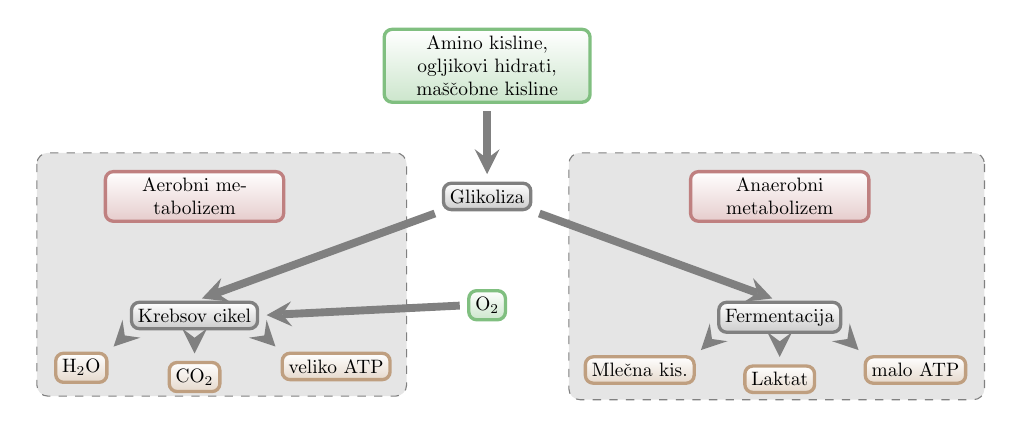
\begin{tikzpicture}
  % LAYERS
  \pgfdeclarelayer{bg}
  \pgfsetlayers{bg,main}
  % LENGTHS
  \newlength{\outdistance}
  \setlength{\outdistance}{4mm}
  %STYLES
  
    
  %
  % Specification of nodes
  %
  \node (food) [input, text width=35mm] {Amino kisline, ogljikovi hidrati, maščobne kisline};
  \node (glycolysis) [block, below = of food] {Glikoliza};
  \node (o2) [input, below = of glycolysis] {O$_2$};
  
  \node (aerobic) [title, left = 2cm of glycolysis] {Aerobni metabolizem};
  \node (krebs) [block, below = of aerobic] {Krebsov cikel};
  \node (aerobic-atp) [output, below right = \outdistance of krebs] {veliko ATP};
  \node (h2o) [output, below left = \outdistance of krebs] {H$_2$O};
  \node (co2) [output, below = \outdistance of krebs] {CO$_2$};
  
  \node (anaerobic) [title, right = 2cm of glycolysis] {Anaerobni metabolizem}; 
  \node (ferment) [block, below = of anaerobic] {Fermentacija};
  \node (anaerobic-atp) [output, below right = \outdistance of ferment] {malo ATP};
  \node (acid) [output, below left = \outdistance of ferment] {Mlečna kis.};
  \node (lactat) [output, below = \outdistance of ferment] {Laktat};
  
  %
  % Specification of lines
  %
  \draw [arrow] (food.south) -- (glycolysis.north);
  \draw [arrow] (glycolysis.south west) -- (krebs.north);
  \draw [arrow] (glycolysis.south east) -- (ferment.north);
  \draw [arrow] (o2.west) -- (krebs.east);
  
  \draw [arrow] (krebs.south west) -- (h2o.north east);
  \draw [arrow] (krebs.south) -- (co2.north);
  \draw [arrow] (krebs.south east) -- (aerobic-atp.north west);
  
  \draw [arrow] (ferment.south west) -- (acid.north east);
  \draw [arrow] (ferment.south) -- (lactat.north);
  \draw [arrow] (ferment.south east) -- (anaerobic-atp.north west);
  
   %
  % Background
  %
  \begin{pgfonlayer}{bg}
  	\node (ltop) [above = 1mm of aerobic] {};
    \node (lleft) [left = 1mm of h2o] {};
  	\node (l0) [] at ( ltop -| lleft) {};
    \node (l1) [below right = 1mm of aerobic-atp] {};
    \path[background] (l0) rectangle (l1);
    
    \node (rtop) [above = 1mm of anaerobic] {};
    \node (rright) [right = 1mm of anaerobic-atp] {};
    \node (r0) [] at (rtop -| rright) {};
    \node (r1) [below left = 1mm of acid] {};
    \path [background] (r0) rectangle (r1);
  \end{pgfonlayer}
\end{tikzpicture}
}
 \caption[Diagram aerobnega in anaerobnega metabolizma]{Diagram aerobnega in anaerobnega metabolizma. Pri aerobnem metabolizmu formacija ATP poteka preko glikolize in Krebsovega cikla, kjer se porablja kisik~\cite{scott2005misconceptions}. Pri anaerobnem metabolizmu se ATP formirajo preko glikolize in fermentacije.}
 \label{fig:metabolism}
\end{figure}

\section{Merjenje energijske porabe}\label{sec:merjenje}
Zaradi kompleksne narave fizične aktivnosti je merjenje energijske porabe velik metodološki izziv~\cite{zhang2004improving}. Zhang et al.~\cite{zhang2004improving} pri tem izpostavlja, da je pomemben del tega problema različen življenjski slog posameznika. 

%Kot smo razložili v poglavju~\ref{sec:energija} je energijska poraba pravzaprav toplota, ki izhaja iz energijskih procesov mišičnih celic~\cite{scott2005misconceptions}. 
Energijsko porabo lahko določimo z merjenjem toplotnih izgub med subjektom in kalorimetrom, saj se teoretično vsa mehanična energija v izoliranem sistemu pretvori v toploto~\cite{levine2005measurement}. Tovrstno merjenje imenujemo \emph{direktna kalorimetrija}~\cite{levine2005measurement}. Merilne naprave za direktno kalorimetrijo so izjemno drage, ki jih uporabljajo le visoko specializirani laboratoriji~\cite{levine2005measurement}. Obstaja več tipov naprav, za vse pa je značilno, da gre za komore, ki zagotavljajo toplotno ravnovesje. Odzivni časi so dokaj dolgi in lahko trajajo do \SI{30}{\min}, merilna napaka pa se giblje med \hbox{\SIrange{1}{2}{\%}}~\cite{levine2005measurement}.

Toplota v človeškem telesu nastaja zaradi aerobnega ali anaerobnega metabolizma~\cite{scott2005misconceptions}. Ker ima anaerobni metabolizem nizko kapaciteto in traja kratek čas~\cite{sahlin1998energy}, se je v športu bolj uveljavilo merjenje aerobne kapacitete~\cite{scott2005misconceptions,howley1995criteria}. Pri aerobnem metabolizmu se za produkcijo toplote porablja kisik, zato lahko energijsko porabo posredno merimo s porabo kisika (${VO}_2$)~\cite{scott2005misconceptions}. Tako merjenje imenujemo \emph{indirektna kalorimetrija}~\cite{levine2005measurement}. Merilne naprave so glede na direktno kalorimetrijo cenejše in manj kompleksne. Večinoma gre za naprave z masko, ki mora biti fiksirana na nos in usta~\cite{levine2005measurement}, zato niso primerne za široko uporabo ali izven-laboratorijske raziskave. Z merilnimi napakami pod \SI{3}{\%} in dokaj hitrimi odzivnimi časi prekašajo metode direktne kalorimetrije~\cite{levine2005measurement}.

Za potrebe terenskih raziskav se je razvila tretja skupina merilnih tehnik, t.i. \emph{nekalorimetrične metode}~\cite{levine2005measurement}. Energijska poraba nastaja zaradi gibanja telesa, zato se nekalorimetrične metode osredotočajo na opazovanje kinematike in ostalih fizioloških parametrov, ki sodelujejo pri fizičnih aktivnostih~\cite{levine2005measurement}. Sem sodijo meritve srčnega utripa, elektromiografija, uporaba pedometrov in pospeškometrov ter brezkontaktne metode.

\subsection{Srčni utrip}\label{sec:srcni-utrip}
Pri zmerni fizični aktivnosti obstaja linearna povezava med srčnim utripom in porabo kisika~\cite{keytel2005prediction}. Kar pa težko rečemo za odnos do energijske porabe, saj obstaja velika varianca med posamezniki~\cite{levine2005measurement}. Ta je odvisna od fizioloških parametrov, kot so spol, višina, teža in telesna pripravljenost. Prav tako na pravilno estimacijo energijske porabe iz srčnega utripa vplivajo emocije in okoljske spremembe~\cite{keytel2005prediction}. Srčni utrip lahko zato uporabimo le v ozkem področju med \SI{90}{bpm} in \SI{150}{bpm}. Vendar tudi tu lahko dobimo razlike na intervalu $[-20~\% , 25~\%]$ glede na meritve indirektnih metod~\cite{keytel2005prediction}. 

Ker je srčni utrip zelo slab posrednik za estimacijo energijske porabe, so raziskovalci predlagali modele, ki upoštevajo dodatne fiziološke parametre~\cite{charlot2014improvement}. Najbolj pogosto citirana modela, ki se uporabljata tudi za široko populacijo, sta \emph{Keytelova modela}~\cite{keytel2005prediction}. Pri prvem modelu~\eqref{eq:keytel1} moramo za izračun energijske porabe $W$ [\si{\kcal\per\min}] poznati spol $s$ ($1$ moški, $0$ ženska), starost $st$ [leto], težo $m$ [\si{\kg}], srčni utrip $hr$ [\si{bpm}] in maksimalno porabo kiska merjenca \vomax [\si{\ml\per\kg\per\min}]. Korelacijski koeficient $CORR$ tega modela glede na indirektno kalorimetrijo znaša \num{0.812}~\cite{charlot2014improvement}.

\begin{align} \label{eq:keytel1}
W = & \num{-59.3954} + s~(\num{-36.3781} + \num{0.271}~st + \num{0.394}~m  \nonumber \\
& + \num{0.404}~v + \num{0.634}~hr ) + (1 - s) \nonumber \\
&\cdot (\num{0.274}~st + \num{0.103}~m + \num{0.380}~VO_{2max} + \num{0.450}~hr)
\end{align}

Drugi Keytelov model~\eqref{eq:keytel2} ne upošteva maksimalne porabe kisika \vomax, ki nam pogosto manjka, in je zato manj točen~\cite{keytel2005prediction}. Njegov korelacijski koeficient \corr znaša \num{0.632}~\cite{charlot2014improvement}.

\begin{align}\label{eq:keytel2}
 W = & s~(\num{-55.0969} + \num{0.6309}~hr + \num{0.1988}~m + \num{0.2017}~st) \nonumber \\
 & + (1 - s) \cdot (\num{-20.4022} + \num{0.4472}~hr - \num{0.1263}~m + \num{0.074}~st)
\end{align}

Charlot et al.~\cite{charlot2014improvement} je z uporabo drugačnih parametrov izboljšala rezultate glede na drugi Keytelov model. Model~\eqref{eq:charlot} je tako dosegel korelacijski koeficient $\corr= \num{0.657}$. Pri tem modelu moramo za izračun energijske porabe $W$ [\si{\kcal\per\hour}]  poznati srčni utrip $hr$ [\si{bpm}], višino $h$ [\si{\cm}], težo $m$ [\si{\kg}], spol $s$ ($1$ moški, $2$ ženski), srčni utrip v mirovanju $hr_r$ [\si{bpm}] in teoretični maksimalni srčni utrip \hrtmax [\si{bpm}]~\cite{charlot2014improvement}. Srčni utrip v mirovanju je definiran kot srednja vrednost srčnega utripa zadnjih dveh minut pet minutnega mirovanja v ležečem položaju. Teoretični maksimalni srčni utrip lahko izračunamo na več različnih načinov. Najbolj pogosto uporabljena enačba za izračun je~\eqref{eq:hrtmax1}, vendar pa obstajajo bolj natačni modeli, kot je enačba~\eqref{eq:hrtmax2}~\cite{miller1993predicting}. 

\begin{align}\label{eq:charlot}
W = & \num{171.62} + \num{6.87}~hr + \num{3.99}~h + \num{2.3}~m \nonumber \\
& - \num{139.89}~s - \num{4.26}~hr_r - \num{4.87}~hr_{tmax}
\end{align}

\begin{align}
	hr_{tmax} = & \num{220} - st \label{eq:hrtmax1}\\ 
    hr_{tmax} = & 217 - \num{0.85}~st \label{eq:hrtmax2}
\end{align}

Slaba lastnost modela~\eqref{eq:charlot} je, da energijsko porabo računamo na urni interval in ne na minutnega, kot je običajno. Pri pretvorbi v minutni interval dobimo približek, saj s tem upoštevamo konstantno vrednost energijske porabe na intervalu $1$ ure. 





\subsection{Senzorji gibanja}\label{sec:senzorji-gibanja}

Za predikcijo energijske porabe iz opazovanja kinematike se večinoma uporabljajo pedometri in pospeškometri~\cite{levine2005measurement}. Pedometri zaznajo premike z vsakim korakom, vendar pa imajo probleme z občutljivostjo. Ker z njimi ne moremo določiti dolžine koraka, so zelo slabi prediktorji in se za tovrstna merjenja ne uporabljajo~\cite{levine2005measurement}.

Merjenje s pospeškometri je lahko dokaj natančno, saj je pospešek sorazmeren zunanjim silam in zato odraža intenziteto gibanja~\cite{yang2010review}. Pri tem moramo paziti, da uporabimo triosne in ne enoosnih pospeškometrov, saj ti ne dajejo zadovoljivih rezultatov~\cite{levine2005measurement}. Pospeškometri se lahko uporabljajo tako za laboratorijske kot tudi za terenske raziskave~\cite{yang2014sleep}, vendar pa, kot pravi Zhang et al~\cite{zhang2004improving}, je njihova natančnost vprašljiva. Faktorji, ki vplivajo na njihovo natančnost, so lokacija, način pritrditve na telo in zunanje vibracije~\cite{yang2010review}. Priporočljivo je, da jih pritrdimo na spodnji del hrbta, saj bomo le tako zajeli večino premikov težišča telesa pri aktivnostih. Za bolj natančne meritve bi morali pospeškometre pritrditi tudi na druge dele telesa, še posebej na okončine~\cite{yang2010review}. To zmanjšuje njihovo praktičnost, saj omejujejo gibanje športnikov in s tem posredno vplivajo na rezultat. Pospeškometri imajo še eno slabo lastnost. Njihova natančnost močno upade, kadar gibanje ni horizontalno s podlago, kar pomeni, da so neuporabni za hojo ali tek v hrib, plezanje, itd.~\cite{yang2010review}.

Za primer študije, ki uporablja kontaktne metode, lahko navedemo~\cite{gjoreski2015context}. V tem delu so avtorji določali energijsko porabo z regresijskimi modeli. Te so učili na večdimenzionalnih vektorjih značilk iz kontaktnih senzorjev.





\subsection{Brezkontaktne metode}

Zaradi omejitev kontaktnih senzorjev, slabih lastnosti srčnega utripa in drage indirektne kalorimetrije, ki se lahko uporablja samo v laboratoriju, so raziskovalci razvili brezkontaktne metode estimacije energijske porabe, kjer dominirajo metode analize video posnetkov~\cite{botton2011energy,osgnach2010energy,silva2015assessing,peker2004framework,nathan2015estimating}. 

\section{Prispevek dela}
Nobena od brezkontaktnih metod estimacije energijske porabe ne izkorišča polja gibanja. To je najbolj optimalna rešitev za sisteme računalniškega vida, ki merijo energijsko porabo, saj je povezana s kinematičnim gibanjem. Polja gibanja ne moremo direktno meriti, zato uporabljamo njegovo aproksimacijo, optični tok. Uporaba optičnega toka je lahko zagotovo bolj natančna od do sedaj predlaganih metod. Seveda tak pristop na podlagi natančnosti ne more nadomestiti indirektne kalorimetrije, lahko pa nadomesti široko uporabljene kontaktne senzorje. Metoda je v primerjavi s kontaknimi senzorji tudi bolj praktična, saj ti omejujejo gibanje in s tem posredno vplivajo na rezultat. 

Pri uporabi optičnega toka lahko veliko elementarnih problemov, kot so problem reže in paralaksa gibanja, rešimo z vpeljavo skrbno izbranih deskriptorjev. Tako lahko metodo uporabimo pri različnih modalitetah. Energijsko porabo lahko merimo iz različnih zornih kotov in z različnimi tipi kamer, kot so: RGB, bližnje-infrardeče (NIR) in globinske kamere (RGB-D). Z uporabo deskriptorjev lahko v postopek pridobivanja energijske porabe učinkovito integriramo regresijske modele s strojnim učenjem, na podlagi podpornih vektrojev in parametrično optimizacijo mrežnega iskanja. 

Vsekakor optični tok ni edini aproksimator polja gibanja. Koncept lahko razširimo na tridimenzionalni prostor z uporabo prostorskega toka. S slednjim lahko močno izboljšamo natančnost postopka, saj dobimo podatke v metričnih enotah. Tudi deskriptorje, ki jih uporabljamo za večjo robustnost optičnega toka, lahko razširimo na več dimenzij in tako obdržimo temeljni del postopka.

Kljub specifični uporabi predlagane metode za merjenje energijske porabe, bi lahko tako metodo uporabili tudi za druge principe gibanja. Koncept merjenja s pomočjo optičnega toka nam omogoča, da opravljamo meritve z daljših razdalj, dokler nam optični sistem zagotavlja stabilno sliko. Tako smo se za prikaz posplošitve našega sistema odločili, da bomo preizkusili naš sistem kot detektor dihanja, saj dihanje, enako kot gibanje, predstavlja vrsto telesne aktivnosti. Detekcija dihanja je podrobneje predstavljena v poglavju~\ref{sec:detekcija-dihanja}

V delu predstavljamo izčrpno študijo o pridobivanju energijske porabe iz podatkov 2D ali 3D slike, brez domnev ali detekcij postavitve skeleta. Preučili smo več modalitet vhodnih podatkov (RGB, NIR in t.i. čas preleta, angl. ``Time-of-flight''), različne pozicije kamer, različne tehnologije za pridobivanje videoposnetkov (IP kamere, vgrajena platforma Raspberry Pi, Microsoft Kinect za Windows V2) in različne kombinacije obdelovalnih elementov (HOOF in HAFA deskriptorji, sledenje, filtriranje, glajenje). Poskusi so bili opravljeni v laboratoriju in na terenu--med tekmami za squash.

V poglavju~\ref{sec:metode}  predstavljamo metode, ki smo jih uporabili v postopku predikcije dihanja in predikcije energijske porabe. V poglavju~\ref{sec:eksperimenti} opisujemo eksperimente in njihove rezultate. Na koncu sledi še diskusija, kjer ovrednotimo rezultate.

Manjši del študije, ki jo predstavljamo v tem delu, je bil objavljen na mednarodni konferenci~\cite{j}
\section{Podobna dela}\label{sec:podobna-dela}



\subsection{Subjektivna primerjava aktivnosti gibanja}\label{sec:subjektivna-primerjava}

Peker et al.~\cite{peker2004framework} zagovarja stališče, da je intenziteta aktivnosti pri opazovanju video posnetkov subjektivna meritev. Pri opazovanju gibanja v video posnetkih bo vsaka oseba zaznala drugačno intenziteto. Vsekakor pa bodo vsi prepoznali hojo kot nizko intenziteto, tek pa visoko intenziteto aktivnosti. Na podlagi tega so zato v delu~\cite{peker2004framework} predstavili izvedbo psihofizičnega protokola za primerjavo meritev intenzitete aktivnosti s pomočjo subjektivne reference.

Subjektivni zlati standard so v~\cite{peker2004framework} določili s 15 merjenci, ki so določevali intenziteto gibanja $294$ video posnetkov dolžine \SI{1.5}{\s} z lestvico od najmanjše do največje intenzitete $0$--$5$. Na podlagi strinjanja o intenziteti gibanja med subjekti, so izračunali mediano in jo uporabili za zlati standard. Glede na standard so avtorji~\cite{peker2004framework} primerjali $9$ različnih deskriptorjev izpeljanih iz vektorjev gibanja. Ugotovili so, da je pravilnost estimacije odvisna od razdalje gibajočih oseb od kamere~\cite{peker2004framework}. Prav tako na pravilnost vpliva tresenje kamere. Na podlagi primerjave srednje napake med deskriptorji so ugotovili, da so MPEG-7 deskriptorji gibanja primerni za uporabo v tovrstni problematiki~\cite{peker2004framework}.

Fiziologija gibanja je v~\cite{peker2004framework} popolnoma izključena. Tu gre zgolj za primerjave med deskriptorji in grobo subjektivno oceno intenzitete aktivnosti, ki ne daje nobenih oprijemljivih informacij. Predstavlja pa dobro usmeritev za uporabo deskriptorjev za namene ocene intenzitete aktivnosti. Ti naj bi temeljili na polju gibanja, ki je tudi najtesneje povezan s fiziologijo. Prav tako opisuje zametke problematike merjenja intenzitete aktivnosti, ko opisuje odvisnost estimacije od razdalje oseb od kamere in njeno premikanje.




\subsection{Predikcija tipov fizične aktivnosti z video analizo}

V študiji~\cite{silva2015assessing} so evaluirali avtomatski sistem za video analizo. S predikcijo tipov fizične aktivnosti so želeli pokazati, da so določene metode računalniškega vida, kot je segmentacija slik, detekcija in sledenje igralcev z uporabo Kalmanovega filtra, ravno tako primerne za določevanje fizične aktivnosti, kot pospeškometri in orodja za ročno označevanje.

Za eksperimente je Silva et al.~\cite{silva2015assessing} uporabil 8 košarkašev, ki so igrali \SI{20}{minutno} igro. Košarkaši so imeli okoli pasu pritrjen pospeškometer Actigraph GT3X+, ki je služil za zlati standard. Za ročno označevanje so uporabili orodje SOPLAY, pri čemer so uporabili dva operaterja (SOPLAY 1 in SOPLAY 2)~\cite{silva2015assessing}. Video sistem (CAM) je bil sestavljen iz ene kamere Gigabit Ethernet camera DFK 31BG03.H, ki je bila pritrjena na strop igrišča. Uporabili so širokokotno lečo Computar T2Z1816CS z goriščnimi razdaljami \SI{1.8}{\mm}--\SI{3.6}{\mm}~\cite{silva2015assessing}. Snemali so z resolucijo $1024$x$768$ in \SI{30}{fps}. S sledenjem igralcev v koordinatnem sistemu igrišča so določili njihove hitrosti~\cite{silva2015assessing}. Na podlagi tega so določili tri tipe fizične aktivnosti in sicer:

\begin{itemize}
\item Lahka fizična aktivnost ($<$\SI{0.9}{m.s^{-1}}),
\item hoja (\SI{0.9}{m.s^{-1}}--\SI{1.8}{m.s^{-1}}) in
\item Fizična aktivnost velike intenzitete ($>$\SI{1.8}{m.s^{-1}})
\end{itemize}

Rezultati dela~\cite{silva2015assessing} so prikazani v tabeli~\ref{tab:silva}. Raziskovalci so ugotovili, da avtomatski sistem za video analizo deluje bolje od ročnega označevanja.

\begin{table}[!htb]
	\centering
    \begin{tabular}{l S[table-format=2.2] S[table-format=1.2]}
    \toprule
    \textbf{Metoda} & \theadm{\chi^2} & \theadm{e~[\si{\%}]} \\
    \midrule
    SOPLAY 1 & 77.60 & 8.68  \\
    SOPLAY 2 & 93.10 & 9.60 \\
    \textbf{CAM} & \boldentry{2}{2}{36.40} & \boldentry{1}{2}{5.32} \\
    \bottomrule
    \end{tabular}
    \caption[Rezultati Silva et al. metod]{Rezultati ročnega anotiranja prvega operaterja (SOPLAY 1), ročnega anotiranja drugega operaterja (SOPLAY 2) in avtomatskega sistema za video analizo (CAM) iz~\cite{silva2015assessing}. Za metriko so uporabili $\chi^2$ in srednjo procentualno napako (e). V tabeli so prikazani samo rezultati primerjave s podatki pospeškometra GT3X. Najboljša metoda je odebeljena.}
    \label{tab:silva}
\end{table}

Za razliko od dela v poglavju~\ref{sec:subjektivna-primerjava} v~\cite{silva2015assessing} že uporabijo objektivne metode, ki ne temeljijo na posameznikovi percepciji intenzivnosti fizične aktivnosti. Avtorji so v delu kategorizirali intenzitete aktivnosti v tri tipe glede na hitrost. V tem pogledu gre le za grobo oceno intenzitete. Ta temelji le na premikanju masnega centra, saj tu ne opazujejo celotnega telesa. Za bolj jasno evaluacijo v~\cite{silva2015assessing} manjkajo uveljavljeni zlati standardi z indirektno metodo. Tu so zlati standard določili s pospeškometri, ki imajo že sami po sebi probleme pri estimaciji kot smo to opisali v~\ref{sec:senzorji-gibanja}.




\subsection{Ocena energijske zahtevnosti igranja nogometa}

V delu~\cite{osgnach2010energy} so avtorji pokazali, da lahko z video analizo in fizikalnim modelom ocenimo energijsko zahtevnost igranja nogometa. Nogomet vsebuje tako aerobne kot anaerobne elemente energijske porabe. Kot navaja Osgnach et al.~\cite{osgnach2010energy} je obremenitev igralcev na tekmo okoli \SI{70}{\%} maksimalne aerobne kapacitete (\vomax). Ti na tekmo porabijo \SI{1200}{\kcal}--\SI{1500}{\kcal}. 

Čeprav so metode, s katerimi so ocenili energijsko porabo in obremenitev v nogometu, zanesljive, ni bilo razvite še nobene, ki bi merila trenutno porabo~\cite{osgnach2010energy}. Takšna metoda bi bila bistveno bolj natančna, saj je energijski profil tega športa bistveno bolj razvejan, kot pa standardne meritve konstantnega teka na tekalni stezi. Igralci so tako \SI{70}{\%} tekme v nizki intenziteti porabe energije (hitra hoja in lahkoten tek), ostalo pa v visoki intenziteti kamor spada sprint~\cite{osgnach2010energy}. 

Osgnach et. al~\cite{osgnach2010energy} zagovarja stališče, da največji del metabolične obremenitve nastane pri pospeševanju in zaviranju, zato so razvili fizikalni model, s katerim lahko določijo energijsko porabo glede na hitrost in pospeške~\cite{osgnach2010energy}. Model predvideva, da sta konstanten tek v hrib in sprint ekvivalentna, saj se telo v času sprinta nagne za določen kot glede na tla.  

Za izračun energijske porabe igralca v \SI{90}{\min} tekmi, so snemali $56$ tekem, kjer je sodelovalo $399$ igralcev~\cite{osgnach2010energy}. Pozicije igralcev v času tekme so določili s polavtomatskim sistemom SICS, ki uporablja štiri \SI{25}{\Hz} kamere. Merilna napaka je bila \SI{1.0}{\%}. Zmogljivost posameznega igralca so določili s tremi parametri, ki so jih razdelili na posamezne kategorije~\cite{osgnach2010energy}:

\begin{itemize}
\item Hitrost ($6$ kategorij),
\item Pospešek ($8$ kategorij) in
\item Metabolična moč ($5$ kategorij).
\end{itemize}

Avtorji so v~\cite{osgnach2010energy} določili, da igralec na tekmo porabi $1107 \pm 119$~kcal, kar se sklada z opažanji ostalih raziskovalcev. Ugotovili so, da je energijska poraba pri različnih hitrostih podobna, saj naj bi bila bolj odvisna od pospeševanja in zaviranja. Ker so tu računali energijsko porabo le iz teka, niso upoštevali drugih aktivnosti kot je skakanje, brcanje žoge, itd. Delo ne zajema nobene primerjave modela z referenčnimi podatki energijske porabe, zato ne moremo z zagotovostjo trditi o njegovi pravilnosti. Sama metoda uporabe fizikalnega modela je omejena na tek, zato ga ne moremo uporabiti za vrsto drugih aktivnosti.





\subsection{Merjenje aktivnosti v tenisu}

Tako kot nogomet, je tudi tenis kompleksen šport, kjer se uporabljata anaerobni in aerobni metabolizem~\cite{botton2011energy}. Obremenite so tu nekoliko manjše, saj dosegajo ravni $<$ \SI{60}{\%}--\SI{70}{\%} \vomax. Tudi v tenisu so estimacije srednje vrednosti energijske porabe neprimerne, saj profil intenzitete fizične aktivnosti ni konstanten. V delu~\cite{botton2011energy} so zato razvili metodo estimacije energijske porabe s pomočjo metaboličnih modelov fundamentalnih aktivnostih. 

Maksimalno aerobno kapaciteto igralcev (\vomax) so določili z inkrementalnim testom na sobnem kolesu Monark 824 z 80 rpm in \SI{20}{W.\min^{-1}} povečevanjem, s čimer so dosegli izčrpanost pod \SI{17}{\min}~\cite{botton2011energy}. Za referenčno določevanje porabe kisika (\vo) med testi pa so uporabili prenosni system za analizo plinov K4B2. 

Profil tenisa  so v~\cite{botton2011energy} razdelili na $5$ fundamentalnih aktivnosti: hoja, tek, sedenje, udarci z loparjem in serviranje. S pomočjo merjenja porabe kisika in linearnim naraščanjem hitrosti hoje in teka ter linearnim naraščanjem frekvence udarcev so določili linearne metabolične modele za posamezno fundamentalno aktivnost. Z njimi so računali metabolično moč. Pri tem so uporabili $8$ teniških igralcev~\cite{botton2011energy}. Metabolične modele so uporabili v poenostavljenih matematičnih ASTRABIO modelih, za opisovanje porabe kisika, aerobne in anaerobne porabe energije, glede na čas izvajanja fundamentalne aktivnosti. 

Čas izvajanja posameznih fundamentalnih aktivnosti so določili s snemanjem in video analizo tekme z Canon MVI 850i digitalno kamero s Canon A28 širokokotno lečo~\cite{botton2011energy}. Kamera je bila postavljena %\SI{6}{m} za igriščem in \SI{5.55}{m} visoko 
tako, da je pokrivala igrišče do mreže. 

Z merjenjem $16$ iger so dobili za estimacijo porabe aerobne energije korelacijski koeficient $\corr = 0.93$~\cite{botton2011energy}. Srednja vrednost porabe kisika je za model znašala \SI{51.7 \pm 10.5}{\%} \vomax. Izmerjena srednja vrednost je bila \SI{52.0 \pm 9.1}{\%} \vomax. Poleg tega so lahko 
v~\cite{botton2011energy} posebej določili aerobno in anaerobno porabo energije. Ugotovili so, da je bilo anaerobne porabe \SI{30}{\%} celotne energije, v času serviranja in udarcev z loparjem pa se je povečala na \SI{95}{\%}.  

Sama metodologija v~\cite{botton2011energy} dokaj natančno določi energijsko porabo za posamezne tipe aktivnosti. Prav tako z različnimi modeli omogoča predikcijo porabe kisika ter anaerobne in aerobne porabe energije. Validacija modelov je trdna, saj so jih avtorji primerjali s standardno indirektno kalorimetrijo. Kljub temu lahko v uporabi metaboličnih modelov opazimo nekaj pomanjkljivosti. Razvoj metaboličnih modelov ni trivialen in zahteva precej časa. Prav tako je omejen na specifično vrsto športa, ki vsebuje fundamentalne aktivnosti. Te pa so s stališča računalniškega vida težje določljive in otežujejo razvoj avtomatskih metod, kjer ne potrebujemo operaterjev.




\subsection{Ocena energijske porabe s Kinect senzorji}

Nathan et al.~\cite{nathan2015estimating} je poskušal oceniti energijsko porabo z Microsoft Xbox Kinect V1. Gre za sistem zajemanja gibanja brez markerjev, kjer se uporablja globinska kamera s strukturirano svetlobo~\cite{nathan2015estimating}. Pridobivanje podatkov s tako napravo je nevsiljivo, zato se merjenec lahko premika svobodno in naravno. 

V~\cite{nathan2015estimating} so napravo uporabili za snemanje skeletnega modela in modeliranja energijske porabe iz mehaničnega dela. Za eksperimente so uporabili $2$ Kinect kameri v razmiku \SI{60}{\stopinj} glede na merjenca. $19$ subjektov je opravljalo $4$ različne vaje najmanj $4$ minute~\cite{nathan2015estimating}. Med vajami so merjenci stoje mirovali, dokler se poraba kisika ni umirila na že prej kalibrirano stojno mirovno metabolično stopnjo. Za zlati standard so uporabili Cortex Metamax 3B avtomatski sistem za analizo plina~\cite{nathan2015estimating}.

Iz premikov posameznih segmentov skeletnega modela so v~\cite{nathan2015estimating} določili različne značilke. Med njimi so določili koncentrične in ekscentrične kontrakcije mišic za masni center, spodnje in zgornje okončine ter faktor drže. Ta je predstavljal količino dela, ki ga porabi telo za ohranitev poze~\cite{nathan2015estimating}. Za predikcijo so uporabili Gaussovo regresijo (GPR), lokalno uteženo regresijo K najbližji sosed (KNNR) in linearno regresijo (LINR). Rezultati modelov v obliki metrik so prikazani v tabeli~\ref{tab:nathan}.

\begin{table}[!htb]
	\centering
    \begin{tabular}{l 
    S[table-format=2.3]
    S[table-format=2.2] 
    S[table-format=1.3]}
    \toprule
    \textbf{Model} & \thead{\rmse [\si{\kJ}]} & \theadm{e~[\si{\%}]} & \thead{CCC} \\
    \midrule
    \textbf{GPR} & \boldentry{2}{3}{8.384} &  35.64 & \boldentry{1}{3}{0.879} \\
    KNNR & 8.415 & 29.76 & 0.847 \\
    LINR & 10.229 & \boldentry{2}{2}{29.39} & 0.847 \\
    \bottomrule
    \end{tabular}
    \caption[Rezultati Nathan et al. modelov]{Rezultati modela Gaussove regresije (GPR), modela lokalno utežene regresije K-najbližji sosed (KNNR) in modela linearne regresije (LINR) iz dela~\cite{nathan2015estimating}. Avtorji so za prikaz rezultatov uporabili koren srednje kvadratne napake (RMSE), srednjo procentualno napako (e) in konkordančni korelacijski koeficient (CCC). Najboljši rezultati posamezne metrike in modela so odebeljeni. Najbolje se je izkazal GPR model~\cite{nathan2015estimating}.}
    \label{tab:nathan}
\end{table}

Avtorji~\cite{nathan2015estimating} so ugotovili, da z njihovo metodo lahko dobro ocenijo energijsko porabo le za aktivnosti visoke intenzitete, kot je skakanje. To omejuje uporabnost take metode, saj  so aktivnosti visoke intenzitete tudi pomembne in lahko bistveno vplivajo na rezultate~\cite{osgnach2010energy}. Prav tako je metoda omejena z opremo, saj moramo imeti senzorje, ki omogočajo razpoznavanje skeleta. Za razliko od prejšnjih del, ki temeljijo na fizičnih in metaboličnih modelih~\cite{osgnach2010energy,botton2011energy}, to metodo lahko apliciramo na različne športe. 


\section{Detekcija dihanja}\label{sec:detekcija-dihanja}
Detekcija dihanja, je zelo pomembna v medicini, saj je dihanje eno izmed osnovnih življenjskih funkcij. Seveda obstaja že veliko literature in aplikacij na to temo~\cite{sathyanarayana2015vision}.

Velik poudarek pri spremljanju dihanja dajejo detekciji  \emph{sindroma spalne apneje}~\cite{sathyanarayana2015vision}. Gre za pogosto in resno zdravstveno stanje~\cite{wang2006vision}, kjer prihaja do krajših zastojev dihanja~\cite{flemons2002obstructive}. Zastoji dihanja se pojavljajo skozi celo noč in zmanjšujejo kvaliteto spanca. Pomanjkanje spanca vpliva na kvaliteto življenja in povečuje nagnjenost k zdravstvenim težavam~\cite{malhotra2002obstructive}. Apneja lahko povzroča depresijo in diabetes. Prav tako je povezana s kardiovaskularnimi obolenji~\cite{takemura2005respiratory}.

Obstajata dva tipa sindroma spalne apneje. Vzrok \emph{centralne spalne apneje} je okvara možganskega centra za nadziranje dihanja~\cite{javaheri2010central}. Možgani so nezmožni generiranja signalov za ritmično dihanje, kar povzroči pomanjkanje respiratornega gibanja prsnega koša in abdomna. \emph{Obstruktivno spalno apnejo} povzroči kolaps mehkega tkiva v grlu. Tkivo zapre dihalne poti, kar povzroči premikanje prsnega koša in abdomna v nasprotni smeri.

Trenutni klinični standard za diagnozo sindroma spalne apneje je \emph{polisomnograf} (PSG)~\cite{collop2007clinical}, kjer uporabljamo različne kontaktne senzorje za meritve različnih fizioloških parametrov~\cite{heinrich2015video}. Ker so senzorji pritrjeni na pacienta, ga zato motijo med spanjem. Kljub problemom kontaktnih senzorjev, so tovrstne meritve dokaj natančne z nizko stopnjo napak. Največji problem polisomnografske meritve je v tem, da je zelo draga in ni primerna za dolgotrajno opazovanje pacientov.

Bolj dostopna alternativa za detekcijo respiratornih motenj je \emph{pulzna oksimetrija}~\cite{netzer2001overnight}. Tu merimo ponavljajoče se fluktuacije v nasičenosti kisika v arterijah ($\mathrm{SpO}_{2}$)~\cite{levy1996accuracy}. Obstaja kar nekaj kazalnikov za predikcijo sindroma spalne apneje, ki so opisani v~\cite{netzer2001overnight, magalang2003prediction}. Najpogosteje se uporablja \SI{4}{\%} zmanjšanje nasičenosti glede na delovno točko signala. Na podlagi raznih raziskav~\cite{cooper1991value,magalang2003prediction,netzer2001overnight,levy1996accuracy} je natančnost oksimetrije podobna natačnosti PSG, zato se lahko uporablja kot alternativa za diagnozo sindroma spalne apneje.

Po drugi strani danes obstaja že kar nekaj brezkontaktnih metod na podlagi računalniškega vida, ki ne motijo spanca in posledično ne ogrožajo rezultatov. Večinoma se uporabljajo infrardeče kamere s sledenjem premikanja prsnega koša~\cite{sathyanarayana2015vision}. Nekateri so poskušali tudi z globinskimi kamerami~\cite{yang2014sleep}, kamerami s časom preleta~\cite{falie2009statistical} in razvojem namenskih senzorjev~\cite{takemura2005respiratory}.

Za sledenje premikanja prsnega koša se uporabljajo standardne metode za detekcijo gibanja. Razliko med slikami so uporabili v delu~\cite{nakai2000non}, optični tok pa v delu~\cite{nakajima2001development}. Ker je dihanje ciklično gibanje in je nagnjeno k okluzijam, avtorji v delu~\cite{wang2014unconstrained} zagovarjajo stališče, da te metode niso primerne za to problematiko. V našem preliminarnem delu~\cite{koporec2017observation} smo pokazali, da lahko z uporabo namenskih deskriptorjev naredimo bolj robusten optični tok, s katerim smo sposobni detektirati dihanje.

%*********************** OSREDNJA POGLAVJA ********************************
\chapter{Metode}\label{sec:metode}


\renewcommand{\folder}{./pogl/02-metode}
\section{Geometrijski model kamere}\label{sec:model-kamere}
Za geometrijski model kamere uporabimo perspektivni model, ki je predstavljen s sliko \ref{fig:perspektivni-model}. Sestavljen je iz slikovne ravnine, koordinatnega sistema kamere in točke prizora \cite{trucco1998introductory}.


\begin{figure}[htb]
\centering
\begin{tikzpicture}%[tdplot_main_coords, scale=0.5]
[x={(0.8cm,0.4cm)}, y={(0cm,1cm)}, z={(0.8cm,-0.4cm)}, scale=0.5]

	% Coordinate system
    \coordinate (O) at (0,0,0);
    \coordinate (oo) at (0,0,5);
    \coordinate (y) at (0,5,0);
    \coordinate (z) at (0,0,15);
    \coordinate (x) at (10,0,0);
    \draw [axis] (O) -- (y) node [right] {$y$};
    \draw [base-axis] (O) -- (oo);
    \draw [axis] (O) -- (x) node [below] {$x$};
    \node (izhodisce) [below] at (O) {$\vec{O}$};
    
    % Image plane
    \coordinate (ol) at (-5,0,5);
    \coordinate (or) at (5,0,5);
    \coordinate (ot) at (0,3,5);
    \coordinate (ob) at (0,-3,5);
    \coordinate (lb) at (-5,-3,5);
    \coordinate (rb) at (5,-3,5);
    \coordinate (lt) at (-5,3,5);
    \coordinate (rt) at (5,3,5);
    \draw [plane] (lb) -- (lt) -- (rt) -- (rb) -- cycle;
    \draw [dash] (ol) -- (or);
    \draw [dash] (ob) -- (ot);
    \node [xshift=3mm, yshift=5mm] at (lb) {$\mathit{\Omega}$};
    % Draw the rest of axis
    \draw [axis] (oo) node [below] {$\vec{c}$} -- (z) node [below] {$z$};
    
    % focal length
    \coordinate (of) at (-5,0,0);
   	\draw [dash] (O) -- (of);
    \draw [<->] (of) -- (ol) node [below] at (-5,0,2.5) {$f$};
    
    % delec
    \coordinate (p) at (5,3,10);
    \draw [fill=black] (p) circle (1.5mm) node [below] {$\vec{p}$};
    \draw [dash, name path=line 1] (O) -- (p);
    \draw [dash] (5,0,0) node [above] {$X$} -- (5,0,10);
    \draw [dash] (0,0,10) node [below] {$Z$} -- (5,0,10);
    \draw [dash] (5,0,10) -- (p);
    
    
    % slika delca
    \coordinate (q) at (2.5,1.5,5);
    \draw [fill=black] (q) circle (1mm) node [below] {$\vec{q}$};
    \draw [dash] (2.5,0,5) node [below] {$x$} -- (q);
    \draw [dash] (0,1.5,5) node [left] {$y$} -- (q);
   
   
\end{tikzpicture}
\caption[Perspektivni model kamere]{Perspektivni model kamere.}
\label{fig:perspektivni-model}
\end{figure}


\textbf{Koordinatni sistem kamere} (KSK) je postavljen tako, da \textbf{optična os} sovpada s $Z$ osjo. Zaradi poenostavitve KSK sovpada z globalnim koordinatnim sistemom.  Središče KSK $\vec{O}$ se imenuje projekcijsko središče, skozi katerega se točka prizora $\vec{p} = \left[ X~Y~Z \right]^\top$ projicira na slikovno ravnino \cite{trucco1998introductory}.

\textbf{Slikovna ravnina} (ang. Image plane) je ravnina $\mathit{\Omega} \subset \mathbb{R}^2$, ki leži na razdalji $f$ od projekcijskega središča $O$. Razdalja $f$ se imenuje goriščna razdalja (ang. Focal length) \cite{trucco1998introductory}. Točka $\vec{c} = \left[c_x~c_y \right]^\top$ se nahaja na poziciji, kjer optična os prebada slikovno ravnino $\mathit{\Omega}$. Imenuje se optično središče slikovne ravnine (ang. Principal point). Točka $\vec{q} = [x~y]^\top$ se nahaja na poziciji, kjer daljica med projekcijskim središčem $\vec{O}$ in točko prizora $\vec{p}$ prebada slikovno ravnino $\mathit{\Omega}$ \cite{trucco1998introductory}. Točka je slika prizora $\vec{q} = [x~y]^\top$, kjer sta $x$ in $y$ slikovni koordinati. Kadar je $\vec{c} = \left[0~0\right]^\top$, lahko sliko $\vec{q}$ na slikovni ravnini $\mathit{\Omega}$ predstavimo z enačbo \eqref{eq:slika-delca}.

\begin{equation}
	\vec{q} = f \frac{\vec{p}}{Z}.
    \label{eq:slika-delca}
\end{equation}

\subsection{Diskretna slikovna ravnina}
Slikovne koordinate so v resnici diskretne, saj sliko sestavlja polje slikovnih elementov $\vec{\lambda}$ s širino $\lambda_u$ in dolžino $\lambda_v$ \cite{trucco1998introductory}. V splošnem je enačba slikovnih koordinat $x$ in $y$ v metričnih enotah \eqref{eq:slikovne-koordinate}, kjer sta $u$ in $v$ slikovni koordinati v pikslih. Točka $\vec{c} = \left[c_u~c_v \right]^\top$ je optično središče v pikslih.

\begin{subequations}
\begin{align}
	x &= \lambda_u (u - c_u) \\
    y &= \lambda_v (v - c_v)
\end{align}
\label{eq:slikovne-koordinate}
\end{subequations}

Če uporabimo homogene koordinate lahko ob upoštevanju enačb \eqref{eq:slika-delca} in \eqref{eq:slikovne-koordinate} izračunamo diskretne slikovne koordinate slike $\vec{q}' = \left[ u~ v \right]^\top$ po enačbi \eqref{eq:diskretne-slikovne-koordinate} \cite{trucco1998introductory}.


\begin{equation}
	w \begin{bmatrix}
	u \\ v \\ 1
	\end{bmatrix} = \vec{M}_{int}
    \begin{bmatrix}
    X \\ Y \\ Z \\ 1
    \end{bmatrix}
    \label{eq:diskretne-slikovne-koordinate}
\end{equation}

Matrika $\vec{M}_{int}$ v enačbi \eqref{eq:diskretne-slikovne-koordinate} je intrinzična matrika \cite{trucco1998introductory}. Predstavljena je z enačbo \eqref{eq:intrinsic} in vsebuje intrinzične parametre kamere, kjer sta $f_u$ in $f_v$ določena z enačbo \eqref{eq:focal}.

\begin{equation}
\vec{M}_{int} = \begin{bmatrix}
	f_u & 0 & c_u & 0 \\
    0 & f_v & c_v & 0 \\
    0 & 0 & 1 & 0
\end{bmatrix}
\label{eq:intrinsic}
\end{equation}

\begin{equation}
\begin{bmatrix}
	f_u & f_v
\end{bmatrix}^\top = \begin{bmatrix}
	\frac{f}{\lambda_u} & \frac{f}{\lambda_v}
\end{bmatrix}^\top
\label{eq:focal}
\end{equation}


\subsection{Premikanje kamere}
Koordinatni sistem kamere lahko transliramo in rotiramo tako, da ne sovpada več z globalnim koordinatnim sistemom, kot je prikazano na sliki \ref{fig:premikanje-kamere}. 

\begin{figure}[htb]
\centering
\begin{tikzpicture}%[tdplot_main_coords, scale=0.5]
[x={(0.8cm,0.4cm)}, y={(0cm,1cm)}, z={(0.8cm,-0.4cm)}, scale=0.5]

	% Coordinate system
    \coordinate (O) at (0,0,0);
    \coordinate (oo) at (0,0,5);
    \coordinate (y) at (0,5,0);
    \coordinate (z) at (0,0,15);
    \coordinate (x) at (10,0,0);
    \draw [axis] (O) -- (y) node [right] {$y$};
    \draw [base-axis] (O) -- (oo);
    \draw [axis] (O) -- (x) node [below] {$x$};
    \node (izhodisce) [below] at (O) {$\vec{O}$};
    
   
    
    
    % Image plane
    \coordinate (ol) at (-5,0,5);
    \coordinate (or) at (5,0,5);
    \coordinate (ot) at (0,3,5);
    \coordinate (ob) at (0,-3,5);
    \coordinate (lb) at (-5,-3,5);
    \coordinate (rb) at (5,-3,5);
    \coordinate (lt) at (-5,3,5);
    \coordinate (rt) at (5,3,5);
    \draw [plane] (lb) -- (lt) -- (rt) -- (rb) -- cycle;
    \draw [dash] (ol) -- (or);
    \draw [dash] (ob) -- (ot);
    \node [xshift=3mm, yshift=5mm] at (lb) {$\mathit{\Omega}$};
    % Draw the rest of axis
    \draw [axis] (oo) node [below] {$\vec{c}$} -- (z) node [below] {$z$};
    
    
    % Coordinate system2
    \begin{scope}{}
    \coordinate (O2) at (1,1,8);
    \coordinate (y2) at (6.7,1.4,6.5);
    \coordinate (z2) at (11.8,-5.4,7.5);
    \coordinate (x2) at (12.4,0.6,-3.1);
    \draw [axis, draw=orange!50!black] (O2) node [below] {$\vec{O}'$} -- (y2) node [above] {$x'$} node (x') [near start] {};
    \draw [axis, draw=orange!50!black] (O2) -- (x2) node [right] {$y'$};
    \draw [axis, draw=orange!50!black] (O2) -- (z2) node [below] {$z'$} node (z') [midway] {};
    \end{scope}
    
    
    
    
    % focal length
    \coordinate (of) at (-5,0,0);
   	\draw [dash] (O) -- (of);
    \draw [<->] (of) -- (ol) node [below] at (-5,0,2.5) {$f$};
    
    % delec
    \coordinate (p) at (5,3,10);
    \draw [fill=black] (p) circle (1.5mm) node [below] {$\vec{p}$};
    \draw [dash, name path=line 1] (O) -- (p);
    \draw [dash] (x') node [above] {$X'$} -- (5,0,10);
    \draw [dash] (z') node [below] {$Z'$} -- (5,0,10);
    \draw [dash] (5,0,10) -- (p);
    
    
    % slika delca
    \coordinate (q) at (2.5,1.5,5);
    \draw [fill=black] (q) circle (1mm) node [below] {$\vec{q}$};
    \draw [dash] (2.5,0,5) node [below] {$x$} -- (q);
    \draw [dash] (0,1.5,5) node [left] {$y$} -- (q);
   
   
\end{tikzpicture}
\caption[Koordinatni sistem kamere in globalni koordinatni sistem]{Koordinatni sistem kamere (KSK) in globalni koordinatni sistem (GKS). KSK je predstavljen s črnimi osmi. GKS je predstavljen z rdečimi osmi. Koordinatna sistema med sabo ne sovpadata.}
\label{fig:premikanje-kamere}
\end{figure}

Translacijo koordinatnega sistema kamere lahko opišemo z vektorjem $\vec{t} = \left[t_x~t_y~t_z\right]^\top$ \cite{trucco1998introductory}. 

Rotacijo koordinatnega sistema kamere lahko opišemo z Eulerjevimi koti $\phi$ $\theta$ in $\psi$ \cite{bajd2011osnove}. S kotom $\phi$ rotiramo okoli $z$ osi (ang. Roll). Rotacija je predstavljena z enačbo \eqref{eq:roll}. Kot $\theta$ predstavlja rotacijo okoli $x$ osi (ang. Pitch). Rotacija je opisana z enačbo \eqref{eq:pitch}. Kot $\psi$ je rotacija okoli $y$ osi (ang. Yaw) in je opisana z enačbo \eqref{eq:yaw}.

\begin{equation}
\vec{R}_\phi = \begin{bmatrix}
\cos(\phi) & - \sin(\phi) & 0 \\
\sin(\phi) & \cos(\phi) & 0 \\
0 & 0 & 1
\end{bmatrix}
\label{eq:roll}
\end{equation}

\begin{equation}
\vec{R}_\theta = \begin{bmatrix}
1 & 0 & 0 \\
0 & \cos(\theta) & - \sin(\theta) \\
0 & \sin(\theta) & \cos(\theta)
\end{bmatrix}
\label{eq:pitch}
\end{equation}

\begin{equation}
\vec{R}_\psi = \begin{bmatrix}
\cos(\psi) & 0 & \sin(\psi) \\
0 & 1 & 0 \\
- \sin(\psi) & 0 & \cos(\psi) 
\end{bmatrix}
\label{eq:yaw}
\end{equation}


Kadar opravimo vse rotacije osi glede na fiksni globalni koordinatni sistem po vrstnem redu $\vec{R}_\psi$, $\vec{R}_\theta$ in $\vec{R}_\phi$, lahko rotacijsko matriko $\vec{R}$ opišemo z enačbo \eqref{eq:rotation} \cite{bajd2011osnove}.


\begin{equation}
\vec{R} = \vec{R}_\phi \vec{R}_\theta \vec{R}_\psi
\label{eq:rotation}
\end{equation}


Translacijo $\vec{t}$ in rotacijo $\vec{R}$ lahko združimo v matriko premika koordinatnega sistema kamere glede na globalni koordinatni sistem, ki jo imenujemo \textbf{ekstrinsična matrika} \cite{trucco1998introductory}. Opisana je z enačbo \eqref{eq:extrinsic}.

\begin{equation}
\vec{M}_{ext} = \begin{bmatrix}
	\vec{R} & \vdots & \vec{t}
\end{bmatrix}
\label{eq:extrinsic}
\end{equation}


Z upoštevanjem premika kamere lahko enačbo \eqref{eq:diskretne-slikovne-koordinate} zapišemo v obliko \eqref{eq:diskretne-slikovne-koordinate-premik}. Matrika $\vec{M}$ je \textbf{projekcijska matrika} in je opisana v enačbi \eqref{eq:projection-matrix}.

\begin{equation}
w \begin{bmatrix}
	u \\ v \\ 1
	\end{bmatrix} = \vec{M}
    \begin{bmatrix}
    X \\ Y \\ Z \\ 1
    \end{bmatrix}
\label{eq:diskretne-slikovne-koordinate-premik}
\end{equation}


\begin{equation}
\vec{M} = \vec{M}_{int} \vec{M}_{ext}
\label{eq:projection-matrix}
\end{equation}

\section{Model gibanja}\label{sec:model-gibanja}
% Ponovi teorijo energijske porabe in kako pridemo do gibanja
% Dokazi, da lahko gibanje opazujemo s kamerami
% Teorija, da je najboljši približek optični tok
Da mišice lahko s svojimi kontrakcijami spravijo telo v pogon, potrebujejo energijo, pri tem pa se del energije pretvarja v toploto, ki ji pravimo energijska poraba \cite{scott2005misconceptions}. Energijska poraba nastaja zaradi gibanja telesa, zato jo lahko določimo z opazovanjem kinematike \cite{levine2005measurement}. Zaradi omejitev kontaktnih senzorjev in slabih lastnosti srčnega utripa so v študijah, ki so opisane v poglavju \ref{sec:podobna-dela}, dokazali, da lahko z opazovanjem kinematike z računalniškim vidom določimo energijsko porabo. 

Predpostavimo perspektivni model kamere, ki je opisan v poglavju \ref{sec:model-kamere}.
Naj bo delec z maso $m$ predstavljen kot točka prizora $\vec{p}$, na sliki \ref{fig:model-gibanja}. Gibanje delca $\vec{p}$ lahko predstavimo z vektorjem hitrosti $\vec{v} = [v_X~v_Y~v_Z]^\top$, $\vec{v} \in \mathcal{V} \subset \mathbb{R}^3$, kjer so $v_X$, $v_Y$ in $v_Z$ hitrosti glede na osi in $\mathcal{V}$ vektorski prostor. Kadar imamo v prostoru več masnih delcev, množico vektorjev hitrosti imenujemo \textbf{polje hitrosti} (angl. Velocity Field) $\mathbf{H}: \mathbb{R}^3 \to \mathcal{V}$, kjer velja $\vec{p} \mapsto \vec{v}$ \cite{trucco1998introductory}.


\begin{figure}[htb]
\centering
\begin{tikzpicture}%[tdplot_main_coords, scale=0.5]
[x={(0.8cm,0.4cm)}, y={(0cm,1cm)}, z={(0.8cm,-0.4cm)}, scale=0.5]
      
	% Coordinate system
    \coordinate (O) at (0,0,0);
    \coordinate (y) at (0,5,0);
    \coordinate (z) at (0,0,15);
    \coordinate (x) at (10,0,0);
    \draw [axis] (O) -- (y) node [above] {$y$};
    \draw [axis] (O) -- (z) node [below] {$z$};
    \draw [axis] (O) -- (x) node [below] {$x$};
    \node (izhodisce) [below] at (O) {$o$};
    
    % delec
    \coordinate (p) at (5,3,10);
    \draw [fill=black] (p) circle (1.5mm) node [below] {$\vec{p}$};
    \draw [dash] (O) -- (p);
    \draw [dash] (5,0,0) node [above] {$X$} -- (5,0,10);
    \draw [dash] (0,0,10) node [below] {$Z$} -- (5,0,10);
    \draw [dash] (5,0,10) -- (5,3,10);
    
    % hitrost
    \draw [velocity] (p) -- (6,4,10) node [above] {$\vec{v}$};
    

\end{tikzpicture}
\caption[Predstavitev delca $\vec{p}$ v koordinatnem sistemu kamere]{Predstavitev delca $\vec{p}$ v koordinatnem sistemu kamere. Delec je predstavljen kot točka prizora z vektorjem hitrosti $\vec{v}$ \cite{trucco1998introductory}.}
\label{fig:model-gibanja}
\end{figure}



Relativno gibanje delca $\vec{p}$ glede na koordinatno izhodišče kamere $\vec{O}$ lahko opišemo kot:

\begin{equation}
	\vec{v} = -\vec{T}-\omega\times\vec{p},
\end{equation}

kjer je $\vec{T}$ translatorna hitrost in $\omega$ kotna hitrost \cite{trucco1998introductory}. Po komponentah lahko gibanje opišemo z enačbo \eqref{eq:gibanje}

\begin{equation} \label{eq:gibanje}
	\begin{bmatrix}
	v_X \\ v_Y \\ v_Z
	\end{bmatrix}
    =
    \begin{bmatrix}
    - T_X - \omega_Y Z + \omega_Z Y \\
    - T_Y - \omega_Z X + \omega_X Z \\
    - T_Z - \omega_X Y + \omega_Y X
    \end{bmatrix}.
\end{equation}

Gibanje telesa v prostoru torej lahko opišemo s poljem hitrosti $\vec{H}$.



\section{Optični tok} \label{sec:opticni-tok}
% Teorija optičnega toka
% vrste optičnega toka
% Kateri tip smo mi uporabili
% Zakaj smo tega uporabili
% Kako smo ga uporabili
% Problemi naše predpostavke
% Rešitev s kalibracijo velikosti
Za namen razlage upoštevamo perspektivni model kamere iz poglavja~\ref{sec:model-kamere} in model gibanja iz poglavja~\ref{sec:model-gibanja}. Dodatno upoštevamo da se osvetlitev ne spreminja.

$\vec{q}$ je slika delca $\vec{p}$ na slikovni ravnini $\varOmega$ Delec in njegova slika sta predstavljena na sliki~\ref{fig:optical-flow} S časovnim odvodom enačbe~\eqref{eq:slika-delca}, dobimo hitrost delca na slikovni ravnini:

\begin{equation}\label{eq:hitrost-slike-delca}
	\vec{u} = f \frac{Z\vec{v}-v_Z\vec{p}}{Z^2},
\end{equation}

kjer je $\vec{u} \in \mathcal{U} \subset \mathbb{R}^2$.




\begin{figure}[htb]
\centering
\begin{tikzpicture}%[tdplot_main_coords, scale=0.5]
[x={(0.8cm,0.4cm)}, y={(0cm,1cm)}, z={(0.8cm,-0.4cm)}, scale=0.5]

	% Coordinate system
    \coordinate (O) at (0,0,0);
    \coordinate (oo) at (0,0,5);
    \coordinate (y) at (0,5,0);
    \coordinate (z) at (0,0,15);
    \coordinate (x) at (10,0,0);
    \draw [axis] (O) -- (y) node [above] {$y$};
    \draw [base-axis] (O) -- (oo);
    \draw [axis] (O) -- (x) node [below] {$x$};
    \node (izhodisce) [below] at (O) {$o$};
    
    % Image plane
    \coordinate (ol) at (-5,0,5);
    \coordinate (or) at (5,0,5);
    \coordinate (ot) at (0,3,5);
    \coordinate (ob) at (0,-3,5);
    \coordinate (lb) at (-5,-3,5);
    \coordinate (rb) at (5,-3,5);
    \coordinate (lt) at (-5,3,5);
    \coordinate (rt) at (5,3,5);
    \draw [plane] (lb) -- (lt) -- (rt) -- (rb) -- cycle;
    \draw [dash] (ol) -- (or);
    \draw [dash] (ob) -- (ot);
    \node [xshift=3mm, yshift=5mm] at (lb) {$\mathit{\Omega}$};
    % Draw the rest of axis
    \draw [axis] (oo) -- (z) node [below] {$z$};
    
    % focal length
    \coordinate (of) at (-5,0,0);
   	\draw [dash] (O) -- (of);
    \draw [<->] (of) -- (ol) node [below] at (-5,0,2.5) {$f$};
    
    % delec
    \coordinate (p) at (5,3,10);
    \draw [fill=black] (p) circle (1.5mm) node [below] {$\vec{p}$};
    \draw [dash, name path=line 1] (O) -- (p);
    \draw [dash] (5,0,0) node [above] {$X$} -- (5,0,10);
    \draw [dash] (0,0,10) node [below] {$Z$} -- (5,0,10);
    \draw [dash] (5,0,10) -- (p);
    
    % hitrost
    \coordinate (v) at (6,4,10);
    \draw [velocity] (p) -- (v) node [above] {$\vec{v}$};
    \draw [dash] (O) -- (v);
    
    % slika delca
    \coordinate (q) at (2.5,1.5,5);
    \draw [fill=black] (q) circle (1mm) node [below] {$\vec{q}$};
    \draw [dash] (2.5,0,5) node [below] {$x$} -- (q);
    \draw [dash] (0,1.5,5) node [left] {$y$} -- (q);
    
    %hitrost
    \draw [velocity] (q) -- (3,2,5) node [above] {$\vec{u}$};

\end{tikzpicture}
\caption[Preslikava hitrosti delca na slikovno ravnino $\varOmega$]{Pri preslikavi polja hitrosti $\vec{H}$ na slikovno ravnino $\varOmega$ dobimo optični tok $\vec{O}$. V koordinatnem sistemu kamere (KSK) ima gibajoči delec $\vec{p}$ s hitrostjo $\vec{v} \in \vec{H}$ sliko $\vec{q}$ s hitrostjo polja gibanja $\vec{u} \in \vec{G}$. V resnici lahko dobimo le aproksimacijo vektorja polja gibanja $\vec{u}$. Aproksimacija je vektor optičnega toka $\vec{w} \in \vec{O}$.}
\label{fig:optical-flow}
\end{figure}




Razširjena oblika enačbe~\eqref{eq:hitrost-slike-delca}, kjer upoštevamo~\eqref{eq:gibanje}, je zapisana z enačbo~\eqref{eq:hitrost-slike-delca-raz}~\cite{trucco1998introductory}. Prvi člen v posamezni enačbi predstavlja \emph{translatorni del}, ostali členi pa sodijo v \emph{rotacijski del}.

\begin{equation}\label{eq:hitrost-slike-delca-raz}
\begin{aligned}
	u_x = & \frac{T_Z x - T_X f}{Z} - \omega_Y f + \omega_Z y + \frac{\omega_X x y}{f} - \frac{\omega_Y x^2}{f} \\
    u_y = & \frac{T_Z y - T_Y f}{Z} - \omega_X f + \omega_Z x + \frac{\omega_Y x y}{f} - \frac{\omega_X y^2}{f}
\end{aligned}
\end{equation}

Kadar imamo na slikovni ravnini več slik delcev, množico vektorjev hitrosti $\vec{u}$ imenujemo \emph{polje gibanja} (angl. Motion Field) $\vec{G} : \varOmega \to \mathcal{U}$, kjer velja $ \vec{q} \mapsto \vec{u}$~\cite{trucco1998introductory}. Polje gibanja $\vec{G}$ lahko razumemo kot projekcijo polja hitrosti $\vec{H}$ na slikovno ravnino, zato ta predstavlja idealno rekonstrukcijo gibanja. V praksi do polja gibanja ne moremo dostopati, zato se poslužujemo njegovih približkov.  

Video posnetek je sestavljen iz sekvence slik, to pa lahko opišemo kot funkcijo osvetljenosti slikovnega elementa $I(\vec{x},t)$, na poziciji $\vec{x} = [x~y]^\top$ ob času $t$~\cite{wedel2011stereo}. Gibanje oseb opazimo kot premikanje pikslov skozi čas, pri čemer predpostavimo, da osvetljenost posameznega piksla ostaja konstantna~\cite{trucco1998introductory}. Stacionarnost osvetljenosti slikovnega elementa lahko opišemo z enačbo  

\begin{equation}
	\frac{d I(\vec{x}, t)}{dt} = \frac{\partial I}{\partial x} \frac{dx}{dt} + \frac{\partial I}{\partial y} \frac{dy}{dt} + \frac{\partial I}{\partial t} = 0,
\end{equation}

to pa lahko zapišemo z vektorjem hitrosti slikovnega elementa $\vec{w} \in \mathcal{W} \subset \mathbb{R}^2$ v kompaktnejšo obliko

\begin{equation}\label{eq:opticni-tok}
	(\nabla I)^\top \vec{w} + I_t = 0.
\end{equation}

Enačba~\eqref{eq:opticni-tok} predstavlja \emph{omejitev optičnega toka}~\cite{trucco1998introductory}. Če v enačbi~\eqref{eq:opticni-tok} normaliziramo prostorski gradient $(\nabla I)$, v enačbi~\eqref{eq:aperture-problem} opazimo, da lahko  določimo le hitrost, ki je vzporedna prostorskemu gradientu. Pojav je znan kot problem reže (angl. Aperture problem)~\cite{trucco1998introductory}. 

\begin{equation}\label{eq:aperture-problem}
	\frac{(\nabla I)^\top \vec{w}}{\| \nabla I \|} = - \frac{I_t}{\| \nabla I \|} = \vec{w}_n
\end{equation}

\emph{Problem reže} si lahko razlagamo na način opazovanja gibanja daljice na beli podlagi skozi režo tako, da ne vidimo koncev. Zaradi omejene vizualne informacije lahko določimo hitrost le v pravokotni smeri na daljico~\cite{trucco1998introductory}. Razlaga je predstavljena na sliki~\ref{fig:aperture-problem}.




\begin{figure}[htb]
\centering
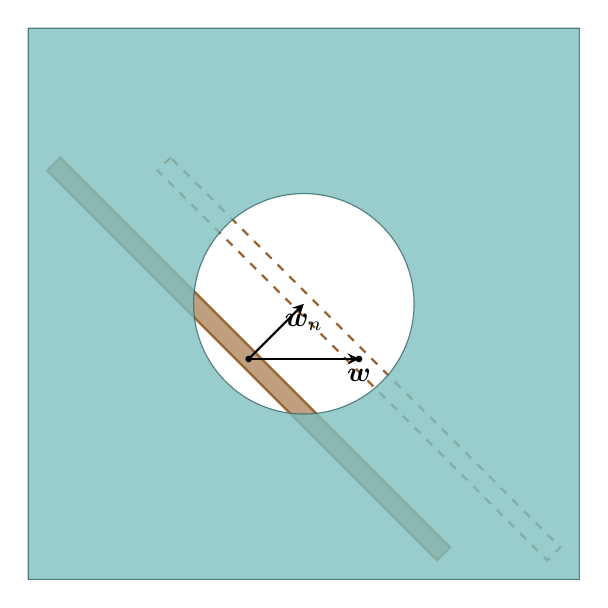
\begin{tikzpicture}[scale=0.7]
\tikzset{aperture/.style = {
fill=teal!50, 
draw=teal!50!black!80
}}
\tikzset{stick/.style = {
fill=orange!50!black!50, 
draw=orange!50!black!80, solid, thick,
minimum width = 1mm, minimum height=7cm
}}
  \begin{scope}
  		\coordinate (top) at (10,10);
        \coordinate (bottom) at (0,0);
       	\coordinate (center) at (5,5);

  		% palica
        \coordinate (pc) at (4,4);
        \path (pc) node[stick,rotate = 45]{};
        \draw [fill] (pc) circle (0.5mm);
        \coordinate (pc2) at (6,4);
        \path (pc2) node[stick, rotate = 45, dashed, fill=none]{};
        \draw [fill] (pc2) circle (0.5mm);
        
        % vektor
        \draw [velocity, draw=black] (pc) -- ++(1,1) node [below] {${\vec{w}_n}$};
        \draw [velocity, draw=black] (pc) -- (pc2) node [below] {$\vec{w}$};
  		% aperture	
		\draw [aperture, opacity=0.8] (bottom) rectangle (top) (center) circle (20mm);  
  \end{scope}


\end{tikzpicture}
\caption[Problem reže]{Problem reže. Ker skozi režo ne vidim koncev daljice, lahko določimo le hitrost v pravokotni smeri na daljico $\vec{w}_n$~\cite{trucco1998introductory}.}
\label{fig:aperture-problem}
\end{figure}




Kadar imamo na slikovni ravnini več premikajočih slikovnih elementov, vektorsko polje hitrosti $\vec{w}$ imenujemo \emph{optični tok} (angl. Optical flow) $\vec{O}: \varOmega \to \mathcal{W}$, kjer velja $ \vec{q} \mapsto \vec{w}$~\cite{trucco1998introductory}. Optični tok je dobra aproksimacija polja gibanja v točkah visokega prostorskega gradienta svetlosti in konstantne osvetlitve.



\subsection{Metode estimacije optičnega toka}\label{sec:metode-of}

Metode estimacije optičnega toka $\vec{O}$ v grobem delimo na diferencialne in {ujemalne} metode~\cite{trucco1998introductory}. Z \emph{diferencialnimi metodami} računamo optični tok z uporabo parcialnih diferencialnih enačb ali minimizacijskimi metodami. Z metodami dobimo \emph{gost optični tok}, kar pomeni, da je optični tok določen za vsak slikovni element~\cite{trucco1998introductory}. Te metode zelo natačno opisujejo optični tok in ne proizvajajo vrednosti, ki lokalno odstopajo, zato je optični tok gladek~\cite{brox2011large}.  Glavni problem teh metod je, da so računsko zelo zahtevne~\cite{trucco1998introductory}.

Pri \emph{ujemalnih metodah} računamo optični tok le na značilnih točkah~\cite{trucco1998introductory}. Zaradi uporabe značilk so te metode lahko bolj efektivne, saj ne potrebujemo določevanja korespondenc za vse piksle. Prav tako se lahko uporabijo za računanje optičnega toka v realnem času, saj niso računsko zahtevne. Po~\cite{trucco1998introductory} je največja težava teh metod, da računajo \emph{redek optični tok}, saj je ta določen le za slikovne elemente, ki predstavljajo značilne točke. Prav tako delujejo dobro le pri majhnih premikih, ker temeljijo na Taylorjevi aproksimaciji enačbe~\eqref{eq:opticni-tok}~\cite{wedel2011stereo}. 

V nadaljevanju predstavljamo diferencialno metodo Farneb{\"a}ck algoritem.

\subsubsection{Farneb{\"a}ck algoritem.}
Algoritem temelji na estimaciji premika z razčlenjevanjem polinoma  po enačbi~\eqref{eq:polinom}, kjer je $\vec{A}$ simetrična matrika, $\vec{b}$ vektor in $c$ skalar~\cite{farneback2003two}.

\begin{equation}\label{eq:polinom}
	f(\vec{x}) \sim \vec{x}^\top \vec{A} \vec{x} + \vec{b}^\top \vec{x} + c
\end{equation}

Ideja temelji na tem, da aproksimiramo okolico piksla s kvadratičnim polinomom, pri čemer želimo najti premik piksla na poziciji $\vec{x}$ z minimizacijo enačbe~\eqref{eq:polinom-min} in omejitvijo~\eqref{eq:omejitev-polinoma}. $\vec{A}_1(\vec{x})$ in $\vec{b}_1(\vec{x})$ sta razčlenitvena koeficienta za prvo sliko, $\vec{A}_2(\vec{x})$ in $\vec{b}_2(\vec{x})$ koeficienta za drugo sliko in $w(\Delta\vec{x})$ je utežna funkcija za sosedne točke.

\begin{align}
\vec{A}(\vec{x}) = & \frac{\vec{A}_1(\vec{x} + \vec{A}_2(\vec{x}))}{2} \\
\Delta\vec{b}(\vec{x}) = & - \frac{1}{2}\left(\vec{b}_2(\vec{x}) - \vec{b}_1(\vec{x})\right) 
\end{align}

\begin{equation}\label{eq:polinom-min}
\sum_{\Delta x \in I} w(\Delta\vec{x}) \| \vec{A}(\vec{x} + \Delta\vec{x})\vec{d}(\vec{x}) - \Delta\vec{b}(\vec{x} +\Delta\vec{x}) \|^2
\end{equation}

\begin{equation}\label{eq:omejitev-polinoma}
\vec{A}(\vec{x})\vec{d}(\vec{x}) = \Delta\vec{b}(\vec{x})
\end{equation}

Rešitev minimizacije enačbe~\eqref{eq:polinom-min} je enačba~\eqref{eq:polinom-resitev}

\begin{equation}\label{eq:polinom-resitev}
 \vec{d}(\vec{x}) = \left( \sum w \vec{A}^\top \vec{a} \right)^{-1} \sum w \vec{A}^\top \Delta\vec{b}
\end{equation}

Evaluacija algoritma je bila narejena v~\cite{Geiger2012CVPR}. Rezultati so povzeti v tabeli~\ref{tab:farneback}. Algoritem so preverjali s procesorjem z 1 jedrom \@ \SI{2.5}{GHz}.

\begin{table}[htb]
	\centering
    \begin{tabular}{S[table-format=2.2] S[table-format=2.2] S[table-format=2.1] S[table-format=2.1] S[table-format=3.2] S[table-format=1]}
    \toprule
    \multicolumn{1}{c}{\emph{Out-Noc}} & \multicolumn{1}{c}{\emph{Out-All}} & \multicolumn{1}{c}{\emph{Avg-Noc}} & \multicolumn{1}{c}{\emph{Avg-All}} & \multicolumn{1}{c}{\emph{Gostota}} & \multicolumn{1}{c}{\emph{Čas izvajanja}} \\
    \midrule
    47.59~\% & 54.00~\% & 17.3~px & 25.3~px & 100.00~\% & 1~s\\
    \bottomrule
    \end{tabular}
    \caption[Evaluacija Farneb{\"a}ck algoritma v KITTI Vision Benchmark 2012]{Evaluacija Farneb{\"a}ck algoritma v KITTI Vision Benchmark 2012~\cite{Geiger2012CVPR}. Metrika Out-Noc predstavlja procent pikslov, ki težijo k napakam v območju, kjer ni prekrivnosti. Out-all je procent pikslov, ki težijo k napakam v celoti. Avg-Noc je povprečna napaka disparitete v območjih neprekrivnosti. Avg-All je povprečna napaka disparitete v celoti. Gostota predstavlja procent pikslov, za katere je metoda določila referenco~\cite{Geiger2012CVPR}.}
    \label{tab:farneback}
\end{table}

\section{Prostorski tok}
% Teorija prostorskega toka
% Katero metodo smo mi uporabili in zakaj
Optični tok $\vec{O}$ predstavlja aproksimacijo polja gibanja $\vec{G}$, ta pa je projekcija polja hitrosti $\vec{H}$ na slikovno ravnino $\mathit{\Omega}$ \cite{trucco1998introductory}. Če pogledamo z druge perspektive, ni optični tok $\vec{O}$ nič drugega kot projekcija aproksimacije polja hitrosti $\vec{H}$, ki jo po analogiji lahko imenujemo \textbf{prostorski tok} (angl. Scene Flow) \cite{vedula1999three}. 

Za namen razlage upoštevamo enake omejitve kamere, masnega delca in osvetlitve, kot v poglavju \ref{sec:opticni-tok}. Predpostavimo, da imamo v prostoru površino $f(x,y,z) = 0$ na kateri imamo gibajoč točkovni delec $\vec{p} = \vec{p}(t)$. Na slikovni ravnini $\mathit{\Omega}$ imamo njegovo sliko $\vec{q}$ \cite{vedula1999three}. Vizualni prikaz prizora lahko vidimo na sliki \ref{fig:scene-flow}. 




\begin{figure}[htb]
\centering
\begin{tikzpicture}%[tdplot_main_coords, scale=0.5]
[x={(0.8cm,0.4cm)}, y={(0cm,1cm)}, z={(0.8cm,-0.4cm)}, scale=0.5]

	% Coordinate system
    \coordinate (O) at (0,0,0);
    \coordinate (oo) at (0,0,5);
    \coordinate (y) at (0,5,0);
    \coordinate (z) at (0,0,15);
    \coordinate (x) at (10,0,0);
    \draw [axis] (O) -- (y) node [above] {$y$};
    \draw [base-axis] (O) -- (oo);
    \draw [axis] (O) -- (x) node [below] {$x$};
    \node (izhodisce) [below] at (O) {$o$};
    
    % Image plane
    \coordinate (ol) at (-5,0,5);
    \coordinate (or) at (5,0,5);
    \coordinate (ot) at (0,3,5);
    \coordinate (ob) at (0,-3,5);
    \coordinate (lb) at (-5,-3,5);
    \coordinate (rb) at (5,-3,5);
    \coordinate (lt) at (-5,3,5);
    \coordinate (rt) at (5,3,5);
    \draw [plane] (lb) -- (lt) -- (rt) -- (rb) -- cycle;
    \draw [dash] (ol) -- (or);
    \draw [dash] (ob) -- (ot);
    \node [xshift=3mm, yshift=5mm] at (lb) {$\mathit{\Omega}$};
    % Draw the rest of axis
    \draw [axis] (oo) -- (z) node [below] {$z$};
    
    % focal length
    \coordinate (of) at (-5,0,0);
   	\draw [dash] (O) -- (of);
    \draw [<->] (of) -- (ol) node [below] at (-5,0,2.5) {$f$};
    
    % povrsina
    \begin{scope}
    \coordinate (p0) at (3,1,12);
    \coordinate (p1) at (3,5,12);
    \coordinate (p2) at (7,5,12);
    \coordinate (p3) at (7,1,12);
   
    \draw [plane, fill=purple!20, draw=purple!50!black!50,] 
    			   (p0) .. controls (3,4,10) .. (p2)
                        .. controls (7,3,10) .. (p3) 
                        .. controls (5,1,10) .. cycle;
    \node at (6,2,12) {$f$};
    \end{scope}
    
    
    
    % delec
    \coordinate (p) at (5,3,10);
    \draw [fill=black] (p) circle (1.5mm) node [below] {$\vec{p}$};
    \draw [dash, name path=line 1] (O) -- (p);
    %\draw [dash] (5,0,0) node [above] {$X$} -- (5,0,10);
    %\draw [dash] (0,0,10) node [below] {$Z$} -- (5,0,10);
    %\draw [dash] (5,0,10) -- (p);
    
    % hitrost
    \coordinate (v) at (6,4,10);
    \draw [velocity] (p) -- (v) node [above] {$\vec{\mu}$};
    \draw [dash] (O) -- (v);
    
    % slika delca
    \coordinate (q) at (2.5,1.5,5);
    \draw [fill=black] (q) circle (1mm) node [below] {$\vec{q}$};
    \draw [dash] (2.5,0,5) node [below] {$x$} -- (q);
    \draw [dash] (0,1.5,5) node [left] {$y$} -- (q);
    
    %hitrost
    \draw [velocity] (q) -- (3,2,5) node [above] {$\vec{w}$};
\end{tikzpicture}
\caption[Vizualni prikaz vektorja prostorskega toka $\vec{w}$]{Vizualni prikaz vektorja prostorskega toka $\vec{w}$. V prostoru imamo površino $f$ na kateri leži gibajoči točkovni delec $\vec{p}$ \cite{vedula1999three}. Na slikovni ravnini $\mathit{\Omega}$ imamo sliko delca $\vec{q}$ s prostorskim tokom $\vec{w}$.}
\label{fig:scene-flow}
\end{figure}



Ker je slika projekcija delca na slikovno ravnino $\mathit{\Omega}$, lahko zapišemo $\vec{q} = \vec{q}(\vec{p})$. Hitrost slike določimo po enačbi \eqref{eq:opticni-tok-sf}, ki predstavlja enačbo vektorja optičnega toka $\vec{w}$, kot projekcijo prostorskega toka \cite{vedula1999three}. 


\begin{equation}\label{eq:opticni-tok-sf}
	\vec{w} = \frac{d\vec{q}}{dt} = \frac{\partial \vec{q}}{\partial \vec{p}}\frac{d\vec{p}}{dt}
\end{equation}

Če predpostavimo, da imamo dovoj informacije o sistemu, da lahko določimo inverzno funkcijo $\vec{p} = \vec{p}(\vec{q},t)$, kjer je masni delec $\vec{p}$ projekcija slike $\vec{q}$, lahko določimo njegovo hitrost $\vec{\mu} \in \mathcal{\Mu} \subset \mathbb{R}^3$ z enačbo \eqref{eq:scene-flow}. Slednja je sestavljena iz dveh delov. Prvi člen je projekcija vektorja optičnega toka $\vec{w}$ na tangentno ravnino površine $f$, v točki, kjer se nahaja delec $\vec{p}$ \cite{vedula1999three}. Drugi člen je hitrost spreminjanja oddaljenosti delca od slikovne ravnine $\mathit{\Omega}$, ko slika delca stoji na miru. 

\begin{equation}\label{eq:scene-flow}
	\vec{\mu} = \frac{d\vec{p}}{dt} = \frac{\partial \vec{p}}{\partial \vec{q}} \frac{d\vec{q}}{dt} + \left.\frac{\partial \vec{p}}{\partial t}\right|_{\vec{q}}
\end{equation}

Kadar imamo v prostoru več, med seboj neodvisnih premikajočih masnih delcev, vektorsko polje hitrosti $\vec{\mu}$ imenujemo prostorski tok (angl. Scene Flow) $\vec{S}: \mathcal{W} \times \mathbb{R} \to \mathcal{\Mu}$, kjer velja

\begin{equation}
(\vec{w}, \dot{Z}) \mapsto \vec{\mu}
\label{eq:of-sf}
\end{equation}



$\dot{Z}$ predstavlja hitrost spreminjanja globine \cite{yan2016scene}.

\subsection{Metode estimacije prostorskega toka}
Konvencionalne metode estimacije prostorskega toka so se razvile iz optičnega toka, in dodatne informacije o globini \cite{yan2016scene}. Slednjo lahko pridobimo s parom stereo kamer ali z uporabo sistemov večih kamer \cite{jaimez2015primal}. Vektor hitrosti prostorskega toka lahko v takih sistemih aproksimiramo z $\vec{\mu} = \left[w_x~w_y~\dot{d}\right]^\top$, kjer sta $(w_x, w_y)$ komponenti vektorja optičnega toka $\vec{w}$, $\dot{d}$ pa časovna sprememba disparitete \cite{yan2016scene}.

Z razvojem RGB-D kamer, kjer RGB predstavlja barvno sliko, D pa globinsko sliko, smo dobili cenovno dostopne in natančne sisteme, ki omogočajo implementacijo hitrih algoritmov prostorskega toka \cite{yan2016scene,jaimez2015primal}. Ti večinoma temeljijo na globalni variacijski metodi, kjer rešujemo minimizacijski problem 

\begin{equation}\label{eq:minimizacijski-problem}
	\min_{\mu}\{E_D(\vec{\mu}) + E_R(\vec{\mu})\}
\end{equation}

V podatkovnem delu funkcionala \eqref{eq:minimizacijski-problem} $E_D(\vec{\mu})$ \eqref{eq:podatkovni-del} upoštevamo konstantno osvetljenost \eqref{eq:konstantna-osvetljenost} in konsistentnost spreminjana globine \eqref{eq:konsistentnost-globine}, kjer je  $\Psi$ cenilka. Ponavadi je uporabljena $L_2$ norma $\Psi(x) = \| x \|^2$ \cite{yan2016scene}. $\alpha$ v \eqref{eq:podatkovni-del} predstavlja utež.

\begin{equation}\label{eq:konstantna-osvetljenost}
	E_{KO} = \sum_\Omega \Psi( I(\vec{q} + \vec{w}) - I(\vec{q}))
\end{equation}

\begin{equation}\label{eq:konsistentnost-globine}
	E_{KG} = \sum_\Omega \Psi\left( Z(\vec{q} + \Delta \vec{q}) - Z(\vec{q}) - \dot{Z}(\vec{q}))\right)
\end{equation}

\begin{equation}\label{eq:podatkovni-del}
	E_D = E_{KO} + \alpha E_{KG}
\end{equation}

V regularizacijskem delu funkcionala \eqref{eq:minimizacijski-problem} $E_R(\vec{\mu})$ pa uporabimo enačbo \eqref{eq:regularizacijski-del}

\begin{equation}\label{eq:regularizacijski-del}
	E_R = \sum_\Omega \Psi\left( \nabla w_x \right) + \Psi\left( \nabla w_y \right) + \Psi\left( \nabla \dot{Z} \right)
\end{equation}

V nadaljevanju predstavljamo globalno variacijsko metodo PD-Flow algoritem.


\subsubsection{PD-Flow algoritem.}\label{sec:pd-flow}
Algoritem spada pod globalne variacijske metode \cite{jaimez2015primal}. Za cenilko $\Psi$ v \eqref{eq:konstantna-osvetljenost} in \eqref{eq:konsistentnost-globine} avtorji uporabljajo $L_1$ normo. Za utež $\alpha$ v podatkovnem delu funkcionala \eqref{eq:podatkovni-del} se v tem algorimu uporablja funkcija 

\begin{equation}\label{eq:utez}
 \alpha(x,y) = \frac{\mu_0}{1 + k_\mu \left( \frac{\partial Z^2}{\partial x} + \frac{\partial Z^2}{\partial y} + \frac{\partial Z^2}{\partial t} \right)},
\end{equation}

kjer sta empirično določena parametra $\mu_0 = 75$ in $k_mu = 1000$. Za izračun podatkovnega dela uporabljajo hierarhično metodo grajenja slikovne piramide, pri tem pa uporabljajo linearizacijo podatkovnega dela \eqref{eq:podatkovni-del} \cite{jaimez2015primal}.

Jaimez et al. v delu \cite{jaimez2015primal} predstavi nov regularizacijski del \eqref{eq:regularizacijski-del-pdflow}, kjer upošteva še geometrijo prizora s faktorjem $\vec{r}$ \eqref{eq:faktor-prizora}. Z njim upošteva, da lahko sosednji slikovni elementi predstavljajo točke v prostoru, ki so si različno oddaljene.

\begin{equation}\label{eq:regularizacijski-del-pdflow}
E_R = \sum_\Omega \Psi\left( (\nabla w_x)^\top \vec{r} \right) + \Psi\left( (\nabla w_y)^\top \vec{r} \right) + \Psi\left( (\nabla \dot{Z})^\top \vec{r} \right)
\end{equation}

\begin{equation}\label{eq:faktor-prizora}
\vec{r} =
\begin{bmatrix}
\frac{1}{\sqrt{\frac{\partial X^2}{\partial x} + \frac{\partial Z^2}{\partial x}}} &
\frac{1}{\sqrt{\frac{\partial Y^2}{\partial y} + \frac{\partial Z^2}{\partial y}}}
\end{bmatrix}^\top
\end{equation}

Evaluacija PD-Flow algoritma je prikazana v tabeli \ref{tab:pdflow}. V tabeli so zapisani še rezultati RGB-D flow algoritma, ki za cenilko $\Psi$ ravno tako uporablja $L_1$ normo \cite{jaimez2015primal}. Opazimo lahko, da se PD-Flow po metrikah bolje odnese. Največji izboljšanje vidimo pri času izvajanja algoritma.

\begin{table}[htb]
	\centering
    \begin{tabular}{l S[table-format=1.3] S[table-format=2.3] S[table-format=3.3] S[table-format=1.3]}
    \toprule
    \textbf{Algoritem} & \multicolumn{1}{c}{\textbf{NRMS-V}} & \multicolumn{1}{c}{\textbf{AAE}} & \multicolumn{1}{c}{\textbf{Čas izvajanja [s]}} & \multicolumn{1}{c}{\textbf{MAX-V [m]}} \\
    \midrule
    \textbf{PD-Flow} & \boldentry{1}{3}{0.068} & \boldentry{2}{3}{6.653} & \boldentry{3}{3}{7.150} & 0.111 \\
    RGB-D flow & 0.096 & 15.58 & 119.1 & 0.111 \\
    \bottomrule
    \end{tabular}
    \caption[Evaluacija PD-Flow algoritma]{Evaluacija PD-Flow algoritma in primerjava z algoritmom RGB-D flow, ki uporablja enako cenilko $\Psi$ \cite{jaimez2015primal}. Za metrike se uporabljata povprečna kotna napaka (AAE) in normaliziran koren srednje kvadratične napake magnitude hitrosti (NRMS-V), kjer se največja magnituda (MAX-V) uporablja za normalizacijo \cite{jaimez2015primal}. Opazimo lahko, da se PD-Flow po metrikah bolje odnese. Največji izboljšanje vidimo pri času izvajanja algoritma. Odebeljene vrednosti predstavljajo najboljšo vrednost.}
    \label{tab:pdflow}
\end{table}

\section{Deskriptorji}
% Težave optičnega toka in prostorskega toka.
% Kako bi te težave rešili z deskriptorji
% Našli specifične deskriptorje
Klasične metode optičnega toka so občutljive na šum, diskontinuitete gibanja in spremembe v osvetljenosti objekta~\cite{brox2011large}. Pri novejših metodah še vedno obstaja problem pravilne ocene amplitude gibanja zaradi \emph{pojava paralakse}~\cite{xu2012scale} -- objekti, ki so bolj oddaljeni od kamere imajo manjšo jakost optičnega toka. 


Ker je prostorski tok projekcija optičnega toka v prostor, ima podobne probleme kot optični tok~\cite{yan2016scene}. Večja natančnost algoritma zahteva večjo \emph{računsko zahtevnost}, kar vodi v manjšo učinkovitost. \emph{Okluzija}, ki se lahko pogosto pojavi, krši konsistentnost podatkov skozi čas in lahko vodi v napačno določitev korespondenc~\cite{yan2016scene}. Pri \emph{hitrem gibanju} večina algoritmov ne deluje, saj temeljijo na predpostavki kratkih premikov na časovno enoto. Zaradi \emph{sprememb osvetlitve} prizora postane ocena prostorskega toka neuporabna~\cite{yan2016scene}. Prav tako lahko pride do problemov, ko imamo \emph{pomanjkanje teksture}, saj težje izračunamo gradient.

Surova optični in prostorski tok zaradi vrste problemov nista primerna za opis gibanja, čeprav predstavljata najbolj naravno metodo ocene porabe energije. Tudi če zagotovimo idealno okolje (kontinuiteta gibanja, konstantna osvetljenost, počasno gibanje in dobra tekstura), imamo še vedno težavo s šumom zaradi senzorja CCD~\cite{wedel2011stereo}. Ravno tako se ne moremo znebiti paralakse ali zagotoviti neodvisnosti od smeri po $X$ osi koordinatnega sistema kamere~\cite{chaudhry2009histograms}. Pri tem moramo opozoriti, da se število slikovnih elementov, ki predstavljajo merjenca, spreminja skozi čas. Vsa dejstva stremijo k tem, da moramo za pravilno merjenje porabe energije uporabiti deskriptorje, ki izboljšajo robustnost optičnega in prostorskega toka~\cite{chaudhry2009histograms}. 







\subsection{Histogrami orientiranega optičnega toka}\label{sec:hoof}
% Teorija teh deskriptorjev
% Kako smo jih mi uporabili
% Težave teh deskriptorjev
% Dodali nove deskriptorje
Ko se človek premika, se optični tok temporalno spreminja. Lahko rečemo, da se spreminja karakteristični profil optičnega toka~\cite{chaudhry2009histograms}. Prva ideja za deskriptor bi bila distribucija optičnega toka. Ker se profil spreminja zaradi paralakse, potrebujemo deskriptor, ki je invarianten na skalo in smer gibanja~\cite{chaudhry2009histograms}.

Chaudhry et al.~\cite{chaudhry2009histograms} predlaga uporabo histogramov orientiranega optičnega toka (HOOF), kjer vsak vektor optičnega toka zložimo v stolpec glede na njegov kot, in ga utežimo z njegovo velikostjo.

Vektorju optičnega toka $\vec{w} = [w_x~w_y]^\top$ določimo smer~\eqref{eq:smer} in amplitudo~\eqref{eq:amplituda}~\cite{chaudhry2009histograms}. Interval smeri $\Theta$ je določen z~\eqref{eq:interval}. 

\begin{align}
    \norm{\vec{w}} = & \sqrt{w_x^2 + w_y^2} \label{eq:amplituda} \\
    \Theta = & \tan^{-1}\left( \frac{w_y}{w_x} \right) \label{eq:smer}
\end{align}


\begin{equation}\label{eq:interval}
	-\frac{\pi}{2} + \pi \frac{b - 1}{N_{HOOF}} \leq \Theta < - \frac{\pi}{2} + \pi \frac{b}{N_{HOOF}}
\end{equation}


Interval smeri~\eqref{eq:interval} pomeni, da vektorju $\vec{w}$ določimo stolpec $b$, za katerega velja $1 \leq b \leq N_{HOOF}$, pri čemer je $N_{HOOF}$ celotno število stolpcev histograma, na podlagi smeri $\Theta$~\cite{chaudhry2009histograms}. Pri tem moramo za smer $\Theta$ upoštevati najmanjši predznačen kot med vektorjem $\vec{w}$ in koordinatno osjo $x$ koordinatnega sistema slikovne ravnine $\varOmega$. Torej upoštevamo samo kote na intervalu~\eqref{eq:interval-kot}, kote na intervalu~\eqref{eq:interval-kot2} pa preslikamo na interval~\eqref{eq:interval-kot}. Interval~\eqref{eq:interval-kot} razdelimo na $N_{HOOF}$ podintervale, ki predstavljajo stolpce histograma. 

\begin{equation}\label{eq:interval-kot}
	\left[-\frac{\pi}{2}, \frac{\pi}{2}\right]
\end{equation}

\begin{equation}\label{eq:interval-kot2}
	\left(\frac{\pi}{2},\frac{3\pi}{2}\right)
\end{equation}

Vsak vektor $\vec{w}$, ki leži v podintervalu ali stolpcu $b$, bo prispeval svojo velikost $\|\vec{w} \|$ k njegovi vsoti~\cite{chaudhry2009histograms}. Dobljeni histogram še normaliziramo tako, da je njegova vsota enaka $1$.





\begin{figure}[htb]
\centering
\resizebox{0.5\columnwidth}{!}{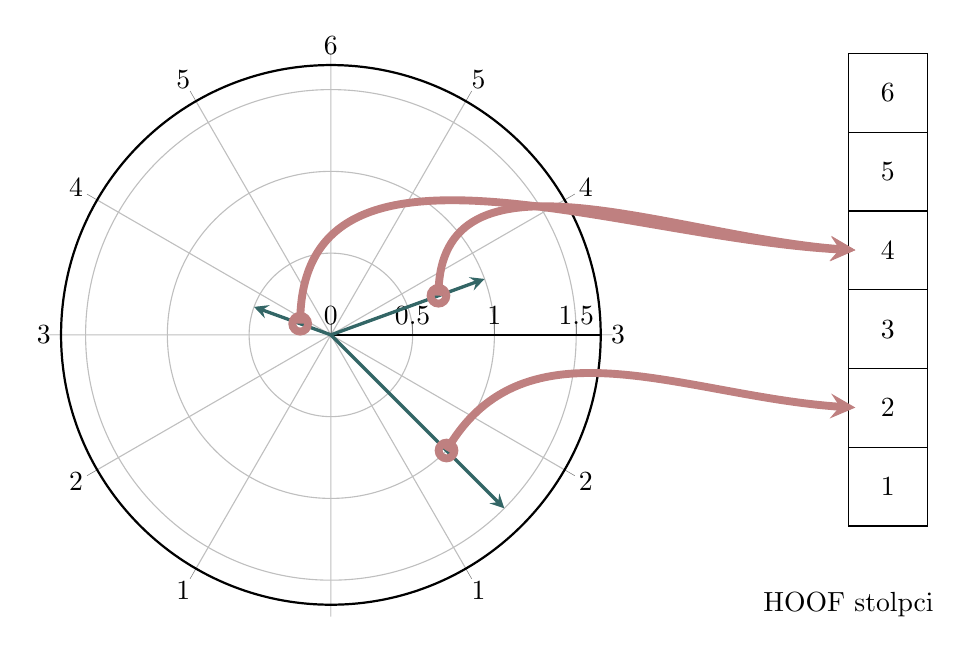
\begin{tikzpicture}
% LAYERS
\pgfdeclarelayer{bg}
\pgfsetlayers{bg,main}

 % LENGTHS
\newcommand{\csl}{5}
\newcommand{\vl}{3}

\begin{pgfonlayer}{bg}
% Coordinate system
\begin{scope}
	\tikzset{vec/.append style = {
    	draw=teal!50!black!80,
        very thick
    }}
	\begin{polaraxis}[hoof plot style]
		\addplot[vec, domain=0:1](20,x);
        \coordinate (v1) at (20, 0.7);
        \addplot[vec, domain=0:1.5](-45,x);
        \coordinate (v2) at (-45, 1);
        \addplot[vec, domain=0:0.5](160,x);
        \coordinate (v3) at (160,0.2);
	\end{polaraxis}
\end{scope}

\begin{scope}[xshift=10cm, yshift=0pt]
	\draw (0,1) rectangle (1,2) node (h1) [midway] {$1$};
    \draw (0,2) rectangle (1,3) node (h2) [midway] {$2$};
    \draw (0,3) rectangle (1,4) node (h3) [midway] {$3$};
    \draw (0,4) rectangle (1,5) node (h4) [midway] {$4$};
    \draw (0,5) rectangle (1,6) node (h5) [midway] {$5$};
    \draw (0,6) rectangle (1,7) node (h6) [midway] {$6$};
    \node at (0,0) {HOOF stolpci};
\end{scope}
\end{pgfonlayer}

\tikzset{show/.style={
	->,
    >=stealth,
    very thick,
    line width=1mm,
    draw=red!50!black!50,
    shorten >=2mm
    }}
\draw [show] (v1) circle (1mm);
\draw [show] (v1) to[out=90, in=180] (h4);
\draw [show] (v2) circle (1mm);
\draw [show] (v2) to[out=60, in=180] (h2);
\draw [show] (v3) circle (1mm);
\draw [show] (v3) to[out=90, in=180] (h4);
\end{tikzpicture}}
\caption[Prikaz določitve histograma HOOF glede na kot vektorja]{Prikaz določitve HOOF histograma glede na kot vektorja optičnega toka $\vec{w}$. Slika prikazuje določitev za $6$ stolpcev.}
\label{fig:hoof-histogram}
\end{figure}




Preslikava intervala~\eqref{eq:interval-kot2} v interval~\eqref{eq:interval-kot} omogoča neodvisnost histograma vzdolž $x$ osi~\cite{chaudhry2009histograms}. Z normiranjem histograma dobimo invariantnost na skalo~\cite{chaudhry2009histograms}. Ker je vsak prispevek vektorja sorazmeren njegovi amplitudi, šumni vektorji nimajo vpliva na obliko histograma~\cite{chaudhry2009histograms}. Posledično lahko določimo histogram za celotno sliko in zato ne potrebujemo segmentacije ali subtrakcije gibajoče se osebe iz ozadja. 

Edini parameter, ki ga moramo določiti za značilke HOOF, je število stolpcev histograma $N_{HOOF}$. Chaudry et al.~\cite{chaudhry2009histograms} pravi, da moramo za dobro delovanje določiti najmanj $30$ stolpcev. 







\subsection{Histogrami absolutnih tokovnih amplitud}\label{sec:hafa}
% Opis dodatnih deskriptorjev
% Kako uporabili nove deskriptorje
Deskriptor HOOF modelira smer gibanja, zato vsebuje le del informacije, ki jo potrebujemo za esetimacijo porabe energije. Ostalo informacijo vsebuje amplituda gibanja, ki jo dobimo z amplitudo vektorja optičnega toka. Idejo deskriptorja za modeliranje amplitude gibanja smo dobili v delu~\cite{pers2010histograms}, kjer so avtorji za opis gibanja uporabili histograme optičnega toka (HOF). Gre za histograme v dveh dimenzijah, ki posebej kvantizirata amplitudo in smer optičnega toka v podregijah slike. 

Vektor optičnega toka $\vec{w}$, ki je opredeljen v poglavju~\ref{sec:hoof}, ima amplitudo določeno na intervalu~\eqref{eq:interval-amp1}. 

\begin{equation}\label{eq:interval-amp1}
	[0, \infty)
\end{equation}


Interval~\eqref{eq:interval-amp1} lahko kvantiziramo po enačbi~\eqref{eq:interval-amp2}. Ta pomeni, da vektorju $\vec{w}$ določimo stolpec $b$, za katerega velja $1 \leq b \leq N_{HAFA}$, pri čemer je $N_{HAFA}$ celotno število stolpcev histograma na podlagi amplitude $\| \vec{w} \|$. S tako kvantizacijo omejimo zgornjo mejo intervala~\eqref{eq:interval-amp1} na parameter histograma $N_{HAFA}$. Ko tak histogram normiramo, ga imenujemo histogram absolutnih tokovnih amplitud (HAFA). Določitev histograma HAFA je prikazana na sliki~\ref{fig:hafa-histogram}.

\begin{equation}\label{eq:interval-amp2}
	\frac{b-1}{N_{HAFA}} \leq \norm{\vec{w}} < \frac{b}{N_{HAFA}}
\end{equation}




\begin{figure}[!htb]
\centering
\resizebox{0.5\columnwidth}{!}{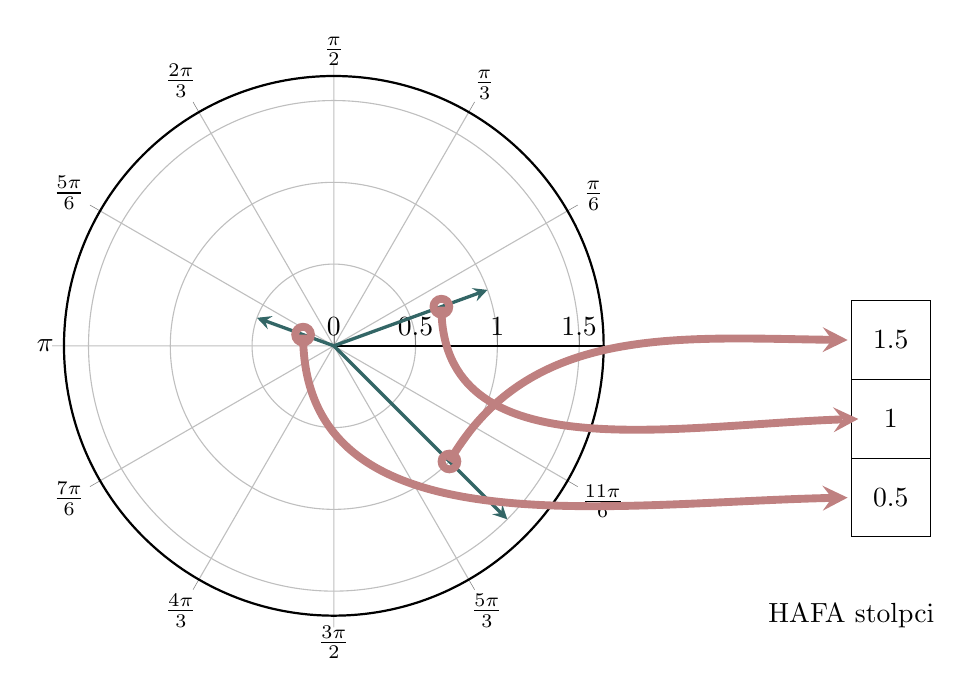
\begin{tikzpicture}
% LAYERS
\pgfdeclarelayer{bg}
\pgfsetlayers{bg,main}

 % LENGTHS
\newcommand{\csl}{5}
\newcommand{\vl}{3}

\begin{pgfonlayer}{bg}
% Coordinate system
\begin{scope}
	\tikzset{vec/.append style = {
    	draw=teal!50!black!80,
        very thick
    }}
	\begin{polaraxis}[polar plot style]
		\addplot[vec, domain=0:1](20,x);
        \coordinate (v1) at (20, 0.7);
        \addplot[vec, domain=0:1.5](-45,x);
        \coordinate (v2) at (-45, 1);
        \addplot[vec, domain=0:0.5](160,x);
        \coordinate (v3) at (160,0.2);
	\end{polaraxis}
\end{scope}

\begin{scope}[xshift=10cm, yshift=0pt]
	\draw (0,1) rectangle (1,2) node (h1) [midway] {$ 0.5$};
    \draw (0,2) rectangle (1,3) node (h2) [midway] {$1$};
    \draw (0,3) rectangle (1,4) node (h3) [midway] {$1.5$};
    \node at (0,0) {HAFA stolpci};
\end{scope}
\end{pgfonlayer}

\tikzset{show/.style={
	->,
    >=stealth,
    very thick,
    line width=1mm,
    draw=red!50!black!50,
    shorten >=2mm
    }}
\draw [show] (v1) circle (1mm);
\draw [show] (v1) to[out=-90, in=180] (h2);
\draw [show] (v2) circle (1mm);
\draw [show] (v2) to[out=60, in=180] (h3);
\draw [show] (v3) circle (1mm);
\draw [show] (v3) to[out=-90, in=180] (h1);
\end{tikzpicture}
}
\caption[Prikaz določitve histograma HAFA glede na velikost vektorja]{Prikaz določitve histograma HAFA glede na velikost vektorja optičnega toka $\vec{w}$. Slika prikazuje določitev za $3$ stolpce.}
\label{fig:hafa-histogram}
\end{figure}



\subsection{Razširitev histogramov za uporabo s prostorskim tokom}
Histograma HOOF in HAFA lahko uporabimo tudi za tridimenzionalni prostorski tok $\vec{\mu}$. Enačbo amplitude~\eqref{eq:amplituda} lahko zamenjamo z enačbo amplitude~\eqref{eq:amplituda-3d} za prostorski tok $\vec{\mu} = \left[\mu_x~\mu_y~\mu_z \right]^\top$.

\begin{equation}
\norm{\vec{\mu}} = \sqrt{\mu_x^2 + \mu_y^2 + \mu_z^2} 
\label{eq:amplituda-3d}
\end{equation}

Smer $\Theta$ določimo s preslikavo vektorja prostorskega toka $\vec{\mu}$ na slikovno ravnino $\varOmega$ po enačbi~\eqref{eq:smer-3d}, saj velja povezava med prostorskim tokom $\vec{\mu}$ in optičnim tokom $\vec{w}$~\eqref{eq:of-sf}.


\begin{equation}
\Theta = \tan^{-1}\left( \frac{\norm{\vec{w}}}{\norm{\vec{\mu}}} \right)
\label{eq:smer-3d}
\end{equation}

Enačbe temeljijo na obrazcih za prehod iz kartezičnih koordinat $(x, ~y, ~z)$ na sferične koordinate $(r,~\phi,~\Theta)$~\cite{bronstein1990math}, pri čemer upoštevamo postavitev koordinatnega sistema po perspektivnem modelu kamere iz poglavja~\ref{sec:model-kamere}. Slika~\ref{fig:sphere} prikazuje sferične koordinate v koordinatnem sistemu kamere, kjer zaradi poenostavitve slikovna ravnina poteka skozi koordinatno izhodišče $\vec{O}$. Za koordinato $r$ velja $r=\norm{\vec{\mu}}$. Za enolično določitev točk prostora velja, da $\Theta$ leži na intervalu $\left[\frac{-\pi}{2},~\frac{\pi}{2}\right]$, $\phi$ pa na intervalu $\left[0,~2\pi\right)$.

\begin{figure}[htb]
	\centering
	\begin{tikzpicture}%[tdplot_main_coords, scale=0.5]
[x={(0.8cm,0.4cm)}, y={(0cm,1cm)}, z={(0.8cm,-0.4cm)}, scale=0.5]

	% Coordinate system
    \coordinate (O) at (0,0,0);
    \coordinate (oo) at (0,0,5);
    \coordinate (y) at (0,5,0);
    \coordinate (z) at (0,0,15);
    \coordinate (x) at (10,0,0);
    \draw [axis, thick] (O) -- (y) node [right] {$y$};
    \draw [axis] (O) -- (z) node [below] {$z$};
    \draw [axis] (O) -- (x) node [below] {$x$};
    \node (izhodisce) [below] at (O) {$\vec{O}$};
   
    
    % delec
    \coordinate (p) at (5,3,10);
    \coordinate (p') at (5,0,10);
    \draw [vec] (O) -- (p) node (r) [midway] {};
    \node (mu) [above] at (p) {$\vec{\mu}$};
    \draw [dash] (5,0,0) node [above] {$X$} -- (p');
    \draw [dash] (0,0,10) node [below] {$Z$} -- (p');
    \draw [dash] (p') -- (p);
    \draw [dash] (O) -- (p') node (pm) [midway] {};
	
	% angle1
	\begin{scope}[canvas is xy plane at z=0]
	\node at (\spherical{5.5}{60}{80})  {$\Theta$};
    \path[clip] (p) -- (O) -- (p');
    \draw[angle=teal] (O) circle (5.5cm);
	\end{scope}
	 
	%angle2
	\begin{scope}[canvas is xz plane at y=0]
	\coordinate (Oc) at (0,0);
	\coordinate (zc) at (0,15);
	\coordinate (pc) at (5,10);
	\path[clip] (pc) -- (Oc) -- node (mc){} (zc);
	\draw[angle=red] (Oc) circle (5cm);
	\node at (\spherical{5.5}{0}{10})  {$\phi$};
	\end{scope}
	    
\end{tikzpicture}
	\caption[Sferične koordinate v koordinatnem sistemu kamere]{Sferične koordinate v koordinatnem sistemu kamere nam omogočajo razširitev histogramov za uporabo s prostorskim tokom.}
	\label{fig:sphere}
\end{figure}

S tako uporabljenimi enačbami za histograme izgubimo informacijo o smeri v histogramu HOOF, saj kota $\phi$ ne upoštevamo. To je sprejemljivo, saj nam mora histogram omogočati neodvisnost v smeri premikanja od leve proti desni~\cite{chaudhry2009histograms}. To pa je ravno kot $\phi$. Po preslikavi prostorskega kota $\vec{\mu}$ na slikovno ravnino je določitev histogramov trivialna. 

\section{Matematični modeli}\label{sec:matematicni-modeli}
Metode strojnega učenja s podpornimi vektorji (SVM) se pogosto uporabljajo za klasifikacijo in regresijo \cite{chang2011a}. Njihova popularnost temelji na visoki uspešnosti generalizacije brez potrebe po predhodnem znanju \cite{chapelle1999support}. Njihova performanca delovanja ni odvisna od števila značilk, saj jih ponavadi uporabljamo v primerih ko ima vhodni prostor značilk $\mathcal{W}^n$ veliko moč $n$. Cilj teh metod je, da generiramo matematični model in ga uporabimo za predikcijo izhoda $y$ \cite{hsu2003practical}. 








\subsection{Linearno ločljiva učna množica}
Imamo učne vzorce $\{ \vec{x}_i, y_i \} \in \mathcal{U}_l$, kjer je $\vec{x}_i \in \mathcal{\Xi}_l \subset \mathbb{R}^n~\forall i = 1, \ldots, l$ vektor značilk oziroma deskriptor in $y_i \in \mathit{\Omega}_l \subset \mathbb{R}~\forall i = 1, \ldots, l$ oznake razredov objektov \cite{chapelle1999support}. Za poenostavitev privzamemo, da imamo samo dva razreda $y_i \in \{-1,1\}$. 

Pri postopku s podpornimi vektorji v splošnem iščemo koeficiente $\vec{w} \in \mathcal{W} \subset \mathbb{R}^m$ ločilnih mej ali \textbf{hiper-ravnin} in prag $b$, ki razmejujejo prostor $\mathbb{R}^n$ tako, da so enako oddaljene od vzorcev $\vec{x}$ iz različnih razredov $\mathcal{C}_i~\forall i= 1, \ldots, p$, kot je prikazano na sliki \ref{fig:svm-locljivo} \cite{chapelle1999support}. Pri tem velja omejitev

\begin{equation}\label{eq:omejitev-ravnine}
	y_i(\vec{w} \vec{x}_i + b) \geq 1, i=1, \ldots, l.
\end{equation}





\begin{figure}[htb]
\centering
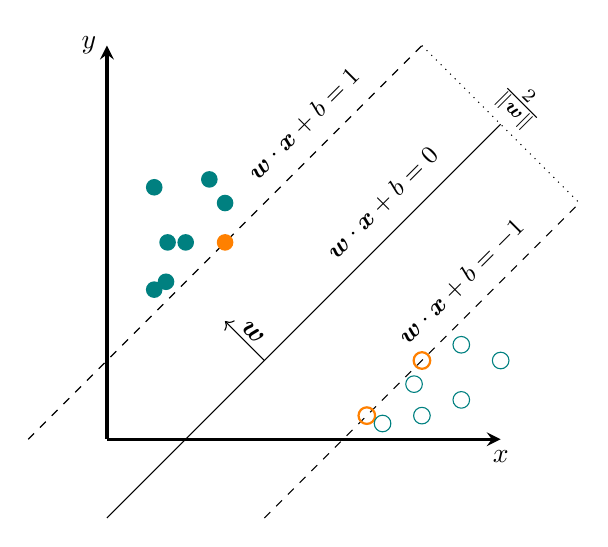
\begin{tikzpicture}[scale=1.0]
	% Draw axes
  \draw [axis] (0,0) -- (0,5) node (yaxis) [left] {$y$};
  \draw [axis] (0,0) -- (5,0) node (xaxis) [below] {$x$};
  % Draw line
  \draw (0,-1) -- (5,4); % y=x-1
  \draw[dashed] (-1,0) -- (4,5); % y=x+1
  \draw[dashed] (2,-1) -- (6,3); % y=x-3
  % Draw labels
  \draw (3.5,3) node[rotate=45,font=\small] 
        {$\vec{w}\cdot \vec{x} + b = 0$};
  \draw (2.5,4) node[rotate=45,font=\small] 
        {$\vec{w}\cdot \vec{x} + b = 1$};
  \draw (4.5,2) node[rotate=45,font=\small] 
        {$\vec{w}\cdot \vec{x} + b = -1$};
  % Draw distance
  \draw[dotted] (4,5) -- (6,3);
  \draw (5.25,4.25) node[rotate=-45] {$\frac{2}{\Vert \vec{w} \Vert}$}; 
  \draw[->] (2,1) -- (1.5,1.5);
  \draw (1.85,1.35) node[rotate=-45] {$\vec{w}$};
  % Draw negative dots
  \fill[orange]   (1.5,2.5)   circle (3pt);
  \fill[teal] (1,2.5)     circle (3pt);
  \fill[teal] (0.75,2)    circle (3pt);
  \fill[teal] (0.6,1.9)   circle (3pt);
  \fill[teal] (0.77, 2.5) circle (3pt);
  \fill[teal] (1.5,3)     circle (3pt);
  \fill[teal] (1.3,3.3)   circle (3pt);
  \fill[teal] (0.6,3.2)   circle (3pt);
  % Draw positive dots
  \draw[orange,thick] (4,1)     circle (3pt); 
  \draw[orange,thick] (3.3,.3)  circle (3pt); 
  \draw[teal]     (4.5,1.2) circle (3pt); 
  \draw[teal]     (4.5,.5)  circle (3pt); 
  \draw[teal]     (3.9,.7)  circle (3pt); 
  \draw[teal]     (5,1)     circle (3pt); 
  \draw[teal]     (3.5,.2)  circle (3pt); 
  \draw[teal]     (4,.3)    circle (3pt); 
    
\end{tikzpicture}
\caption[Prikaz ločevanja vzorcev na razrede s podpornimi vektorji]{Prikaz ločevanja vzorcev na razrede s podpornimi vektorji. Na sliki je prikazan primer ločevanja na dva razreda.}
\label{fig:svm-locljivo}
\end{figure}




Če hiper-ravnina obstaja, pravimo, da je množica $\mathcal{U}_l$ \textbf{linearno ločljiva} \cite{chapelle1999support}. Ker želimo določiti ločilno mejo s čim širšim robom, moramo minimizrati $\|\vec{w}\|^2$, saj je razdalja med mejo in najbližjo točko $\frac{1}{\|\vec{w}\|}$. To naredimo z vpeljavo Lagrangeovih multiplikatorjev $\vec{\alpha} \in \mathcal{A}^i$ in maksimizacijo funkcije \eqref{eq:svm-lagrange} z omejitvijo \eqref{eq:svm-lagrange-omejitev} \cite{chapelle1999support}.

\begin{equation}\label{eq:svm-lagrange}
	\mathcal{L}(\vec{\alpha}) = \sum_{i=1}^l \alpha_i - \frac{1}{2}\sum_{i,j=1}^l \alpha_i\alpha_j y_i y_j \vec{x}_i^\top\vec{x}_j
\end{equation}

\begin{equation}\label{eq:svm-lagrange-omejitev}
	\sum_{i=1}^ly_i\alpha_i = 0, \alpha_i \geq 0; i=1, \ldots, l
\end{equation}

Z rešitvijo maksimizacijskega problema \eqref{eq:svm-lagrange} $\vec{\alpha}^0$ lahko izračunamo optimalne koeficiente \cite{chapelle1999support}:

\begin{equation}
	\vec{w}_0 = \sum_{i=1}^l \alpha_i^0 y_i \vec{x}_i.
\end{equation}

Učnim vzorcem, za katere so $\alpha_i^0 > 0$ pravimo \textbf{podporni vektorji} \cite{chapelle1999support}.









\subsection{Linearno neločljiva učna množica}
Pri linearno neločjivi učni množici $\mathcal{U}_l$ uvedemo dodaten vektor spremenljivk $\vec{\xi} \in \mathit{\Lambda}^i$ in rešujemo optimizacijski problem \eqref{eq:svm}, kjer je $C>0$ regularizacijski parameter napake in $b$ prag \cite{chapelle1999support}. Večji $C$ pomeni manjšo dopustnost napak. 

\begin{equation}\label{eq:svm}
\begin{aligned}
\min_{\vec{w}, b, \vec{\xi}} &~ \left\{ \frac{1}{2} \vec{w}^\top\vec{w} + C \sum_{i=1}^l\xi_i \right\}\\
    \mathrm{z~omejitvijo} &~ y_i \left( \vec{w}^\top \vec{x}_i + b \right) \geq 1 - \xi_i,~ 
    \xi_i \geq 0
\end{aligned}	
\end{equation}








\subsection{Funkcije jedra}
V primeru, ko učnih vzorcev ne moremo razmejiti brez napak v linearno hiper-ravnino jih lahko preslikamo v več razsežni prostor z nelinearno preslikavo $\phi: \mathcal{\Xi} \subset \mathbb{R}^n \to \mathcal{\Mu} \subset \mathbb{R}^m, n < m$, kjer lahko postanejo linearno separabilni \cite{chapelle1999support,boughorbel2005generalized}.Tako v enačni \eqref{eq:svm-lagrange} namesto $\vec{x}_i^\top\vec{x}_j$ uporabimo $\phi(\vec{x_i})^\top\phi(\vec{x_j})$ Preslikovanju vzorcev v m-razsežni prostor se lahko znebimo s t.i. \textbf{ukano jedra} (angl. Kernel trick), kjer uporabimo implicitno preslikavo $K: \mathcal{\Xi} \times \mathcal{\Xi} \to \mathbb{R}$ \cite{boughorbel2005generalized}. V skladu z Mercerjevim izrekom mora biti $K(\vec{x}_i,\vec{x}_j)$ simetrična in pozitivna funkcija. Takrat obstaja preslikava $\phi$ tako da velja $K(\vec{x_i}, \vec{x_j}) = \phi(\vec{x}_i)^\top\phi(\vec{x}_j)$.


\subsubsection{Jedro radialnih baznih funkcij}{
Jedro radialnih baznh funckij (RBF) ima naslednjo obliko z enim hiper-parametrom $\gamma$ \cite{hsu2003practical}:

\begin{equation} \label{eq:rbf-kernel}
		K_{RBF}(\vec{x_i}, \vec{x_j}) = e^{
        	-\gamma 
        	\begin{Vmatrix}
        		\vec{x_i} - \vec{x_j}
        	\end{Vmatrix}^2
        }
\end{equation}

Avtorji v \cite{hsu2003practical} zagovarjajo, da pri učenju najprej poskusim z RBF jedrom. Prvi argument je, da to jedro ne vpliva na kompleksnost modela, saj moramo izbrati le en dodaten parameter $\gamma$. Kot drugo, imamo z njim manj numeričnih težav, saj se njegova vrednost giblje na intervalu $(0, 1]$ \cite{hsu2003practical}. 



\subsubsection{Jedro preseka generaliziranih histogramov}
Jedro preseka generaliziranih histogramov (GHI) je uporaben, ko imamo deskriptorje definirane kot histograme. Določen z enačbo \eqref{eq:ghi-kernel}, kjer je hiper-parameter $\beta \geq 0$, $m$ pa je število stolpcev histogramov $\vec{x}$ in $\vec{x}'$ \cite{boughorbel2005generalized}.

\begin{equation}\label{eq:ghi-kernel}
K_{GHI}(\vec{x}, \vec{x}') = \sum_{i=1}^m min\left\{ \left| x_i \right|^\beta, \left|  x_i' \right| \right\}
\end{equation}

Po \cite{boughorbel2005generalized} je prednost uporabe GHI jedra ta, da so meje invariantne na skaliranje prostora značilk, zato ne potrebujemo dodatne optimizacije skalirnega hiper-parametra. Optimalna vrednosti hiper-parametra je okoli $\beta=0.25$.

%\subsubsection{linear}






\subsection{Predprocesiranje}
\subsubsection{Skaliranje značilk}

Po \cite{hsu2003practical} je skaliranje značilk pred uporabo SVM zelo pomembno. S skaliranjem se znebimo dejstva, da značilke, definirane na večjem intervalu bolj vplivajo na rezultat, kot značilke z manjšim intervalom. Prav tako se s skaliranjem znebimo numeričnih težav med učenjem. Avtorji \cite{hsu2003practical} zato predlagajo skaliranje na intervalih $[-1, 1]$ ali $[0, 1]$.







\subsubsection{Optimizacija SVM parametrov}\label{sec:optimizacija-svm-parametrov}

Ker a priori ne poznamo najboljših parametrov postopka SVM in hiper-parametrov funkcij jedra, jih moramo optimizirati \cite{hsu2003practical}. S tem zagotovimo najboljše delovanje metode na naših podatkih. Za optimizacijo lahko uporabljamo mrežno iskanje s križno validacijo.  Pri mrežnem iskanju izračunamo predikcije za kombinacijo parametrov in jih evaluiramo s križno validacijo \cite{hsu2003practical}. Izberemo tisto kombinacijo parametrov, s katero smo dobili najboljšo natančnost. 

Dobro je, če kombinacije parametrov izbiramo po eksponentni funkciji z osnovo $2$, saj s tem zagotovimo širok razpon iskanja \cite{hsu2003practical}. Iskanje optimalnih parametrov lahko pohitrimo z uporabo grobega in finega iskanja. Z grobim iskanjem omejimo območje iskanja za fino iskanje \cite{hsu2003practical}. S finim iskanjem pa dejansko optimiziramo parametre.






\subsection{Postopki SVM}
\subsubsection{Razvrščevalnik C-SVC}

Razvrščevalnik rešuje problem \cite{chang2011a}:

\begin{equation}\label{eq:c-svc}
\begin{aligned}
\min_{\vec{\alpha}} &~ \left\{ \frac{1}{2} \vec{\alpha}^\top Q \vec{\alpha} - \vec{e}^\top \vec{\alpha} \right\}\\
    \mathrm{z~omejitvijo} &~ \vec{y}^\top \vec{\alpha} = 0,~ 
    0 \geq \alpha_i \geq C, i=1, \ldots, l.
\end{aligned}	
\end{equation}

$\vec{e}$ je vektor enic. $Q$ je pozitivna semidefinitna matrika s členi $Q_{ij} = y_i y_jK(\vec{x}_i,\vec{x}_j)$, kjer je $K(\vec{x}_i,\vec{x}_j)$ funkcija jedra. $\vec{\alpha}$ so Lagrangeovi multiplikatorji in $C>0$ je regularizacijski parameter \cite{chang2011a}.








\subsubsection{Regresija \texorpdfstring{$\epsilon$}{e}-SVR}

Za uporabo SVM pri regresiji uvedemo dodatni vektor spremenljivk $\vec{\xi^+}$. Primarni problem regresije $\epsilon$-SVR je  tako \cite{chang2011a}:

\begin{equation}\label{eq:e-svr-primal}
\begin{aligned}
\min_{\vec{w}, b, \vec{\xi}, \vec{\xi}^+} &~ \left\{ \frac{1}{2} \vec{w}^\top\vec{w} + C \sum_{i=1}^l\xi_i + C \sum_{i=1}^l\xi_i^+ \right\}\\
    \mathrm{z~omejitvijo} &~ y_i \left( \vec{w}^\top \vec{x}_i + b \right) \geq \epsilon - \xi_i,\\
    &~  y_i \left( \vec{w}^\top \vec{x}_i + b \right) \leq \xi_i^+ - \epsilon, \\
    &~  \xi_i,\xi_i^+ \geq 0, i=1, \ldots, l,
\end{aligned}	
\end{equation}

kjer je $C>0$ regresijski parameter in $\epsilon > 0$ parameter kriterijske funkcije. Z njim določujemo toleranco do napak.

Sekundarni problem se glasi \cite{chang2011a}:

\begin{equation}\label{eq:e-svr-dual}
\begin{aligned}
\min_{\vec{\alpha}, \vec{\alpha}^+} &~ \left\{ \frac{1}{2} (\vec{\alpha} - \vec{\alpha^ +})^\top Q (\vec{\alpha} - \vec{\alpha}^+) +\right. \\
&~ \left.\epsilon \sum_{i=1}^l\left( \alpha_i + \alpha_i^+ \right) + \sum_{i=1}^l y_i\left( \alpha_i - \alpha_i^+ \right) \right\}\\
    \mathrm{z~omejitvijo} &~ 
    \vec{e}^\top \left(\vec{\alpha} - \vec{\alpha^+} \right) = 0,\\
    &~ 0 \geq \alpha_i, \alpha_i^+ \geq C, i=1, \ldots, l.
\end{aligned}	
\end{equation}

$Q$ je matrika s z elementi $Q_{ij} = KK(\vec{x}_i,\vec{x}_j)$.





\subsubsection{Regresija \texorpdfstring{$\nu$}{nu}-SVR}

Pri regresiji $\nu$-SVR uporabljamo dodatni parameter $\nu \in (0, 1]$, s katerim kontroliramo razmerje števila podpornih vektorjev. Ostali parametri so enaki kot pri $\epsilon$-SVR, le da tu $\epsilon$ postane spremenljivka \cite{chang2011a}. Primarni problem se glasi:

\begin{equation}\label{eq:nu-svr-primal}
\begin{aligned}
\min_{\vec{w}, b, \vec{\xi}, \vec{\xi}^+, \epsilon} &~ \left\{ \frac{1}{2} \vec{w}^\top\vec{w} + C (\nu\epsilon + \frac{1}{l}\sum_{i=1}^l\xi_i + \xi_i^+ \right\}\\
    \mathrm{z~omejitvijo} &~ 
    y_i \left( \vec{w}^\top \vec{x}_i + b \right) \geq \epsilon - \xi_i,\\
    &~  y_i \left( \vec{w}^\top \vec{x}_i + b \right) \leq \xi_i^+ - \epsilon, \\
    &~  \xi_i,\xi_i^+ \geq 0, i=1, \ldots, l, \epsilon \geq 0.
\end{aligned}	
\end{equation}

Sekundarni problem opišemo z \cite{chang2011a}:

\begin{equation}\label{eq:nu-svr-dual}
\begin{aligned}
\min_{\vec{\alpha}, \vec{\alpha}^+} &~ \left\{ \frac{1}{2} (\vec{\alpha} - \vec{\alpha^ +})^\top Q (\vec{\alpha} - \vec{\alpha}^+) + \vec{y}^\top \left( \alpha_i - \alpha_i^+ \right) \right\}\\
    \mathrm{z~omejitvijo} &~ 
    \vec{e}^\top \left(\vec{\alpha} - \vec{\alpha^+} \right) = 0,~ 
    \vec{e}^\top \left(\vec{\alpha} + \vec{\alpha^+} \right) \leq C\nu,\\
    &~ 0 \geq \alpha_i, \alpha_i^+ \geq C/l, i=1, \ldots, l.
\end{aligned}	
\end{equation}


\section{Sledilnik}
% tracker
% Zakaj smo uporabili sledilnik
% Na katere sledilnike smo ciljali 
% Primerjava sledilnikov
% Naši eksperimenti kateri je boljši
%
Gibanje objektov v prostoru zaznamo kot temporalno spreminjanje slike. Ta lastnost nam omogoča izluščenje koristnih informacij, kot je identifikacija objektov na podlagi karakteristike gibanja, določevanje njihove pozicije in ugotavljanje kaj se v sceni dogaja \cite{forsyth2002computer}. Forsyth et. al \cite{forsyth2002computer} sledenje opiše kot postopek, s katerim sklepamo o gibanju objektov glede na zaporedje slik. Problem sledenja v računalniškem vidu še ni v celoti rešljiv, saj obstaja veliko faktorjev, ki otežujejo delo sledilnikov \cite{danelljan2014adaptive}. Med njimi sodijo okluzija objekta, ki mu sledimo, razne geometrijske deformacije in zamegljenost zaradi hitrega gibanja, temporalno spreminjanje osvetljenosti, šum iz ozadja ter variacije v skali. 

Sledilnike delimo v glavnem na dva pristopa: generativne in diskriminativne metode \cite{danelljan2014adaptive}. Pri \textbf{generativnih metodah} iščemo področja, ki so najbolj podobna modelu tarče. \textbf{Diskriminativne metode} predstavljajo binarni problem razvrščanja, saj pri njih želimo določiti mejo med tarčo in ozadjem. Slednjo metodo uporabljamo pri sledenju z detekcijo, ki daje najboljše rezultate \cite{danelljan2014adaptive}. Glavna ideja takega sledenja je sprotno učenje razvrščevalnika s trenutnim vzorcem tarče. Sledi korak detekcije tarče na naslednji sliki zaporedja z razvrščevalnikom in vizualno predstavitvijo tarče, ki smo se jo naučili skozi čas.






\subsection{Zmanjševanje merilne napake}

Položaj subjektov, ki jih opazujemo, ni mogoče omejiti zunaj skrbno urejene laboratorijske postavitve, saj uporabljamo tokovna polja brez kakršnekoli predpostavke o postavitvi skeleta in brez kakršnih koli dodatnih omejitev. V takem primeru bi bila prevladujoča komponenta histogramov šum. Zato moramo uvesti algoritem za sledenje, da lokaliziramo položaj opazovanega subjekta v koordinatnem sistemu slike.

Z uporabo sledilnika dobimo realnejšo sliko meritve, saj se znebimo šuma iz ozadja (premikanja slikovnih elementov, ki niso del tarče). Izognemo se napaki merjenja zaradi šuma CCD senzorja in premikanja drugih objektov. To so lahko razni predmeti (žoge, loparji, itd.) ali druge osebe. Brezkontaktnemu merilnemu instrumentu tako dodamo širšo uporabno vrednost, saj ga v nasprotnem primeru ne bi mogli uporabljati v ekipnih športih in športih z žogo. 

Zaradi uporabe optičnega in prostorskega toka pri določevanju modela gibanja nam merilno napako povzroča tudi premikanje kamere. S premikanjem kamere povzročimo relativno premikanje objektov glede na koordinatni sistem kamere, četudi so ti glede na referenčni koordinatni sistem v prostoru pri miru. Tega problema se lahko znebimo z uporabo sledilnika. 

Predpostavimo, da imamo idealni sledilnik in enako definicijo in omejitve kamere, masnega delca, slike delca in osvetlitve kot v poglavju \ref{sec:opticni-tok}. Idealni sledilnik v vsaki sliki zaporedja najde sliko delca $\vec{q}$ in posamezno sliko v zaporedju obreže tako, da je težišče tarče vedno v centru obrezane slike. Ne glede na gibanje kamere, bo pozicija slike delca $\vec{q}$ vedno v centru slikovne ravnine. Gibanje kamere zato ne bo vplivalo na optični tok $\mathcal{O}$.



\subsection{Sledilnik za optični tok} 
Sledilnik temelji na delu \cite{danelljan2014adaptive}, kjer izboljšajo originalni KCF sledilnik iz dela \cite{henriques2012exploiting} z uporabo barvnih značilk. KCF sledilnik sodi med metode sledenja z detekcijo. Njegovo delovanje je prikazano na sliki \ref{fig:diagram-kcf}.

\begin{figure}[htb]
	\centering
	\resizebox{\columnwidth}{!}{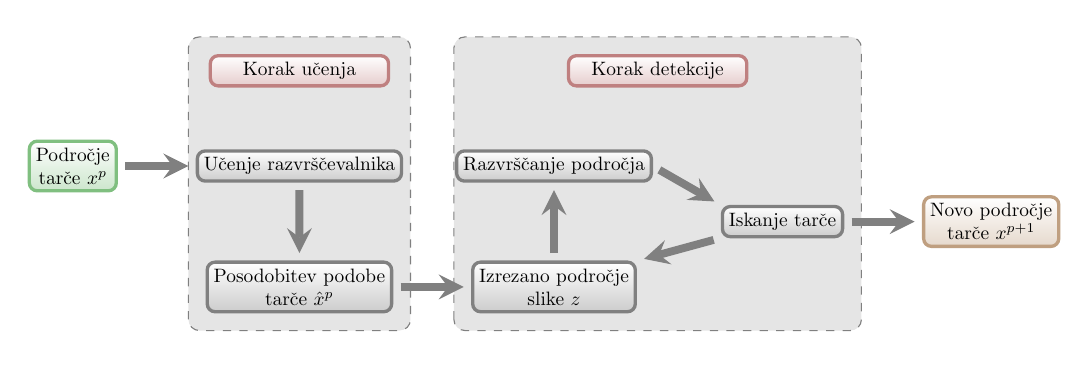
\begin{tikzpicture}
% LAYERS
\pgfdeclarelayer{bg}
\pgfsetlayers{bg,main}
\tikzset{
    between/.style args={#1 and #2}{
         at = ($(#1)!0.5!(#2)$)
    }
}

% NODES
\node (slika) [input] at (0,0) {Področje\\tarče $x^{p}$};
\node (ucenje) [block, right= of slika] {Učenje razvrščevalnika};
\node (tarca) [block, below= of ucenje] {Posodobitev podobe\\tarče $\hat{x}^p$};


\node (podrocje) [block, right=1cm of tarca] {Izrezano področje\\slike $z$};
\node (razvrscanje) [block, above= of podrocje] {Razvrščanje področja};
\node (prcenter) [between=razvrscanje.south and podrocje.north] {};
\node (iskanje) [block, right=2cm of prcenter] {Iskanje tarče};


\node (center) [between= podrocje.west and iskanje.east] {};
\node (kd) [title, above=2cm of center] {Korak detekcije};

\coordinate (c) at ( ucenje.center |- kd);
\node (ku) [title] at (c) {Korak učenja};


\node (rezultat) [output, right= of iskanje] {Novo področje\\ tarče $x^{p+1}$};

% arrows
\draw [arrow] (slika) -- (ucenje);
\draw [arrow] (ucenje) -- (tarca);
\draw [arrow] (tarca) -- (podrocje);
\draw [arrow] (podrocje) -- (razvrscanje);
\draw [arrow] (razvrscanje.east) -- (iskanje.north west);
\draw [arrow] (iskanje.south west) -- (podrocje.north east);
\draw [arrow] (iskanje) -- (rezultat);

\begin{pgfonlayer}{bg}
	\node (ltop) [above = 1mm of ku] {};
	\node (lleft) [left = 1mm of tarca] {};
	\node (lbottom) [below= 1mm of tarca] {};
    \node (lright) [right= 1mm of tarca] {};
  	\node (l0) [] at ( lbottom -| lleft) {};
    \node (l1) [] at (ltop -| lright) {};
    \path[background] (l0) rectangle (l1);
    
    \node (rtop) [above = 1mm of kd] {};
    \node (rright) [right = 1mm of iskanje] {};
    \node (rbottom) [below = 1mm of podrocje] {};
    \node (rleft) [left = 1mm of podrocje] {};
    \node (r0) at (rbottom -| rleft) {};
    \node (r1) at (rtop -| rright) {};
    \path [background] (r0) rectangle (r1);
\end{pgfonlayer}
\end{tikzpicture}}
	\caption[Diagram KCF sledilnika]{Diagram KCF sledilnika.}
	\label{fig:diagram-kcf}
\end{figure}


\paragraph{Korak učenja.}
Na področju tarče $x$ velikosti $M \times N$, vsakemu slikovnemu elementu pripada vrednost Gaussove funkcije $y$. Ob času $p$ poznamo $\mathcal{X}^p = \{x^j: j=1,\ldots,p\}$ področij tarče. Razvrščevalnik učimo z minimizacijo funkcije \eqref{eq:classifier-function}, ki predstavlja uteženo srednjo kvadratično napako čez področja $\mathcal{X}^p$, pri čemer je vsako področje uteženo s konstanto $\beta_j \geq 0$. $\phi$ predstavlja neliearno preslikavo v več razsežni prostor, za katero lahko uporabimo implicitno preslikavo ali funkcijo jedra $K$. V KCF sledilniku se uporablja Gaussovo RBF jedro \eqref{eq:kcf-gauss}. Konstanta $\lambda \geq 0$ je regularizacijski parameter.

\begin{equation}
\begin{aligned}
\epsilon &= \sum_{j=1}^p \beta_j \left( 
	\sum_{m,n} \left| \langle \phi\left(x_{m,n}^j \right), w^j \rangle - y^j(m,n) \right|^2
    + \lambda \langle w^j, w^j \rangle
\right), \\
w^j &= \sum_{k,l} a(k,l) \phi\left(x_{k,l}^j  \right)
\end{aligned}
\label{eq:classifier-function}
\end{equation}

V enačbi \eqref{eq:kcf-gauss} je $\mathcal{F}$ operator diskretne Fourierove transformacije (DFT). Velike začetnice spremenljivk predstavljajo njihove DFT. Tako je $X = \mathcal{F}\{ {x} \}$ DFT področja $x$. $\sigma$ je hiperparameter jedra.

\begin{equation}
K_{RBF}({x}, {x}') = \mathrm{e}^{-\frac{1}{\sigma^2}\left(
	||{x}||^2 + ||{x}'||^2 - 2 \mathcal{F}^{-1}\left\{ {X} {X}' \right\}
\right)}
\label{eq:kcf-gauss}
\end{equation}

Funkcijo \eqref{eq:classifier-function} minimiziramo s koeficientom \eqref{eq:classifier-a}.  $Y^p = \mathcal{F}\{y^p\}$ je DFT gaussove funkcije in $U_x^p = \mathcal{F}\{ K(x_{m,n}^p, x^p) \}$ je DFT jedrne funkcije $K$. $\gamma$ je parameter učenja.

\begin{equation}
A^p = \mathcal{F}\{a^p\} =  \frac{(1- \gamma) A_N^{p-1} + \gamma Y^p U_x^p}
{(1- \gamma)A_D^{p-1} + \gamma U_x^p\left( U_x^p + \gamma \right)}
\label{eq:classifier-a}
\end{equation}

Naučeno vizualno podobo tarče $\hat{x}^p$ ob času $p$ posodobimo z enačbo \eqref{eq:training-target}.

\begin{equation}
\hat{x}^p = (1 - \gamma) \hat{x}^{p-1} + \gamma x^p
\label{eq:training-target}
\end{equation}


\paragraph{Korak detekcije.}
Pri detekciji najprej izrežemo področje $z$ velikosti $M \times N$ na novi sliki. Nato izračunamo rezultate detekcije po enačbi \eqref{eq:detection-score}, kjer je $U_z = \mathcal{F}\left\{ K\left( z_{m,n}, \hat{x}^{p}  \right) \right\}$ DFT izhoda jedrne funkcije področja $z$.

\begin{equation}
\hat{y}^{p + 1} = \mathcal{F}^{-1}\left\{ A U_z \right\}
\label{eq:detection-score}
\end{equation}

Pozicijo tarče nato dobimo s tisto translacijo, ki maksimizira rezultat detekcije $\hat{y}^{p+1}$.












\subsection{Sledilnik za prostorski tok}
Jedro sledilnika temelji na KCF sledilniku za optični tok iz dela \cite{henriques2015high}. Pri tem uporabljajo jedrno funkcijo \eqref{eq:kcf-gauss}. Model tarče je predstavljen z vektorjem značilk, ki je sestavljen iz histograma orientiranih gradientov (HOG) barvne slike in HOG histograma globinske slike. Diagram sledilnika je prikazan na sliki \ref{fig:diagram-dskcf}.

\begin{figure}[htb]
	\centering
	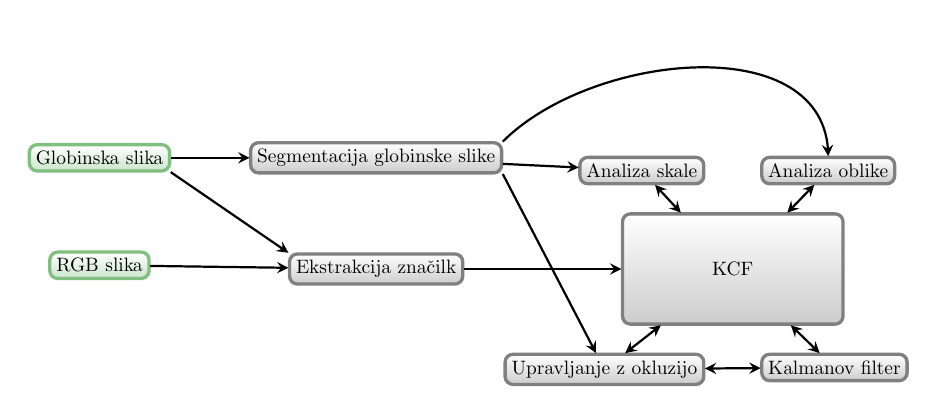
\begin{tikzpicture}
\node (depth) [input] at (0,0) {Globinska slika};
\node (rgb) [input, below= of depth] {RGB slika};
\node (segment) [block, minimum width=1cm, right= of depth] {Segmentacija globinske slike};
\node (feature) [block, below= of segment] {Ekstrakcija značilk};
\node (kcf) [block, minimum width=4cm, minimum height=2cm, right=2cm of feature] {KCF};
\node (scale) [block, above left=5mm of kcf.north] {Analiza skale};
\node (shape) [block, above right=5mm of kcf.north] {Analiza oblike};
\node (occlusion) [block, below left=5mm of kcf.south] {Upravljanje z okluzijo};
\node (kalman) [block, below right=5mm of kcf.south] {Kalmanov filter};

% arrows
\draw [vec] (depth) -- (segment);
\draw [vec] (rgb) -- (feature);
\draw [vec] (depth.south east) -- (feature.north west);

\draw [vec] (segment) -- (scale);
\draw [vec] (segment.north east) to[out=45, in=90] (shape.north);
\draw [vec] (segment.south east) -- (occlusion);

\draw [vec] (feature) -- (kcf);

\draw [vec, <->] (scale) -- (kcf);
\draw [vec, <->] (shape) -- (kcf);
\draw [vec, <->] (occlusion) -- (kcf);
\draw [vec, <->] (kalman) -- (kcf);
\draw [vec, <->] (occlusion) -- (kalman);
\end{tikzpicture}
	\caption[Diagram DS-KCF sledilnika]{Diagram DS-KCF sledilnika. Diagram je povzet po \cite{hannuna2016ds}.}
	\label{fig:diagram-dskcf}
\end{figure}

V DS-KCF sledilniku Najprej segmentirajo globinsko sliko na področja podobne globine s pomočjo rojenja \cite{hannuna2016ds}. S tem pridobijo relevantne značilke globinske distribucije. 

S pomočjo globinske distribucije izračunajo spremembe v skali glede na začetno srednjo vrednost globine tarče in jih uporabijo za posodobitev modela tarče. Posodobitev poteka, ko dobijo novo estimacijo pozicije tarče. Pri tem uporabljajo interpolacijo ali decimacijo v frekvenčnem prostoru \cite{hannuna2016ds}.

V istem času ko sledilnik računa spremembe v skali se globinska distribucija uporabi tudi za detekcijo okluzij. Kadar sledilnik detektira, da je prišlo do okluzije se model tarče ne posodobi \cite{hannuna2016ds}. Pri določevanju okluzije sledilnik uporablja Kalmanov filter, s katerim sledi centru tarče in objekta, ki povzroča okluzijo. V \cite{hannuna2016ds} uporabljajo linearni model konstantne hitrosti.  

Na koncu sledijo popravki zaradi sprememb oblike objekta. Popravki temeljijo na razmerju stranic začetnega pravokotnika modela tarče \cite{hannuna2016ds}. Sledilnik model tarče popravi vedno tako, da razmerje stranic ostaja konstantno.






\section{Filtriranje in glajenje}\label{sec:filtri}
%Filtri so zelo pomembni pri procesiranju signalov \cite{smith1997scientist}. V našem delu jih uporabljamo za izločitev šuma izhodnih podatkov razvrščevalnika. 
Vhodne podatke obdelujemo, bodisi z optičnim tokom ali prostorskim tokom, za vsako sliko video sekvence. Med slikami ne uporabljamo nobene informacije, kar rezultira v oceno porabe energije z veliko šuma. Smiselno je, da zagotovimo časovno kontinuiteto bodisi s filtriranjem ali glajenjem rezultatov porabe energije.

Izbrani filtri izhajajo iz družine filtrov tekočega povprečja, saj so ti najbolj optimalni za zmanjševanje šuma \cite{smith1997scientist}. Splošna enačba filtra tekočega povprečja je \eqref{eq:filter-tekocega-povprecja}, kjer je $x(i)$ i-ti vzorec vhodnega signala, $y(i)$ i-ti vzorec izhodnega signala in $M$ število vzorcev, ki jih uporabimo za filtriranje ali drugače, širina jedra filtra \cite{smith1997scientist}.

\begin{equation}
y(i) = \frac{1}{M} \sum_{j=0}^{M-1} x(i + j)
\label{eq:filter-tekocega-povprecja}
\end{equation}

Prvi filter, ki je bil testiran, je Kalmanov filter. Zaradi slabih rezultatov in težav pri modeliranju hitrih sprememb porabe energije, ki so v številnih športih norma, smo prešli na Gaussov filter (glajenje), kar je dalo zadovoljive rezultate. Ker pridobivamo rezultate v absolutnem realnem času, zamuda, ki jo povzroča Gaussovo glajenje, ni kritična. Oba filtra sta podrobneje opisana v nadaljevanju.

%digitalni filtri so zelo pomemnbi pri digitalnem procesiranju signalov. filtre uporabljamo za dve stvari: signal separation and signam restoration. Prva se uporablja ko imamo signal ki je kontaminiran z interferenco, šumom ali drugimi signali. 

%signal restoration se uporablja ko je bil signal distorted in some way recimo debluring of an image.

%vsak filter im a impulze resonse step response in frekvenčni odziv. filter implementiramo tako da uporabmo konvolucijo z vhodnim signalom. 

%moving average filters
%optimalen za reducing random noise while retaining a sharp step response. najboljši za signale v časovnem prostoru.  -> gaussov filter -> frekvenčni odziv ravno tako gaussian  

\subsection{Digitalni Kalmanov filter}\label{sec:kalmanov-filter}
Kalmanov filter je sestavljen iz modela gibanja, merilnega modela in algoritma s katerim izračunamo novo stanje modela gibanja \cite{trucco1998introductory}.

\subsubsection{Model gibanja}
Gibanje modeliramo z vektorjem stanj $\vec{x}(k)$ na koraku $k$ \cite{trucco1998introductory}. Vektor stanj je predstavljen v enačbi \eqref{eq:vektor-stanj}. Za stanja si ponavadi izberemo tiste spremenljivke gibanja $s_i(k) \forall i = 1,2,\ldots \land k = 0, 1,\ldots$, ki jih opazujemo (npr. pozicija, hitrost, pospešek).

\begin{equation}
\vec{x}(k) = \begin{bmatrix}
					s_1(k) & s_2(k) & \ldots
\end{bmatrix}^\top
\label{eq:vektor-stanj} 
\end{equation}


Model gibanja je vektorska enačba \eqref{eq:model-gibanja}, ki govori o razvoju modela gibanja skozi diskretni čas $k = 0,1,\ldots$ \cite{trucco1998introductory}. Diskretni čas oziroma koraki morajo biti dovolj majhni, da zajamemo dinamiko sistema. $\vec{A}$ je matrika prehajanja stanj in $\vec{G}$ matrika vhodnih parametrov $\tilde{s}_i \forall i = 1,2,\ldots$ v vektorju $\vec{u}(k)$ \eqref{eq:vhodni-parametri}. 



\begin{equation}
\vec{x}(k) = \vec{A} \vec{x}(k-1) + \vec{G} \vec{u}(k)
\label{eq:model-gibanja}
\end{equation}

\begin{equation}
\vec{u}(k) = \begin{bmatrix}
					\tilde{s}_i(k) & \tilde{s}_i(k) & \ldots
			\end{bmatrix}^\top 
\label{eq:vhodni-parametri}
\end{equation}

$\vec{w}(k-1)$ predstavlja Gaussov šum $\mathcal{N}$ modela gibanja s srednjo vrednostjo $0$ in kovariančno matriko $\vec{Q}$, kot je prikazano v enačbi \eqref{eq:sum-modela-gibanja} \cite{trucco1998introductory}.

\begin{equation}
 \vec{w}(k) \sim \mathcal{N}\left(0,\vec{Q}\right)
 \label{eq:sum-modela-gibanja}
\end{equation}

Modeliranje šuma je ekvivalentno določevanju uteži upoštevanja modela v Kalmanovem algoritmu. Večji je šum, večja je negotovost modela, zato bo njegov vpliv na določitev novega stanja manjši \cite{trucco1998introductory}.


\subsubsection{Merilni model}
Pri Kalmanovemu filtriranju predvidevamo, da ob vsakem časovnem trenutku dobimo meritev stanja $\vec{z}(k)$, ki je, realno gledano, pošumljena z Gaussovim šumom \cite{trucco1998introductory}. Merilni model lahko predstavimo z vektorsko enačbo \eqref{eq:merilni-model}, kjer je $\vec{H}$ merilna matrika in $\vec{\nu}(k)$ vektor Gaussovega šuma $\mathcal{N}$ s srednjo vrednostjo $0$ in kovariančno matriko $\vec{R}$ \eqref{eq:sum-merilnega-modela}.


\begin{equation}
 \vec{z}(k) = \vec{H} \vec{x}(k) + \vec{\nu}(k)
 \label{eq:merilni-model}
\end{equation}

\begin{equation}
\vec{\nu}(k) \sim \mathcal{N} \left( 0, \vec{R} \right)
\label{eq:sum-merilnega-modela}
\end{equation}


Tako kot pri modelu gibanja, tudi tu z modeliranjem šuma vnašamo določeno stopnjo negotovosti, ki vpliva na upoštevanje modela pri izračunu novega stanja \cite{trucco1998introductory}.


\subsubsection{Algoritem}
S Kalmanovim algoritmom želimo čimbolj natančno določiti naslednjo oceno stanja sistema $\hat{\vec{x}}(k+1)$, pri čemer uporabimo trenutno meritev $\vec{z}(k)$ in trenutno oceno stanja $\hat{\vec{x}}(k)$ \cite{trucco1998introductory}. 

Jedro algoritma Kalmanovega filtra temelji na izračunavanju kovariančne matrike stanja $\vec{P}$ in matrike ojačanja filtra $\vec{K}$ \cite{trucco1998introductory}. Kovariančna matrika stanja predstavlja oceno vnosa napake zaradi šumnih modelov. Predstavlja šum celotnega sistema. Z ojačanjem določimo, kaj bolj vpliva na novo oceno stanja. Ali trenutna ocena stanja, ali trenutna meritev.

Algoritem lahko razdelimo na tri področja, in sicer: predikcijo, inovacijo in korekcijo \cite{trucco1998introductory}.

\paragraph{Predikcija}
V predikciji določimo trenutno oceno stanja $\hat{\vec{x}}^-(k)$ po enačbi \eqref{eq:ocena-stanja} in a priori kovariančno matriko stanja $\vec{P}^-(k)$ po enačbi \eqref{eq:apriori-p}.

\begin{equation}
	\hat{\vec{x}}^-(k) = \vec{A} \hat{\vec{x}}(k-1) + \vec{G} \vec{u}(k)
    \label{eq:ocena-stanja}
\end{equation}

\begin{equation}
	\vec{P}^-(k) = \vec{A} \vec{P}(k-1) \vec{A}^\top + \vec{Q}
    \label{eq:apriori-p}
\end{equation}

\paragraph{Inovacija}
V koraku inovacije izberemo trenutno meritev $\vec{z}(k)$ iz nabora meritev. Merilno napako $\vec{e}$ določimo po enačbi \eqref{eq:napaka}, kjer drugi člen predstavlja oceno meritve. Kovarianco inovacije $\vec{S}$ izračunamo po \eqref{eq:kovarianca-inovacije}. Gre za pomožno matriko, ki jo uporabljamo za izračun ojačanja v naslednjem koraku.

\begin{equation}
	\vec{e}(k) = \vec{z}(k) - \vec{H} \hat{\vec{x}}^-(k)
    \label{eq:napaka}
\end{equation}

\begin{equation}
\vec{S}(k) = \vec{H} \vec{P}^-(k) \vec{H}^\top + \vec{R}
\label{eq:kovarianca-inovacije}
\end{equation}

\paragraph{Korekcija}
V zadnjem koraku najprej izračunamo ojačanje filtra $\vec{K}$ po enačbi \eqref{eq:ojacanje}. Sledi določitev a posteriori ocene stanja $\hat{\vec{x}}(k)$ po \eqref{eq:aposteriori-stanje} in a posteriori kovariančne matrike stanje $\vec{P}(k)$ po \eqref{eq:aposteriori-p}, kjer je $\vec{I}$ identiteta.

\begin{equation}
\vec{K}(k) = {\vec{P}^-(k) \vec{H}^\top} ~/~ {\vec{S}(k)}
\label{eq:ojacanje}
\end{equation}

\begin{equation}
\hat{\vec{x}}(k) = \hat{\vec{x}}^-(k) + \vec{K}(k) \vec{e}(k)
\label{eq:aposteriori-stanje}
\end{equation}

\begin{equation}
\vec{P}(k) = \left( \vec{I} - \vec{K} \vec{H} \right) \vec{P}^-(k)
\label{eq:aposteriori-p}
\end{equation}








\subsection{Gaussov filter}\label{sec:gaussov-filter}
Gaussov filter $g$ je opredeljen z enačbo \eqref{eq:gauss}, kjer je $x$ vzorec in $\sigma$ standardni odklon. 


\begin{equation}
g(x) = \frac{1}{\sqrt{2 \pi} \sigma} \mathrm{e}^{-\frac{x^2}{2 \sigma^2}} 
\label{eq:gauss}
\end{equation}


Primer filtra s standardnim odklonim $\sigma = 5$ je prikazan na sliki \ref{fig:gauss}.

\begin{figure}[!htb]
\centering
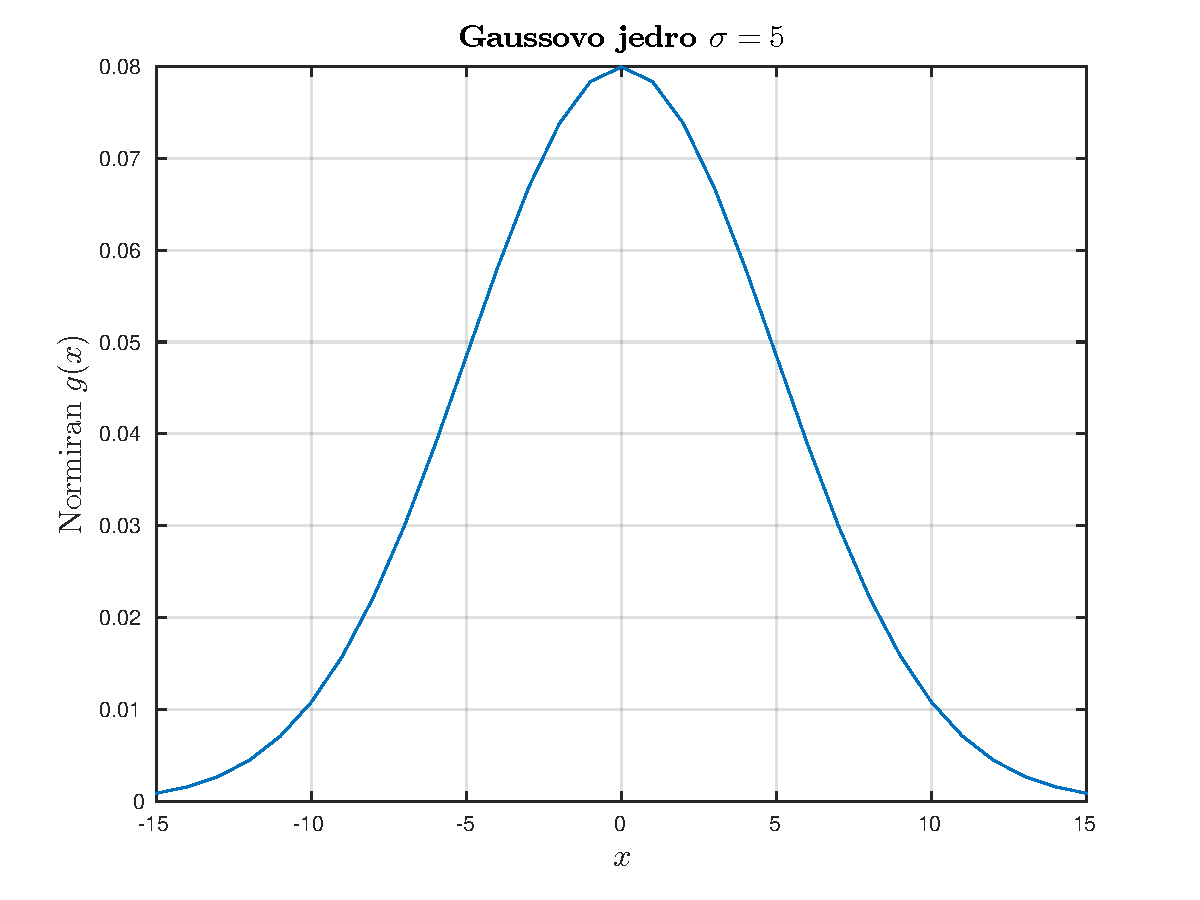
\includegraphics[width=0.7\columnwidth]{gauss-kernel-sl}
\caption[Gaussovo jedro s standardnim odklonom $\sigma=5$]{Gaussovo jedro s standardnim odklonom $\sigma=5$. }
\label{fig:gauss}
\end{figure}


Gaussov filter je vrsta filtra tekočega povprečja, ki je zelo primeren za izločevanje odvečnega šuma \cite{smith1997scientist}. Ker je karakteriziran z impulznim odzivom, ki je simetričen okoli ničelnega vzorca, gre za vrsto filtra z ničelno fazo. To pomeni, da je faza v frekvenčnem prostoru vedno $0$ \cite{smith1997scientist}. Ker imamo pri takih filtrih negativne indekse, ga težje uporabljamo. 

Ponavadi filtre uporabljamo v rekurzivni obliki, saj je računanje hitrejše. Impulzni odziv rekurzivnega filtra ni simetričen, zato ima nelinearno fazo \cite{smith1997scientist}. To pomanjkljivost lahko odpravimo z uporabo dvosmernega filtriranja.

Pri \textbf{dvosmernem filtriranju} najprej filtriramo iz leve proti desni in nato iz desne proti levi \cite{smith1997scientist}. Dobljena signala združimo in dobimo pravilen rezultat.



\section{Evaluacijske metrike}
V predstavljenih enačbah je $N$ število vzorcev, $\hat{y}_i~ \forall i=1,\ldots,N$ so izmerjene vrednosti in $y_i ~\forall i=1,\ldots,N$ so prave vrednosti. Spremenljivke s prečno črto predstavljajo srednjo vrednost, ki jo izračunamo po enačbi~\eqref{eq:mean}~\cite{witten2005data}.

\begin{equation}
\overline{y} = \frac{1}{N} \sum_{i=1}^N y_i
\label{eq:mean}
\end{equation}


\subsection{Koren srednje kvadratične napake}
Koren srednje kvadratične napake (ang. Root Mean Square Error) (\rmse) opišemo z enačbo~\eqref{eq:rmse}~\cite{witten2005data}.
\begin{equation}
e_{RMS} = \sqrt{\frac{1}{N} \sum_{i=1}^{N}\left( \hat{y}_i - y_i \right)^2}
\label{eq:rmse}
\end{equation}

Rezultati se gibljejo na intervalu $e_{RMS} \in [0, \infty)$. Manjša vrednost pomeni boljši rezultat~\cite{witten2005data}.

\subsection{Koren relativne kvadratične napake}
Koren relativne kvadratične napake (ang. Relative Root Squared Error) (\rrse) opišemo z enačbo~\eqref{eq:rmse}~\cite{witten2005data}. $\overline{y}$ je srednja vrednost pravih vrednosti, ki jo izračunamo po enačbi~\eqref{eq:mean}.

\begin{equation}
e_{RRS} = \sqrt{\frac{\sum_{i=1}^{N} \left ( \hat{y}_i - y_i \right )^2}{\sum_{i=0}^{N} \left( \overline{y} - y_i \right)^2}}
\label{eq:rrse}
\end{equation}

Rezultati se gibljejo na intervalu $e_{RRS} \in [0, \infty)$. Manjša vrednost pomeni boljši rezultat~\cite{witten2005data}.

Enačbo si lahko razlagamo kot \rmse matematičnega modela, ki je normaliziran na \rmse najenostavnejšega matematičnega modela ali prediktorja~\cite{witten2005data}. Najenostavnejši prediktor je tisti, ki nam na izhodu daje srednjo vrednost $\overline{y}$. 

\subsection{Relativna absolutna napaka}
Relativno absolutno napako (ang. Relative Absolute Error) (\rae) opišemo z enačbo~\eqref{eq:rmse}~\cite{trucco1998introductory}.

\begin{equation}
e_{RA} = \frac{\sum_{i=1}^{N} \left | \hat{y}_i - y_i \right |}{\sum_{i=1}^{N} \left| \overline{y} - y_i \right|}
\label{eq:rae}
\end{equation}

Rezultati se gibljejo na intervalu $e_{RAE} \in [0, \infty)$. Manjša vrednost pomeni boljši rezultat~\cite{witten2005data}.

\subsection{Korelacijski koeficient}
Korelacijski koeficient \corr je predstavljen z enačbo~\eqref{eq:r}~\cite{witten2005data}.

\begin{subequations}
\begin{align}
\corr &= \frac{S_{\hat{y}y}}{\sqrt{S_{\hat{y}} S_y}} \\
S_{\hat{y}y} &= \frac{\sum_{i=1}^N \left(\hat{y}_i - \overline{\hat{y}}\right)\left(y_i - \overline{y}\right) }{N-1} \\
S_{\hat{y}} &= \frac{\sum_{i=1}^N \left(\hat{y}_i - \overline{\hat{y}}\right)}{N-1} \\
S_y &= \frac{\sum_{i=1}^N \left(y_i - \overline{y}\right) }{N-1}
\end{align}
\label{eq:r}
\end{subequations}

Rezultati se gibljejo na intervalu $e_{RAE} \in [-1, 1]$~\cite{witten2005data}. Vrednost $-1$ pomeni da so rezultati popolnoma korelirani s pravimi vrednostmi v nasprotni smeri. Vrednost $0$ pomeni, da ne obstaja nobena korelacija. Vrednost $1$ pomeni, da obstaja popolna korelacija.  


\subsection{Razmerje signal in šum}
Razmerje signal šum (ang. Signal to Noise Ratio) (SNR) je določeno z enačbo~\eqref{eq:snr}, kjer je $P_s$ moč signala $y$ in $P_n$ moč šuma $n$~\cite{gonzalez2006digital}. Signal z nizko vsebnostjo šuma ima visok SNR, medtem, ko nizek SNR pomeni veliko šuma v signalu.

\begin{subequations}
\begin{align}
SNR_{dB} &= 10 \log_{10}\left(\frac{P_s}{P_n}\right) \\
P_s &= \frac{1}{N} \sum_{i=1}^{N} y_i^2 \\
P_n &= \frac{1}{N} \sum_{i=1}^{N} n_i^2
\end{align}
\label{eq:snr}
\end{subequations}



\subsection{Mera prekrivanja področja}
Mera prekrivanja področja (ang. Region Overlap), ki je predstavljena z enačbo~\ref{eq:region-overlap} se večinoma uporablja za sledilnike~\cite{vcehovin2016visual}. $\Lambda$ predstavlja opis tarče, $R_t$ je področje tarče ob času $t$, $N$ je število slik v zaporedju, $G$ predstavlja referenco in $T$ tarčo.

\begin{subequations}
\begin{align}
	\Lambda &= \left\{R_t\right\}^N_{t=1}, \nonumber \\
	\Phi(\Lambda^G, \Lambda^T) &= \left\{\phi_t\right\}^N_{t=1}, \nonumber \\
    \phi_t &= \frac{R_t^G \cap R_t^T }{R_t^G \cup R_t^T} 
\end{align}
\label{eq:region-overlap}
\end{subequations}


S prekrivanjem področja dobimo rezultate na intervalu $\left[0,1\right]$. Večje število predstavlja boljši rezultat.




\chapter{Eksperimenti}\label{sec:eksperimenti}
V tem poglavju predstavljamo eksperimente, ki smo jih izvedli v dveh različnih okoljih: v fiziološkem laboratoriju in na squash igrišču (terenski testi). Z njimi smo naslovili energijsko porabo $eem(t)$, kot osrednji fiziološki parameter. Srčni utrip $hr(t)$ smo obravnavali kot sekundarni parameter, z razumevanjem, da slabo odraža dejansko energijsko porabo. Z eksperimenti detekcije dihanja smo želeli preizkusiti predlagano metodo za širšo uporabo.

Pri vseh naslovljenih fizioloških parametrih smo s pomočjo strojnega učenja izvajali predikcijo časovnih signalov $eem(t)$ za energijsko porabo, $hr(t)$ za srčni utrip in $dihanje(t)$ za dihanje. Predikcijo smo izvajali iz posamezne slike zaporedja video posnetka. Pri tem smo najprej generirali sliko optičnega ali prostorskega toka in nato določili področje, kjer se nahaja merjenec. Iz izbranega področja smo izračunali vektorje značilk $\vec{x}(t)$, te pa smo uporabili za predikcijo. Rezultat je zelo enostaven, skoraj realno-časoven model, ki ga lahko razširimo s temporalnim modeliranjem, če bi se pojavila potreba. 

Prvi del postopka je učenje SVM/SVR modela, kot je prikazano na sliki~\ref{fig:shema-generalnega-postopka01}. Na ta način dobimo parametre regresijskega modela, ki jih nato uporabimo za napovedovanje porabe energije iz testnih podatkov, kot je prikazano na sliki~\ref{fig:shema-generalnega-postopka02}.

\begin{figure}[!htb]
	\centering
	\resizebox{\columnwidth}{!}{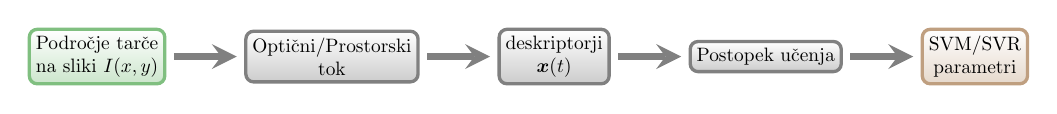
\begin{tikzpicture}
% LAYERS
\pgfdeclarelayer{bg}
\pgfsetlayers{bg,main}
\tikzset{
	between/.style args={#1 and #2}{
		at = ($(#1)!0.5!(#2)$)
	}
}

% NODES
\node (slika) [input] at (0,0) {Področje tarče\\na sliki $I(x,y)$};

\node (of) [block, right= of slika] {Optični/Prostorski\\tok};
\node (hoof) [block, right= of of] {deskriptorji\\$\vec{x}(t)$};


\node (ucenje) [block, right=of hoof] {Postopek učenja};

\node (rezultat) [output, right= of ucenje] {SVM/SVR\\parametri};

% arrows
\draw [arrow] (slika) -- (of);


\draw [arrow] (of) -- (hoof);
\draw [arrow] (hoof) -- (ucenje);

\draw [arrow] (ucenje) -- (rezultat);
\end{tikzpicture}}
	\caption[Shema generalnega postopka učenja]{Shema generalnega postopka učenja. Iz izbranega področja tarče generiramo sliko toka in izračunamo vekorje značilk $\vec{x}(t)$. Te nato uporabimo za učenje realno-časovnih modelov, s katerimi izvajamo predikcijo nad fiziološkimi parametri.}
	\label{fig:shema-generalnega-postopka01}
\end{figure}

\begin{figure}[!htb]
	\centering
	\resizebox{\columnwidth}{!}{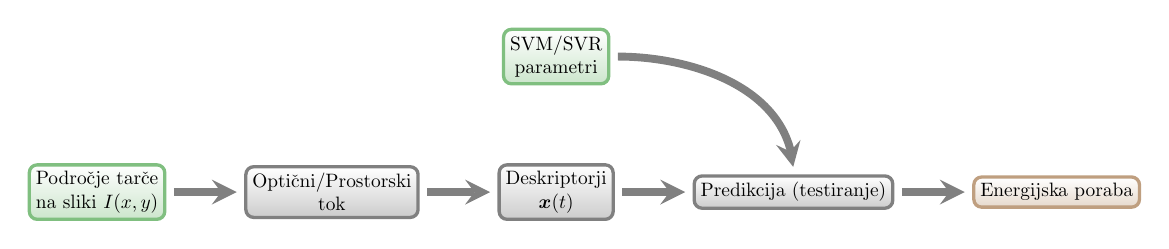
\begin{tikzpicture}
% LAYERS
\pgfdeclarelayer{bg}
\pgfsetlayers{bg,main}
\tikzset{
	between/.style args={#1 and #2}{
		at = ($(#1)!0.5!(#2)$)
	}
}

% NODES
\node (slika) [input] at (0,0) {Področje tarče\\na sliki $I(x,y)$};

\node (of) [block, right= of slika] {Optični/Prostorski\\tok};
\node (hoof) [block, right= of of] {Deskriptorji\\$\vec{x}(t)$};

\node (params) [input, above=of hoof] {SVM/SVR\\parametri};
\node (ucenje) [block, right=of hoof] {Predikcija (testiranje)};

\node (rezultat) [output, right= of ucenje] {Energijska poraba};

% arrows
\draw [arrow] (slika) -- (of);


\draw [arrow] (of) -- (hoof);
\draw [arrow] (hoof) -- (ucenje);
\draw [arrow,] (params) to[out=0,in=90] (ucenje);

\draw [arrow] (ucenje) -- (rezultat);
\end{tikzpicture}}
	\caption[Shema generalnega postopka predikcije]{Shema generalnega postopka predikcije. Vhodni podatki so testni podatki.}
	\label{fig:shema-generalnega-postopka02}
\end{figure}

Eksperimente smo kronološko razdelili na dve fazi. V \emph{1. fazi} smo analizirali observabilnost izbranih fizioloških parametrov. Parameter je observabilen, če obstaja neničelna (pozitivna) korelacija med našo estimacijo iz značilk gibanja in merjenih vrednosti, ki smo jih dobili iz zanesljivih metod pridobivanja fizioloških parametrov. %V 1. fazi smo posebej naslovili preliminarne teste, laboratorijske eksperimente tekalne steze, terenske eksperimente squash igre ter eksperimente dihanja. V {preliminarnih testih} opisujemo teste, s katerimi smo določili optimalne vrednosti parametrov. 
V \emph{eksperimentih 2. faze} smo optimizirali segmente postopka estimacije fizioloških parametrov. %Sledi končna preiskava. Končna preiskava je sestavljena iz preliminarnih testov, laboratorijske in terenske preiskave. V preliminarnih testih smo optimizirali dele postopka, s katerim smo v 1. fazi eksperimentov dobili najboljše rezultate. V laboratorijskih in terenskih preiskavah smo uporabili tri različne protokole.

\renewcommand{\folder}{./pogl/03-eksperimenti}
\section{Eksperimenti 1. faze}
\subsection{Preliminarni testi}
\subsubsection{Optimizacija HOOF deskriptorjev}\label{sec:optimizacija-hoof}
Parameter $N_{HOOF}$ smo določili na podlagi rezultatov iz poglavja \ref{sec:rezultati-optimizacija-hoof}. Za evaluacijo smo uporabili učne vzorce hrbtne kamere preliminarnih laboratorijskih testov. Evaluirali smo samo za podatke energijske porabe $W$. Pridobljene značilke deskriptorjev smo normirali na intervalu $[-1,1]$ in jih uporabili za učenje regresijskega modela z metodo podpornih vektorjev $\epsilon$-SVR in jedrom RBF. Metode so podrobneje predstavljene v poglavju \ref{sec:matematicni-modeli}. Za določitev optimalnih parametrov, ki so predstavljeni v tabeli \ref{tab:nhoof-param}, smo uporabili optimizacijsko metodo mrežnega iskanja \cite{hsu2003practical}. Rezultate smo filtrirali še s Kalmanovim filtrom, ki je predstavljen v \ref{sec:kalmanov-filter}.

\begin{table}[htb]
	\centering
	\begin{tabular}{S[table-format=2.0] S[table-format=2.3] S[table-format=1.3] S[table-format=1.3] S[table-format=1.3]}
		\toprule
		\thead{$\mathbf{N_{HOOF}}$} & \thead{$\mathbf{C}$} & \thead{$\mathbf{\gamma}$} & \thead{$\mathbf{\epsilon}$} & \thead{MSE} \\ 
		\midrule
		30 & 8 & 0.707 & 0.812 & 7.903 \\
		60 & 8 & 0.354 & 0.379 & 7.320 \\
		120 & 11.314 & 0.177 & 0.536 & 6.998 \\
		160 & 11.314 & 0.125 & 0.616 & 6.832 \\
		\bottomrule
	\end{tabular}
	\caption[Optimalni parameteri RBF jedra modelov za določitev $N_{HOOF}$]{Optimalni parametri RBF jedra za modele z različnim številom stolpcev $N_{HOOF}$ v HOOF deskriptorju. Z njimi smo učili modele s katerimi smo preverjali optimalno število stolpcev v HOOF deskriptorju}
	\label{tab:nhoof-param}
\end{table}







\subsubsection{Optimizacija HAFA deskriptorjev}
Parameter $N_{HAFA}$ smo določili na podlagi rezultatov \ref{sec:rezultati-optimizacija-hafa}. Za evaluacijo smo uporabili enak eksperimentalni protokol kot za HOOF značilke v poglavju \ref{sec:hoof}, s to razliko, da smo značilke normirali na intervalu $[0, 1]$ in odstranili stolpec z amplitudami $0.5$. S tem smo odstranili šum, ki se je pojavil, ko ni bilo nobenega gibanja. Amplitudo šuma smo določili, kot maksimalno vrednost amplitude, ki še ni predstavljala gibanja. Optimalni parametri evaluacijske metode so predstavljeni v tabeli \ref{tab:nhafa-param}.


\begin{table}[!htb]
	\centering
	\begin{tabular}{S[table-format=2.0] S[table-format=2.3] S[table-format=1.3]  S[table-format=1.3] S[table-format=1.3]}
		\toprule
		\thead{$\mathbf{N_{HAFA}}$} & \thead{$\mathbf{C}$} & \thead{$\mathbf{\gamma}$} & \thead{$\mathbf{\epsilon}$} & \thead{MSE} \\ 
		\midrule
		30 & 8 & 5.657 & 0.616 & 4.329 \\
		60 & 8 & 5.657 & 0.616 & 4.327 \\
		120 & 8 & 5.657 & 0.616 & 4.327 \\
		160 & 8 & 5.657 & 0.616 & 4.327 \\
		\bottomrule
	\end{tabular}
	\caption[Optimalni parameteri RBF jedra modelov za določitev $N_{HAFA}$]{Optimalni parametri RBF jedra za modele z različnim številom stolpcev $N_{HAFA}$ v HAFA deskriptorju. Z njimi smo učili modele s katerimi smo preverjali optimalno število stolpcev v HAFA deskriptorju.}
	\label{tab:nhafa-param}
\end{table}






\subsubsection{Razširitev HOOF deskriptorja}\label{sec:razsiritev-hoof-rezultati}
HOOF deskriptorju smo pripeli HAFA deskriptor in tako dobili razširjeni deskriptor HOOF-HAFA, ki po evaluaciji iz poglavja \ref{sec:rezultati-razsiritev-hoof} v splošnem daje boljše rezultate.

Pri evaluaciji deskriptorjev HOOF in HOOF-HAFA smo uporabili učne vzorce hrbtne kamere terenskih testov. Evaluirali smo za podatke srčnega utripa $hr$. Srčni utrip smo za gradnjo modelov pretvorili v energijsko porabo $W$ po enačbi \eqref{eq:charlot}. Pridobljene značilke smo normirali na intervalu [0,1] in jih uporabili za učenje regresijskega modela z metodo podpornih vektorjev $\epsilon$-SVR in jedrom RBF. Za določitev optimalnih parametrov, ki so predstavljeni v tabeli \ref{tab:nhoof-param}, smo uporabili optimizacijsko metodo mrežnega iskanja \cite{hsu2003practical}. Rezultate smo filtrirali še s Gaussovim jedrom (predstavljen v \ref{sec:gaussov-filter}) velikosti $6$ in varianco $\sigma=16$. 

\begin{table}[htb]
	\centering
	\begin{tabular}{l S[table-format=2.3] S[table-format=1.3] S[table-format=1.3] S[table-format=1.3]}
		\toprule
		\textbf{Deskriptor} & \thead{$\mathbf{C}$} & \thead{$\mathbf{\gamma}$} & \thead{$\mathbf{\epsilon}$} & \thead{MSE} \\ 
		\midrule
		HOOF & 2.828 & 11.314 & 0.435 & 2.192 \\
		HOOF-HAFA & 5.657 & 2.828 & 0.154 & 1.781 \\
		\bottomrule
	\end{tabular}
	\caption[Optimalni parameteri RBF jedra modelov za izbiro deskriptorjev]{Optimalni parametri RBF jedra za modele z različnim deskriptorjem. Z modeloma smo preverjali razširitev HOOF deskriptorja v HOOF-HAFA deskriptor.}
	\label{tab:izbira-param}
\end{table}














\subsubsection{Testiranje sledilnikov za optični tok}\label{sec:testiranje-sledilnikov-za-opticni-tok}
Sledilnike smo testirali na sekvencah slik \textit{handball1} in \textit{handball2} podatkovne baze VOT2016 \cite{kristan2016visual}.Primer posnetkov je viden na sliki \ref{fig:testiranje-tracker-visual}. Sledila je še hitra vizualna ocena delovanja na kratkih izsekih video posnetka \cite{squashtv2014squash}. Primer posnetka je viden na sliki \ref{fig:testiranje-squash-1-kcf}.

\begin{figure}[!htbp]
	\centering
	
	\begin{subfigure}[t]{0.45\columnwidth}
		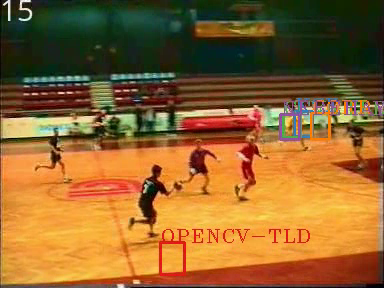
\includegraphics[width=\columnwidth]{handball1-example.png}
		\caption{15. slika posnetka \textit{handball1}.}
		\label{fig:testiranje-handball1}
	\end{subfigure}
	~
	\begin{subfigure}[t]{0.45\columnwidth}
		\includegraphics[width=\columnwidth]{handball2-example.png}
		\caption{111. slika posnetka \textit{handball2}.}
		\label{fig:testiranje-handball2}
	\end{subfigure}  
	\caption[Primer delovanja sledilnikov za \textit{handball} posnetke]{Primer delovanja sledilnikov za \textit{handball} posnetke. Referenčni igralec, ki mu morajo slediti ima rumeno majico. }
	\label{fig:testiranje-tracker-visual}
\end{figure}



\begin{figure}[htbp]
	\centering
	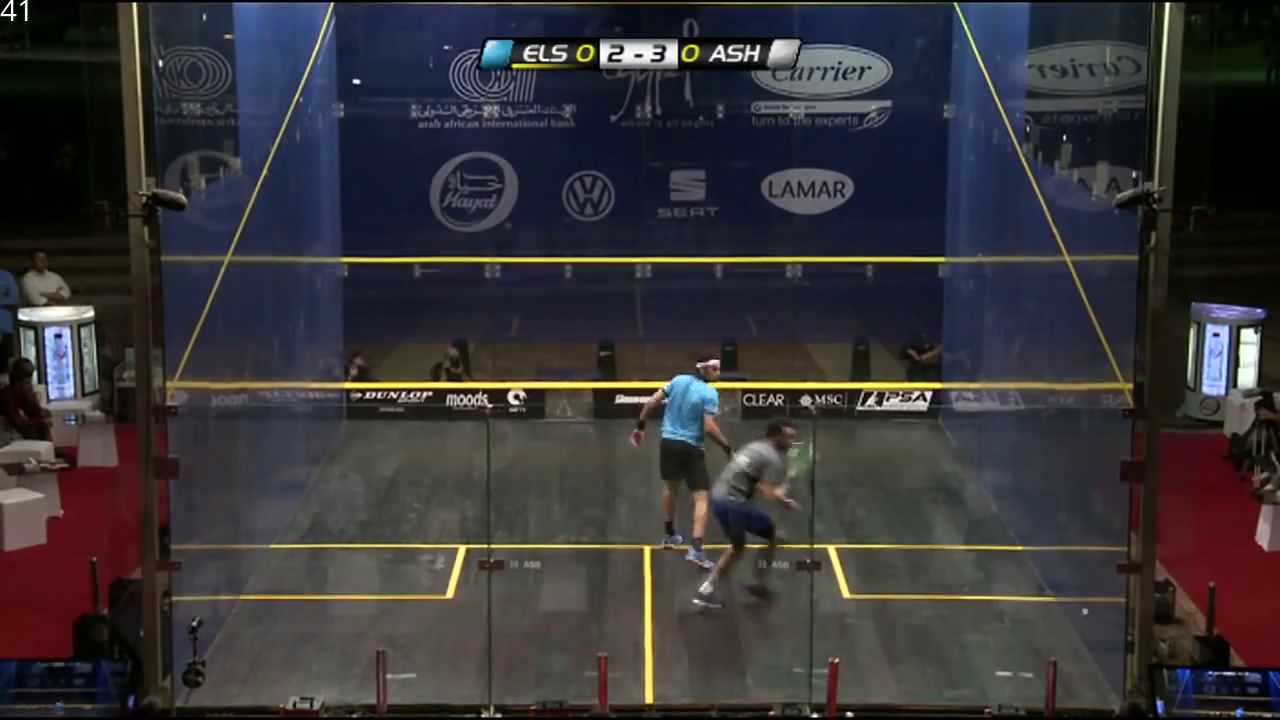
\includegraphics[width=0.6\columnwidth]{preliminary-squash-no-tracker.png}
	\caption[Uporaba squash posnetka za vizualno oceno delovanja sledilnikov]{Uporaba squash posnetka za vizualno oceno delovanja sledilnikov. Predstavljena je 41. slika posnetka \cite{squashtv2014squash}, kjer smo preizkušali KCF sledilnik. Sledili smo igralcu v svetlo modri majici. Modri okvir prikazuje področje, ki ga je sledilnik zaznal.}
	\label{fig:testiranje-squash-1-kcf}
\end{figure}



Pri testiranju sekvenc slik podatkovne baze VOT2016 smo poenostavili rotirajoča referenčna področja detekcij na nerotirajoča področja. Pri tem smo za zgornji levi kot $T_0(x,y)$ in spodnji desni kot $T_1(x,y)$ uporabili enačbo \eqref{eq:vot-bb}, kjer so $\left( x_i, y_i\right), \forall i=1,\ldots,4$ ogljišča rotirajočega referenčnega področja. 

\begin{equation}
\begin{aligned}
T_0(x,y) &= \left( \min_{i = 1,\ldots,4}\left\{x_i \right\}, 
\min_{i=1,\ldots,4}\{y_i \} \right) \\
T_1(x,y) &= \left( \max_{i = 1,\ldots,4}\left\{x_i \right\}, 
\max_{i=1,\ldots,4}\{y_i \} \right)
\end{aligned}
\label{eq:vot-bb}
\end{equation}

Ker je za naš sledilnik najbolj pomembno zanesljivo delovanje, smo izbrali mero prekrivanja področja.


Video posnetek \cite{squashtv2014squash} smo za potrebe vizualne ocene delovanja na squash posnetkih razdelili na več kratkih izsekov. Pri tem smo uporabili le hrbtne posnetke mirujoče kamere. 







\subsection{Laboratorijski eksperimenti tekalne steze}
Prve eksperimente smo izvedli v laboratoriju za fiziologijo na Fakulteti za šport. Merjenec je tekel na tekalni stezi ob prisotnosti operaterja---zdravnika, ki je določal intenziteto in čas trajanja obremenitve. Pri tem smo merili srčni utrip in enrgijsko porabo športnika (starost: 26 let, višina: \SI{177}{\cm}, teža: \SI{79.1}{\kg}, $VO_2max$: \SI{3705}{\ml\per\min}). Energijsko porabo smo merili z indirektno kalorimetrijo, in sicer s ``breath by breath'' Cosmed CPET Metabolic Cart \cite{beaver1973line}. Pri tem smo uporabili Hans Rudolph obrazno masko s predpisanim minimalnim VD (mrtvim prostorom).


\subsubsection{Pridobivanje podatkov}
Tekalno stezo smo snemali iz dveh različnih zornih kotov: hrbtni del in stranski del. Zaradi časovne neusklajenosti posnetkov smo jih sinhronizirali glede na začetno sliko meritev. Zaradi rahlo različne časovne frekvence na posameznih kamerah, se časovne neusklajenosti do potankosti nismo mogli znebiti. Ta se je akumulirala skozi čas. Pridobili smo posnetke barvnih RGB slik in infrardeče IR posnetke hrbtnega dela. Primer hrbtnega stranskega  in IR posnetka je prikazan na sliki \ref{fig:primer-posnetka-rgb-ir}.

\begin{figure}[htb]
	\centering
	\begin{subfigure}[t]{0.3\columnwidth}
		\centering
		\includegraphics[width=\columnwidth]{normal-sv-150.png}
		\caption{Stranska RBG slika.}
	\end{subfigure}
	~
	\begin{subfigure}[t]{0.3\columnwidth}
		\centering
		\includegraphics[width=\columnwidth]{normal-bv-150.png}
		\caption{Hrbtna RGB slika.}
	\end{subfigure}
	~
    \begin{subfigure}[t]{0.3\columnwidth}
    	\centering
		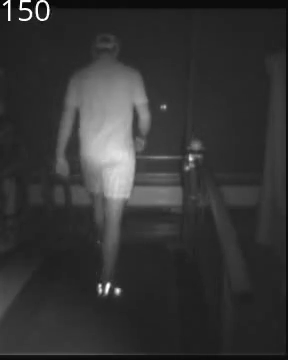
\includegraphics[width=0.6\columnwidth]{normal-ir-150.png}
		\caption{Hrbtna IR slika.}
	\end{subfigure}
	\caption[Hrbtna, stranska in IR 150. slika posnetkov iz prve serije]{Hrbtna, stranska in IR 150. slika posnetkov iz prve serije. Kljub časovni sinhronizaciji med posnetkoma, se časovni neusklajenosti nismo mogli popolnoma izogniti. Časovni frekvenci kamer nista bili sinhronizirani.}
	\label{fig:primer-posnetka-rgb-ir}
\end{figure}

Snemali smo v ločljivosti $480 \times 640$. Hitrost RGB posnetkov je bila \SI{30}{fps}, za IR posnetke pa je hitrost znašala \SI{25}{fps}.  Naklon tekalne steze je bil od \SI{1.5}{\%} do \SI{2}{\%}.



\subsubsection{Protokoli izvajanja meritev}
Naredili smo dve seriji testov v razmiku 20 minut. Fiziološke parametre smo vzorčili vsakih \SI{5}{\s}. V prvi seriji smo naredili 8 testov, kjer so vsi trajali 2 minuti. Hitrost tekalne steze smo vsak test povečali za \SI{1}{\km\per\hour}. Prvi test je imel hitrost  \SI{6}{\km\per\hour} zadnji pa \SI{13}{\km\per\hour}.

V drugi seriji smo naredili 3 teste po 5 minut. Hitrosti tekalne steze so bile  \SI{7}{\km\per\hour}, \SI{10}{\km\per\hour} in \SI{13}{\km\per\hour}.

Prvo serijo testov smo uporabili za pridobitev učnih vzorcev. Drugo serijo smo uporabili za testne vzorce.


\subsubsection{Elementarni postopek procesiranja}\label{sec:elementarni-postopek}
Kot smo že omenili so bile meritve fizioloških parametrov izvedene z vzorčenjem \SI{5}{\s} oziroma s frekvenco \SI{0.2}{\hertz}. Hitrost posnetkov je bila \SI{30}{fps} za RGB in \SI{25}{fps} za IR slike. Zaradi neskladja frekvenc vzorčenja slik in fizioloških parametrov, smo te interpolirali s pomočjo Matlabove funkcije \texttt{interp1}.
 
Za izbrano področje slike iz zaporedja posameznega posnetka smo nato izračunali optični tok. Primer dobljenega optičnega toka je prikazan na sliki \ref{fig:opticni-tok-stage1} Enote optičnega toka so \si{ppf}. Pomenijo število slikovnih elementov na sliko (ang. Pixel per Frame).


\begin{figure}[!htb]
	\centering
	\begin{subfigure}{0.45\columnwidth}
		\includegraphics[width=\columnwidth]{./Slike/normal-sv-150.png}
		\caption{Originalna slika.}
	\end{subfigure}
	~
	\begin{subfigure}{0.45\columnwidth}
	    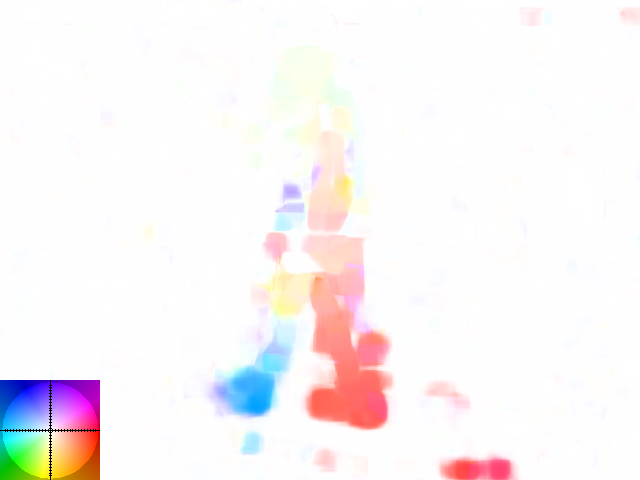
\includegraphics[width=\columnwidth, frame]{./Slike/normal-sv-of-coded-150.png}
		\caption{Slika optičnega toka.}
		\label{fig:stage1-of}
	\end{subfigure}
    \caption[Originalna $150$. stranska slika in optični tok]{Originalna $150$. stranska slika in njen optični tok. Gre za sliko 1. serije testov. Na sliki \subref{fig:stage1-of} je legenda barvnega kodiranja v spodnjem levem kotu s standardnim barvnim kodiranjem, ki je povzeto po \cite{baker2011database}. Maksimalna amplituda optičnega toka je na tej sliki znašala \SI{17}{ppf}.}
    \label{fig:opticni-tok-stage1}
\end{figure}

Sledilo je generiranje HOOF deskriptorjev, ki smo jih pred tem optimizirali po postopku, opisanem v poglavju \ref{sec:optimizacija-hoof}. Za parameter smo izbrali $N_{HOOF} = 60 $, ker je dal najbolj optimalne rezultate. Primer HOOF deskriptorjev lahko vidimo na sliki \ref{fig:hoof-znacilke}.

\begin{figure}[!htb]
	\centering
	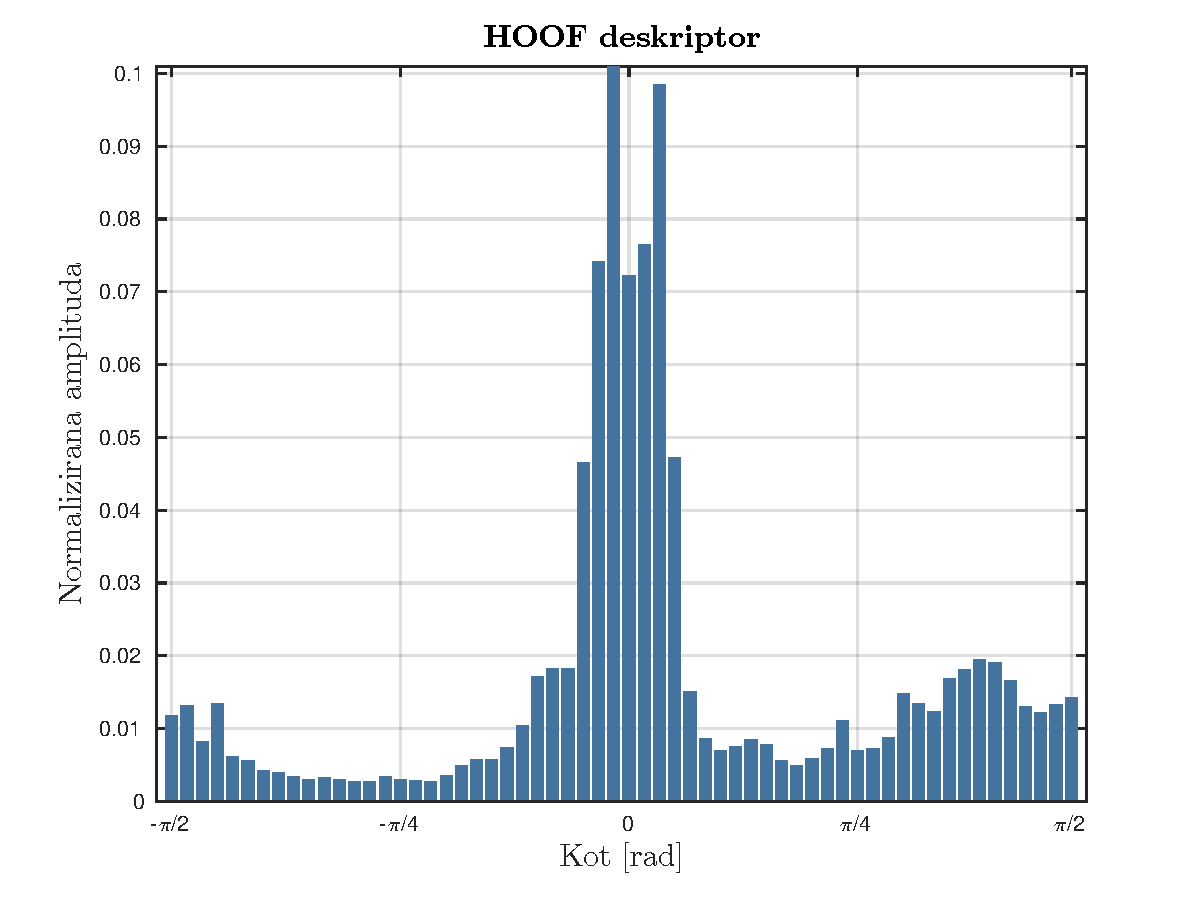
\includegraphics[width=0.75\columnwidth]{stage1-lab-sv-hist-sl}
	\caption[HOOF deskriptor za 150. RGB sliko prve serije]{HOOF deskriptor za 150. RGB sliko prve serije. Deskriptor smo izračunali iz slike \ref{fig:opticni-tok-stage1}.}
	\label{fig:hoof-znacilke}
\end{figure}

Modele smo učili z metodo podpornih vektorjev $\epsilon$-SVR in jedrom RBF. Regresijske parametre jedra smo optimizirali z metodo mrežnega iskanja. Naučili smo \num{8} elementarnih modelov, ki smo jih razdelili na dve kategoriji: na \textit{hr} modele, ki predvidevajo srčni utrip in modele \textit{eem}, ki predvidevajo porabo energije v \si{\kcal\per\min}. Kategoriji sta nadalje razdeljeni glede na zorni kot kamere: \textit{sv} modeli za stransko kamero in \textit{bv} modeli za hrbtno kamero. Eksperimente smo razširili z vpeljavo zakasnitve med referenčnim fiziološkim parametrom in merjenim parametrom iz slik posnetka. Z eksperimenti, ki so označeni z \textit{lag} kratico, smo preverili predlagano časovno zakasnitev med vzbujanjem in fiziološkim odzivom. 

Generirali smo tudi dodatne modele, in sicer: \textit{crop} modele, \textit{mixed} modele, \textit{track} modele, kjer smo uporabili sledilnik in obremenitvene modele. Ti so deljeni na \textit{scale} modele in \textit{proj} modele.

Vse tipe eksperimentov smo križno testirali glede na enak tip eksperimenta, le z drugim zornim kotom kamere. Uporabljen zorni kot kamere za križno testiranje je v imenih modelov zapisan v oklepajih. Rezultate smo pred testiranjem filtrirali s Kalmanovim filtrom. Uporabljeni parametri so opisani v poglavju \ref{sec:implementacija-kalman}.


\begin{figure}[!htb]
	\centering
	\resizebox{\columnwidth}{!}{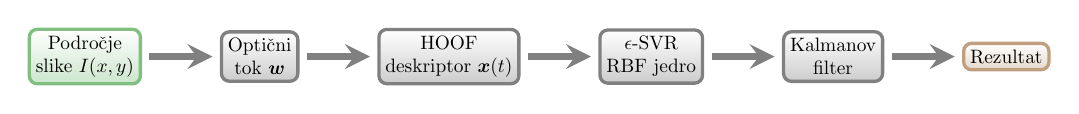
\begin{tikzpicture}
% LAYERS
\pgfdeclarelayer{bg}
\pgfsetlayers{bg,main}
\tikzset{
    between/.style args={#1 and #2}{
         at = ($(#1)!0.5!(#2)$)
    }
}

% NODES
\node (slika) [input] at (0,0) {Področje\\slike $I(x,y)$};

\node (of) [block, right= of slika] {Optični\\ tok $\vec{w}$};
\node (hoof) [block, right= of of] {HOOF\\deskriptor $\vec{x}(t)$};


\node (ucenje) [block, right=of hoof] {$\epsilon$-SVR\\RBF jedro};
\node (kalman) [block, right= of ucenje] {Kalmanov\\filter};


\node (rezultat) [output, right= of kalman] {Rezultat};

% arrows
\draw [arrow] (slika) -- (of);
\draw [arrow] (of) -- (hoof);
\draw [arrow] (hoof) -- (ucenje);
\draw [arrow] (ucenje) -- (kalman);
\draw [arrow] (kalman) -- (rezultat);
\end{tikzpicture}}
	\caption[Diagram postopka za eksperimente 1. faze]{Diagram postopka za eksperimente 1. faze. Izbranemu področju na sliki določimo optični tok.}
	\label{fig:diagram-procesiranja-stage1}
\end{figure}

\subsubsection{Določitev dodatne zakasnitve}
Na podlagi slike \ref{fig:lag-estimation-stage1} smo določili dodatno zakasnitev spremembe hitrosti tekalne steze. Z vpeljavo zakasnitve smo želeli preveriti pravilnost sinhronizacije merjenih podatkov in kamere. Celoten odziv posameznega fiziološkega parametra je prikazan na sliki \ref{fig:odziv-stage1}.


\begin{figure}[!htb]
	\centering
	\begin{subfigure}[t]{0.45\columnwidth}
		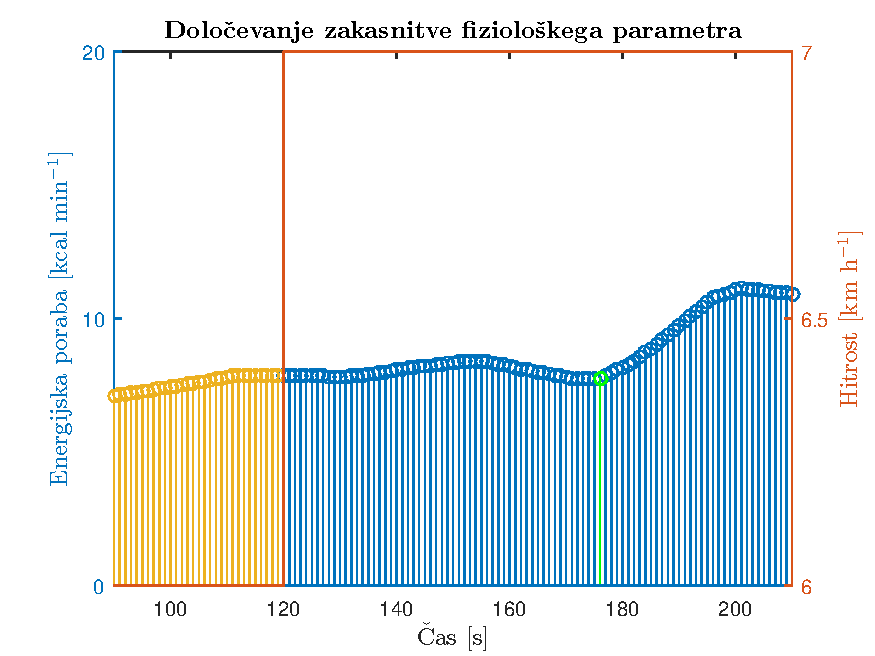
\includegraphics[width=\columnwidth]{stage1-lag-estimation-eem-sl}
		\caption{Zakasnitev za energijsko porabo.}
		\label{fig:lag-estimation-train-eem}
	\end{subfigure}
	~
	\begin{subfigure}[t]{0.45\columnwidth}
		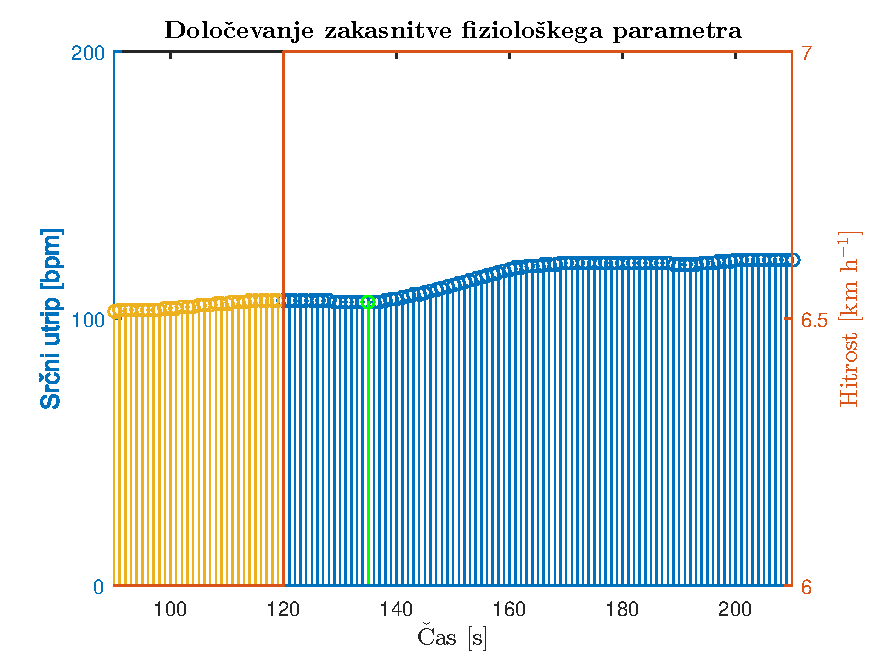
\includegraphics[width=\columnwidth]{stage1-lag-estimation-hr-sl}
		\caption{Zakasnitev za srčni utrip.}
		\label{fig:lag-estimation-train-hr}
	\end{subfigure}
	\caption[Prikaz določevanja dodatne zakasnitve]{Prikaz določevanja dodatne zakasnitve. Na posameznem grafu so prikazani vzorci fiziološkega parametra. Rumena barva označuje vzorce pred spremembo hitrosti tekalne steze, modra pa vzorce po spremembi. Sprememba hitrosti tekalne steze je prikazana z rdečo stopnico. Zeleno obarvani vzorec se nahaja ob trenutku, ko nastane fiziološki odziv.}
	\label{fig:lag-estimation-stage1}
\end{figure}

Zamik za srčni utrip je znašal \SI{15}{\s}. Za energijsko porabo smo izmerili \SI{55}{\s} zamika. Izbrane parametre smo testirali s zakasnitvenimi modeli s kratico \textit{lag}.

Zakasnitev smo določili, kot časovni interval od trenutka spremembe hitrosti tekalne steze do trenutka, ko se je vrednost fiziološkega parametra začela močneje povečevati. Pri tem smo izbrali spremembo hitrosti med prvim in drugim testom, saj je bil signal fiziološkega parametra na tem območju najbolj ustaljen. Kadar je povečevanju dokaj hitro sledil upad, smo smatrali, da do odziva še ni prišlo. Tak primer je prikazan na sliki \ref{fig:lag-estimation-stage1}\subref{fig:lag-estimation-train-eem}), kjer prvemu povečevanju za spremembo hitrosti tekalne steze sledi upad. 


\begin{figure}[!htb]
	\centering
	\begin{subfigure}[t]{0.45\columnwidth}
		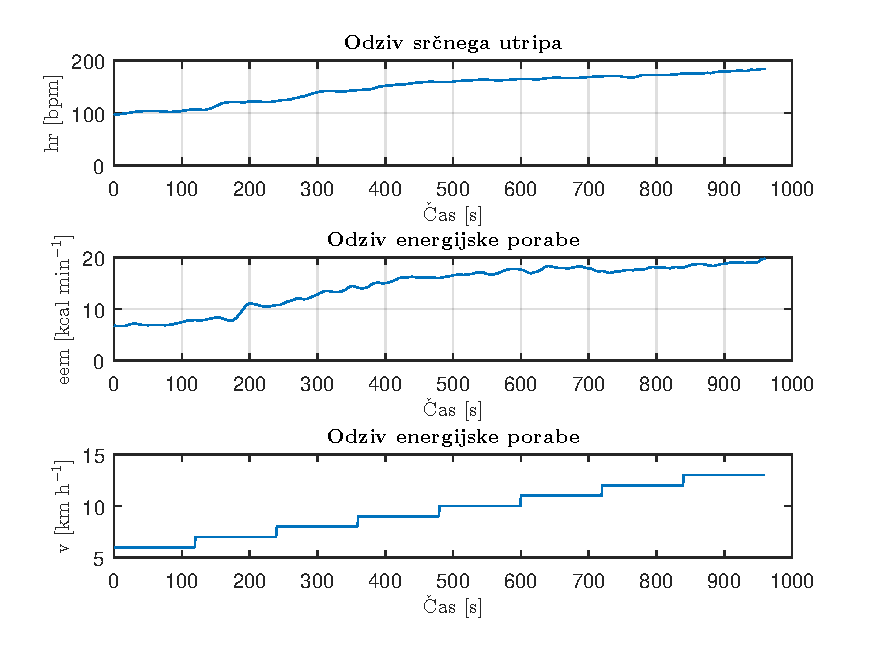
\includegraphics[width=\columnwidth]{odziv1-sl}
		\caption{Odziv učnih vzorcev.}
		\label{fig:odziv-ucnih-stage1}
	\end{subfigure}
	~
	\begin{subfigure}[t]{0.45\columnwidth}
		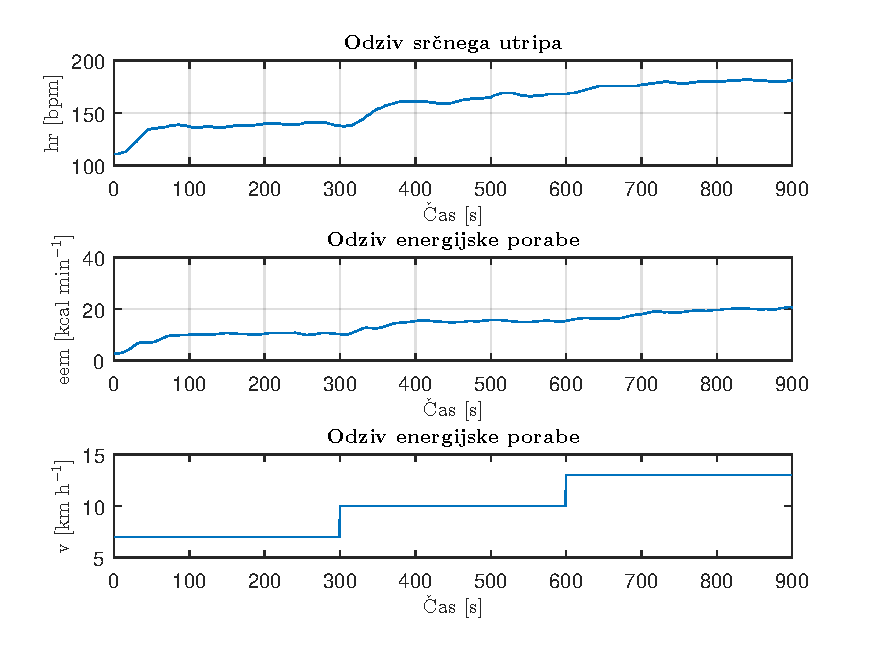
\includegraphics[width=\columnwidth]{odziv2-sl}
		\caption{Odziv testnih vzorcev.}
		\label{fig:odziv-testnih-stage1}
	\end{subfigure}
	\caption[Odziv posameznih fizioloških parametrov za obe seriji testov]{Odziv posameznih fizioloških parametrov za obe seriji testov.}
	\label{fig:odziv-stage1}
\end{figure} 


\subsubsection{Ročna določitev področja tarče}
HOOF deskriptorji so v teoriji robustni na šum, saj ta zaradi majhnih amplitud nima vpliva na obliko histograma. Vseeno pa se lahko pojavijo anomalije, ki povečajo amplitudo šuma na raven vrednosti merjenca. Pri tem mislimo predvsem na objekte in osebe v ozadju, ki se premikajo. Temu se lahko preprosto izognemo z določevanjem področja tarče. Ker je bil prizor na posnetkih razmeroma enostaven in ciklično monoton, smo se za preizkus naše hipoteze odločili, da bomo področja najprej določili ročno. Področja smo izbrali tako, da je bil merjenec ves čas skozi posnetek v izbranem področju. Izbrana področja za posamezne posnetke so predstavljena v tabeli \ref{tab:rocna-podrocja}, pri čemer so $h$ dolžina slike $w$ širina slike ter $x$ in $y$ slikovni koordinati. Vsi nadaljnji testi razen, kjer se uporablja sledilnik, temeljijo na izrezanih posnetkih, glede na ta področja.

\begin{table}[!htb]
	\centering
	\begin{tabular}{l l l S[table-format=3] S[table-format=2] S[table-format=3] S[table-format=3]}
		\toprule
		\multicolumn{3}{c}{}& \multicolumn{4}{c}{\textbf{Področje}} \\
		\cmidrule{4-7}
		\textbf{Serija} & \textbf{Pogled} & \textbf{Vrsta} & \thead{$\mathbf{x}$} & \thead{$\mathbf{y}$} & \thead{$\mathbf{w}$} & \thead{$\mathbf{h}$}  \\
		\midrule
		\multirow{3}{*}{1} & \multirow{2}{*}{hrbtni} & RGB & 228 & 43 & 207 & 437 \\
		&& IR & 32 & 10 & 167 & 329 \\
		& stranski & RGB & 179 & 31 & 346 & 420 \\
		\midrule
		\multirow{3}{*}{2} & \multirow{2}{*}{hrbtni} & RGB & 230 & 51 & 228 & 429 \\
		&& IR & 29 & 11 & 181 & 338 \\
		& stranski & RGB & 182 & 33 & 351 & 423 \\
		\bottomrule
	\end{tabular}
	\caption[Ročno izbrana področja tarče za posamezne posnetke]{Ročno izbrana področja tarče za posamezne posnetke. $x$ in $y$ sta koordinati zgornjega levega kota področja. $w$ in $h$ sta širina in dolžina področja.}
	\label{tab:rocna-podrocja}
\end{table}

\subsubsection{Združevanje posnetkov}
V dodatnih \textit{mixed} modelih, smo združili posnetke kamer z različnim zornim kotom. Združeni posnetek je bil po vrstnem redu sestavljen in posnetka stranske kamere in posnetka hrbtne kamere. Pri tem smo uporabili izrezane posnetke glede na ročno določena področja. Z združenim posnetkom smo želeli preveriti vpliv povečevanja informacije o gibanju merjenca zaradi uporabe različnih zornih kotov. 

\subsubsection{Obremenitveni testi}
Z obremenitvenimi testi smo želeli preizkusiti robustnost našega postopka. Opravili smo dve vrsti testov, in sicer: \textit{scale} teste in \textit{proj} teste. Pri \textit{scale} testih smo posnetke zmanjšali za \SI{50}{\%}. S tem smo simulirali večjo oddaljenost merjenca od kamere in tako preverili teoretično invariantnost HOOF deskriptorjev glede na skalo.

Z vnašanjem projektivne transformacije v posnetke smo s \textit{proj} testi preizkušali robustnost celotnega postopka na deformacije slike, ki jo lahko vnašajo leče kamere. Projektivno transformacijo smo izvedli s pomočjo Matlabovih funkcij \texttt{fitgeotrans} in \texttt{imwarp}. Za vhodne točke smo izbrali robove posamezne slike zaporedja. Za izhodne točke smo izbrali vrednosti v tabeli \ref{tab:projective}, pri čemer so $h$ dolžina slike, $w$ širina slike ter $x$ in $y$ slikovni koordinati.

\begin{table}[!htb]
	\centering
	\begin{tabular}{l S[table-format=1.3] S[table-format=1.3] }
		\toprule
		\thead{Točka} & \thead{$\mathbf{x~[\times w]}$} & \thead{$\mathbf{y~[\times h]}$} \\
		\midrule
		$P_0$ & 0 & 0.25 \\
		$P_1$ & 1 & 0 \\
		$P_2$ & 0.125 & 0.75 \\
		$P_3$ & 0.875 & 0.875 \\
		\bottomrule
	\end{tabular}
	\caption[Tabela pozicij robov transformirane slike]{Tabela pozicij robov transformirane slike. $h$ je dolžina slike, $w$ širina slike ter $x$ in $y$ slikovni koordinati.}
	\label{tab:projective}
\end{table}


\begin{figure}[!htb]
	\centering
	\begin{subfigure}[t]{0.45\columnwidth}
		\centering
		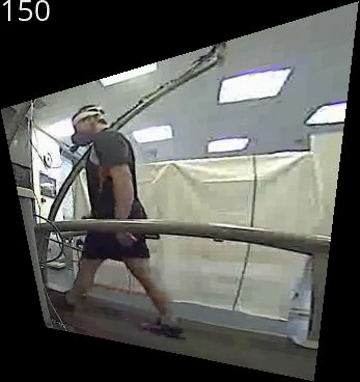
\includegraphics[width=0.6\columnwidth]{projective-sv-150.png}
		\caption{Stranska slika}
	\end{subfigure}
	~
	\begin{subfigure}[t]{0.45\columnwidth}
		\centering
		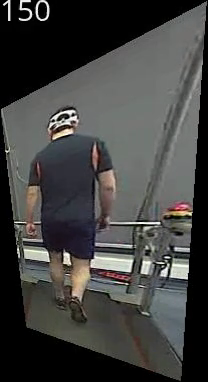
\includegraphics[width=0.4\columnwidth]{projective-bv-150.png}
		\caption{Hrbtna slika}
	\end{subfigure}
	\caption[Primer projektivne transformacije 150. slike posnetka iz prve serije]{Primer projektivne transformacije 150. slike posnetka iz prve serije. Prikazani sta stranska in hrbtna transformirana slika. Transformirali smo slike \ref{fig:primer-posnetka-rgb}.}
	\label{fig:projective}
\end{figure}


\subsubsection{Sledenje merjencem}\label{sec:tracking}
Obstaja veliko ekipnih športov, kjer sodeluje več igralcev. Ker so vsi vidni na vsaki sliki zaporedja posnetka, je nujno, da v naš sistem uvedemo funkcionalnost sledenja. S sledenjem na tekalni stezi smo preverili delovanje te funkcionalnosti. Rezultati, ki vsebujejo korak sledenja imajo kratico \textit{tr}. Primer sledenja je prikazan na sliki \ref{fig:sledenje}.

\begin{figure}[!htb]
	\centering
	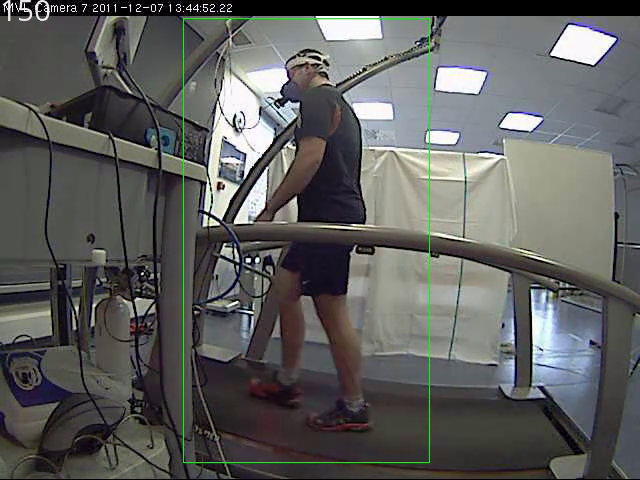
\includegraphics[width=0.6\columnwidth]{normal-sv-test-kcf2.png}
	\caption[Sledenje merjencu s KCF na stranski sliki]{Sledenje merjencu s KCF na stranski sliki. Prikazana je 150. slika RGB posnetka druge serije. Zeleni okvir prikazuje področje, ki ga je detektiral sledilnik.}
	\label{fig:sledenje}
\end{figure} 

Za sledenje smo uporabili KCF sledilnik, ki je implementiran v OpenCV knjižnici. Izbiro sledilnika smo opredelili že v poglavju \ref{sec:testiranje-sledilnikov-za-opticni-tok}. Pri sledenju smo uporabili sledeče parametre: pasovna širina Gaussovega jedra $0.2$, linearni interpolacijski faktor za adaptacijo $0.075$, regularizacijski faktor $0.01$, največja velikost obliža (ang. Patch) $6400$, prostorska pasovna širina $0.0625$, aktivirano skaliranje značilk za izboljšanje hitrosti procesiranja, razcepljeni učni koeficienti na dve matrike, dekativirano zavijanje (ang. wrapping) okoli vrednosti jedra, nekompresirani deskriptorji za sivinske slike in kompresirani za barvne slike, aktivirana PCA metoda za kompresijo značilk, velikost kompresije $2$ in  stopnja učenja kompresije $0.15$.

KCF sledilnik smo inicializirali z ročnim obkroževanjem področja tarče na prvi sliki vsakega posnetka. Področja tarče, ki jih je izbral sledilnik, smo uporabili za izrezovanje področij merjenca iz slik optičnega toka. HOOF deskriptorje smo izračunali le na izbranem področju. 



\subsubsection{Simulacija vibracij kamere}
Kadar uporabljamo ročne kamere, pogosto pride do tresenja. Vibracije smo simulirali z majhnimi naključnimi premiki in rotacijo posameznih slik iz video zaporedja. Vsako sliko smo transformirali z Evklidsko transformacijo. Pri tem smo translacijo omejili na \SI{4}{\%} velikosti slike. Rotacija je bila omejena na \SI{0.13}{rad}. 

Translacijo in rotacijo smo filtrirali še s Kalmanovim filtrom, tako da smo dobili bolj realistično simulacijo. Za Kalmanov filter smo uporabili enak model, kot je predstavljen v poglavju \ref{sec:kalmanov-filter}. Začetne variance filtra smo določili empirično tako, da smo dobili čimbolj realistične rezultate. Varianca šuma merilnega modela je znašala $\sigma_\vec{z}^2=1024$, varianca šuma modela gibanja pa $\sigma_\vec{x}^2=2$. Za kovariančno matriko predikcije smo uporabili varianco $\sigma_\vec{P}^2=2$.

S simulacijo vibracij smo naredili obremenitveni test za modele z vključenim sledilnikom. Rezultati so anotirani s \textit{sh} kratico. Primer delovanja sledilnika je prikazan na sliki \ref{fig:vibracije}.

\begin{figure}[!htb]
	\centering
	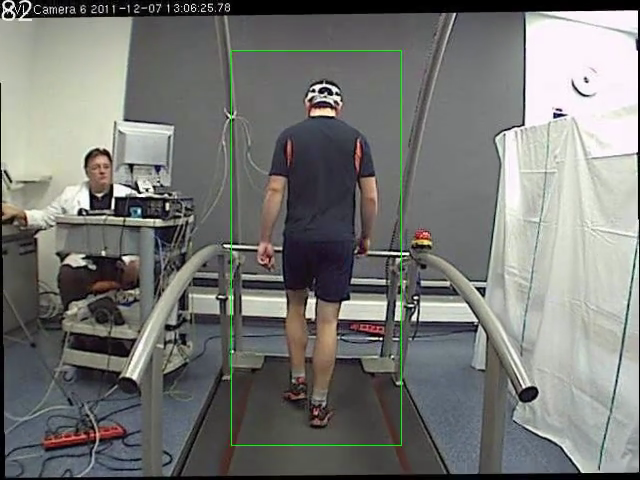
\includegraphics[width=0.6\columnwidth]{shake-bv-train-kcf2.png}
	\caption[Sledenje merjencu na tresočem posnetku]{Sledenje merjencu na tresočem posnetku. Prikazana je 82. slika hrbtnega RGB posnetka prve serije. Zeleni okvir prikazuje področje, ki ga je detektiral KCF sledilnik.}
	\label{fig:vibracije}
\end{figure} 








\subsection{Terenski eksperimenti squash igre}
Pri terenskih eksperimentih smo snemali dve squash igri z enim setom z RaspberryPi in RaspiCam napravo v resoluciji  $1920 \times 1080$. Zaradi nezadovoljivih podatkov druge igre, smo za učenje in testiranje modelov uporabili le prvo igro. Igralcem smo merili srčni utrip s kontaktnimi senzorji. 

Prvega igralca prve igre  (starost: 45 let, velikost: \SI{176}{\cm}, teža: \SI{68}{\kg}, spol: male, $hr_{tmax}$: \SI{179}{bpm}, $hr_{r}$: \SI{45}{bpm}) smo uporabili za učne vzorce. Drugega igralca (starost: 17 let, višina: \SI{178}{\cm}, teža: \SI{66}{\kg}, spol: male, $hr_{tmax}$: \SI{203}{bpm}, $hr_{r}$: \SI{50}{bpm}) smo uporabili za testne vzorce. 

\subsubsection{Razširitev HOOF deskriptorja}
Chaudhry et al. \cite{chaudhry2009histograms} predlaga uporabo histogramov orientiranega optičnega toka (HOOF) za estimacijo gibanja. Vendar pa smo v terenskih testiranjih ugotovili, da njihova uporaba v realnih okoliščinah ni zadovoljiva. HOOF deskriptorju smo pripeli HAFA deskriptor in tako dobili razširjeni deskriptor HOOF-HAFA, ki v splošnem daje boljše rezultate, kot je bilo prikazano v poglavju \ref{sec:razsiritev-hoof-rezultati}. Primer deskriptorja je viden na sliki \ref{fig:hoof-hafa}.

\begin{figure}[!htb]
	\centering
	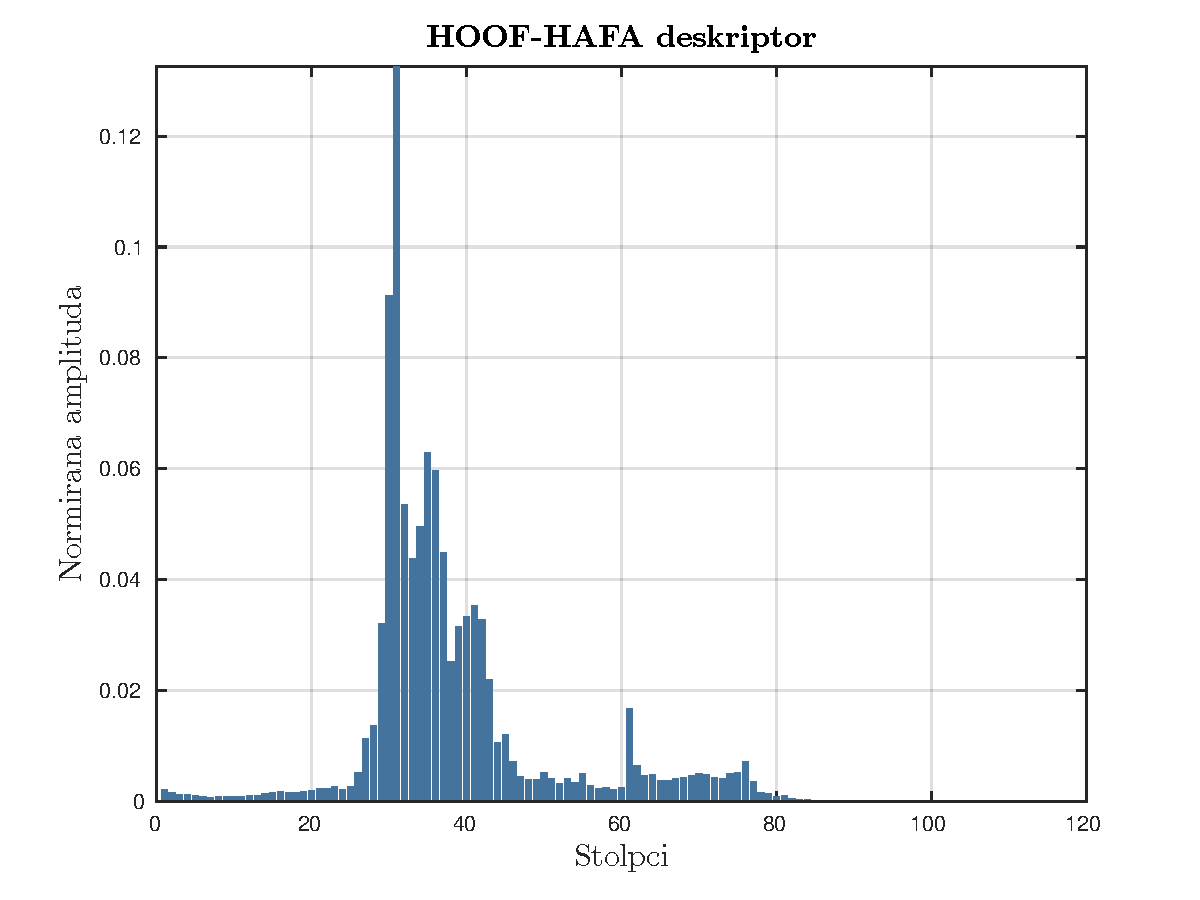
\includegraphics[width=0.6\columnwidth]{stage1-field-bv-of-hist-sl}
	\caption[HOOF-HAFA deskriptor za 276. sliko učnih vzorcev]{HOOF-HAFA deskriptor za 276. sliko učnih vzorcev. Deskriptor se ujema s sliko \ref{fig:sledenje-squash}.}
	\label{fig:hoof-hafa}
\end{figure}

\subsubsection{Postopek procesiranja}
Za določitev področja posameznega igralca smo uporabili KCF sledilnik. Kadar sledilnik ni uspel najti objekta zanimanja, je bilo področje prazno, zato so bile vse vrednosti HOOF-HAFA deskriptorjev $0$. To se je zgodilo v primerih, ko je tarča izginila iz vidnega polja kamere ali pa ko sledilnik ni več deloval. Zaradi teh težav smo sledenje nadzorovano reinicializirali vsake \SI{3}{\s}. S tem smo zagotovili razumne sledilne rezultate. Zaradi prevelike resolucije posnetkov, smo morali za pravilno delovanje sledilnika posnetke skalirati na \SI{25}{\%} prvotne velikosti. Rezultate sledenja smo nato morali transformirati nazaj na originalno resolucijo. Primer sledenja je prikazan na sliki \ref{fig:squash}\subref{fig:sledenje-squash})

\begin{figure}[!htb]
	\centering
	\begin{subfigure}[t]{0.45\columnwidth}
		\centering
		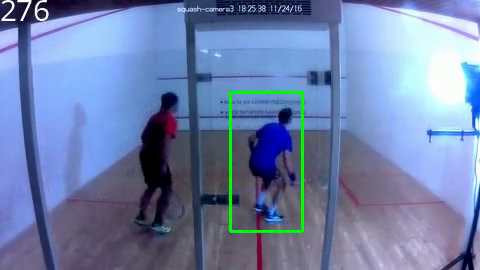
\includegraphics[width=\columnwidth]{squash-tracked.png}
		\caption{Slika sledenja.}
	    \label{fig:sledenje-squash}
	\end{subfigure}
	~
	\begin{subfigure}[t]{0.45\columnwidth}
		\centering
		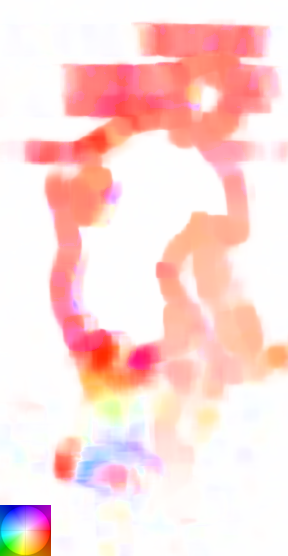
\includegraphics[width=0.4\columnwidth, frame]{stage1-squash-flo-corrected.png}
		\caption{Slika optičnega toka.}
		\label{fig:of-squash}
	\end{subfigure}
	\caption[Slika sledenja in optičnega toka za igralca terenskih eksperimentov]{Slika sledenja in optičnega toka za igralca prve igre terenskih eksperimentov. Sledili smo modremu igralcu, ki smo ga uporabili za učne vzorce. Zeleni okvir na sliki \subref{fig:sledenje-squash}) prikazuje področje detekcije 276. slike posnetka. Korespondečni optični tok področja je prikazan na sliki \subref{fig:of-squash} z legendo barvnega kodiranja v spodnjem levem kotu. Na sliki uporabljamo standardno barvno kodiranje, povzeto po \cite{baker2011database}. Maksimalna amplituda optičnega toka je na tej sliki znašala \SI{31}{ppf}. }
	\label{fig:squash}
\end{figure}

Izmerjeni srčni utrip smo filtrirali z Gaussovim filtrom s standardnim odklonom \num{16}. S tem smo preprečili učenje na šumnih podatkih. Srčni utrip je bil individualiziran na parametre učnega igralca s pretvorbo v energijsko porabo po enačbi \eqref{eq:charlot}. Rezultate smo nato z isto enačbo pretvorili nazaj v srčni utrip s parametri testnega igralca. S tem smo omogočili učenje na enem in testiranje na drugem igralcu. 

Po določevanju optičnega toka (slika \ref{fig:squash}), smo uporabili HOOF-HAFA deskriptorje, katerih značilke smo skalirali na intervalu $[-1,1]$. Učili smo s postopkom \esvr in jedrom RBF. Za terenske eksperimente Kalmanovega filtra nismo uporabili. Ker je bil Gaussov filter uporabljen pri predprocesiranju podatkov, smo enak filter uporabili tudi za filtriranje izhodov modela.

\begin{figure}[!htb]
	\centering
	\resizebox{\columnwidth}{!}{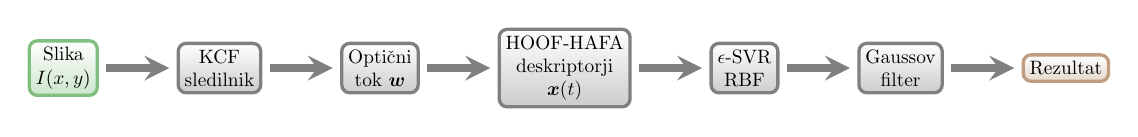
\begin{tikzpicture}
% LAYERS
\pgfdeclarelayer{bg}
\pgfsetlayers{bg,main}
\tikzset{
    between/.style args={#1 and #2}{
         at = ($(#1)!0.5!(#2)$)
    }
}

% NODES
\node (slika) [input] at (0,0) {Slika\\$I(x,y)$};
\node (tracker) [block, right= of slika] {KCF\\sledilnik};
%\node (tarca) [block, right= of tracker] {Področje\\tarče};

\node (of) [block, right= of tracker] {Optični\\tok $\vec{w}$};
\node (hoof) [block, right= of of] {HOOF-HAFA\\deskriptorji\\$\vec{x}(t)$};


\node (ucenje) [block, right=of hoof] {\esvr\\RBF};
\node (kalman) [block, right= of ucenje] {Gaussov\\filter};


\node (rezultat) [output, right= of kalman] {Rezultat};

% arrows
\draw [arrow] (slika) -- (tracker);
\draw [arrow] (tracker) -- (of);
%\draw [arrow] (tarca) -- (of);
\draw [arrow] (of) -- (hoof);
\draw [arrow] (hoof) -- (ucenje);
\draw [arrow] (ucenje) -- (kalman);
\draw [arrow] (kalman) -- (rezultat);
\end{tikzpicture}}
	\caption[Diagram procesiranja terenskih eksperimentov 1. faze]{Diagram procesiranja terenskih eksperimentov 1. faze. Področju, ki smo ga dobili s KCF sledinikom, smo določili optični tok. Sledilo je učenje na HOOF-HAFA deskriptorjih, Rezultate smo filtrirali s Gaussovim filtrom.}
	\label{fig:diagram-procesiranja-field-stag1}
\end{figure}

















\subsection{Detekcija dihanja}
Za prikaz splošne uporabnosti elementarnega postopka iz poglavja \ref{sec:elementarni-postopek}, smo ga uporabili za detekcijo dihanja. Za razliko od uporabe postopka v športu, lahko detekcijo dihanja uporabljamo za medicinske namene, v skrbi za starejše ali pri nadzornih kamerah. Koncept optičnega merjenja nam omogoča, da aplikacijo uporabimo z daljših razdalj, dokler nam optični sistem to omogoča. 

Seveda obstaja že kar nekaj aplikacij monitoringa pacientov s pomočjo računalniškega vida. Naša glavna motivacija je bilo testiranje predlagane metode na drugačnem problemu.

\subsubsection{Pridobivanje podatkov}
Za testiranje detekcije dihanja smo posneli video moškega merjenca, starosti 42 let z diagnozo spalne apneje. Snemanje se je začelo ob 4:45 zjutraj med spanjem merjenca in je trajalo 30 min. Prostor smo osvetlili z \SI{60}{w} bližnje-infrardečim (NIR) osvetljevalnikom. Snemali smo z RaspberryPi RaspiCam  napravo (NIR verzija, brez filtra za blokiranje NIR). Hitrost snemanja je bila \SI{25}{fps}, ki smo jo zmanjšali na \SI{10}{fps} v predprocesiranju videa. Ker je dihanje počasen proces, smo z zmanjševanjem hitrosti izboljšali SNR v pridobljenem optičnem toku. Pri snemanju smo uporabili širokokotno M12 lečo z goriščno razdaljo \SI{1.8}{mm}. Snemalna aparatura je bila oddaljena približno \SI{2}{m} od opazovanega subjekta. Primer slike posnetka je prikazan na sliki \ref{fig:dihanje-orig}.

\begin{figure}[htb]
	\centering
	\begin{subfigure}[t]{0.3\columnwidth}
		\centering
		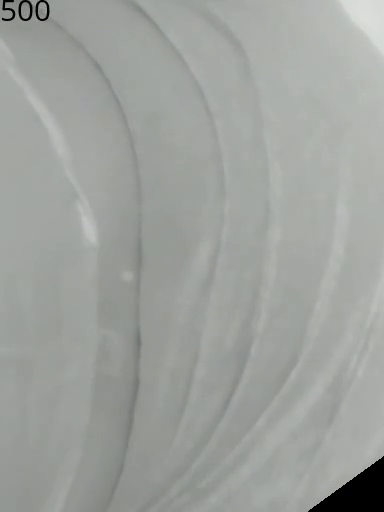
\includegraphics[width=\columnwidth]{breathtest-500.png}
		\caption{IR slika dihanja.}
		\label{fig:dihanje-orig}
	\end{subfigure}
	~
	\begin{subfigure}[t]{0.3\columnwidth}
		\centering
		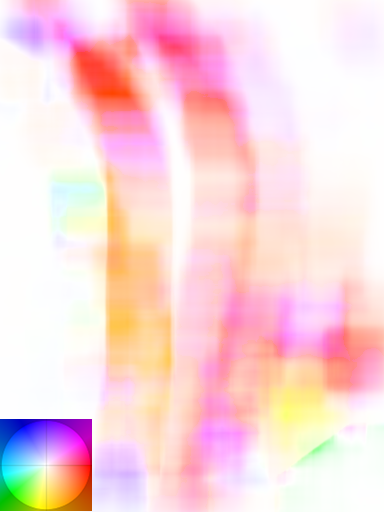
\includegraphics[width=\columnwidth, frame]{breathtest-flow-coding.png}
		\caption{Optični tok dihanja.}
		\label{fig:dihanje-of}
	\end{subfigure}
	~
	\begin{subfigure}[t]{0.3\columnwidth}
		\centering
		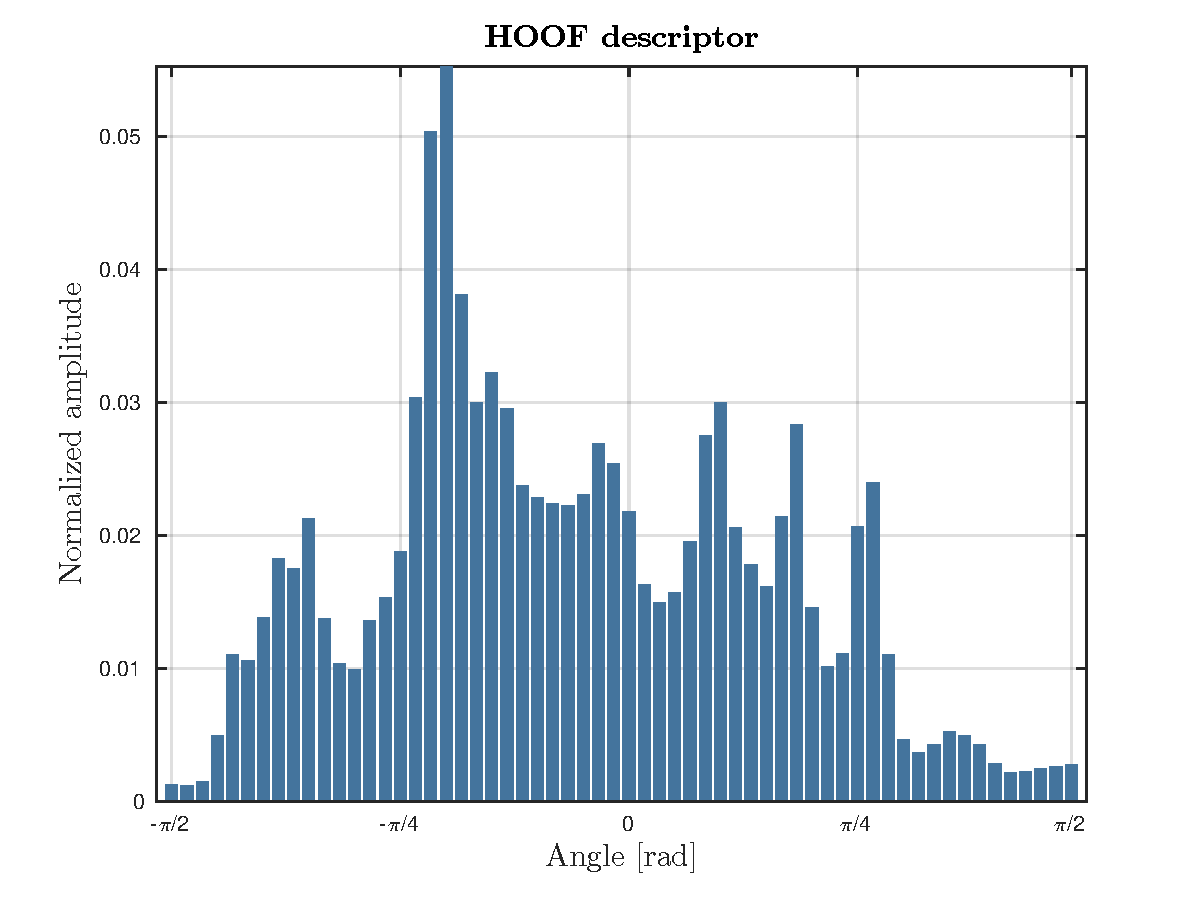
\includegraphics[width=\columnwidth]{stage1-breathtest-hist-en}
		\caption{HOOF histogram.}
		\label{fig:dihanje-hist}
	\end{subfigure}
	\caption[Originalna IR slika dihanja, njen optični tok in HOOF histogram]{Originalna IR slika dihanja, njen optični tok in HOOF histogram Prikazana je 500. slika učnih vzorcev. Optični tok ima z legendo barvnega kodiranja v spodnjem levem kotu. Na sliki uporabljamo standardno barvno kodiranje, povzeto po \cite{baker2011database}. Maksimalna amplituda optičnega toka je na tej sliki znašala \SI{1}{ppf}.}
	\label{fig:dihanje}
\end{figure} 

\subsubsection{Referenčni podatki}
Za pridobitev referenčnih podatkov smo snemali tudi zvok z avdio modulom za RaspberryPi. Mikrofon smo postavili v neposredno bližino merjenca. Zvok smo sinhronizirali z video posnetkom. Detekcije dihanja so predstavljale visoko amplitudo zvoka. Dobljene detekcije smo pregledali z operaterjem in potrdili, da korespondirajo z dejanskim dihanjem na avdio posnetku. Detekcije dihanja smo prevzorčili na \SI{10}{Hz}, da so se skladale s frekvenco vzorčenja video posnetka.

\subsubsection{Procesiranje}\label{sec:data-preprocessing}
Opazovali smo področje subjektovega hrbta. Subjekt je ležal obrnjen navzdol. Področje je bilo veliko $384 \times 512$ slikovnih elementov in je pokrivalo približno $2/3$ hrbta. To je bil edini del slike, ki smo ga uporabili.

Iz posnetka smo izbrali dva zaporedja slik s trajanjem \SI{5}{min}. Prvo zaporedje smo uporabili za učenje, drugo pa za testiranje. Pri uporabi optičnega toka smo spremenili parameter velikost okna na $64$. Iz optičnega toka smo izračunali HOOF histograme. Njihove značilke smo normirali na intervalu $[-1,1]$. Učili smo z C-SVC razvrščevalnikom in RBF jedrom, pri tem pa uporabili optimizacijo parametrov. Za določitev uspešnosti delovanja smo problem formulirali kot problem binarnega razvrščanja z razredoma ``diha'' in ``ne diha''. Rezultatov nismo filtrirali.

\begin{figure}[htb]
	\centering
	\resizebox{\columnwidth}{!}{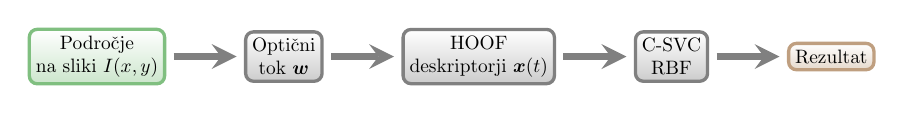
\begin{tikzpicture}
% LAYERS
\pgfdeclarelayer{bg}
\pgfsetlayers{bg,main}
\tikzset{
	between/.style args={#1 and #2}{
		at = ($(#1)!0.5!(#2)$)
	}
}

% NODES
\node (slika) [input] at (0,0) {Področje\\na sliki $I(x,y)$};

\node (of) [block, right= of slika] {Optični\\tok $\vec{w}$};
\node (hoof) [block, right= of of] {HOOF\\deskriptorji $\vec{x}(t)$};


\node (ucenje) [block, right= of hoof] {C-SVC\\RBF};

\node (rezultat) [output, right= of ucenje] {Rezultat};

% arrows
\draw [arrow] (slika) -- (of);


\draw [arrow] (of) -- (hoof);
\draw [arrow] (hoof) -- (ucenje);

\draw [arrow] (ucenje) -- (rezultat);
\end{tikzpicture}}
	\caption[Diagram procesiranja pri uporabi metode za detekcijo dihanja]{Diagram procesiranja pri uporabi metode za detekcijo dihanja.}
	\label{fig:dihanje-postopek}
\end{figure}

% \begin{table}[h]
%     \centering
%     \begin{tabular}{l r D{.}{.}{-1} D{.}{.}{-1}}
% 		\toprule
%         \textbf{Model name} & \multicolumn{3}{c}{\textbf{Parameters}} \\
%         & \multicolumn{1}{c}{$C$} & \multicolumn{1}{c}{$\gamma$} & \multicolumn{1}{c}{$\epsilon$} \\
%         \midrule
%         hr-sv		&	1024	&	16	&	3.48	\\
%         hr-sv-lag 	&	4096	&	11.31
%         &	2.14	\\
%         hr-bv		&	4096	&	16	&	4.59	\\      
%         hr-bv-lag 	&	1024	&	16	&	2.46	\\
%         eem-sv		&	256	&	16	&	0.81	\\
%         eem-sv-lag	&	256	&	16	&	0.54	\\
%         eem-bv		&	256	&	16	&	1.62	\\   
%         eem-bv-lag	&	256	&	16	&	1.74	\\
%         hr-mixed	&	1024	&	16	&	4.59	\\
%         hr-mixed-lag &	1024	&	16	&	4.59	\\
%         eem-mixed	&	90.51	&	16	&	1.15	\\
%         eem-mixed-lag	&	64	&	16	&	0.93	\\
%         hr-sv-tr	&	1024	&	11.31	&	3.73	\\
%         hr-sv-lag-tr	&	1024	&	16	&	3.03	\\
%         hr-bv-tr	&	256	&	16	&	2.64	\\
%         hr-bv-lag-tr	&	256	&	16	&	3.48	\\
%         eem-sv-tr	&	256	&	11.31	&	0.50	\\
%         eem-sv-lag-tr	&	256	&	16	&	0.31	\\
%         eem-bv-tr	&	64	&	16	&	1.87	\\
%         eem-bv-lag-tr	&	64	&	16	&	1.87	\\
%         hr-sv-tr-sh	&	64	&	16	&	4.59	\\
%         hr-sv-lag-tr-sh	&	64	&	16	&	4.59	\\
%         hr-bv-tr-sh	&	16	&	16	&	1.23	\\
%         hr-bv-lag-tr-sh	&	16	&	11.31	&	2.14	\\
%         eem-sv-tr-sh	&	16	&	16	&	0.62	\\
%         eem-sv-lag-tr-sh	&	16	&	16	&	0.87	\\
%         eem-bv-tr-sh	&	1.41	&	16	&	0.09	\\
%         eem-bv-lag-tr-sh	&	4	&	16	&	1.23	\\
%         hr-bv-lag-tr-sq	&	1024	&	0.25	&	4.59	\\
%         \bottomrule
% 	\end{tabular}
%      \caption{The optimal parameters for individual models, which were obtained by grid search with five-fold cross-correlation, as indicated in \cite{hsu2003practical}. Parameters were used for learning models with the LIBSVM library.}
%     %\caption{Optimalni parametri za posamezne modele, ki smo jih dobili z mrežnim iskanjem s petkratno križno korelacijo, kot je navedeno v \cite{hsu2003practical}. Parametre smo uporabili za učenje modelov v knjižnici LIBSVM.}
%     \label{tab:optimalni-parametri}
% \end{table}

% As said in \ref{sec:data-preprocessing}, predicted results for squash experiment were converted with basic equation from \cite{charlot2014improvement}, because energy expenditure models were used.


\section{Eksperimenti 2. faze}
Z laboratorijskimi eksperimenti v 1. fazi smo dobili zadovoljive rezultate, težave pa so nastale pri uporabi postopka na terenu. Zato smo v 2. fazi optimizirali posamezne segmente elementarnega postopka estimacije fizioloških parametrov. Te smo tudi uporabili v končni preiskavi. V preliminarnih testih so opisani tudi drugi postopki, ki smo jih potrebovali zaradi uporabe Kinect kamer.

Za statistično bolj oprijemljive rezultate smo v laboratorijskih in terenskih eksperimentih 2. faze uporabili 7 različnih merjencev z oznakami: SUBJ1, SUBJ2, SUBJ4, SUBJ7, SUBJ8, SUBJ9, SUBJ10. 

Merjenca SUBJ4 smo uporabili samo v laboratorijskih eksperimentih, ker pri terenskih eksperimentih ni bil prisoten. Namesto njega smo v terenskih eksperimentih uporabili merjenca SUBJ10. V laboratorijskih eksperimentih merjenca SUBJ10 nismo upoštevali zaradi napak pri zajemu meritev.

Med laboratorijskimi in terenskimi eksperimenti je za merjenca SUBJ1 in SUBJ2 preteklo 43 dni, za merjenca SUBJ4 42 dni in za ostale 1 dan.  

\subsection{Preliminarni testi}
\subsubsection{Združevanje slik iz dveh Kinect kamer}\label{sec:zdruzevanje}

\paragraph{Združevanje z značilkami}
Časovno sinhornizirana zaporedja slik smo poskušali združiti z metodo panoramskega šivanja slik z uporabo značilk, kot je opisano v delu \cite{brown2007automatic}. Tu smo namesto SIFT značilk uporabili SURF značilke.


\paragraph{Združevanje s kontrolnimi točkami}
Zaporedja slik smo poskušali združiti z ročnim določevanjem kontrolnih točk.


\paragraph{Prilagojeno združevanje}
Zaradi nezadovoljivih rezultatov klasičnih metod združevanja stereo slik, smo razvili metodo, ki je prilagojena za Kinect kamere. Iz kamer smo pridobili intrinzične parametre infra-redečega (IR) senzora, in sicer: slikovni koordinati goriščne razdalje $f_u$ in $f_v$ ter slikovni koordinati optičnega središča slike (ang. principal point) $c_u$ in $c_v$. Intrinsične parametre smo uporabili za določitev intrizične matrike $\vec{M}_{int}$ po enačbi \eqref{eq:intrinsic}.


Ker pravih ekstrinsičnih parametrov kamer nismo poznali, smo jih le ocenili z metodo določevanja sečišča vidnih polj obeh kamer. Sečišče je prikazano kot rdeča linija na sliki \ref{fig:zdruzevanje}. S to metodo smo določili translacijski vektor $\vec{t} = \left [ t_x~ t_y~ t_z \right]^\top$ in rotacijsko matriko $\vec{R}$ iz Eulerjevih kotov.

S sledenjem igralca z DS-KCF algoritmom, smo s pomočjo projekcijske matrike \eqref{eq:projection-matrix} določili center tarče v metričnih enotah za vsako sliko zaporedja leve in desne kamere. Kadar slikovni element ni vseboval podatkov globine, smo za center tarče izbrali najbližji slikovni element z veljavno globino.

Prva slika združenega zaporedja je bila slika kamere, kjer se igralec prvič pojavi. Nadaljne slike smo izbirali med zaporedjema kamer glede na pozicijo centra tarče. Ko je šel center tarče skozi upragovljeno mejo, ki je na sliki \ref{fig:zdruzevanje} prikazana z modro linijo smo preklopili na drugo kamero. Razdalja med pragom in sečiščem je znašala \SI{200}{mm}.


\begin{figure}[htb]
	\centering
	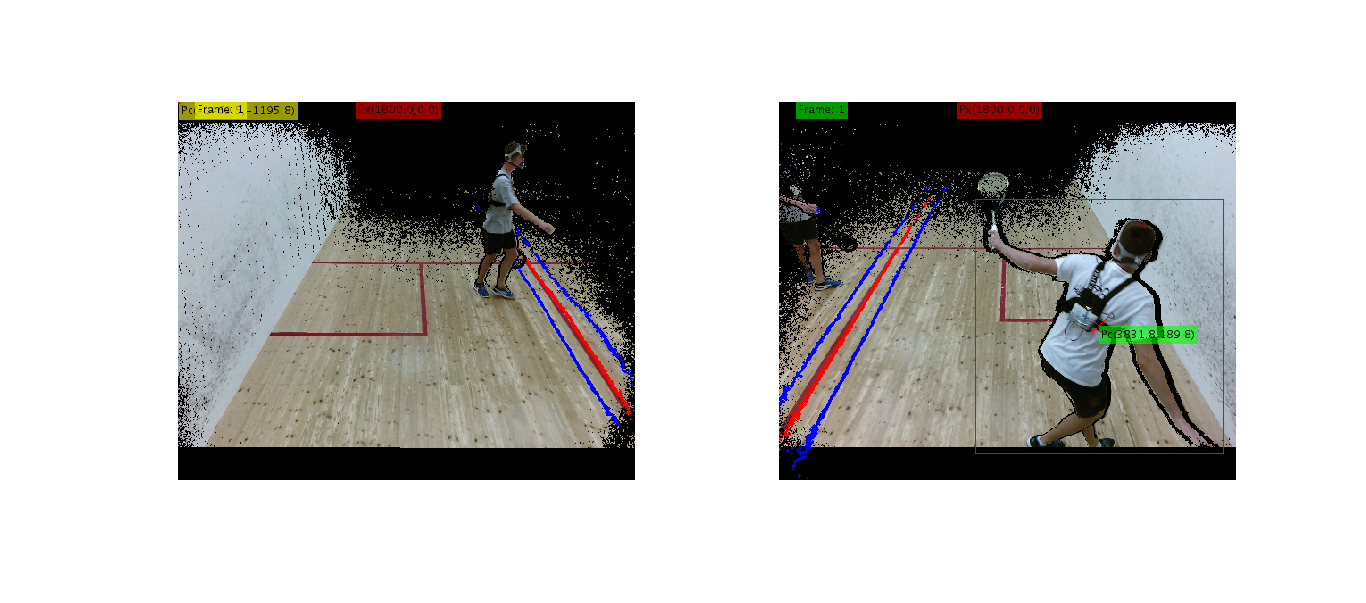
\includegraphics[width=\columnwidth]{./Slike/zdruzevanje-example.png}
	\caption[Določevanje sečišča vidnih polj leve in desne Kinect kamere]{Določevanje sečišča vidnih polj leve in desne Kinect kamere. Na sliki sta prikazani prvi sliki zaporedja leve in desne Kinect kamere 1. seta 2. igre terenskega eksperimenta iz 2. faze. Označen je 4. igralec. Zelena barva koordiat središča tarče predstavlja izbrano kamero. Kamera z rumeno barvo ni izbrana. Sečišče je rdeča linija. Modri liniji sta pragova za preklop med kamerama. Ležita \SI{200}{mm} levo in desno od sečišča.}
	\label{fig:zdruzevanje}
\end{figure}



\subsubsection{Mrežno iskanje \texorpdfstring{$\nu$}{nu}-RBF}
Med evaluacijo eksperimentov 1. faze smo ugotovili, da z regresijo \esvr pogosto dobimo preobremenjene (ang. Overfitted) modele. Pri takih modeli je število podpornih vektorjev zelo visoko. Lahko se zgodi, da postanejo vsi vektorji značilk podporni vektorji. Preobremenjeni modeli lahko dajejo solidne rezultate, vendar pa so ti nerealistični. Takoj, ko bi v tak model vnesli rahlo spremenjene podatke, ne bi več delovali.

Zaradi tovrstnih problemov smo v našem postopku regresijo \esvr zamenjali z \nusvr. Izkazalo se je, da tudi ta ne deluje, čeprav pri njej uporabljamo dodatni parameter $\nu$, s katerim v teoriji kontroliramo razmerje števila podpornih vektorjev, kot je opisano v poglavju \ref{sec:regresija-nusvr}. Chang et. al nam v delu \cite{chang2002training} parameter $\nu$ bolj natačno opiše kot spodnjo mejo razmerja števila podpornih vektorjev. Parameter $\nu$ tako v resnici ne predstavlja omejitve, s katero bi kaznovali prekomerno učneje modela. V ta namen smo razvili mrežno iskanje \nurbf, ki je predstavljeno v poglavju \ref{sec:nurbf}. 

Razvito mrežno iskanje \nurbf uporablja regresijo \nusvr in jedro RBF, zato smo ju uporabljali tudi za učenje modelov. Celoten postopek krajše imenujemo kar \nurbf.

\paragraph{Optimizacija parametrov}
Najprej smo optimizirali parameter $\numax$ oziroma $\numax'$. Slednji predstavlja različico parametra $\numax$, s katerim določimo dejansko število podpornih vektorjev. Za tovrstno optimizacijo smo ponovno naučili \textit{mixed} modele iz 1. faze, pri čemer smo za mrežno iskanje uporabili nov postopek. Modele smo nato uporabili za testiranje na učnih podatkih terenskih eksperimentov 1. faze. S takim postopkom smo izluščili slabe \textit{squash} modele, ki bi oteževali pravilno evaluacijo rezultatov pri optimizaciji.

Za optimizacijo smo uporabili HOOF-HAFA deskriptor in naslednje vrednosti parametrov: začetna vrednost $\nu$ $0.1$ in standardni odklon za Gaussov filter $\sigma=5$. Za $\numax'$ smo uporabili 400, 800 in 1200 podpornih vektorjev. 

Z optimiziranim parametrom $\numax'=400$ smo \nurbf preizkusili še na elementarnih modelih. Tu smo za razliko od eksperimentov iz 1. faze poleg \nurbf uporabili razširjeni HOOF-HAFA deskriptor.







\subsubsection{Jedro GHI}
V poglavju \ref{sec:ghi} smo opisali, da je jedro GHI primerno za histogramske deskriptorje, zato smo ga tudi preizkusili na elementarnih modelih. Tu smo namesto prvotnega HOOF deskriptorja uporabili HOOF-HAFA deskriptor, ki daje boljše rezultate. Pri uporabi GHI jedra smo značilke skalirali na intervalu $[-1,~1]$ zaradi hitrejšega učenja. Učili smo z \esvr metodo. Rezultate smo filtrirali s prvotnim Kalmanovim filtrom.

Zaradi že prej omenjenih težav s prevelikim številom podpornih vektorjev v modelih, smo pri klasičnem mrežnem iskanju sprva uporabili enostavno mero: faktor števila podpornih vektorjev $f_{nSV}$, ki je opisan z enačbo \eqref{eq:fnsv}. $n_v$ je število vzorcev in $n_{SV}$ je število podpornih vektorjev. S to mero določimo procentualno vrednost vektorjev, ki lahko postanejo podporni. Zaradi tega faktorja optimizacija parametra regresije ni bila potrebna. Pri testiranju smo uporabili vrednost $f_{nSV} = 0.01$.


\begin{equation}
f_{nSV} = \frac{n_v - n_{SV}}{n_v}
\label{eq:fnsv}
\end{equation} 

Zgoraj opisana metoda ni delovala zato smo namesto faktorja $f_{nSV}$ uporabili postopek \nughi. Gre za prilagojeno različico postopka \nurbf, kjer smo uporabili GHI jedro. Dodatna razlika je še v tem, da predikcij pri križni validaciji nismo filtrirali, ker smo pri rezultatih uporabili Kalmanov filter. Prav tako smo s tem zagotovili zadovoljiv čas reševanja problema.






\subsubsection{Optimizacija Gaussovega filtra}
Pri optimizaciji Gaussovega filtra smo določili optimalni standardni odklon $\sigma$ z uporabo dveh metrik, in sicer: koren srednje kvadratične napake (RMSE) in razmerje med signalom in šumom (SNR). Pri RMSE metriki smo določili napako med učnimi vzorci in njihovo predikcijo. Pri SNR metriki smo za signal uporabili referenčne učne vzorce. Za šum smo uporabili rezidualni ali preostali šum. Tega smo dobili z odštevanjem filtriranih vzorcev od referenčnih. SNR metrika tako določa uspešnost izločevanja šuma, RMSE metrika pa pravilnost določevanja kateri podatki spadajo v signal in kateri v šum.


Teste smo izvajali na vseh eksperimentih 1. sklopa, pri čemer smo uporabili \nurbf mrežno iskanje s \SI{50}{\%} podpornih vektorjev. Za filtriranje pri mrežnem iskanju smo izbrali najmanjši filter s $\sigma = 1$. Testirali smo naslednje standardne odklone Gaussovega filtra: $1, 3, 5, 11, 21, 31$ in $51$. 




\subsubsection{Normalizacija HAFA deskriptorjev}
V praksi se pokaže, da prvotni HAFA histogram ne deluje zadovoljivo, saj se histogram lahko močno spreminja pri uporabi sledilnika. Zaradi neidelanega delovanja sledilnika področje tarče skozi čas spreminja svojo velikost, to pa vpliva na vrednosti stolpcev HAFA histograma. Ker te dobimo s preštevanjem slikovnih elementov z enako amplitudo hitrosti bo manjše področje posledično zmanjšalo celoten histogram. Pri HOOF histogramih tega problema praktično nimamo, saj ima majhen vpliv. Razlog tiči v računanju vrednosti stolpcev HOOF histograma. Njihove vrednosti dobimo s seštevanjem amplitud in ne njihovim preštevanjem. Te so zato pred normiranjem praviloma večje.

Probleme sledilnika smo poskušali kompenzirati z uvedbo amplitudnega faktorja $f_A$. Amplitudni faktor je pravzaprav razmerje med velikostjo področja igralca na terenskih testih in velikostjo merjenca na tekalni stezi. Razmerje lahko preprosto dobimo z razmerjem diagonal področij po enačbi \eqref{eq:diag}, kjer so $w_l$ in $h_l$ širina in dolžina področja na tekalni stezi ter $w_s$ in $h_s$ širina in dolžina področja na terenskih testih.

\begin{equation}
f_A = \frac{\sqrt{w_l^2 + h_l^2}}{\sqrt{w_s^2 + h_s^2}}
\label{eq:diag}
\end{equation}

Velikost diagonale na laboratorijskih testih uporabljamo kot referenco. To pa zato, ker je na teh posnetkih stabilna, saj se le malo spreminja. Koncept amplitudnega faktorja smo preizkusili na enakem postopku, kot pri optimizaciji parametra mrežnega iskanja \nurbf. S takim postopkom smo izluščili slabe \textit{squash} modele, ki bi oteževali pravilno evaluacijo rezultatov pri optimizaciji. Naučili smo modele \textit{diag}, kjer smo uporabili amplitudni faktor in referenčne modele \textit{normal} brez uporabe faktorja za primerjavo. Diagonalo na tekalni stezi smo določili po sliki \ref{fig:diag-bbox}, kjer smo za zgornji levi kot $P_0$ in spodnji desni kot $P_1$ izbrali vrednosti v tabeli \ref{tab:diag}. 


\begin{figure}[htb]
	\centering
	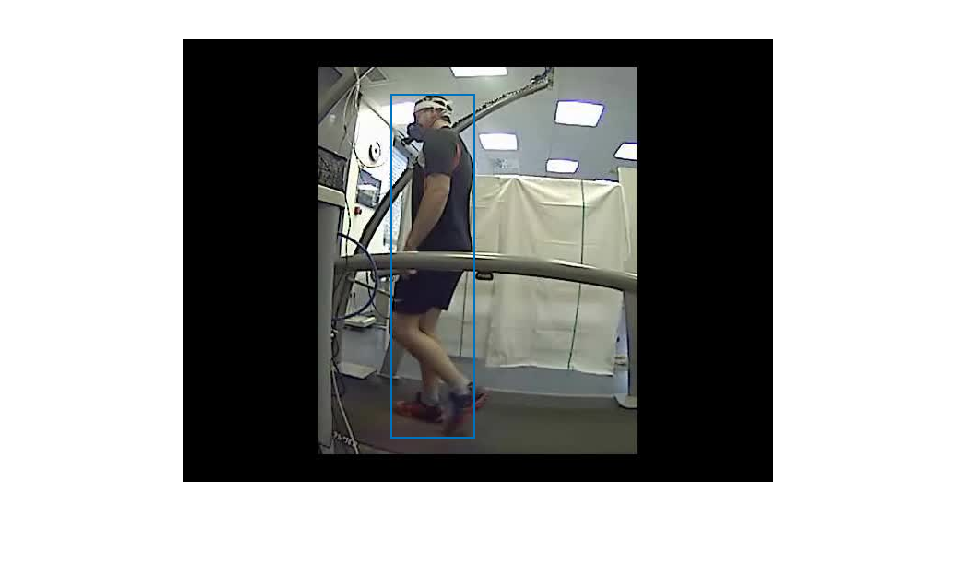
\includegraphics[width=0.75\columnwidth]{./Slike/diag-bbox.png}
	\caption{}
	\label{fig:diag-bbox}
\end{figure}

\begin{table}[htb]
	\centering
	\begin{tabular}{l S[table-format=3] S[table-format=3]}
		\toprule
		\textbf{Točka} & \thead{$\mathbf{x}$} & \thead{$\mathbf{y}$} \\ 
		\midrule
		$P_0$ & 297 & 82 \\
		$P_1$ & 389 & 452 \\
		\bottomrule
	\end{tabular}
	\caption[Optimalni parameteri RBF jedra modelov za izbiro deskriptorjev]{Optimalni parametri RBF jedra za modele z različnim deskriptorjem.}
	\label{tab:diag}
\end{table}

Pri testiranju smo uporabili parameter $\numax$ \SI{50}{\%} podpornih vektorjev. Za Gaussov filter smo uporabili $\sigma=5$. Značilke smo skalirani na intervalu $[0,~1]$. Za modele z diagonalo smo uporabili parameter $f_{A}=381.266$. Pri učenju smo uporabili optimalne vrednosti parametrov, ki so prikazane v tabeli \ref{tab:diag}. Za evaluacijo rezultatov smo uporabili predikcije testnih vzorcev z modeli s zakasnitvijo.



\begin{table}[htb]
	\centering
	\begin{tabular}{l S[table-format=3] S[table-format=1.3] S[table-format=1.1] S[table-format=1.3]}
		\toprule
		\textbf{Model} & \thead{$\mathbf{C}$} & \thead{$\mathbf{\gamma}$} & \thead{$\mathbf{\nu}$} & \thead{MSE} \\ 
		\midrule
		NORMAL & 256 & 0.354 & 0.1 & 5.297 \\
		DIAG & 256 & 0.354 & 0.1 & 5.297 \\
		\bottomrule
	\end{tabular}
	\caption[Optimalni parameteri RBF jedra modelov za izbiro deskriptorjev]{Optimalni parametri RBF jedra za modele z različnim deskriptorjem.}
	\label{tab:izbira-param-diag}
\end{table}


\subsection{Laboratorijski eksperimenti}
Merjenci so opravili obremenilni test po protokolu Nowatzky. To je stopnjevani test na tekoči preprogi za merjenje maksimalne porabe kisika in oceno aerobne kapacitete posameznika. Test smo izvajali s pomočjo sistema za direktno ergospirometrijo tipa ``breath  by breath'' Cosmed K4B2. Uporabili smo  tekočo  preprogo HP Cosmos.

\subsubsection{Pridobivanje podatkov}
Tekalno stezo smo snemali iz dveh različnih zornih kotov: hrbtni del in stranski del.  Primer hrbtnega in stranskega posnetka je prikazan na sliki \ref{fig:primer-posnetka-stage2}.

\begin{figure}[htb]
	\centering
	\begin{subfigure}{0.45\columnwidth}
		%\includegraphics[width=\columnwidth]{./Slike/normal-sv-150.png}
		\caption{stranska slika}
	\end{subfigure}
	~
	\begin{subfigure}{0.45\columnwidth}
		%\includegraphics[width=\columnwidth]{./Slike/normal-bv-150.png}
		\caption{hrbtna slika}
	\end{subfigure}
	\caption{Hrbtna in stranska 150. slika RGB posnetkov iz prve serije.}
	\label{fig:primer-posnetka-stage2}
\end{figure}

Snemali smo z dvema Microsoft Xbox Kinect V2 kamerama. Kameri sta bili od tekalne steze oddaljeni približno \SI{2}{m}. Od tal sta bili dvignjeni za približno \SI{1.5}{m}. Pridobili smo barvne RGB in globinske DEPTH slike. Snemali smo v ločljivosti $512 \times 424$. Hitrost posnetkov je znašala \SI{30}{fps}. Kameri smo časovno sinhronizirali po NTP protokolu.

Z obremenilnim testom smo pridobili podatke enrgijske porabe šestih različnih merjencev z oznakami: SUBJ1, SUBJ2, SUBJ4, SUBJ7 SUBJ8 in SUBJ9. Vzorčili smo s frekvenco \SI{0.2}{\hertz}.

\subsubsection{Protokol izvajanja meritev}
Test smo pričeli z eno minutnim mirovanjem na tekalni stezi. Sledilo je tri minutno ogrevanje s hitrostjo teka \SI{5}{\km\per\hour}, pri naklonu preproge \SI{0}{\%}. Nadaljevali smo s 3 minutnim tekom s hitrostjo \SI{6}{\km\per\hour}. Po treh minutah smo naklon tekoče preproge  dvignili za \SI{2}{\%} in ga nismo več spreminjali. Po pretečeni minuti na  tretji stopnji (hitrost \SI{6}{\km\per\hour}, naklon \SI{2}{\%}) se je hitrost teka vsaki dve  minuti  povečevala za \SI{1}{\km\per\hour}. Test smo izvajali brez prekinitve do pojava objektivnih oz. subjektivnih razlogov za prekinitev testa. 
%Po koncu testiranja je sledilo še \SI{5}{min} hoje pri  hitrosti \SI{2}{\km\per\hour} ter \SI{0}{\%} naklonu. 
 

\subsubsection{Protokoli postopka procesiranja}
Tako kot pri eksperimentih 1. faze so bile  meritve fizioloških parametrov izvedene z vzorčenjem \SI{0.2}{\hertz}, hitrost posnetkov pa je bila \SI{30}{fps}. Zaradi neskladja frekvenc vzorčenja, smo te interpolirali s pomočjo Matlabove funkcije \texttt{interp1}.

Tokrat smo modele učili po dveh postopkih. Prvi postopek temelji na optičnem toku, drugi pa na prostorskem.

\paragraph{Postopek z optičnim tokom}
Na slikah posnetkov smo merjencem sledili s sledilnikom KCF. Za tako izbrano področje slike smo izračunali optični tok. Primer dobljenega optičnega toka je prikazan na sliki \ref{fig:opticni-tok-stage2}. Sledilo je generiranje HOOF-HAFA deskriptorjev s parametri $N_{HOOF} = 60$ in $N_{HAFA} = 60$. HAFA deskriptorje smo normalizirali z vrednostmi amplitudnih faktorjev $f_A$, ki so zbrani v tabeli \ref{tab:fa-merjenci}.

\begin{figure}[htb]
	\label{fig:opticni-tok-stage2}
\end{figure}

\begin{table}[htb]
	\centering
	\begin{tabular}{l l S[table-format=3.3]}
		\toprule
		\textbf{Pogled} & \textbf{Merjenec} & \thead{$\mathbf{f_A}$} \\
		\midrule
		\multirow{7}{*}{hrbtni}
		&1&208.557\\
		&2&179.011\\
		&4&225.568\\
		&7&195.133\\
		&8&209.991\\
		&9&182.003\\
		&10&207.002\\
		\midrule
		\multirow{7}{*}{stranski}
		&1&236.985\\
		&2&163.957\\
		&4&196.461\\
		&7&205.760\\
		&8&190.253\\
		&9&178.16\\
		\bottomrule
	\end{tabular}
	\caption[Faktor amplitud za posamezne merjence pri različnem pogledu]{Faktor amplitud za posamezne merjence pri različnem pogledu.}
	\label{tab:fa-merjenci}
\end{table}

\begin{figure}[htb]
	\centering
	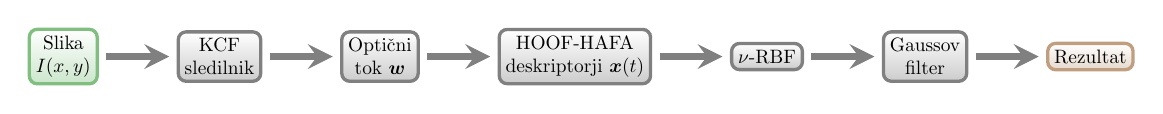
\begin{tikzpicture}
% LAYERS
\pgfdeclarelayer{bg}
\pgfsetlayers{bg,main}
\tikzset{
    between/.style args={#1 and #2}{
         at = ($(#1)!0.5!(#2)$)
    }
}

% NODES
\node (slika) [input] at (0,0) {Slika\\$I(x,y)$};
\node (tracker) [block, right= of slika] {KCF\\sledilnik};
%\node (tarca) [block, right= of tracker] {Področje tarče};

\node (of) [block, right= of tracker] {Optični\\tok $\vec{w}$};
\node (hoof) [block, right= of of] {HOOF-HAFA\\deskriptorji $\vec{x}(t)$};


\node (ucenje) [block, right=of hoof] {\nurbf};
\node (kalman) [block, right= of ucenje] {Gaussov\\filter};


\node (rezultat) [output, right= of kalman] {Rezultat};

% arrows
\draw [arrow] (slika) -- (tracker);
\draw [arrow] (tracker) -- (of);
%\draw [arrow] (tarca) -- (of);
\draw [arrow] (of) -- (hoof);
\draw [arrow] (hoof) -- (ucenje);
\draw [arrow] (ucenje) -- (kalman);
\draw [arrow] (kalman) -- (rezultat);
\end{tikzpicture}
	\caption{Diagram postopka procesiranja z optičnim tokom za eksperimente 2. faze.}
	\label{fig:diagram-procesiranja-of-stage2}
\end{figure}

\paragraph{Postopek s prostorskim tokom}
Na slikah posnetkov smo merjencem sledili s sledilnikom DS-KCF. Za tako izbrano področje slike smo izračunali prostorski tok. Primer dobljenega optičnega toka je prikazan na sliki \ref{fig:prostorski-tok-stage2}. Sledilo je generiranje HOOF-HAFA deskriptorjev s parametri $N_{HOOF} = 60$ in $N_{HAFA} = 60$. HAFA deskriptorjev  nismo normalizirali, ker smo histograme pridobili iz podatkov z metričnimi enotami. 

\begin{figure}[htb]
	\label{fig:prostorski-tok-stage2}
\end{figure}

\begin{figure}[htb]
	\centering
	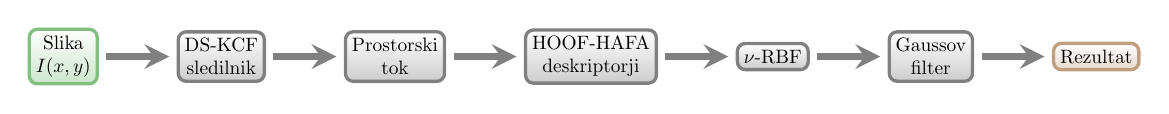
\begin{tikzpicture}
% LAYERS
\pgfdeclarelayer{bg}
\pgfsetlayers{bg,main}
\tikzset{
	between/.style args={#1 and #2}{
		at = ($(#1)!0.5!(#2)$)
	}
}

% NODES
\node (slika) [input] at (0,0) {Slika\\$I(x,y)$};
\node (tracker) [block, right= of slika] {DS-KCF\\sledilnik};
%\node (tarca) [block, right= of tracker] {Področje\\ tarče $x^{p}$};

\node (of) [block, right= of tracker] {Prostorski\\ tok};
\node (hoof) [block, right= of of] {HOOF-HAFA\\deskriptorji};


\node (ucenje) [block, right=of hoof] {\nurbf};
\node (kalman) [block, right= of ucenje] {Gaussov\\ filter};


\node (rezultat) [output, right= of kalman] {Rezultat};

% arrows
\draw [arrow] (slika) -- (tracker);
\draw [arrow] (tracker) -- (of);
%\draw [arrow] (tarca) -- (of);
\draw [arrow] (of) -- (hoof);
\draw [arrow] (hoof) -- (ucenje);
\draw [arrow] (ucenje) -- (kalman);
\draw [arrow] (kalman) -- (rezultat);
\end{tikzpicture}
	\caption{Diagram postopka procesiranja s prostorskim tokom za eksperimente 2. faze.}
	\label{fig:diagram-procesiranja-sf-stage2}
\end{figure}
 
Modele obeh postopkov smo učili s postopkom \nurbf, kjer smo za Gaussov filter uporabili $\sigma=5$ in za največje število podpornih vektorjev $\numax =0.5$ (\SI{50}{\%} podpornih vektorjev). Podobno kot v eksperimentih 1. faze smo tudi tu naučili \num{6} elementarnih modelov, in sicer: \textit{eem} modele, ki predvidevajo porabo energije v \si{\kcal\per\min}, \textit{sv} modele za stransko kamero in \textit{bv} modele za hrbtno kamero ter \textit{lag} modele z upoštevanjem časovne zakasnitve.

Vse tipe eksperimentov smo križno testirali glede na enak tip eksperimenta, le z drugim zornim kotom kamere. Uporabljen zorni kot kamere za križno testiranje je v imenih modelov zapisan v oklepajih.  Rezultate smo filtrirali z Gaussovim jedrom $\sigma=5$. 

Modele smo testirali po treh različnih protokolih. S prvim protokolom smo preverjali neodvisnost od časovnega povečevanja porabe, z drugim pa ravno obratno. S tretjim protokolom smo želeli pokazati delovanje posplošenega modela na različnih merjencih.


\paragraph{Protokol 1.}
Za testne vzorce vzamemo vsak 3. vzorec fiziološkega parametra in slike iz posameznega posnetka. Ostale vzorce uporabimo pri učenju. Rezultate vseh 6 meritev povprečimo.

\paragraph{Protokol 2.}
Za učne vzorce izberemo prvih \SI{70}{\%} vzorce in za testne naslednjih \SI{30}{\%}. Rezultate vseh 6 meritev povprečimo.

\paragraph{Protokol 3.}
Uporabimo protokol 1, pri čemer učimo na prvih štirih meritvah in testiramo na zadnjih dveh. Rezultata povprečimo.

\subsubsection{Določitev zakasnitve fiziološkega odziva}
Določitve zakasnitve fiziološkega odziva smo se, glede na eksperimente 1. faze, tu lotili nekoliko drugače. Na podlagi protokola izvajanja meritev, smo pridobili podatke eno minutnega mirovanja posameznega merjenca z vzorčno frekvenco \SI{0.2}{\hertz}. Kljub temu, da je signal v stacionarnem stanju, je nihajoč zaradi narave fiziologije. Signal mirovanja smo interpolirali na vzorčno frekvenco \SI{1}{\hertz}. Določili smo mu srednjo vrednost in vrednost treh standardnih odklonov. S tem smo dobili interval nedoločenosti, v katerem ne moremo določiti ali je pri spremembi amplitude signala prišlo zaradi fizioloških dejavnikov ali zaradi dejanskega odziva na vzbujalni signal. 

Na podlagi slik \ref{fig:lag-estimation-stage2}, smo zakasnitev za posamezno meritev določili kot časovni interval od trenutka spremembe hitrosti tekalne steze do trenutka, ko je bila vrednost fiziološkega parametra prvič nad intervalom nedoločenosti. Zakasnitev smo, zaradi treh standardnih odklonov, lahko določili s \SI{99.73}{\%} zagotovostjo za posameznega merjenca. Zakasnitve vseh merjencev smo povprečili in dobili vrednost \SI{26}{\s} za energijsko porabo.

\begin{figure}[!htbp]
	\centering
	\begin{subfigure}[t]{0.45\columnwidth}
		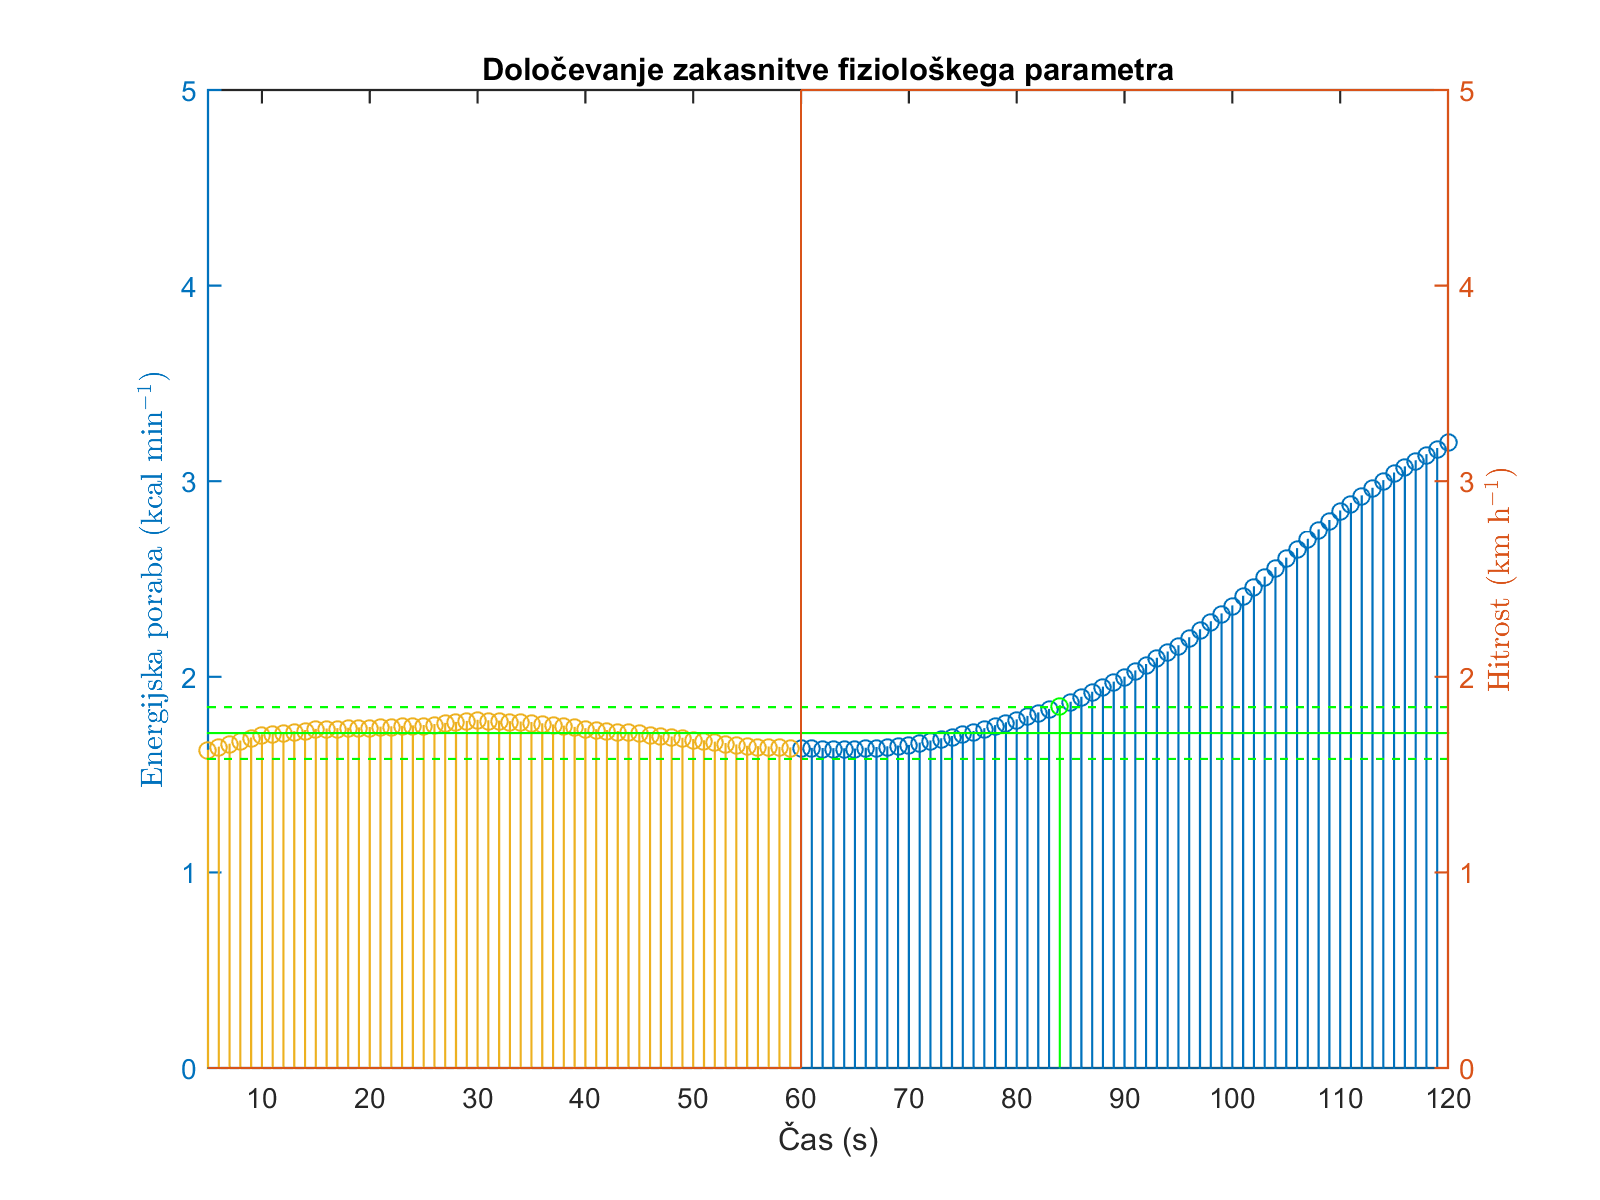
\includegraphics[width=\columnwidth]{./Slike/lag-estimation-1-eem.png}
		\caption{Zakasnitev za subjekt 1.}
		\label{fig:lag-estimation-1-eem}
	\end{subfigure}
	~
	\begin{subfigure}[t]{0.45\columnwidth}
		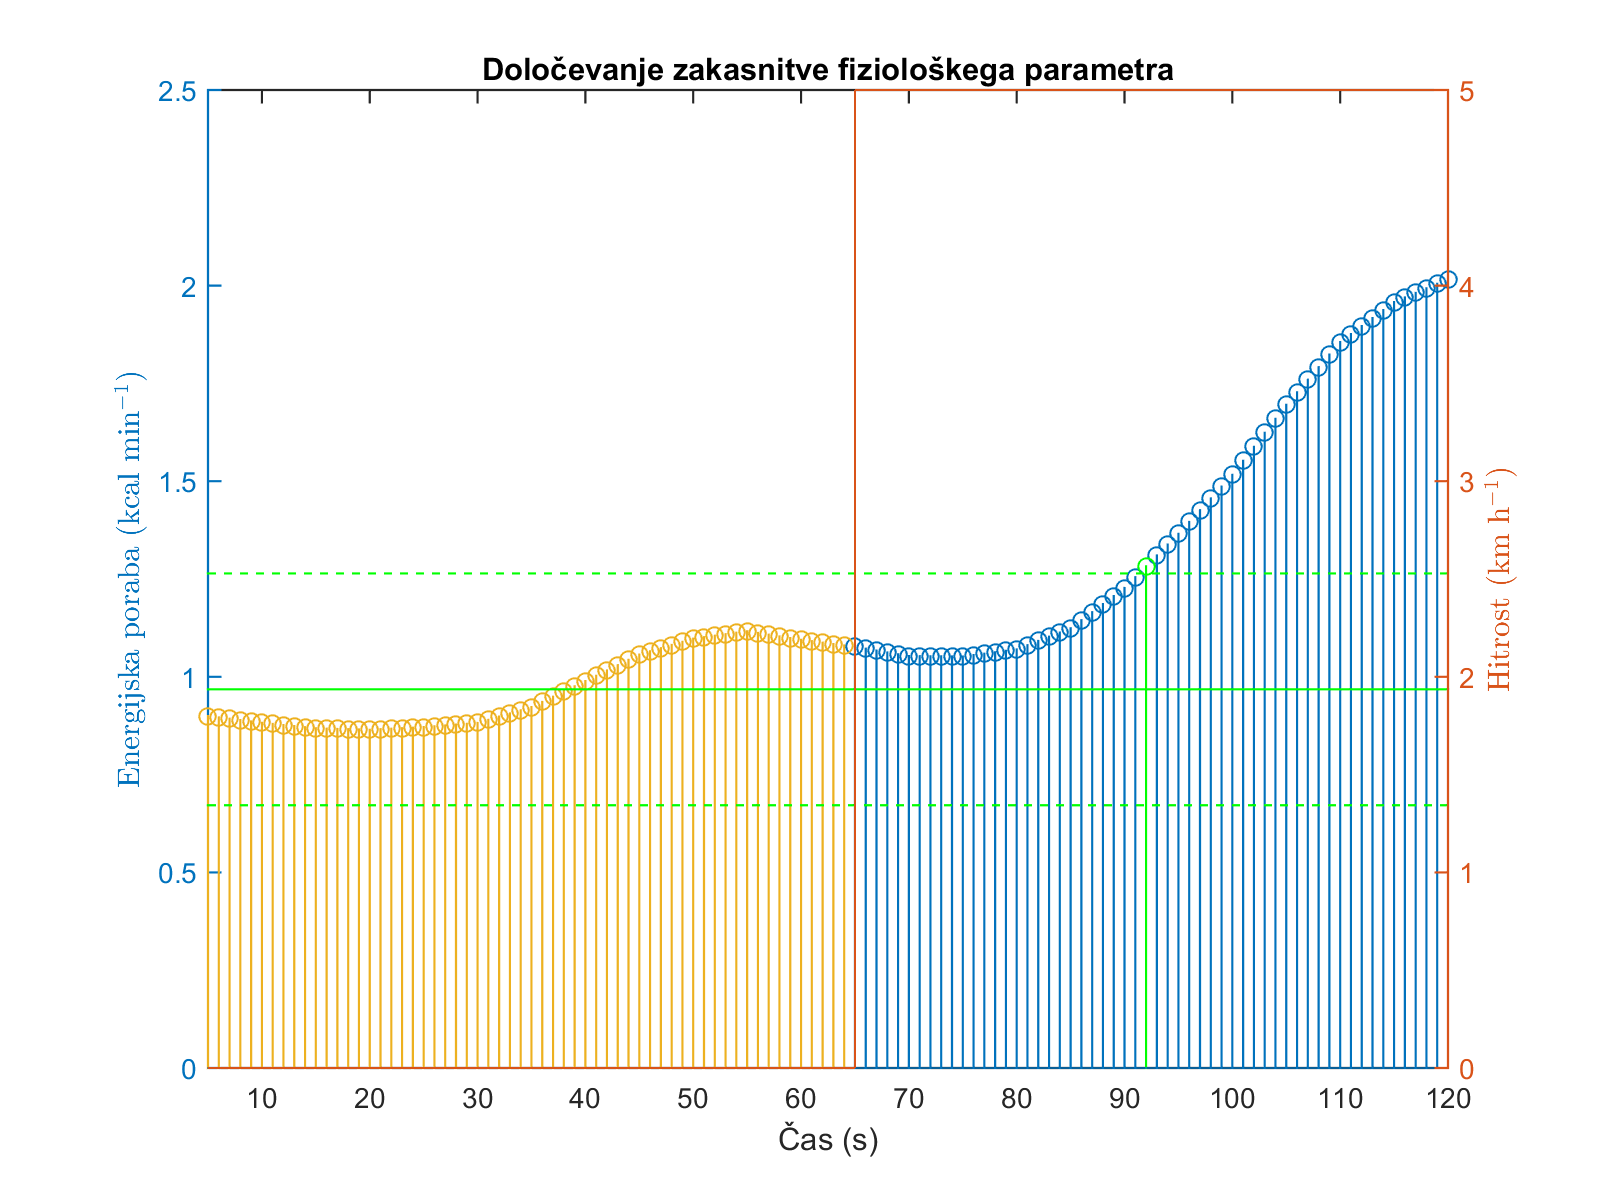
\includegraphics[width=\columnwidth]{./Slike/lag-estimation-2-eem.png}
		\caption{Zakasnitev za subjekt 2.}
		\label{fig:lag-estimation-2-eem}
	\end{subfigure}
	~
	\begin{subfigure}[t]{0.45\columnwidth}
		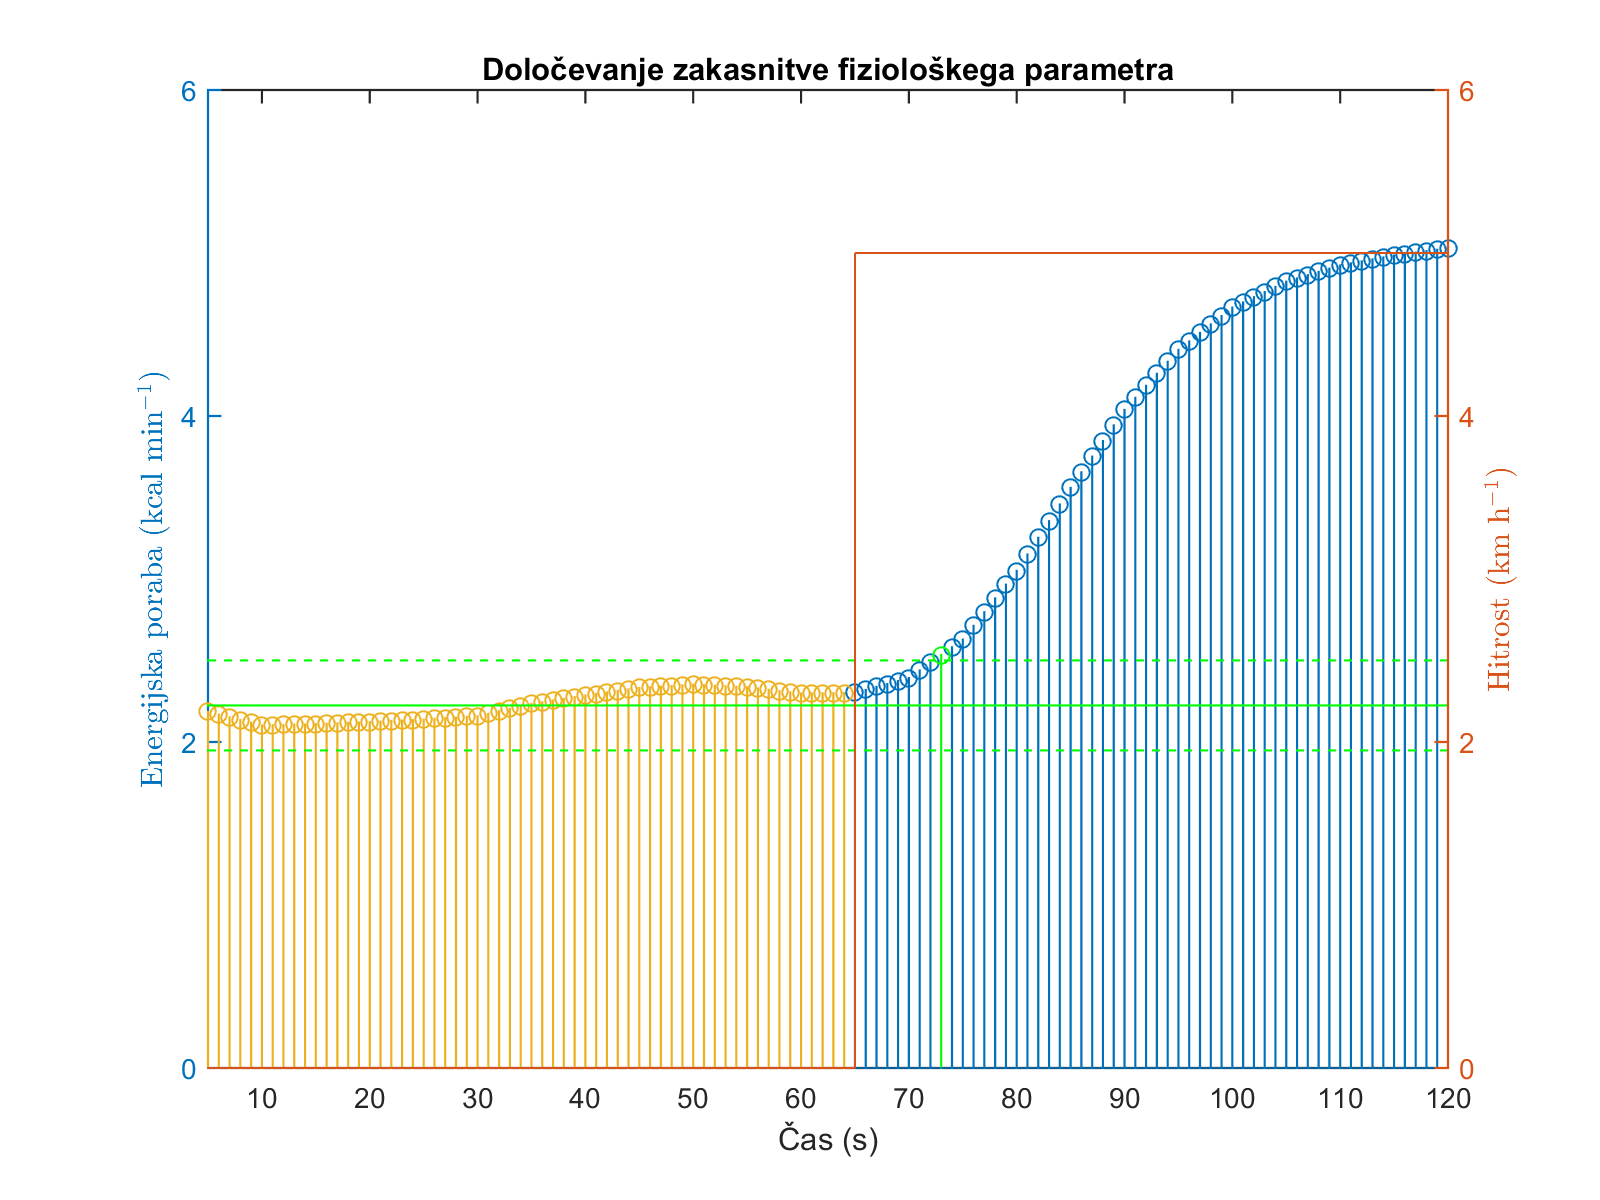
\includegraphics[width=\columnwidth]{./Slike/lag-estimation-3-eem.png}
		\caption{Zakasnitev za subjekt 3.}
		\label{fig:lag-estimation-3-eem}
	\end{subfigure}
	~
	\begin{subfigure}[t]{0.45\columnwidth}
		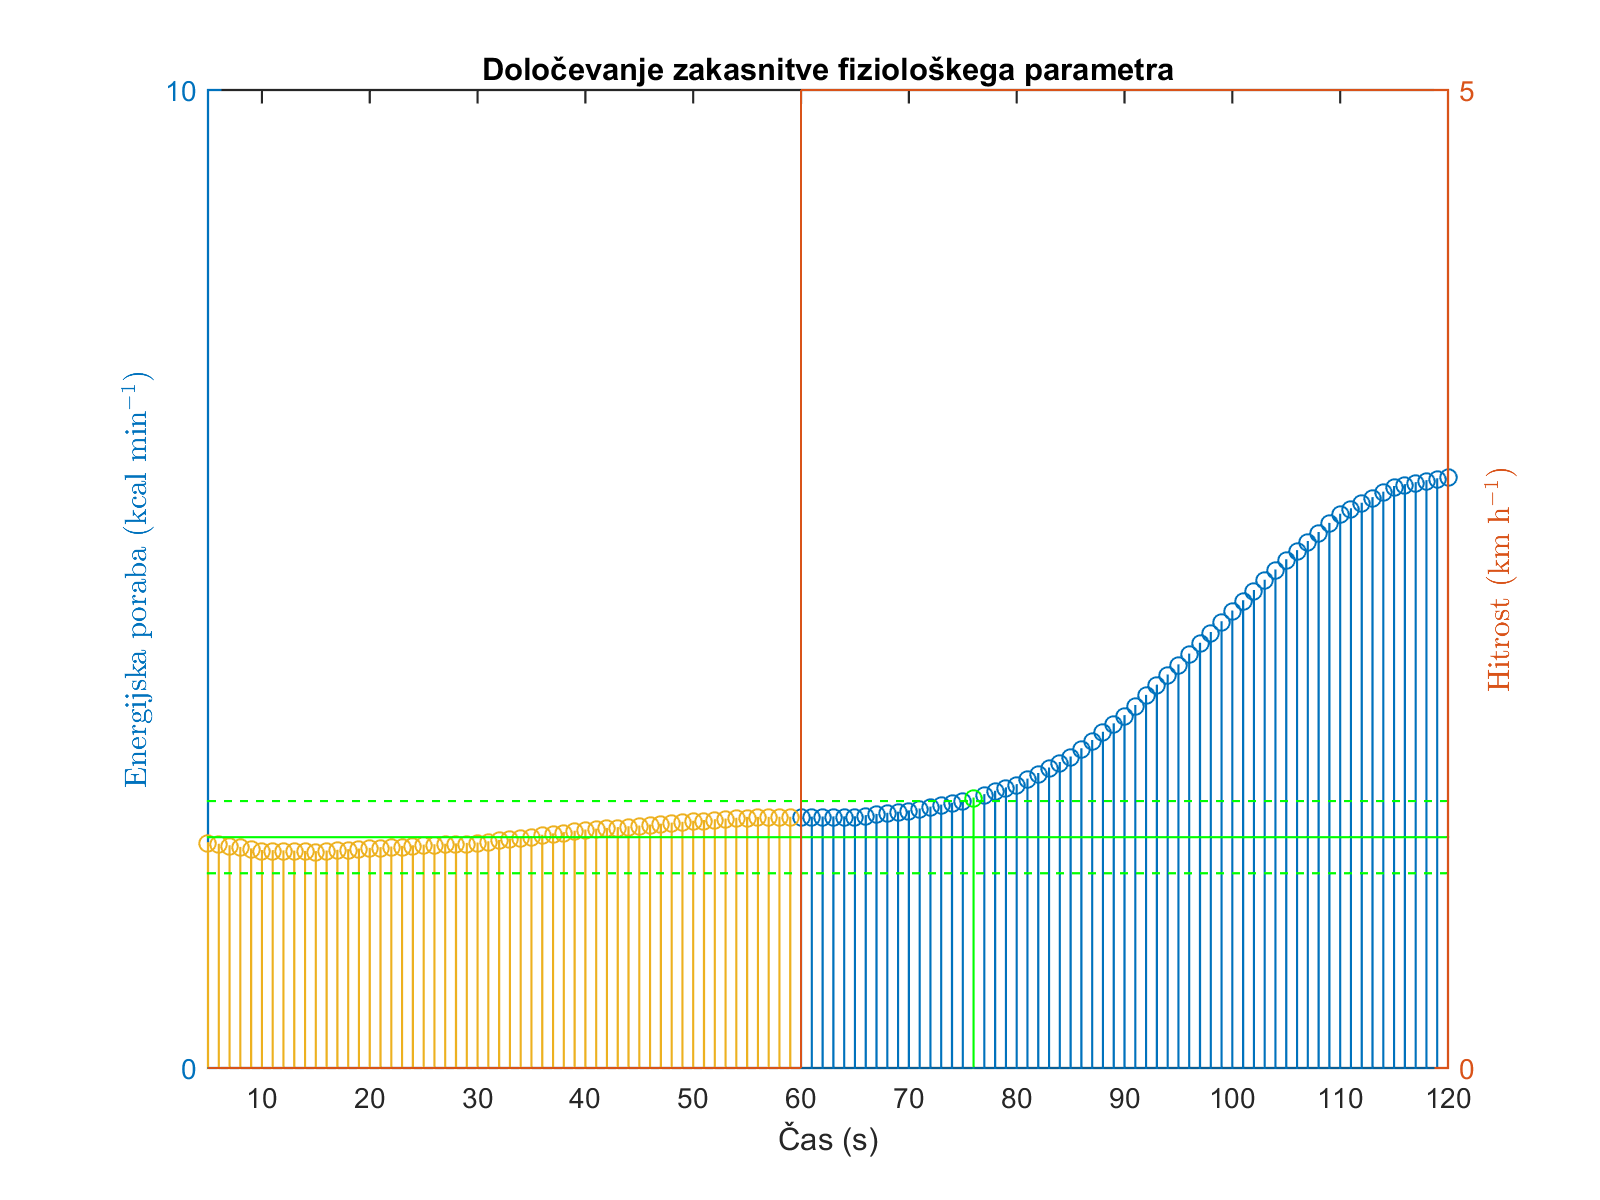
\includegraphics[width=\columnwidth]{./Slike/lag-estimation-4-eem.png}
		\caption{Zakasnitev za subjekt 4.}
		\label{fig:lag-estimation-4-eem}
	\end{subfigure}
	~
	\begin{subfigure}[t]{0.45\columnwidth}
		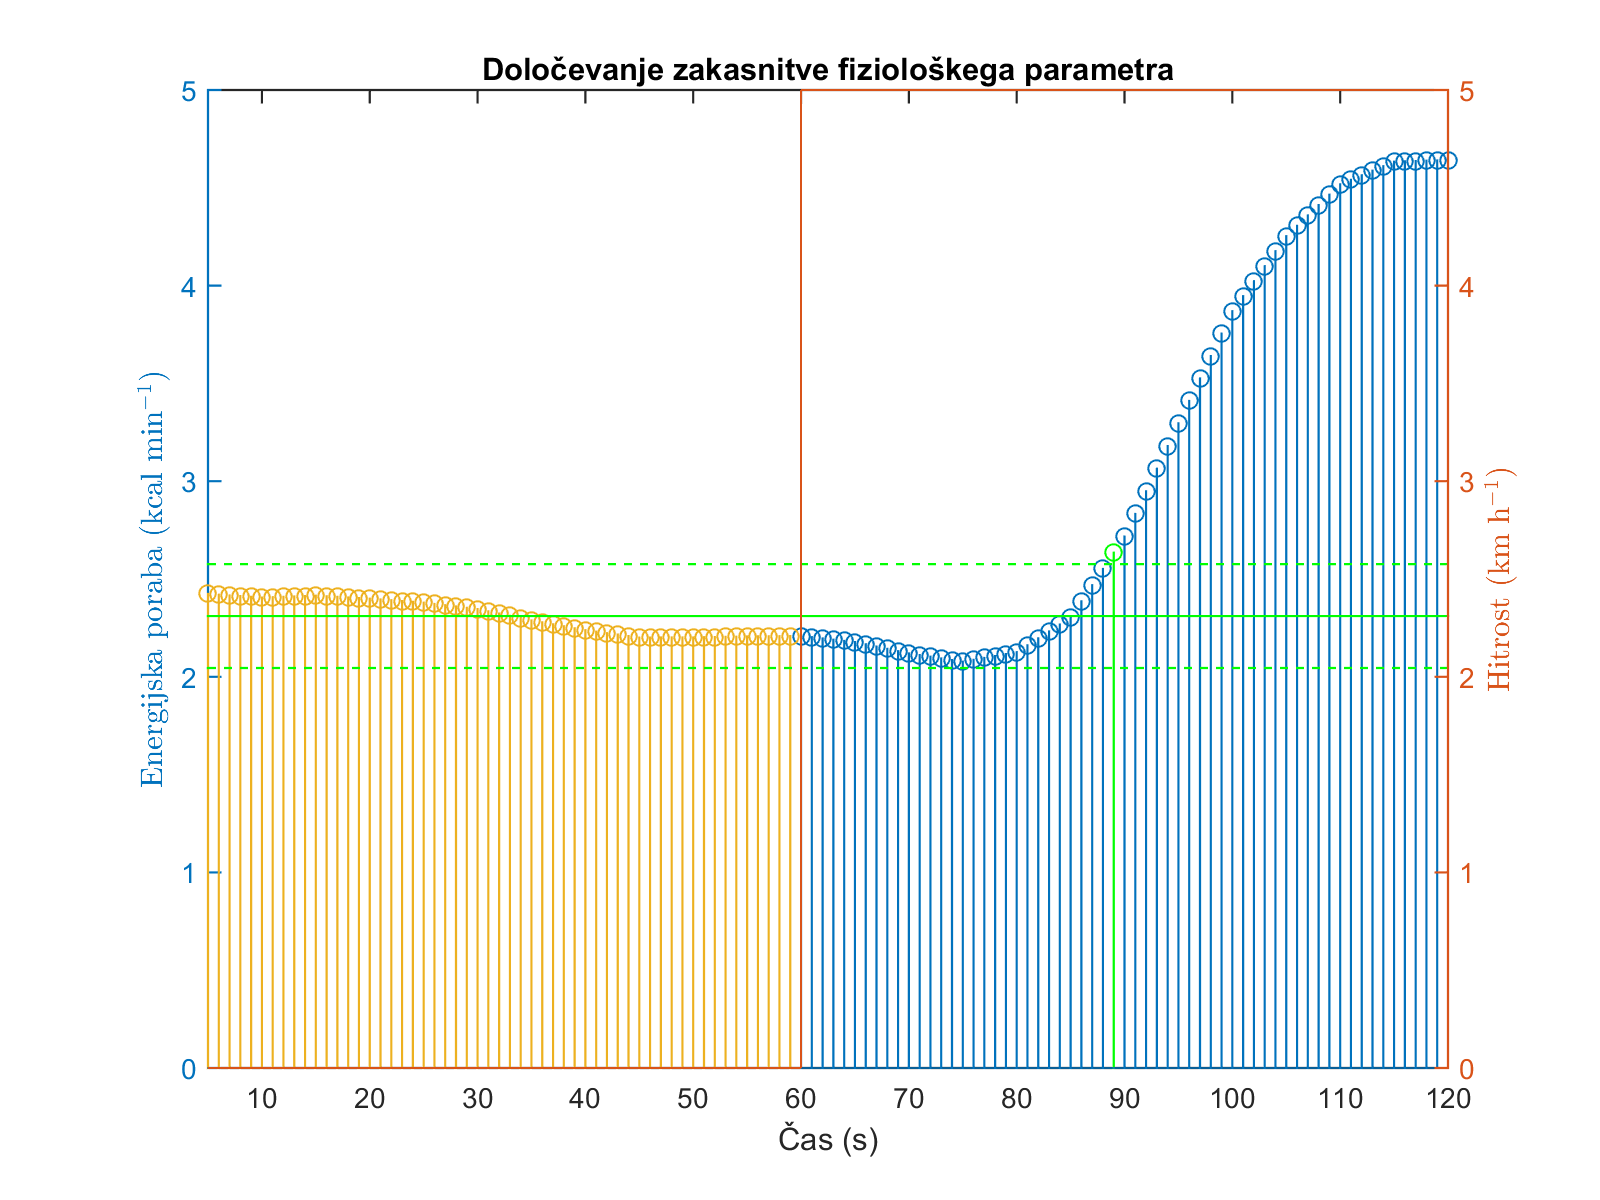
\includegraphics[width=\columnwidth]{./Slike/lag-estimation-5-eem.png}
		\caption{Zakasnitev za subjekt 5.}
		\label{fig:lag-estimation-5-eem}
	\end{subfigure}
	~
	\begin{subfigure}[t]{0.45\columnwidth}
		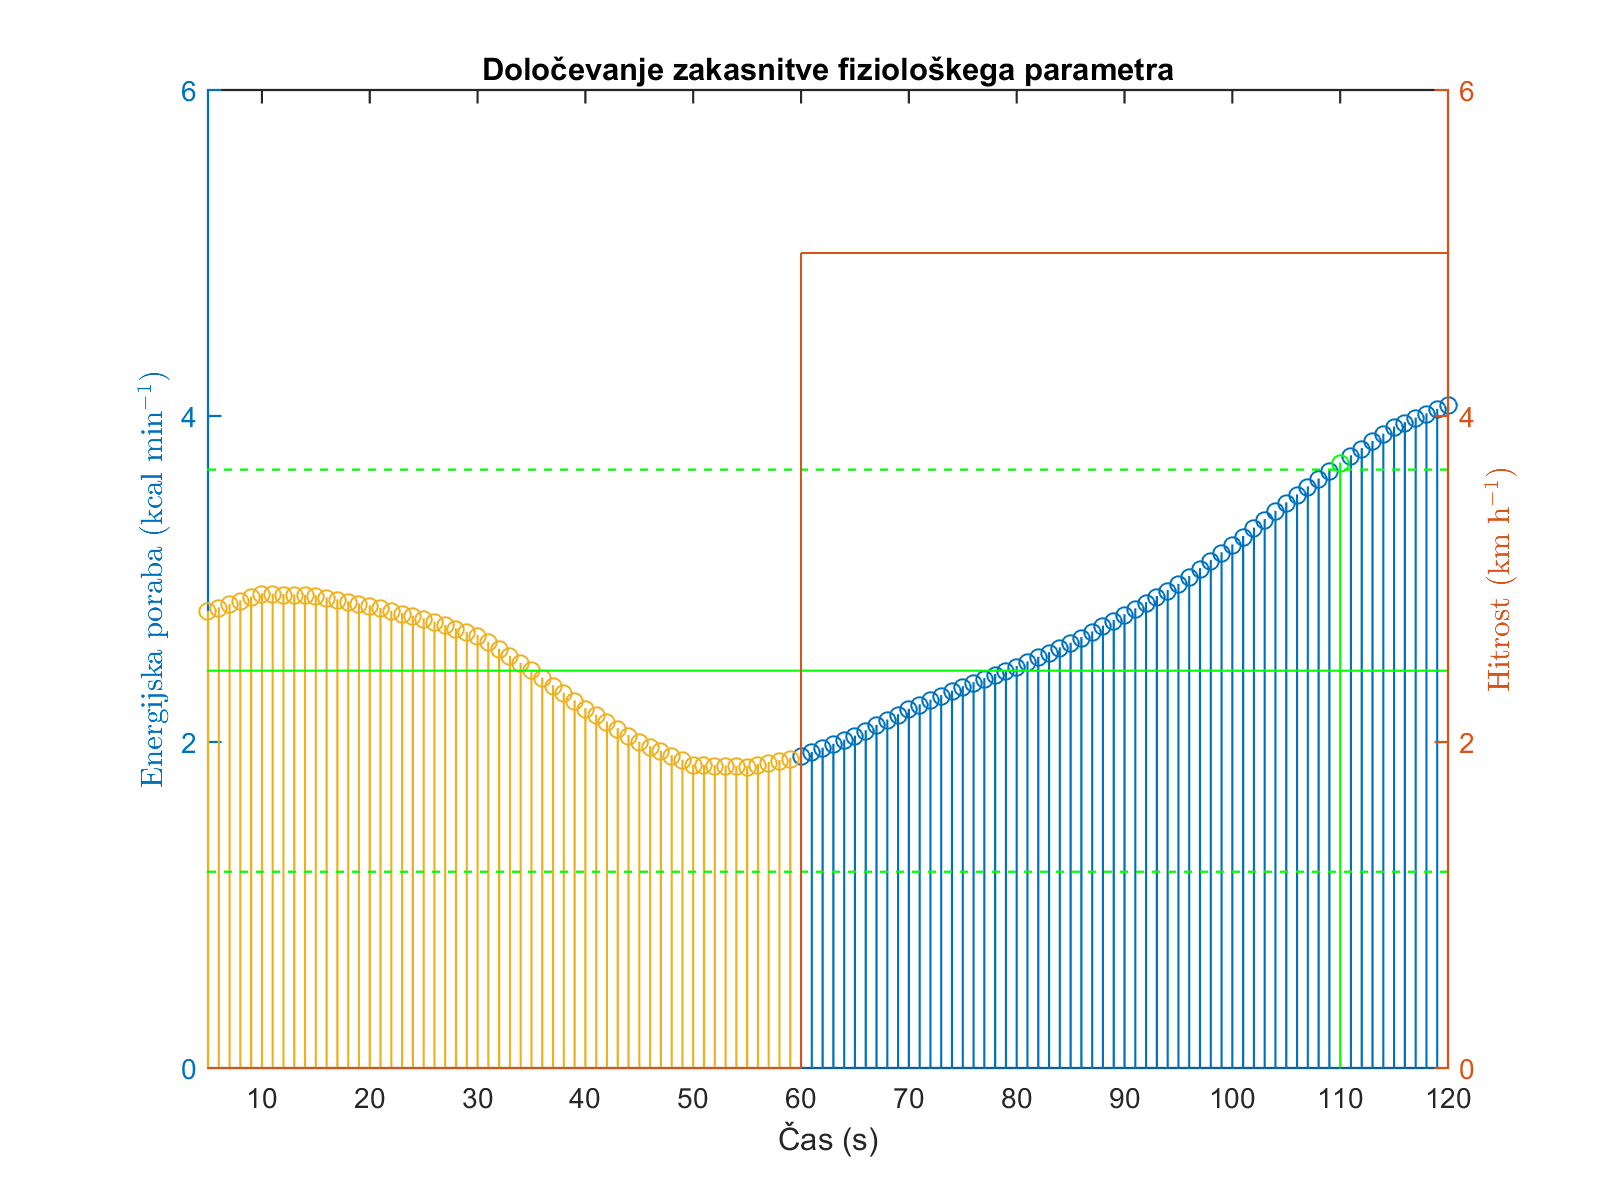
\includegraphics[width=\columnwidth]{./Slike/lag-estimation-6-eem.png}
		\caption{Zakasnitev za subjekt 6.}
		\label{fig:lag-estimation-6-eem}
	\end{subfigure}
	\caption{}
	\label{fig:lag-estimation-stage2}
\end{figure}










\subsection{Terenski eksperimenti}
Pri terenskih eksperimentih smo postopek z optičnim tokom in postopek s prostorskim tokom preverili še v realističnem okolju. Šest igralcev je igralo squash igro z dvema setoma. Tako smo pridobili podatke za 3 igre, ki so trajale \SI{16}{min} \SI{14}{min} in \SI{11}{min}. Postopki procesiranja in protokoli procesiranja so enaki kot v laboratorijskih eksperimentih 2. faze. 

\begin{figure}[htb]
	\centering
	\begin{subfigure}{0.45\columnwidth}
		%\includegraphics[width=\columnwidth]{./Slike/normal-sv-150.png}
		\caption{stranska slika}
	\end{subfigure}
	~
	\begin{subfigure}{0.45\columnwidth}
		%\includegraphics[width=\columnwidth]{./Slike/normal-bv-150.png}
		\caption{hrbtna slika}
	\end{subfigure}
	\caption{Hrbtna in stranska 150. slika RGB posnetkov iz prve serije.}
	\label{fig:primer-posnetka-teren}
\end{figure}

\paragraph{Pridobivanje podatkov.}
Igrišče smo snemali z dvema Microsoft Xbox Kinect V2 kamerama, ki sta bili oddaljeni ena od druge za približno \SI{2}{m}. Vsaka kamera je pokrivala svojo polovico igrišča. Razdalja od tal je znašala približno \SI{3}{m}. Kameri sta bili tako pozicionirani nad zaščitnim steklom. S tem nismo dobili odbojev laserskih žarkov, ki so namenjeni za pridobivanje globinske slike. Kot $\theta$ (rotacija okoli x osi) je bil približno $30\stopinj$ tako, da so kamere pokrivale prvo polovico igrišča do linije serviranja.

Pridobili smo barvne RGB in globinske DEPTH slike. Snemali smo v ločljivosti $512 \times 424$. Hitrost posnetkov je znašala \SI{30}{fps}. Kameri smo časovno sinhronizirali po NTP protokolu.

Fiziološke parametre smo pridobili s pomočjo prenosnega sistema za direktno ergospirometrijo tipa ``breath  by breath'' Cosmed K4B2. Frekvenca vzorčenja se je spreminjala, v povrečju pa je znašala \SI{0.5}{\hertz}. S testom smo pridobili podatke energijske porabe šestih različnih merjencev z oznakammi: SUBJ1, SUBJ2, SUBJ7, SUBJ8, SUBJ9 in SUBJ10.

\paragraph{Protokol izvajanja meritev.}
Posamezno igro smo pričeli s 5 minutnim ogrevalnim tekom. Sledilo je igranje na dva seta do 10 dobljenih točk z upoštevanjem dveh točk razlike. Med setoma so igralci počivali 2 minute. Ogrevanja in počivanja s kamerami nismo merili. Seta posamezne igre smo združili v en posnetek.

\chapter{Rezultati}\label{sec:rezultati}
All energy consumption and heart rate models were validated on previously described test samples. For comparison between the different models we have chosen validation measures: correlation coefficient (CORR), relative absolute error (RAE) and root relative square error (RRSE) \cite{witten2005data}. We have also added ratio between number of support vectors and number of training data (nSV). The higher the value of the CORR the better, with RAE, RRSE and nSV is other way around.

Models were also evaluated with cross testing. This testing was done only by the type of input data (side-view or back-view). \textit{sv} models, that were made with learning samples from side-view camera were first tested with testing samples from side-view camera and then with back-view camera. Hereafter tests with input data from side-view camera are marked with \textit{sv} in brackets and tests with input data from back-view camera are marked with \textit{bv} in brackets.


















\section{Eksperimenti 1. faze}


\subsection{Preliminarni testi}

\subsubsection{Optimizacija HOOF deskriptorjev}\label{sec:rezultati-optimizacija-hoof}
Parameter $N_{HOOF}$ smo določili na podlagi rezultatov evaluacije v tabeli \ref{tab:nhoof} in grafov korelacije med referenčnimi podatki in predikcijo \ref{fig:corr-hoof}.

V tabeli \ref{tab:nhoof} lahko vidimo, da se povečevanjem števila stolpcev rezultati bistveno ne razlikujejo. Najbojlši rezultate nam sicer daje $120$ stolpcev, vendar pa smo za potrebe naše metode uporabili $N_{HOOF}=60$, ki je ravno tako dal zadovoljive rezultate. S takim številom smo zagotovili dobro delovanje glede na minimalno vrednost, še vseeno pa ne gre za tako veliko število, ko bi do izraza prišle amplitude šumnih vektorjev.

\begin{table}[!htbp]
	\centering
	\begin{tabular}{S[table-format=2.0] S[table-format=1.3] S[table-format=1.3] S[table-format=1.3] S[table-format=2.2]}
		\toprule
		\thead{$\mathbf{N_{HOOF}}$} & \thead{$\mathbf{r}$} & \thead{RAE} & \thead{RRSE} & \thead{nSV [\%]}\\
		\midrule%nSV
		30 & 0.978 & 0.296 & 0.304 & \boldentry{2}{2}{62.81}\\%18089
		\boldentry{2}{0}{60} & 0.980 & 0.277 & 0.289 & 81.21\\%23388
		120 & \boldentry{1}{2}{0.983} & \boldentry{1}{3}{0.261} & \boldentry{1}{3}{0.273} & 74.39\\%21424
		160 & 0.982 & 0.272 & 0.284 & 71.68\\%20644
		\bottomrule
	\end{tabular}
	\caption[Rezultati evaluacije modelov z različnim $N_{HOOF}$]{Rezultati evaluacije modelov z različnim številom stolpcev $N_{HOOF}$ HOOF deskriptorja. Optimalni rezultati so odebeljeni. Kljub dobrim rezultatom modela z $N_{HOOF}=120$ smo izbrali $N_{HOOF}=60$, ker nanj šum manj vpliva.}
	\label{tab:nhoof}
\end{table}

\begin{figure}[!htbp]
	\centering
	\begin{subfigure}[t]{0.45\columnwidth}
		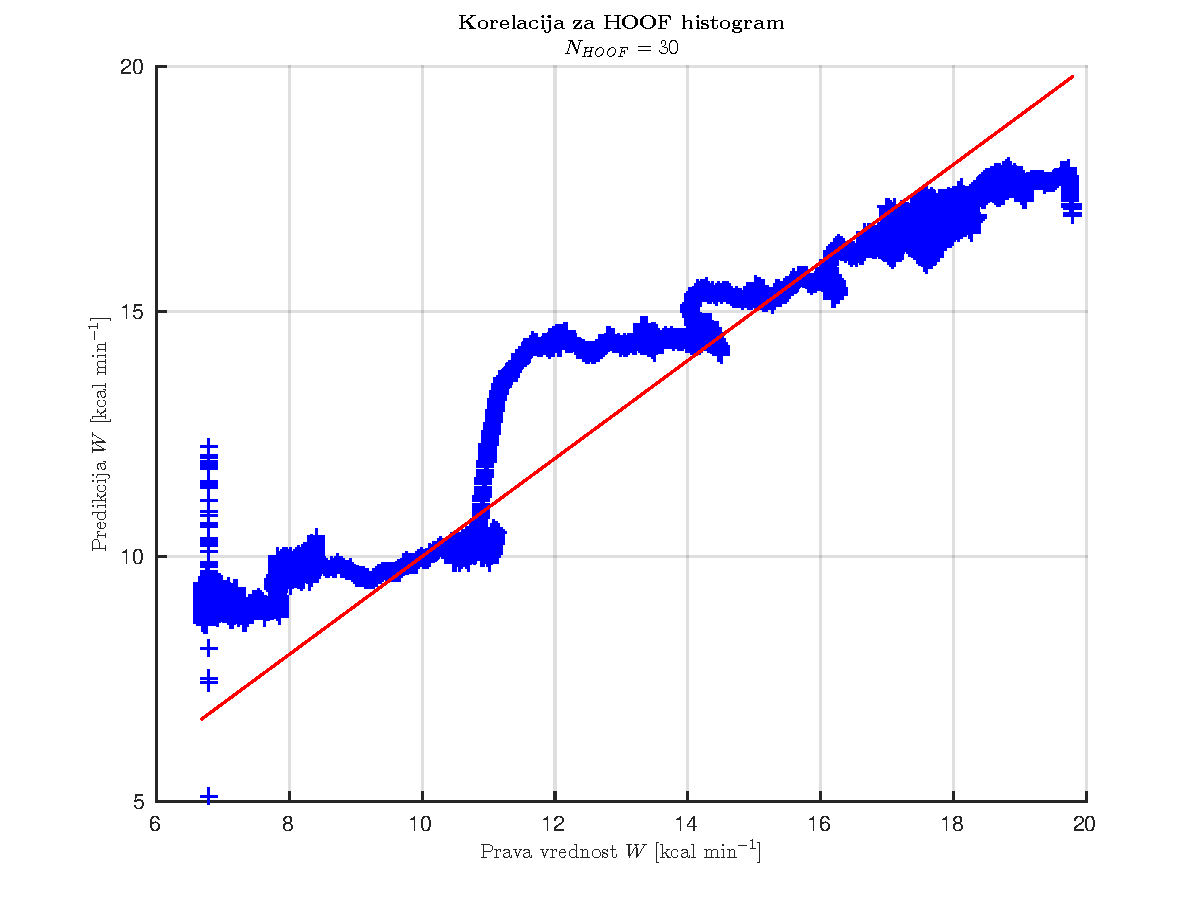
\includegraphics[width=\columnwidth]{corr-hoof-30-sl}
		\caption{Korelacija $N_{HOOF}=30$.}
		\label{fig:corr-hoof-30}
	\end{subfigure}
	~
	\begin{subfigure}[t]{0.45\columnwidth}
		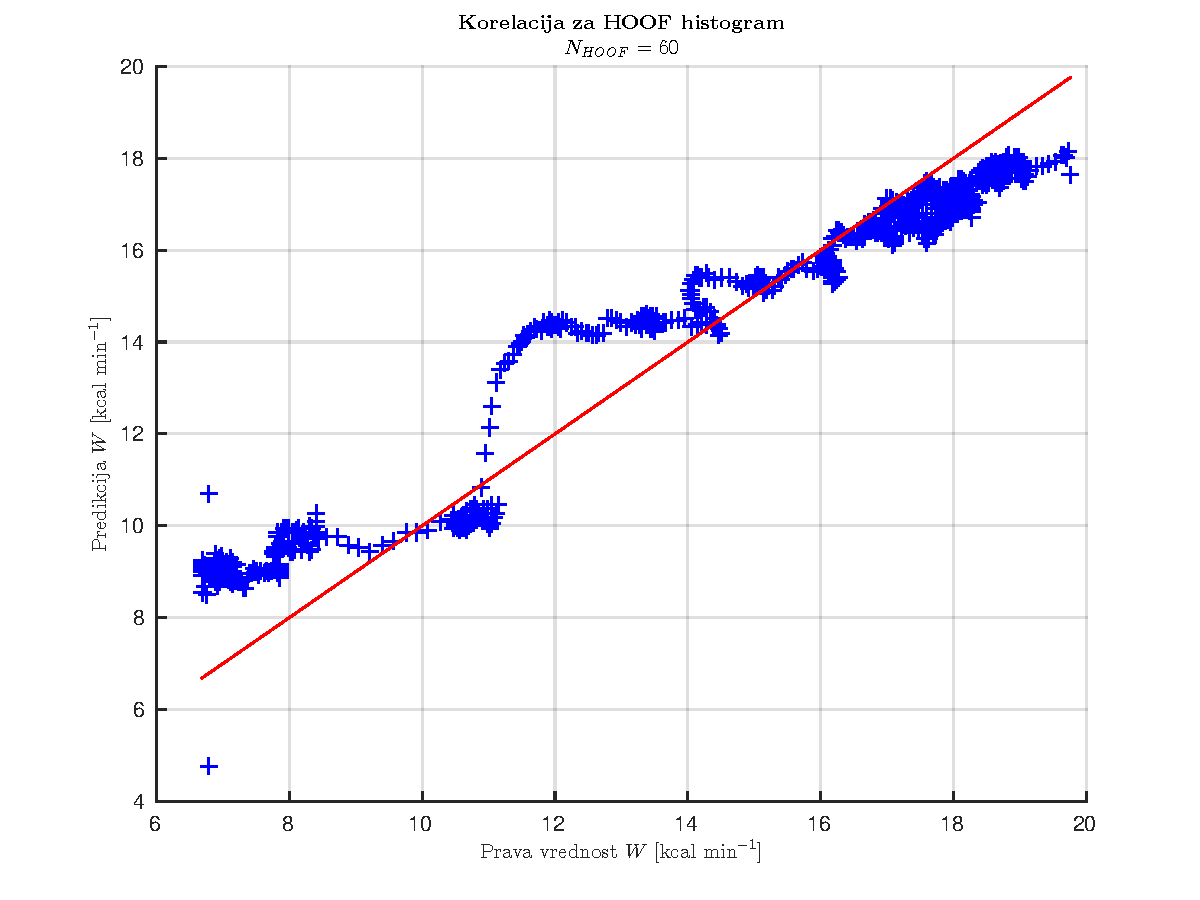
\includegraphics[width=\columnwidth]{corr-hoof-60-sl}
		\caption{Korelacija $N_{HOOF}=60$.}
		\label{fig:corr-hoof-60}
	\end{subfigure}
	~
	\begin{subfigure}[b]{0.45\columnwidth}
		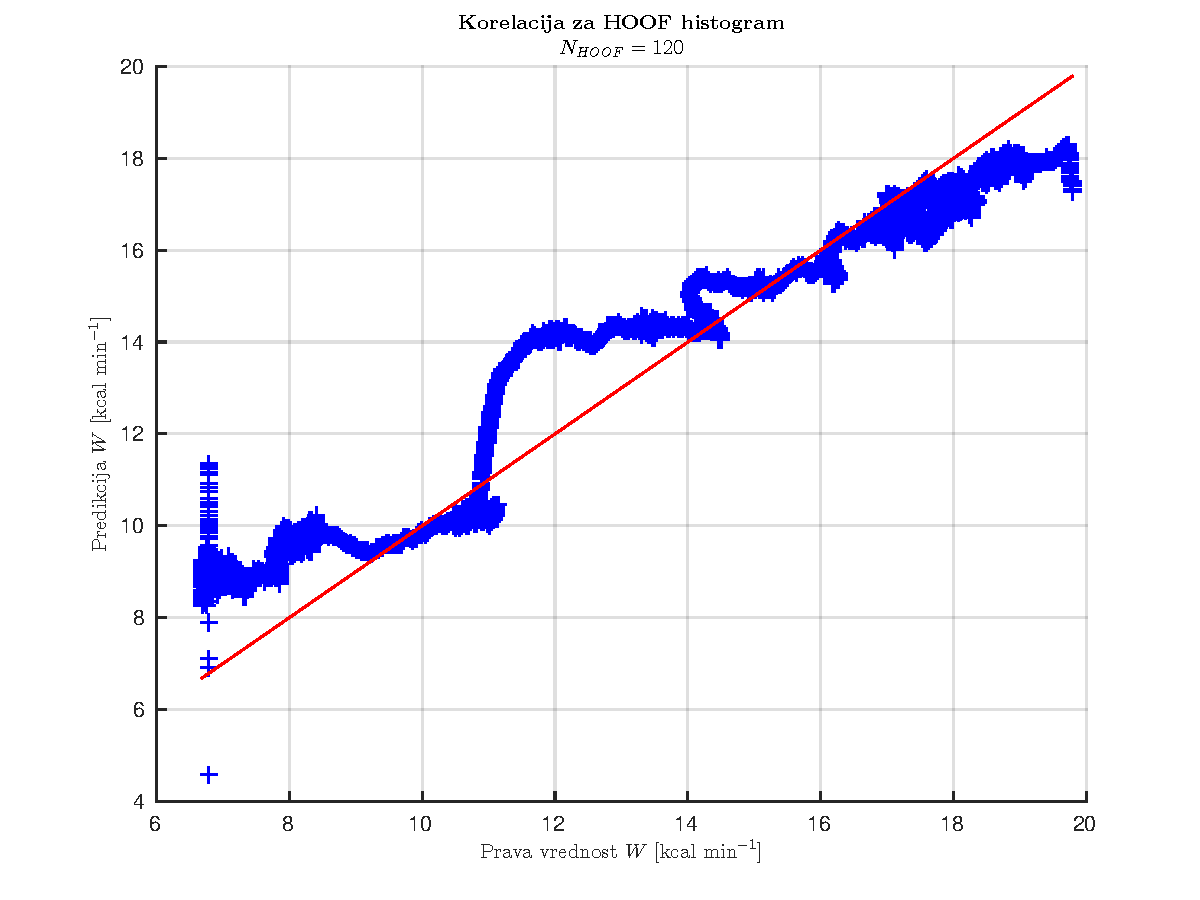
\includegraphics[width=\columnwidth]{corr-hoof-120-sl}
		\caption{Korelacija $N_{HOOF}=120$.}
		\label{fig:corr-hoof-120}
	\end{subfigure}
	~
	\begin{subfigure}[b]{0.45\columnwidth}
		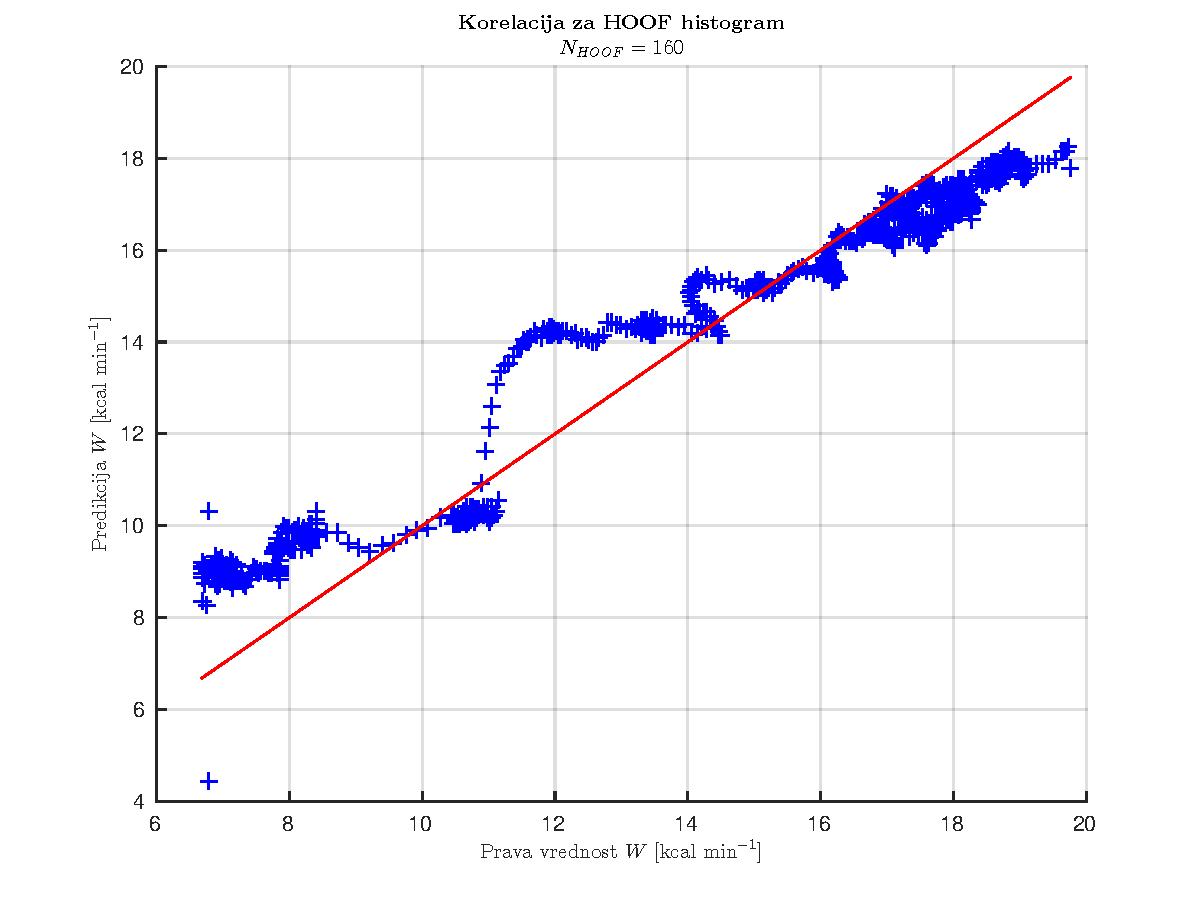
\includegraphics[width=\columnwidth]{corr-hoof-160-sl}
		\caption{Korelacija $N_{HOOF}=160$.}
		\label{fig:corr-hoof-160}
	\end{subfigure}
	\caption[Grafi korelacij modelov z različnim $N_{HOOF}$]{Grafi korelacij modelov z različnim številom stolpcev $N_{HOOF}$ HOOF deskriptorja. Rezultati so si zelo podobni.}
	\label{fig:corr-hoof}
\end{figure}












\subsubsection{Optimizacija HAFA deskriptorjev}\label{sec:rezultati-optimizacija-hafa}
Parameter $N_{HAFA}$ smo določili na podlagi rezultatov evaluacije v tabeli \ref{tab:nhafa} in grafov korelacije med referenčnimi podatki in predikcijo \ref{fig:corr-hafa}.

\begin{table}[!htbp]
	\centering
	\begin{tabular}{S[table-format=2.0] S[table-format=1.3] S[table-format=1.3] S[table-format=1.3] S[table-format=2.2]}
		\toprule
		\thead{$\mathbf{N_{HAFA}}$} & \thead{$\mathbf{r}$} & \thead{RAE} & \thead{RRSE} & \thead{nSV [\%]}\\
		\midrule%nSV
		30 & 0.984 & 0.213 & 0.231 & 62.08 \\%17879/28799
		\boldentry{2}{0}{60} & \boldentry{1}{3}{0.984} & \boldentry{1}{3}{0.211} & \boldentry{1}{3}{0.228} & \boldentry{2}{2}{62.60} \\%18028
		120 & 0.984 & 0.211 & 0.228 & 62.63 \\%18037
		160 & 0.984 & 0.211 & 0.228 & 62.63 \\%18037
		\bottomrule
	\end{tabular}
	\caption[Rezultati evaluacije modelov z različnim $N_{HAFA}$]{Rezultati evaluacije modelov z različnim številom stolpcev $N_{HAFA}$ HAFA deskriptorja. Optimalni rezultati so odebeljeni.}
	\label{tab:nhafa}
\end{table}

V tabeli \ref{tab:nhafa} lahko vidimo, da so rezultati praktično enaki. Za našo metodo smo izbrali $N_{HAFA}=60$, kar v grobem predstavlja $60$ različnih hitrosti z maksimalno amplitudo \SI{60}{px.f^{-1}}.

\begin{figure}[!htbp]
	\centering
	\begin{subfigure}[t]{0.45\columnwidth}
		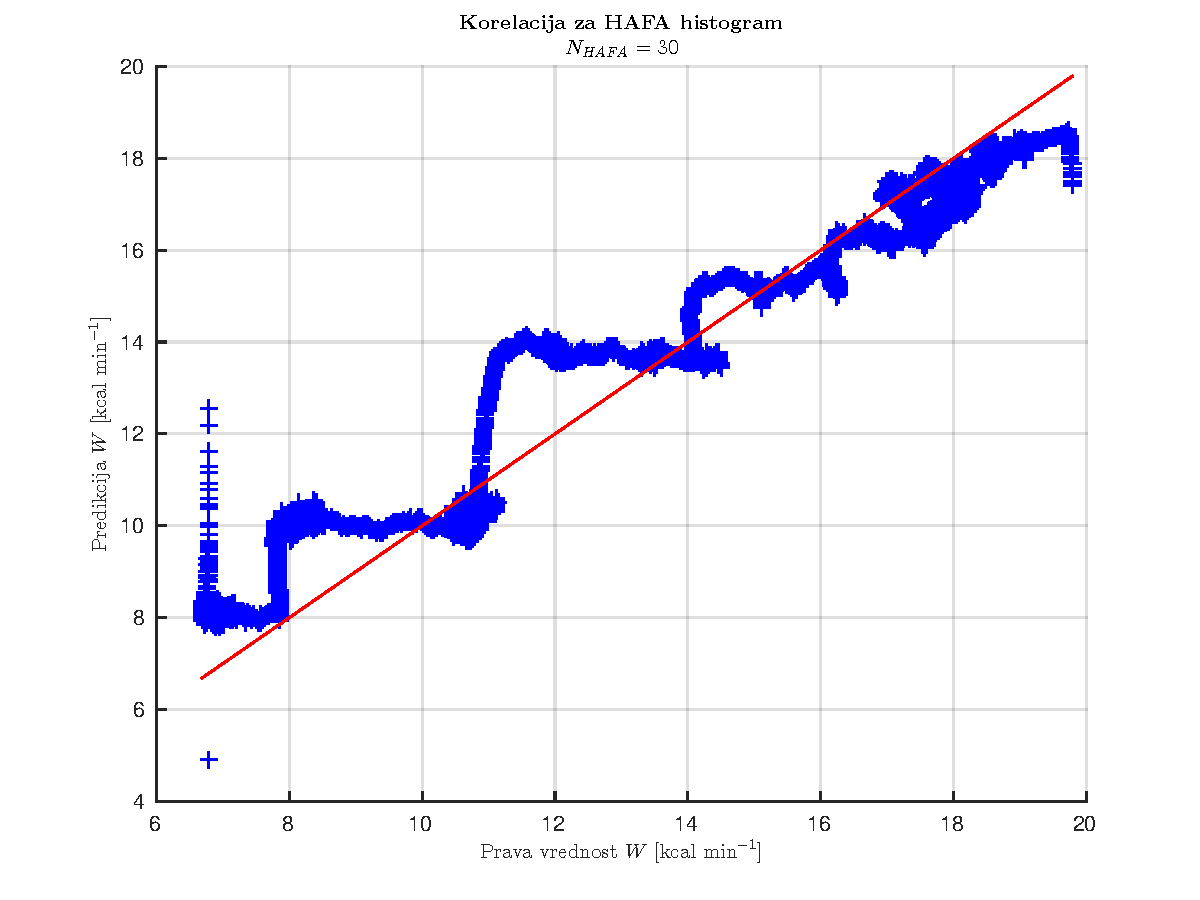
\includegraphics[width=\columnwidth]{corr-hafa-30-sl}
		\caption{Korelacija $N_{HAFA}=30$.}
		\label{fig:corr-hafa-30}
	\end{subfigure}
	~
	\begin{subfigure}[t]{0.45\columnwidth}
		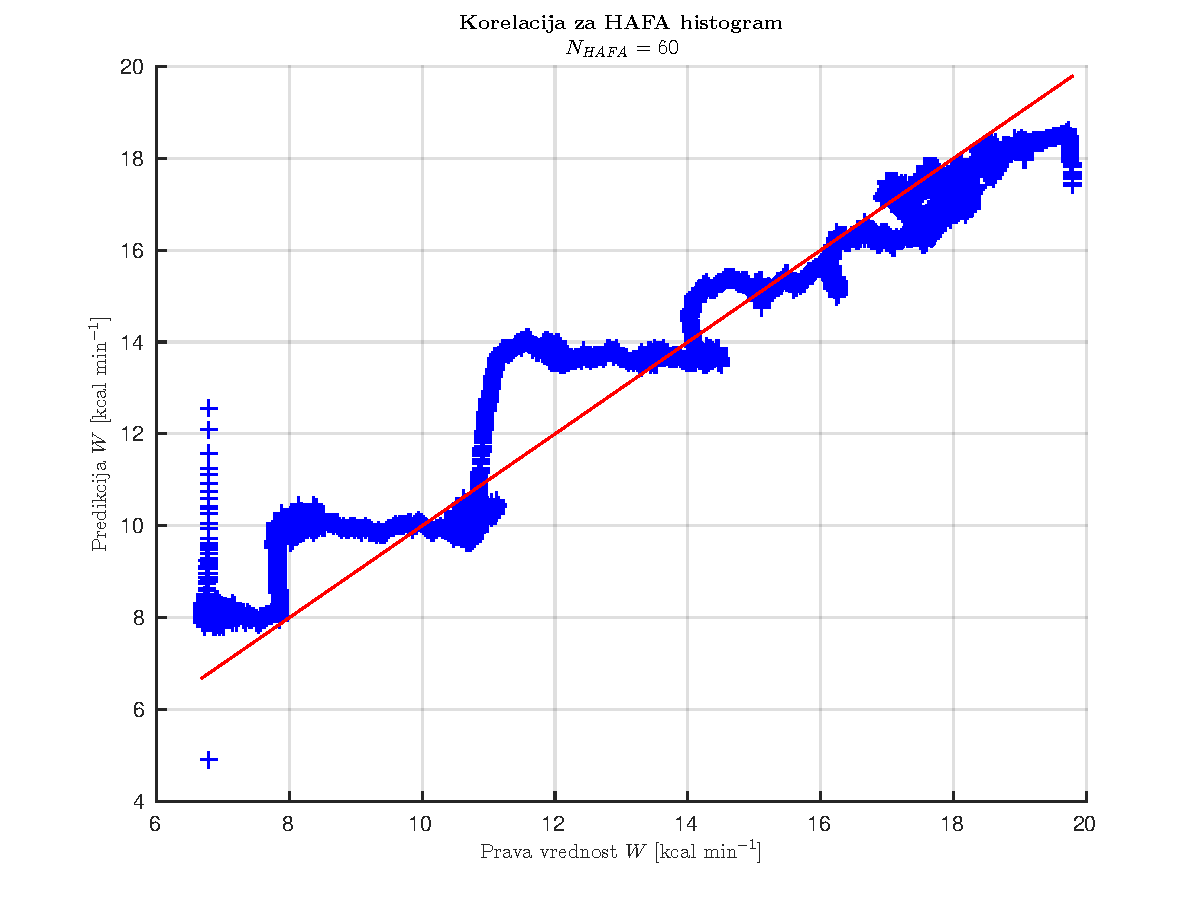
\includegraphics[width=\columnwidth]{corr-hafa-60-sl}
		\caption{Korelacija $N_{HAFA}=60$.}
		\label{fig:corr-hafa-60}
	\end{subfigure}
	~
	\begin{subfigure}[b]{0.45\columnwidth}
		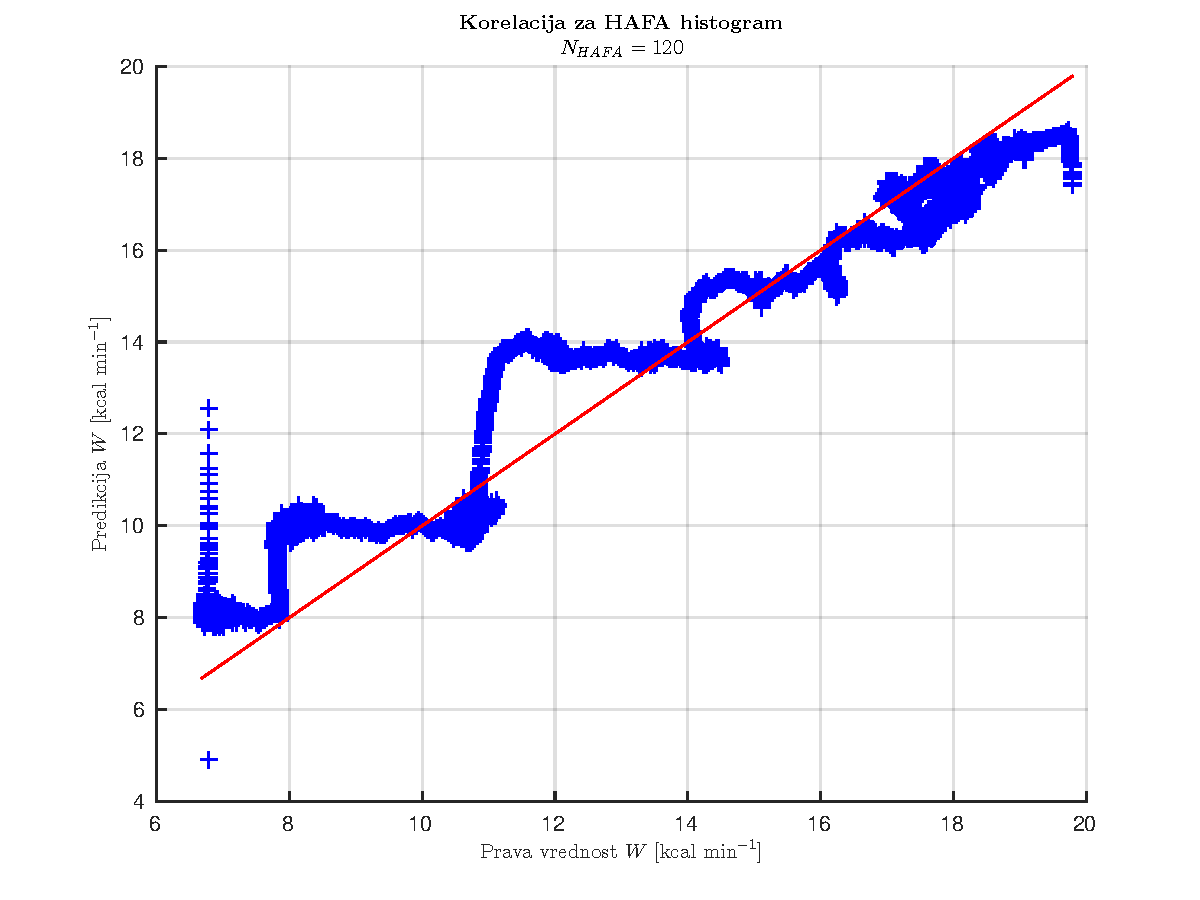
\includegraphics[width=\columnwidth]{corr-hafa-120-sl}
		\caption{Korelacija $N_{HAFA}=120$.}
		\label{fig:corr-hafa-120}
	\end{subfigure}
	~
	\begin{subfigure}[b]{0.45\columnwidth}
		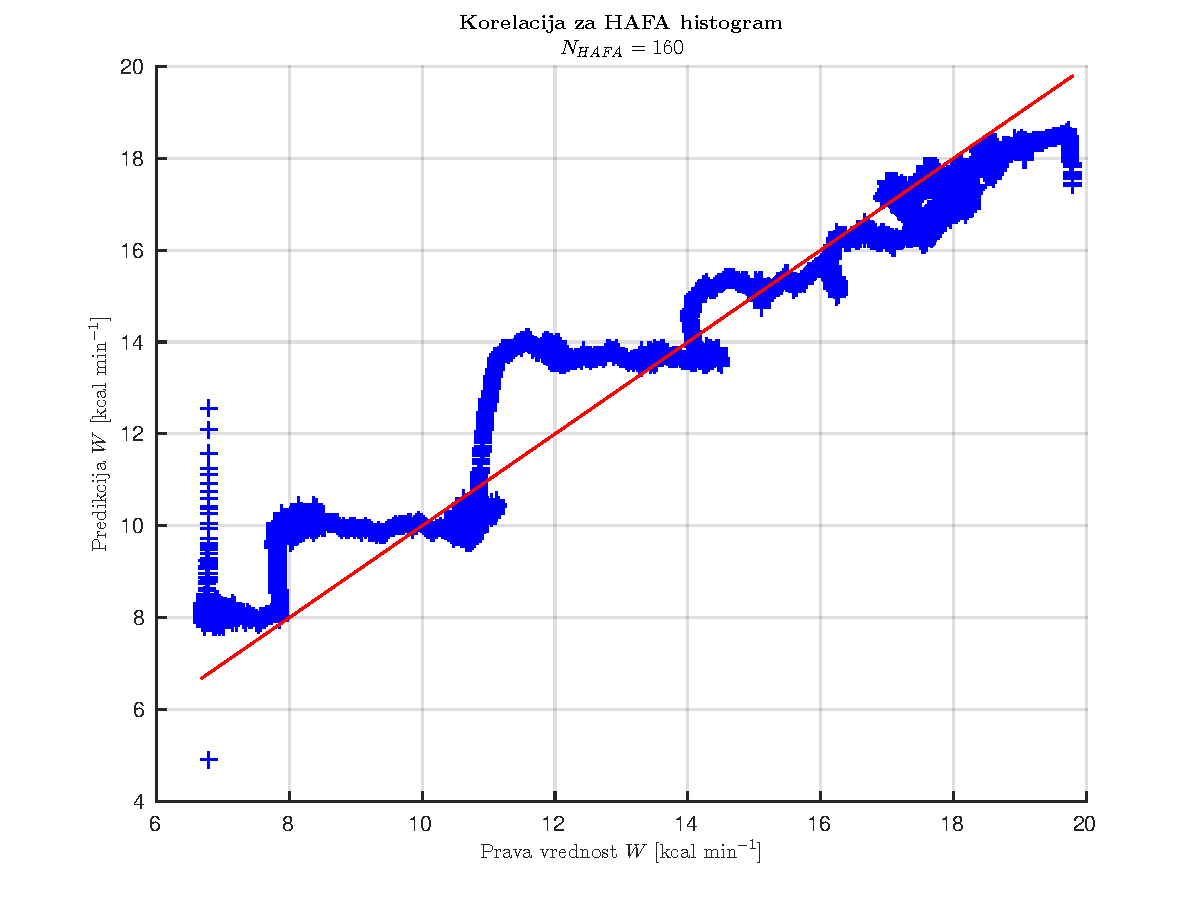
\includegraphics[width=\columnwidth]{corr-hafa-160-sl}
		\caption{Korelacija $N_{HAFA}=160$.}
		\label{fig:corr-hafa-160}
	\end{subfigure}
	\caption[Grafi korelacij modelov z različnim $N_{HAFA}$]{Grafi korelacij modelov z različnim številom stolpcev $N_{HAFA}$ HAFA deskriptorja. Rezultati so si zelo podobni.}
	\label{fig:corr-hafa}
\end{figure}











\subsubsection{Razširitev HOOF deskriptorja}\label{sec:rezultati-razsiritev-hoof}

\begin{table}[!htbp]
	\centering
	\begin{tabular}{l S[table-format=1.3] S[table-format=1.3] S[table-format=1.3] S[table-format=2.2]}
		\toprule
		\textbf{Deskriptor} & \thead{$\mathbf{r}$} & \thead{RAE} & \thead{RRSE} & \thead{nSV [\%]}\\
		\midrule%nSV
		HOOF & 0.992 & 0.336 & 0.317 & \boldentry{2}{2}{82.34} \\%2187/2656
		\textbf{HOOF-HAFA} & \boldentry{1}{3}{0.991} & \boldentry{1}{3}{0.157} & \boldentry{1}{3}{0.205} & 89.53 \\%2378
		\bottomrule
	\end{tabular}
	\caption[Rezultati evaluacije modelov z različnim deskriptorjem]{Rezultati evaluacije modelov z različnim deskriptorjem. Optimalni rezultati so odebeljeni. Vidimo lahko, da se bolje odnese razširjeni deskriptor HOOF-HAFA, čeprav model uporablja več podpornih vektorjev. }
	\label{tab:izbira}
\end{table}



\begin{figure}[!htbp]
	\centering
	\begin{subfigure}[t]{0.45\columnwidth}
		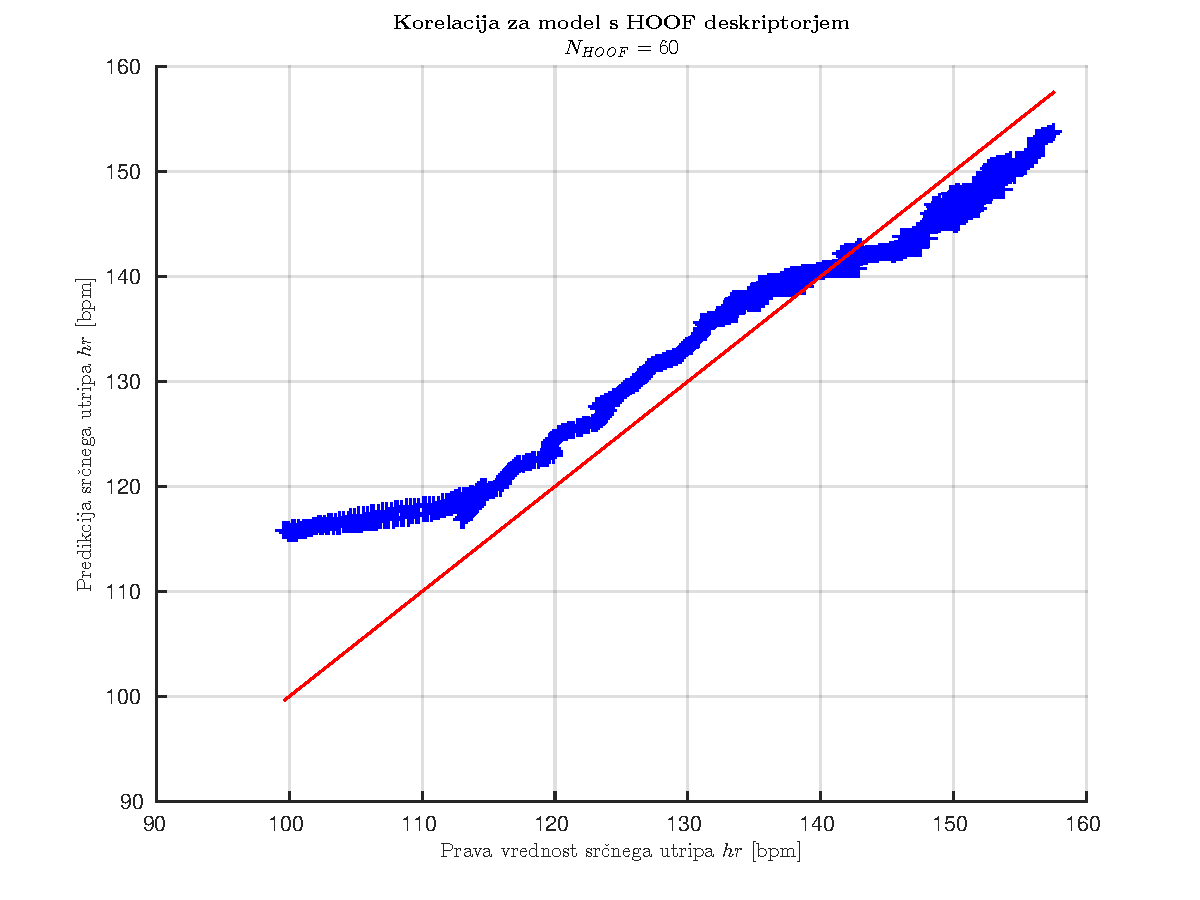
\includegraphics[width=\columnwidth]{corr-hoof-sl}
		\caption{Korelacija $N_{HOOF}=60$.}
		\label{fig:izbira-hoof}
	\end{subfigure}
	~
	\begin{subfigure}[t]{0.45\columnwidth}
		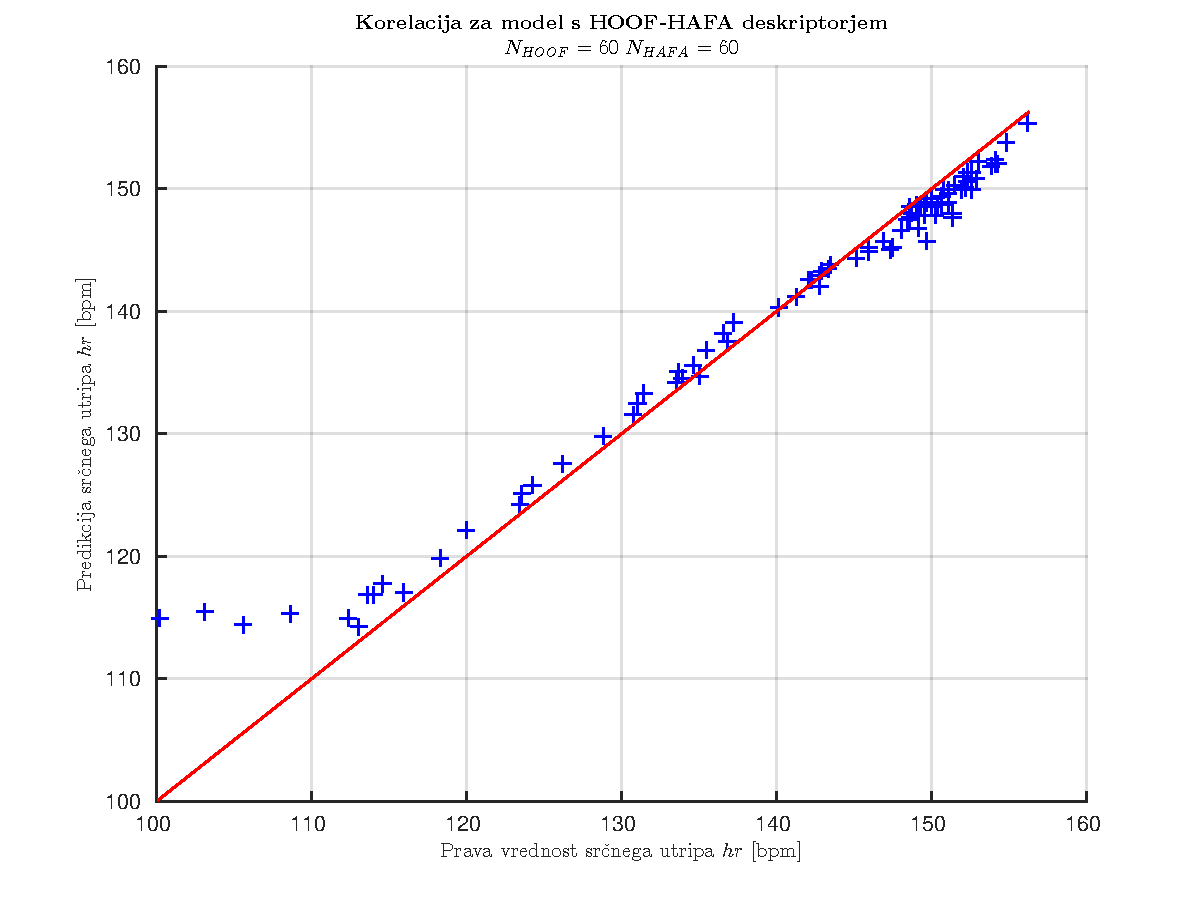
\includegraphics[width=\columnwidth]{corr-hoof-hafa-sl}
		\caption{Korelacija $N_{HOOF}=60$,\\$N_{HAFA}=60$.}
		\label{fig:izbira-hoofhafa}
	\end{subfigure}
	\caption[Primerjava modelov s HOOF in HOOF-HAFA deskriptorji]{Primerjava grafov korelacij modelov z različnimi deskriptorji. Model \subref{fig:izbira-hoof}) smo naučili s HOOF deskriptorjem. Model \subref{fig:izbira-hoofhafa}) smo naučili s HOOF in HAFA deskriptorjem. Posamezen vzorec je tako vseboval $120$ značilk. Pri primerjavi korelacije lahko opazimo vidno razliko. Model \subref{fig:izbira-hoofhafa}) dokazuje, da je razširjeni deskriptor boljši.}
	\label{fig:izbira}
\end{figure}




















\subsubsection{Sledilniki za optični tok} \label{sec:rezultati-sledilnikov-za-opticni-tok}


Rezultati testiranja so prikazani v tabeli \ref{tab:region-overlap}. Za izbrane sledilnike smo določili povprečje prekrivanja področja za posamezen posnetek. V tretjem stolpcu je predstavljeno povprečje prekrivanja glede na oba posnetka. Najboljši rezultati so odebeljeni. Po tabeli \ref{tab:region-overlap} se za posnetek \textit{handball1} najbolje izkaže CORR sledilnik. Za posnetek \textit{handball2} smo dobili najboljše rezultate pri sledilniku OPENCV-TLD. V povprečju se najbolje izkaže sledilnik CORR.




\begin{table}[!htbp]
	\centering
	\begin{tabular}{l S[table-format=1.3] S[table-format=1.3] S[table-format=1.3]}
		\toprule
		\textbf{Sledilnik} & \thead{$\mathbf{\Phi(\mathrm{handball1})}$} & \thead{$\mathbf{\Phi(\mathrm{handball2})}$} & \thead{$\mathbf{\overline{\Phi}}$}  \\
		\midrule%nSV
		NEBEHAY-TLD & 0.035 & 0.130 & 0.083 \\
		CCV-TLD & 0.117 & 0 & 0.117 \\
		OPENCV-TLD & 0.002 & \boldentry{1}{3}{0.178} & 0.09 \\
		CORR & \boldentry{1}{3}{0.214} & 0.160 & \boldentry{1}{3}{0.187} \\
		\textbf{KCF} & {0.161} & {0.166} & {0.164} \\
		\bottomrule
	\end{tabular}
	\caption[Povprečje prekrivanja področja za posamezen sledilnik]{Povprečje prekrivanja področja za posamezen sledilnik in posnetek. V tretjem stolpcu je predstavljeno povprečje prekrivanja glede na oba posnetka. Najboljši rezultati so odebeljeni. Po tabeli \ref{tab:region-overlap} se za posnetek \textit{handball1} najbolje izkaže CORR sledilnik. Za posnetek \textit{handball2} smo dobili najboljše rezultate pri sledilniku OPENCV-TLD. V povprečju se najbolje izkaže sledilnik CORR.}
	\label{tab:region-overlap}
\end{table}


Na sliki \ref{fig:tracker-visual} lahko vidimo primer delovanja sledilnikov za oba posnetka. Referenčni igralec, ki mu morajo slediti ima rumeno majico. Za posnetek \textit{handball1} je predstavljena 15. slika, za posnetek \textit{handball2} pa 111. slika. Rezultati v tabeli \ref{tab:region-overlap} se skladajo z opažanji na sliki \ref{fig:tracker-visual}.

\begin{figure}[!htbp]
	\centering
	
	\begin{subfigure}[t]{0.45\columnwidth}
		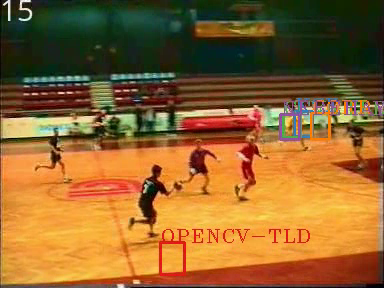
\includegraphics[width=\columnwidth]{handball1-example.png}
		\caption{15. slika posnetka \textit{handball1}.}
		\label{fig:handball1}
	\end{subfigure}
	~
	\begin{subfigure}[t]{0.45\columnwidth}
		\includegraphics[width=\columnwidth]{/handball2-example.png}
		\caption{111. slika posnetka \textit{handball2}.}
		\label{fig:handball2}
	\end{subfigure}  
	\caption[Primer delovanja sledilnikov za \textit{handball} posnetke]{Primer delovanja sledilnikov za \textit{handball} posnetke. Referenčni igralec, ki mu morajo slediti ima rumeno majico. }
	\label{fig:tracker-visual}
\end{figure}




Čeprav smo z mero določili, da se je najbolje izkazal sledilnik CORR, se je pri hitri vizualni oceni sledenja na izsekih posnetka \cite{squashtv2014squash} izkazalo, da najbolje deluje sledilnik KCF. Primer boljšega delovanja KCF sledilnika je slika \ref{fig:squash-tracker-visual}, kjer sledimo modremu igralcu. Na isti sliki posnetka je KCF algoritem našel modrega igralca, medtem ko ga je CORR algoritem zamenjal z drugim igralcem. 



\begin{figure}[!htbp]
	\centering
	\includegraphics[width=0.6\columnwidth]{preliminary-tracker-squash.png}
	\caption{}
	\caption[Primer delovanja sledilnikov za squash posnetek]{Primer delovanja sledilnikov za squash posnetek. Gre za 41. sliko posnetka \cite{squashtv2014squash}, pri čemer smo uporabili KCF in CORR algoritem. Sledilnika sta morala slediti igralcu z modro majico.}
	\label{fig:squash-tracker-visual}
\end{figure}


Boljše delovanje KCF je razumljivo, saj prvi testi temeljijo na posnetkih rokometa, drugi pa na squashu, kjer gre za bistveno drugačno igro. Če pogledamo tabelo \ref{tab:region-overlap} ima KCF drugo najboljše povprečje, prav tako pa so si rezultati posameznih posnetkov zelo podobni. 


















\subsection{Observabilnost}
Rezultate observabilnosti lahko vidimo v tabeli \ref{tab:observabilnost}. Validacijske metrike so povprečne vrednosti \textit{sv} in \textit{bv} modelov, brez križnega testiranja.  Personov korelacijski koeficient smo povprečili s Fisherjevo $z$ transformacijo. Tako energijska poraba kot srčni utrip, imata visoko pozitivno korelacijo, kar pomeni, da sta oba parametra observabilna. \textit{hr} modeli se po CORR rezultatih bolje ujemajo z referenco, vendar moramo pri tem upoštevati tudi nSV razmerje, ki je tu večje. Če primerjamo metrike napak, \textit{eem} modeli prekašajo \textit{hr} modele. S tem lahko potrdimo, da srčni utrip ni dober fiziološki parameter za določevanje fizične aktivnosti. Najboljši rezultati predikcije energijske porabe in srčnega utripa so prikazani na sliki \ref{fig:stage1-observability}.

\begin{table}[!htbp]
\centering
\begin{tabular}{l S[table-format=1.2, round-mode=places, round-precision=2] S[table-format=1.2, round-mode=places, round-precision=2] S[table-format=1.2, round-mode=places, round-precision=2] S[table-format=1.2, round-mode=places, round-precision=2]}
	\toprule
	\textbf{Model} & \thead{CORR} & \thead{RAE} & \thead{RRSE} & \thead{nSV} \\
		\midrule
		\tdata{observabilnost}
		\bottomrule
		\end{tabular}
		\caption{Validacijske metrike testa observabilnosti. Gre za povprečne vrednosti \textit{sv} in \textit{bv} modelov. Personov korelacijski koeficient (CORR) smo povprečili s Fisherjevo $z$ transformacijo.}
	\label{tab:observabilnost}
	\end{table}
	
\begin{figure}[!htbp]
\centering
\includegraphics[width=0.5\columnwidth]{best-results-normal--sideview-sideview-normal-sl}
\caption{Najboljši reultati predikcije energijske porabe in srčnega utripa. Slika prikazuje izhode eem-sv(sv) in hr-sv(sv) modelov ter izmerjene vrednosti energijske porabe in srčnega utripa.}
	\label{fig:stage1-observability}
	\end{figure}


\subsection{Ročni izrez}
Tabela \ref{tab:rocni-izrez} prikazuje rezultate ročnega izreza. Prikazani so tudi rezultati observabilnosti za primerjavo. Validacijske metrike so povprečne vrednosti \textit{sv} in \textit{bv} modelov, brez križnega testiranja.  Personov korelacijski koeficient smo povprečili s Fisherjevo $z$ transformacijo. Rezultati modelov z ročnim izrezovanjem so za malenkost slabši. Še vseeno smo jih uporabili v nadaljnih testih, ker se z njimi teoretično znebimo šuma ozadja.

\begin{table}[!htbp]
	\centering
	\begin{tabular}{l S[table-format=1.2, round-mode=places, round-precision=2] S[table-format=1.2, round-mode=places, round-precision=2] S[table-format=1.2, round-mode=places, round-precision=2] S[table-format=1.2, round-mode=places, round-precision=2]}
		\toprule
		\textbf{Model} & \thead{CORR} & \thead{RAE} & \thead{RRSE} & \thead{nSV} \\
		\midrule
		\tdata{rocni-izrez}
		\bottomrule
	\end{tabular}
	\caption{Validacijske metrike testov ročnega izreza. Gre za povprečne vrednosti \textit{sv} in \textit{bv} modelov. Personov korelacijski koeficient (CORR) smo povprečili s Fisherjevo $z$ transformacijo.}
	\label{tab:rocni-izrez}
\end{table}
		
\subsection{Modaliteta}
Rezultati posameznega pogleda kamere so vidni v tabeli \ref{tab:zorni-kot}. Slike smo pred procesiranjem ročno izrezali tako, da smo določili območje tarče, kjer smo zaobjeli celoten subjekt glede na vse sekvence video posnetka. S tem smo simulirali idealni sledilnik. Rezultate tako lažje primerjamo s terenskimi testi.
		
	\begin{table}[!htbp]
	\centering
	\begin{tabular}{l S[table-format=1.2, round-mode=places, round-precision=2] S[table-format=1.2, round-mode=places, round-precision=2] S[table-format=1.2, round-mode=places, round-precision=2] S[table-format=1.2, round-mode=places, round-precision=2]}
\toprule
\textbf{Model} & \thead{CORR} & \thead{RAE} & \thead{RRSE} & \thead{nSV} \\
\midrule
\tdata{zorni-kot}
	\bottomrule
	\end{tabular}
		\caption{Rezultati modalitete zornega kota kamere.}
		\label{tab:zorni-kot}
		\end{table}
		
Če primerjamo \textit{bv(bv)} in \textit{sv(sv)} modele dobimo pri slednjih boljše rezultate. Slabši rezultati hrbtne kamere bi lahko nakazovali na to, da je ta pogled manj informativen. Pri opazovanju križnih testov (testi s podatki različnega pogleda) lahko vidimo, da dobimo pri vseh slabe rezultate. CORR je zelo nizek ali negativen, metrike napak pa so zelo visoke. Glavna razlika mešanih modelov je opazna šele s primerjavo modelov s križnim testiranjem. Rezultati mešanih modelov so veliko boljši in nakazujejo na to, da lahko dobimo boljše rezultate, če uporabimo podatke iz različnih zornih kotov.

Rezultati različne modalitete glede na tip slike so prikazani v tabeli \ref{tab:zorni-kot}. Tudi tu smo posamezne slike sekvenc posnetkov ročno izrezali. V tabeli je prikazana primerjava \textit{ir} in \textit{bv} modelov. \textit{sv} modelov tu ni, saj smo snemali le hrbtne IR posnetke. Rezultati IR posnetkov so boljši, kar se še posebno opazi pri modelih predikcije srčnega utripa.

\begin{table}[!htbp]
\centering
\begin{tabular}{l S[table-format=1.2, round-mode=places, round-precision=2] S[table-format=1.2, round-mode=places, round-precision=2] S[table-format=1.2, round-mode=places, round-precision=2] S[table-format=1.2, round-mode=places, round-precision=2]}
\toprule
\textbf{Model} & \thead{CORR} & \thead{RAE} & \thead{RRSE} & \thead{nSV} \\
\midrule
\tdata{crop-ir}
	\bottomrule
	\end{tabular}
		\caption{Validacijske metrike za različne modalitete glede na tip slike (BGR ali IR).}
		\label{tab:crop-ir}
		\end{table}
	


















\subsection{Modeliranje dodatne zakasnitve}
Modeli z dodatno zakasnitvijo so v tabeli \ref{tab:lag} označeni z \textit{lag}. Opazimo lahko, da so vsi rezultati s zakasnitvijo, ne glede na modaliteto, boljši. Z \textit{lag} modeli smo potrdili predpostavko o zakasnitvi \SI{55}{\s} za energijsko porabo in \SI{15}{\s} za srčni utrip. Ker smo z njimi rešili probleme sinhronizacije, smo jih uporabili v nadaljnih raziskavah. 

\begin{table}[!htbp]
	\centering
	\begin{tabular}{l S[table-format=1.2, round-mode=places, round-precision=2] S[table-format=1.2, round-mode=places, round-precision=2] S[table-format=1.2, round-mode=places, round-precision=2] S[table-format=1.2, round-mode=places, round-precision=2]}
		\toprule
		\textbf{Model} & \thead{CORR} & \thead{RAE} & \thead{RRSE} & \thead{nSV} \\
		\midrule
		\tdata{crop-lag}
		\bottomrule
	\end{tabular}
	\caption{Primerjava rezultatov med modeli z dodatno zakasnitvijo in brez.}
	\label{tab:lag}
\end{table}



\begin{figure}[!htbp]
	\centering
	\includegraphics[width=0.5\columnwidth]{best-results-crop-normal-infrared-infrared-lag-sl}
	\caption{Najboljši reultati predikcije energijske porabe in srčnega utripa z upoštevanjem dodatne zakasnitve. Slika prikazuje izhode eem-ir-lag(ir) in hr-ir-lag(ir) modelov ter izmerjene vrednosti energijske porabe in srčnega utripa.}
	\label{fig:crop-lag-rezultat}
\end{figure}

















\subsection{Obremenitveni testi}
Rezultati obremenitvenih testov so prikazani v tabelah \ref{tab:crop-proj} in \ref{tab:crop-scale}. Opazimo lahko, da dobimo pri uporabi IR posnetkov slabše rezultate glede na tabelo \ref{tab:lag}. IR posnetki tako niso primerni za terenske raziskave, saj tam pri snemanju nimamo nikoli idelanih pogojev.

\begin{table}[!htbp]
	\centering
	\begin{tabular}{l S[table-format=1.2, round-mode=places, round-precision=2] S[table-format=1.2, round-mode=places, round-precision=2] S[table-format=1.2, round-mode=places, round-precision=2] S[table-format=1.2, round-mode=places, round-precision=2]}
		\toprule
		\textbf{Model} & \thead{CORR} & \thead{RAE} & \thead{RRSE} & \thead{nSV} \\
		\midrule
		\tdata{crop-proj}
		\bottomrule
	\end{tabular}
	\caption{Validacijske metrike rezultatov s projektivno transformacijo slik posnetkov.}
	\label{tab:crop-proj}
\end{table}

\begin{table}[!htbp]
	\centering
	\begin{tabular}{l S[table-format=1.2, round-mode=places, round-precision=2] S[table-format=1.2, round-mode=places, round-precision=2] S[table-format=1.2, round-mode=places, round-precision=2] S[table-format=1.2, round-mode=places, round-precision=2]}
		\toprule
		\textbf{Model} & \thead{CORR} & \thead{RAE} & \thead{RRSE} & \thead{nSV} \\
		\midrule
		\tdata{crop-sc}
		\bottomrule
	\end{tabular}
	\caption{Rezultati obremenitvenega testa skaliranja.}
	\label{tab:crop-scale}
\end{table}










\subsection{Tekalna steza s sledenjem}
Pri testiranju vpeljve sledilnika smo dobili rezultate v tabeli \ref{tab:shake}. Z vpeljavo sledilnika smo dobili celo nekoliko boljše rezultate od tistih z ročnim izrezovanjem (tabela \ref{tab:lag}). To si lahko razlagamo s tem, da je z uporabo sledilnika določitev območja tarče bolj optimalno, saj je območje določeno za vsako sliko posebej. Zaradi tega so modeli bolj robustni na šum ozadja.

%Results of models with enabled tracker are represented in Table \ref{tab:tracker-models-validation}. If we compare them with results of initial models in Table \ref{tab:initial-models-validation}, the mean absolute difference of RRSE between them is \SI{28}{\%}. We can assume that this is due to the fact that tracker does not track selected object perfectly. In some cases it cannot find object, or detects wrong object. It can also track only part of the object. This anomalies can affect calculation of physiological parameters.



\begin{table}[!htbp]
	\centering
	\begin{tabular}{l S[table-format=1.2, round-mode=places, round-precision=2] S[table-format=1.2, round-mode=places, round-precision=2] S[table-format=1.2, round-mode=places, round-precision=2] S[table-format=1.2, round-mode=places, round-precision=2]}
		\toprule
		\textbf{Model} & \thead{CORR} & \thead{RAE} & \thead{RRSE} & \thead{nSV} \\
		\midrule
		\tdata{shake}
		\bottomrule
	\end{tabular}
	\caption{Tracker normal and tracker shake}
	\label{tab:shake}
\end{table}


Srednja absolutna razlika RRSE metrike med modeli s sledenjem in simulacijo vibracij je okoli \SI{30}{\%}. Rezultati s simulacijo vibracij so slabši, vendar še vedno sprejemljivi, saj sledilnik bolje stabilizira posnetek.











\subsection{Terenski eksperimenti squash igre}
Terenski rezultati squash igre z različnimi deskriptorji so predstavljeni v tabeli \ref{tab:squash}.  Rezultatov ne moremo pravilno evaluirati, ker imamo preobremenjene modele. Zaključimo lahko, da postopek 1. faze ne moremo uporabljati za terenske eksperimente. Odziv preobremenjenih modelov lahko vidimo na sliki \ref{fig:squash-rezultat}.

\begin{table}[!htbp]
	\centering
	\begin{tabular}{l S[table-format=1.2, round-mode=places, round-precision=2] S[table-format=1.2, round-mode=places, round-precision=2] S[table-format=1.2, round-mode=places, round-precision=2] S[table-format=1.2, round-mode=places, round-precision=2]}
		\toprule
		\textbf{Model} & \thead{CORR} & \thead{RAE} & \thead{RRSE} & \thead{nSV} \\
		\midrule
		\tdata{squash-mag}
		\bottomrule
	\end{tabular}
	\caption{Validacijske metrike terenskega testiranja. Tu uporabljamo HOOF in HOOF-HAFA deskriptorje. Modeli so neveljavni.}
	\label{tab:squash}
\end{table}

\begin{figure}[!htbp]
	\centering
	\includegraphics[width=0.5\columnwidth]{best-results-preliminary-squash2-normal-backview-backview-lag-sl}
	\caption{Odziv modela hr-bv-lag-hoofhafa(bv) za squash igro eksperimentov 1. faze.}
	\label{fig:squash-rezultat}
\end{figure}






















\subsection{Eksperiment detekcije dihanja}
Za detekcijo dihanja, ki smo jo formulirali kot problem razrščanja v razrede, smo uporabili standardne metrike za evaluacijo dvorazrednega problema. ``Diha'' smo označili kot pozitivno vrednost, ``ne diha'' pa negativno. Dobili smo sledeče rezultate: Razmerje napačno potrjenih FPR = \SI{13}{\%}, razmerje pravilno potrjenih TPR = \SI{87}{\%}, razmerje napačno zavrnjenih FNR = \SI{26}{\%}, razmerje pravilno zavrnjenih TNR = \SI{74}{\%}. Rezultati so prav tako prikazani s kontigenčno matriko na sliki \ref{fig:breathtest-confusion} in ROC krivuljno \ref{fig:breathtest-roc}.

\begin{figure}[!htbp]
	\centering
	\includegraphics[width=0.5\linewidth]{breathtest-confusion-sl}
	\caption{Kontigenčna matrika med ciljnim in izhodnim razredom za detekcijo dihanja. Razred $1$ pomeni ``diha''. Razred $0$ pomeni ``ne diha''.}
	\label{fig:breathtest-confusion}
\end{figure}

\begin{figure}[!htbp]
	\centering
	\includegraphics[width=0.5\linewidth]{breathtest-roc-sl}
	\caption{ROC krivulja za detekcijo dihanja.}
	\label{fig:breathtest-roc}
\end{figure}




























\section{Eksperimenti 2. faze}
\subsection{Preliminarni eksperimenti}
\subsubsection{Združevanje slik iz dveh Kinect kamer}\label{sec:rezultati-zdruzevanje}
Združevanje s značilkami se ni obneslo, zato smo to metodo opustili. Primer neuspelega poskusa je prikazan na sliki \ref{fig:zdruzevanje-znacilke}.

\begin{figure}[!htb]
	\centering
	\begin{subfigure}[t]{0.45\columnwidth}
		\includegraphics[width=\columnwidth]{./Slike/matched-features.png}
		\caption{Ujemajoče SURF značilke}
		\label{fig:zdruzevanje-surf}
	\end{subfigure}
	~
	\begin{subfigure}[t]{0.45\columnwidth}
		\includegraphics[width=\columnwidth]{./Slike/features-calibration-result.png}
		\caption{Rezultat združevanja z značilkami}
		\label{fig:zdruzevanje-result}
	\end{subfigure}
	\caption{Primer neuspelega poskusa združevanja slik iz dveh Kinect kamer s SURF značilkami.}
	\label{fig:zdruzevanje-znacilke}
\end{figure}

 Rezultat združevanja s kontrolnimi točkami je bil boljši od združevanja z značilkami, vendar še vedno slab, zato smo tudi to metodo opustili. Primer neuspelega poskusa je prikazan na sliki \ref{fig:zdruzevanje-cp}.
 
 \begin{figure}[!htb]
 	\centering
 	\begin{subfigure}[t]{0.45\columnwidth}
 		\includegraphics[width=\columnwidth]{matched-points.png}
 		\caption{Ujemajoče kontrolne točke}
 		\label{fig:zdruzevanje-ujemajoce-cp}
 	\end{subfigure}
 	~
 	\begin{subfigure}[t]{0.45\columnwidth}
 		\includegraphics[width=\columnwidth]{points-calibration-result.png}
 		\caption{Rezultat združevanja s kontrolnimi točkami}
 		\label{fig:zdruzevanje-result-cp}
 	\end{subfigure}
 	\caption{Primer neuspelega poskusa združevanja slik iz dveh Kinect kamer s kontolnimi točkami.}
 	\label{fig:zdruzevanje-cp}
 \end{figure}











\subsubsection{Optimizacija Gaussovega filtra}
Rezultati povrprečnih vrednosti uporabljenih metrik so vidni v tabeli \ref{tab:gauss}. Za pravilno razlago rezultatov, moramo upoštevati tudi grafe metrik posameznih eksperimentov, ki so prikazani na slikah \ref{fig:sigma1-5}, \ref{fig:sigma-rmse5-21} in \ref{fig:sigma21-51}. 



\begin{table}[!htb]
	\centering
	\begin{tabular}{S[table-format=2.0, round-mode=places, round-precision=2] S[table-format=1.2, round-mode=places, round-precision=2] S[table-format=2.2, round-mode=places, round-precision=2]}
		\toprule
		\thead{$\mathbf{\sigma}$} & \thead{RMSE} & \thead{SNR [dB]}  \\
		\midrule
		1 & 4.7764 & 24.1892\\
		3 & 6.3162 & 25.5183\\
		5 & 6.5385 & 25.8459\\
		11 & 6.6457 & 26.1244\\
		21 & 6.6794 & 26.2933\\
		31 & 6.6951 & 26.3922\\
		51 & 6.7155 & 26.5345\\
		\bottomrule
	\end{tabular}
	\caption[Povprečne vrednosti RMSE in SNR metrik pri optimizaciji parametra $\sigma$ Gaussovega filtra]{Povprečne vrednosti RMSE in SNR metrik pri optimizaciji parametra $\sigma$ Gaussovega filtra. Najmanjši standardni odklon ima najmanjšo napako, vendar je tudi filtriranje majhno. Pri $\sigma=3$ in $\sigma=5$ so še opazne razlike pri filriranju. Za višje vrednosti ni več opazne razlike, vendar pa se napaka povečuje. $\sigma=5$ je tako optimalna vrednosti parametra.}
	\label{tab:gauss}
\end{table}

Najmanjšo napako dobimo, če uporabimo $\sigma=1$, vendar pa imamo pri tem najmanjše filtriranje, zato so rezultati še vedno lahko zelo šumni. Z višanjem parametra filtra, se napaka po metriki RMSE povečuje, vendar ima večji vpliv razmerje SNR, saj je predstavljeno v logaritemski skali. 

\begin{figure}[!htb]
	\centering
	\begin{subfigure}[t]{0.45\columnwidth}
		\includegraphics[width=\columnwidth]{sigma-rmse1-5-sl}
		\caption{Graf RMSE  učnih vzorcev }
		\label{fig:sigma-rmse1-5}
	\end{subfigure}
	~
	\begin{subfigure}[t]{0.45\columnwidth}
		\includegraphics[width=\columnwidth]{sigma-snr1-5-sl}
		\caption{Graf SNR  učnih vzorcev}
		\label{fig:sigma-snr1-5}
	\end{subfigure}
	\caption{Grafa RMSE in SNR učnih vzorcev za \mbox{$\sigma \in [1,5]$}}
	\label{fig:sigma1-5}
\end{figure}

Čeprav pri uporabi $\sigma=51$ dobimo največje filtriranje šuma, lahko na slikah grafov opazimo, da se obe metriki bistveno ne razlikujeta za vrednosti parametra na intervalu $[5,51]$. Kljub dobremu filtriranju želimo zagotoviti čim manjšo napako med referenčnim signalom in predikcijo, zato je logična izbira čim manjši standardni odklon. Ker so na sliki \ref{fig:sigma1-5} med $\sigma=3$ in $\sigma=5$ še opazne razlike, lahko zaključimo, da je $\sigma=5$ optimalna izbira parametra za naš problem. 


\begin{figure}[!htb]
	\centering
	\begin{subfigure}[t]{0.45\columnwidth}
		\includegraphics[width=\columnwidth]{sigma-rmse5-21-sl}
		\caption{Graf RMSE  učnih vzorcev}
		\label{fig:sigma-rmse5-21}
	\end{subfigure}
	~
	\begin{subfigure}[t]{0.45\columnwidth}
		\includegraphics[width=\columnwidth]{sigma-snr5-21-sl}
		\caption{Graf SNR  učnih vzorcev}
		\label{fig:sigma-snr5-21}
	\end{subfigure}
	\caption{Grafa RMSE in SNR učnih vzorcev za \mbox{$\sigma \in [5,21]$}}
	\label{fig:sigma5-21}
\end{figure}



\begin{figure}[!htb]
	\centering
	\begin{subfigure}[t]{0.45\columnwidth}
		\includegraphics[width=\columnwidth]{sigma-rmse21-51-sl}
		\caption{Graf RMSE učnih vzorcev}
		\label{fig:sigma-rmse21-51}
	\end{subfigure}
	~
	\begin{subfigure}[t]{0.45\columnwidth}
		\includegraphics[width=\columnwidth]{sigma-snr21-51-sl}
		\caption{Graf SNR  učnih vzorcev}
		\label{fig:sigma-snr21-51}
	\end{subfigure}
	\caption{Grafa RMSE in SNR učnih vzorcev za \mbox{$\sigma \in [21,51]$}}
	\label{fig:sigma21-51}
\end{figure}


\subsubsection{Rezultati mrežnega iskanja \texorpdfstring{$\nu$}{nu}-RBF}
Rezultati optimizacije parametra $\numax$ so predstavljeni v tabeli \ref{tab:nu-max}. Pri validaciji ni opaznih sprememb med različnim parametrom $\numax$ zaradi slabih modelov, zato smo preverili verifikacijo. Pri verifikaciji lahko opazimo, da se s povečevanjem parametra povečuje število podpornih vektorjev, vendar nSV nikoli ne doseže željene vrednosti $\numax$. Kljub podoptimalnosti modelov, z višjimi vrednostmi $\numax$ dobimo boljše rezultate. Razlike med $\numax=0.5$ in $\numax=0.8$ so minimalne zato lahko zaključimo, da potrebujemo za dobro delovanje vsaj $\numax=0.5$. 

\begin{table}[!htbp]
	\centering
	\begin{tabular}{l S[table-format=1.2, round-mode=places, round-precision=2] S[table-format=1.2, round-mode=places, round-precision=2] S[table-format=1.2, round-mode=places, round-precision=2] S[table-format=1.2, round-mode=places, round-precision=2]}
		\toprule
		\textbf{Model} & \thead{CORR} & \thead{RAE} & \thead{RRSE} & \thead{nSV} \\
		\midrule
		\tdata{nu-max}
		\bottomrule
	\end{tabular}
	\caption{Verifikacijske metrike pri optimizaciji parametra $\numax$ postopka mrežnega iskanja \nurbf.}
	\label{tab:nu-max}
\end{table}


Tabela \ref{tab:rbf-nu} predstavlja primerjavo med postopkom z uporabo \nurbf in brez. Metrike so povprečne vrednosti \textit{sv} in \textit{bv} modalitet, pri čemer nismo upoštevali ročnega izrezovanja slik. Pearsonov korelacijski koeficient (CORR) smo povprečili s Fisherjevo $z$ transformacijo. Rezultati nakazujejo, da lahko z uporabo \nurbf dobimo izboljšane rezultate.

\begin{table}[!htbp]
	\centering
	\begin{tabular}{l S[table-format=1.2, round-mode=places, round-precision=2] S[table-format=1.2, round-mode=places, round-precision=2] S[table-format=1.2, round-mode=places, round-precision=2] S[table-format=1.2, round-mode=places, round-precision=2]}
		\toprule
		\textbf{Model} & \thead{CORR} & \thead{RAE} & \thead{RRSE} & \thead{nSV} \\
		\midrule
		\tdata{rbf-nu}
		\bottomrule
	\end{tabular}
	\caption{Validacijske metrike za primerjavlo med postopkom z \nurbf in brez. Gre za povprečne vrednosti \textit{sv} in \textit{bv} modelov. Personov korelacijski koeficient (CORR) smo povprečili s Fisherjevo $z$ transformacijo.}
	\label{tab:rbf-nu}
\end{table}




\begin{comment}
\subsubsection{Jedro GHI}
\begin{table}[!htbp]
	\centering
	\begin{tabular}{l S[table-format=1.2, round-mode=places, round-precision=2] S[table-format=1.2, round-mode=places, round-precision=2] S[table-format=1.2, round-mode=places, round-precision=2] S[table-format=1.2, round-mode=places, round-precision=2]}
		\toprule
		\textbf{Model} & \thead{CORR} & \thead{RAE} & \thead{RRSE} & \thead{nSV} \\
		\midrule
		\bottomrule
	\end{tabular}
	\caption{Ghi vmax800}
	\label{tab:ghi}
\end{table}

\begin{figure}[!htbp]
	\centering
	\caption{Ghi best - eem-sv-lag(sv)}
	\label{fig:ghi}
\end{figure}
\end{comment}


\subsubsection{Normalizacija HAFA deskriptorja}
V tabeli \ref{tab:norm-hafa} dobimo slabe rezultate tako za NORMAL model kot tudi za DIAG model, kjer upoštevamo amplitudni faktor $f_A$. Kljub temu so rezultati z upoštevanjem diagonale boljši, kar nakazuje tudi slika \ref{fig:corr-diag}.

\begin{table}[!htbp]
	\centering
	\begin{tabular}{l S[table-format=1.2, round-mode=places, round-precision=2] S[table-format=1.2, round-mode=places, round-precision=2] S[table-format=1.2, round-mode=places, round-precision=2] S[table-format=1.2, round-mode=places, round-precision=2]}
		\toprule
		\textbf{Model} & \thead{CORR} & \thead{RAE} & \thead{RRSE} & \thead{nSV} \\
		\midrule
		\tdata{diag}
		\bottomrule
	\end{tabular}
	\caption{Evaluacijske metrike pri primerjavi modelov NORMAL in DIAG, kjer upoštevamo amplitudni faktor $f_A$. }
	\label{tab:norm-hafa}
\end{table}

\begin{figure}[!htb]
	\centering
	\begin{subfigure}[t]{0.45\columnwidth}
		\includegraphics[width=\columnwidth]{diag-normal-corr-sl}
		\caption{Korelacija za NORMAL model.}
		\label{fig:corr-diag-normal}
	\end{subfigure}
	~
	\begin{subfigure}[t]{0.45\columnwidth}
		\includegraphics[width=\columnwidth]{diag-diag-corr-sl}
		\caption{Korelacija za DIAG model.}
		\label{fig:corr-diag-diag}
	\end{subfigure}
	\caption[]{Grafa korelacij za NORMAL in DIAG model. Kljub slabim rezultatom obeh modelov, je DIAG model občutno boljši.}
	\label{fig:corr-diag}
\end{figure}


\subsection{Laboratorijski eksperiementi}
\subsubsection{Odvisnost na akumulacijo utrujenosti}
V tabeli \ref{tab:stage2-lab-1-mean} je predstavljeno povprečje validacij merjencev za protokol 1. Personov korelacijski koeficient (CORR) smo povprečili s Fisherjevo $z$ transformacijo. Vsi modeli imajo visoko korelacijo z referenco. Napake so majhne. Opazimo, da dobimo boljše rezultate z uporabo prostorskega toka \textit{it}.

\begin{table}[!htbp]
	\centering
	\begin{tabular}{l S[table-format=1.2, round-mode=places, round-precision=2] S[table-format=1.2, round-mode=places, round-precision=2] S[table-format=1.2, round-mode=places, round-precision=2] S[table-format=1.2, round-mode=places, round-precision=2]}
		\toprule
		\textbf{Model} & \thead{CORR} & \thead{RAE} & \thead{RRSE} & \thead{nSV} \\
		\midrule
		\tdata{stage2-lab-1-mean}
		\bottomrule
	\end{tabular}
	\caption{Povprečje validacij merjencev za protokol 1 druge faze laboratorijskih eksperimentov. Personov korelacijski koeficient (CORR) smo povprečili s Fisherjevo $z$ transformacijo.}
	\label{tab:stage2-lab-1-mean}
\end{table}

V tabeli \ref{tab:stage2-lab-2-mean}  predstavljamo povprečje rezultatov za protokol 2. Personov korelacijski koeficient (CORR) smo povprečili s Fisherjevo $z$ transformacijo. Vsi modeli imajo pričakovano nizko korelacijo in veliko napak.

\begin{table}[!htbp]
	\centering
	\begin{tabular}{l S[table-format=1.2, round-mode=places, round-precision=2] S[table-format=1.2, round-mode=places, round-precision=2] S[table-format=1.2, round-mode=places, round-precision=2] S[table-format=1.2, round-mode=places, round-precision=2]}
		\toprule
		\textbf{Model} & \thead{CORR} & \thead{RAE} & \thead{RRSE} & \thead{nSV} \\
		\midrule
		\tdata{stage2-lab-2-mean}
		\bottomrule
	\end{tabular}
	\caption{Povprečje validacij merjencev za protokol 2 druge faze laboratorijskih eksperimentov. Personov korelacijski koeficient (CORR) smo povprečili s Fisherjevo $z$ transformacijo.}
	\label{tab:stage2-lab-2-mean}
\end{table}

Glede na rezultate v tabelah \ref{tab:stage2-lab-1-mean} in  \ref{tab:stage2-lab-2-mean} se utrujenost akumulira skozi čas, kar moramo upoštevati pri gradnji modelov.


\subsubsection{Generalizacija modela}
S protokolom 3 smo želeli preveriti, če lahko uporabimo generaliziran model za predikcijo energijske porabe na različnih merjencih. Rezultati so vidni v tabeli \ref{tab:stage2-lab-3}. Zanimivo dobimo najboljše rezultate za optični tok in ne za prostorskega, kot smo predlagali. Korelacije modelov z optičnim tokom \textit{of} se bližajo vrednosti $1$, vendar pa so metrike napak slabše. Nakazujejo na to, da modeli le niso tako zelo dobri. Vsekakor imamo podobne rezultate tako za SUBJ8 kot za SUBJ9, kar naznanja dobro generalizacijo modela.

\begin{table}[!htbp]
	\centering
	\begin{tabular}{l S[table-format=1.2, round-mode=places, round-precision=2] S[table-format=1.2, round-mode=places, round-precision=2] S[table-format=1.2, round-mode=places, round-precision=2] S[table-format=1.2, round-mode=places, round-precision=2]}
		\toprule
		\textbf{Model} & \thead{CORR} & \thead{RAE} & \thead{RRSE} & \thead{nSV} \\
		\midrule
		%\tdata{stage2-lab-3}
		\bottomrule
	\end{tabular}
	\caption{Validacijske metrike za protokol 3 druge faze laboratorijskih eksperimentov.}
	\label{tab:stage2-lab-3}
\end{table}

Najboljši rezultati za optični in prostoski tok, so predstavljeni na sliki \ref{fig:lab-3}. Odzivi modelov vsebujejo veliko šuma, zato bi lahko uporabili širše Gaussovo jedro za filtriranje rezultatov. Najslabšo predikcijo dobimo za največjo fizično aktivnost.

\begin{figure}[!htbp]
	\centering
	\begin{subfigure}[t]{0.45\columnwidth}
		%\includegraphics[width=\columnwidth]{best-results-stage3-lab-of-3-subj6-sideview-sideview-normal-sl}
		\caption{Rezultati eem-sv-of-subj9(sv) z optičnim tokom}
		\label{fig:lab-of-3}
	\end{subfigure}
	~
	\begin{subfigure}[t]{0.45\columnwidth}
		%\includegraphics[width=\columnwidth]{best-results-stage3-lab-sf-3-subj6-sideview-sideview-normal-sl}
		\caption{Rezultati eem-sv-sf-subj9(sv) s prostorskim tokom}
		\label{fig:lab-sf-3}
	\end{subfigure}
	\caption[Odziv SUBJ9 modelov protokola 3 druge faze laboratorijskih eksperimentov]{Odziv najboljših modelov protokola 3 druge faze laboratorijskih eksperimentov. Rdeča krivulja predstavlja merjen parameter, zelena predikcijo. Na sliki \subref{fig:lab-of-3}) je najboljši rezultat pri uporabi optičnega toka. Na sliki \subref{fig:lab-sf-3}) je najboljši rezultat pri uporabi prostorskega toka.}
	\label{fig:lab-3}
\end{figure}

\subsection{Terenski eksperimenti}
\subsubsection{Odvisnost na akumulacijo utrujenosti}
V tabeli \ref{tab:stage2-field-1-mean} je predstavljeno povprečje validacij merjencev za protokol 1. Personov korelacijski koeficient (CORR) smo povprečili s Fisherjevo $z$ transformacijo. Najboljše rezultate dobimo za prostorski tok \textit{sf}. Korelacija je dokaj visoka, ampak metrike napak nakazujejo na slabši model.

\begin{table}[!htbp]
	\centering
	\begin{tabular}{l S[table-format=1.2, round-mode=places, round-precision=2] S[table-format=1.2, round-mode=places, round-precision=2] S[table-format=1.2, round-mode=places, round-precision=2] S[table-format=1.2, round-mode=places, round-precision=2]}
		\toprule
		\textbf{Model} & \thead{CORR} & \thead{RAE} & \thead{RRSE} & \thead{nSV} \\
		\midrule
		\tdata{stage2-field-1-mean}
		\bottomrule
	\end{tabular}
	\caption{Povprečje validacij merjencev za protokol 1 druge faze terenskih eksperimentov. Personov korelacijski koeficient (CORR) smo povprečili s Fisherjevo $z$ transformacijo.}
	\label{tab:stage2-field-1-mean}
\end{table}

V tabeli \ref{tab:stage2-field-2-mean} predstavljamo povprečje rezultatov za protokol 2. Personov korelacijski koeficient (CORR) smo povprečili s Fisherjevo $z$ transformacijo. Vsi modeli imajo pričakovano nizko korelacijo in veliko napak.

\begin{table}[!htbp]
	\centering
	\begin{tabular}{l S[table-format=1.2, round-mode=places, round-precision=2] S[table-format=1.2, round-mode=places, round-precision=2] S[table-format=1.2, round-mode=places, round-precision=2] S[table-format=1.2, round-mode=places, round-precision=2]}
		\toprule
		\textbf{Model} & \thead{CORR} & \thead{RAE} & \thead{RRSE} & \thead{nSV} \\
		\midrule
		\tdata{stage2-field-2-mean}
		\bottomrule
	\end{tabular}
	\caption{Povprečje validacij merjencev za protokol 2 druge faze terenskih eksperimentov. Personov korelacijski koeficient (CORR) smo povprečili s Fisherjevo $z$ transformacijo.}
	\label{tab:stage2-field-2-mean}
\end{table}

\subsubsection{Generalizacija modela}
S protokolom 3 smo želeli preveriti, če lahko uporabimo generaliziran model za predikcijo energijske porabe na različnih merjencih. Rezultati so vidni v tabeli \ref{tab:stage2-field-3}. Tukaj dobimo najboljše rezultate pri uporabi prostorskega toka, kot smo to predlagali tudi sami. Tudi rezultati optičnega toka niso slabi. Najboljši rezultati za optični in prostoski tok, so predstavljeni na sliki \ref{fig:lab-3}.

\begin{table}[!htbp]
	\centering
	\begin{tabular}{l S[table-format=1.2, round-mode=places, round-precision=2] S[table-format=1.2, round-mode=places, round-precision=2] S[table-format=1.2, round-mode=places, round-precision=2] S[table-format=1.2, round-mode=places, round-precision=2]}
		\toprule
		\textbf{Model} & \thead{CORR} & \thead{RAE} & \thead{RRSE} & \thead{nSV} \\
		\midrule
		\tdata{stage2-field-3}
		\bottomrule
	\end{tabular}
	\caption{Validacijske metrike za protokol 3 druge faze terenskih eksperimentov.}
	\label{tab:stage2-field-3}
\end{table}

\begin{figure}[!htbp]
	\centering
	\begin{subfigure}[t]{0.45\columnwidth}
		\includegraphics[width=\columnwidth]{best-results-stage3-final-field-of-3-subj6-backview-backview-normal-val-sl}
		\caption{Rezultati eem-bv-of-subj9(bf) z optičnim tokom}
		\label{fig:field-of-3}
	\end{subfigure}
	~
	\begin{subfigure}[t]{0.45\columnwidth}
		\includegraphics[width=\columnwidth]{best-results-stage3-final-field-sf-3-subj6-backview-backview-normal-val-sl}
		\caption{Rezultati flow eem-bv-sf-subj9(bv) s prostorskim tokom}
		\label{fig:field-sf-3}
	\end{subfigure}
	\caption[Odziv SUBJ9 modelov protokola 3 druge faze laboratorijskih eksperimentov]{Odziv najboljših modelov protokola 3 druge faze laboratorijskih eksperimentov. Rdeča krivulja predstavlja merjen parameter, zelena predikcijo. Na sliki \subref{fig:field-of-3}) je najboljši rezultat pri uporabi optičnega toka. Na sliki \subref{fig:field-sf-3}) je najboljši rezultat pri uporabi prostorskega toka.}
	\label{fig:field-3}
\end{figure}











\chapter{Diskusija}\label{sec:diskusija}
V tem delu smo raziskali novo brezkontaktno metodo za estimacijo fizioloških parametrov iz gibanja. Za določitev parametrov smo uporabljali algoritme optičnega in prostorskega toka, ki smo jih kombinirali s kombinacijami HOOF in HAFA deskriptorjev. S tem smo zagotovili robustnost algoritmov. Za predikcijo energijske porabe in srčnega utripa smo uporabili SVM regresijo, pri tem pa smo razvili \nurbf postopek mrežnega iskanja za optimizacijo. Za izločevanje šuma iz ozadja in gibanja neopazovanih objektov smo uporabljali sledilnike ter Kalmanov in Gaussov filter.

Rezultati kažejo na ta to, da so izbrani fiziološki parametri \emph{observabilni}. Predlagano metodo lahko uporabimo z različnimi sistemi za vizualno zaznavanje z različnih zornih kotov. Boljše rezultate lahko dobimo z uporabo posnetkov iz več zornih kotov. Elementarni modeli iz prve faze eksperimentov niso primerni za terensko uporabo. Pri učenju modelov moramo biti pozorni na akumulacijo utrujenosti. Za laboratorijske preiskave je bolje, če uporabimo metode z optičnim tokom. Na terenu dobimo najboljše rezultate z uporabo prostorskega toka.

Za dela~\cite{peker2004framework,silva2015assessing,osgnach2010energy} rezultatov ne moremo primerjati, ker v njih uporabljajo subjektivne mere. Prav tako ne vsebujejo nobene primerjave z uveljavljeno referenco indirektne kalorimetrije.

Če primerjamo delo~\cite{botton2011energy} z našimi končnimi generaliziranimi modeli s prostorskim tokom faze 2, dobimo boljše rezultate. V delu~\cite{botton2011energy} je korelacijski koeficient $\corr=\num{0.93}$. Naš znaša $\corr=\num{0.995}$ za laboratorijske in $\corr=\num{0.999}$ za terenske teste. 

V~\cite{nathan2015estimating} je konkordančni korelacijski koeficient $CCC=\num{0.879}$, napaka pa znaša $\rmse=\SI{2.004}{\kcal}$. Za naše najboljše laboratorijske modele s prostorskim tokom faze 2 dobimo $CCC=\num{0.989}$ in $\rmse=\SI{9.870}{\kcal}$. Za najboljše terenske modele s prostorskim tokom faze 2 so metrike  $CCC=\num{0.983}$ in $\rmse=\SI{4.234}{\kcal}$. V obeh primerih dobimo boljše korelacije, vendar pa so napake dosti večje. Napako bi lahko izboljšali z večanjem števila podpornih vektorjev in dodatnim glajenjem izhodnih signalov.

Avtorji so v~\cite{gjoreski2015context} uporabili podoben pristop našemu, le da so namesto brezkontaktnih uporabili kontaktne senzorje. Z njihovim MCE pristopom so dobili $\rmse=\SI{1.192}{MET}$ za aktivnosti teka. V delu navajajo tudi metriko za BodyMedia senzor. Gre za trenutno najboljši komercialno dosegljiv kontaktni senzor za estimacijo energijske porabe. Njegova metrika je znašala $\rmse=\SI{2.458}{MET}$ za aktivnosti teka. V našem primeru dobimo $\rmse=\SI{8.111}{MET}$ za laboratorijske modele s prostorskim tokom faze 2 in $\rmse=\SI{4.098}{MET}$ za terenske modele s prostorskim tokom faze 2. Rezultati so po izbranih metrikah dokaj slabi. 

Kljub obetavnim rezultatom, metoda vsebuje še kar nekaj problemov, ki jih moramo rešiti v prihodnje. Nimamo modela z upoštevanjem časovne dinamike. Globinske slike Kinect senzorja vsebujejo veliko šuma, ki bi ga mogli pred procesiranjem čim bolj odpraviti. Združevanje slik iz dveh Kinect kamer ni idealno. Potrebovali bi bolj avtomatično metodo. V postopku bi lahko dodali nove najboljše sledilnike. S tem bi pridobili še večjo natančnost sistema. Modele faze 2 bi morali dodatno optimizirati, da bi dobili manjši šum na izhodu.

%**************** LITERATURA ************************
\bibliographystyle{ieeetrslo}
\bibliography{./bib/experiments,./bib/fatigue,./bib/features,./bib/filters,./bib/hr-motion-sensor,./bib/image-stitching,./bib/main,./bib/metabolism,./bib/metrics,./bib/optical-flow,./bib/physical-activity,./bib/related-work,./bib/scene-flow,./bib/sleep-apnoea,./bib/svm,./bib/tracking} 

%**************** PRILOGE ************************
%\appendix

\end{document}
